%!TEX TS-program = pdflatexmk
\documentclass[11pt]{book}
\usepackage{graphicx}
\DeclareGraphicsRule{.tiff}{png}{.png}{`convert #1 `dirname #1`/`basename #1 .tiff`.png}

\usepackage{amsmath,amssymb}
\usepackage{times}
\usepackage{epstopdf}
\usepackage[ligature,reserved]{semantic}
\usepackage[center,tight]{subfigure}
\usepackage{proof}

\usepackage{longtable}

\usepackage{color}

\definecolor{red}{rgb}{1,0,0}
\definecolor{magenta}{cmyk}{0,1,0,0}
\definecolor{halfgrey}{gray}{0.5}

\textwidth = 6.5 in
\textheight = 9 in
\oddsidemargin = 0.0 in
\evensidemargin = 0.0 in
\topmargin = 0.0 in
%\headheight = 0.0 in
%\headsep = 0.0 in
\parskip = 3pt
\parindent = 0.0in

%no indent on footnotes
\makeatletter
\renewcommand{\@makefntext}[1]{\setlength{\parindent}{0pt}%
\begin{list}{}{\setlength{\labelwidth}{1em}%
  \setlength{\leftmargin}{\labelwidth}%
  \setlength{\labelsep}{3pt}\setlength{\itemsep}{0pt}%
  \setlength{\parsep}{0pt}\setlength{\topsep}{0pt}%
  \footnotesize}\item[\hfill\@makefnmark]#1%
\end{list}}
\makeatother

%\newtheorem{theorem}{Theorem}
%\newtheorem{corollary}[theorem]{Corollary}
%\newtheorem{definition}{Definition}

\title{{\huge Roll your own Jape logic}\\
             Encoding logics for the Jape proof calculator}
\author{Richard Bornat (richard@bornat.me.uk)%\\
        %Bernard Sufrin (sufrin@comlab.ox.ac.uk)
       }

\mathlig{->}{\rightarrow}
\mathlig{=>}{\Rightarrow}
\mathlig{|->}{\mapsto}
\mathlig{|-}{\vdash}
\mathlig{|=}{\vDash}
\mathlig{|*}{\exists}
\mathlig{|}{\lor}
\mathlig{!}{\neg}
\mathlig{@*}{\forall}
\mathlig{@}{\land}
\mathlig{<->}{\leftrightarrow}
\mathlig{<|}{\triangleleft}

\mathlig{++}{\mathbin{+\!\,+}}
\mathlig{--}{\mathbin{-\!\,-}}

\reservestyle{\word}{\operatorname}

\reservestyle{\var}{\mathit}

\reservestyle{\textword}{\text}
\textword{true,false}

% BAN symbols
\def\believes{\mathrel\mid\joinrel\equiv}
\def\oncesaid{\mathrel\mid\joinrel\sim}
\def\sees{\mathrel\triangleleft}
\def\hasjurisdictionover{\mathrel\mid\joinrel\Rightarrow}
\def\fresh{\#}

\usepackage{ucs}
\usepackage[utf8x]{inputenc}
\usepackage[T1]{fontenc}
\newcommand{\textGamma}{\ensuremath{\Gamma}}
\newcommand{\textDelta}{\ensuremath{\Delta}}
\newcommand{\textalpha}{\ensuremath{\alpha}}
\newcommand{\textbeta}{\ensuremath{\beta}}
\newcommand{\textlambda}{\ensuremath{\lambda}}
\DeclareUnicodeCharacter {8614}{\ensuremath{|->}}
\DeclareUnicodeCharacter {8870}{\ensuremath{|-}}
\DeclareUnicodeCharacter {8871}{\ensuremath{|=}}
\DeclareUnicodeCharacter {9665}{\ensuremath{\triangleleft}}

\newcommand{\eqnref}[1]{(\ref{eqn:#1})}
\newcommand{\figref}[1]{figure \ref{fig:#1}}
\newcommand{\Figref}[1]{Figure \ref{fig:#1}}
\newcommand{\tabref}[1]{table \ref{tab:#1}}
\newcommand{\Tabref}[1]{Table \ref{tab:#1}}
\newcommand{\secref}[1]{section \ref{sec:#1}}
\newcommand{\Secref}[1]{Section \ref{sec:#1}}
\newcommand{\chapref}[1]{chapter \ref{chap:#1}}
\newcommand{\Chapref}[1]{Chapter \ref{chap:#1}}
\newcommand{\appxref}[1]{appendix \ref{appx:#1}}
\newcommand{\Appxref}[1]{Appendix \ref{appx:#1}}
                                                                                                    
\newcommand{\reason}[1]{\scalebox{0.85}{#1}}

\newcommand {\cols}[1][*{50}{l}]{\begin{array}{#1}}
\newcommand {\sloc}{\end{array}}

\newcommand{\BRA}{\left(\cols}
\newcommand{\KET}{\sloc\right)}
\newcommand{\BRACE}{\left\{\cols}
\newcommand{\ECARB}{\sloc\right\}}

\newcommand{\hstrut}[1]{\rule{#1}{0pt}}
\newcommand{\vstrut}[1]{\rule{0pt}{#1}}

\newcommand{\tab}{\hstrut{10pt}}

\newenvironment{japeish}{\begin{quote}\tt\small}{\end{quote}}
\newcommand{\textj}[1]{{\tt\small{#1}}}

\newenvironment{ruletab}[1]{\renewcommand{\arraystretch}{3.0}\begin{center}\begin{tabular}{#1}}%
{\end{tabular}\end{center}}

%\includeonly{GUIlang}
\usepackage[pagebackref]{hyperref}

\begin{document}
\maketitle

\chapter*{Preface}

Jape is a lightweight, uncommitted, transparent proof calculator. It's designed to present an excellent graphical interface and a very short and shallow `learning curve' to all its users, whether novices learning how to make formal proofs or experts --- logicians, teachers, sofware engineers, practitioners of any kind --- describing inference systems. This manual is directed at people who have experimented with one or more of the inference systems distributed with Jape and now want to develop something of their own, or those who just want to understand what it is that Bernard Sufrin and I have done in our own encodings.


The chapters of this manual describe by example how to encode several interesting logics in Jape. They are intended to be read in sequence, as the earlier chapters give most description of the early stages of the encoding, and later chapters concentrate on more esoteric features.


A manual which described a task only by example would be inadequate, and I therefore include a complete description of the various internal `languages' of Jape:

\begin{itemize}
\item the \emph{term} or \emph{formula} or \emph{sequent} language, in which problems are stated, and which appears on-screen when a proof is displayed --- described in \appxref{paraformlang};
\item the \emph{tactic} language, which includes the statement of the inference rules of a logic, and which allows the user to control the course of a proof --- described in \appxref{tacticlang};
\item the \emph{paragraph} language, which is the notation used to describe a logic and its associated tactics and stuff to Jape --- described in \appxref{paraformlang};
\item the \emph{dialogue} language, which is the notation in which the graphical interface sends commands to the main proof engine, and in which you can type as text in a graphical interface window --- described in \appxref{GUIlang}.
\end{itemize}

This manual doesn't discuss how to use Jape --- that's covered in other manuals. The graphical illustrations are taken from the MacOS X implementation (version 7\_d4 or later).

\section*{Maintenance only}

Jape was once several experiments in one. One was an experiment in user interfaces: could we make a really nice proof calculator? Another was an experiment in abstraction: could we make it customisable? Another was educational: could we teach logic with it? And no doubt there were others which I've now forgotten.

The Jape idea isn't dead, but I think it's safe to say that Bernard and I have found other things to do with our time, and the project is stalled. It's open source, so it could conceivably get started under other hands, but I made it so damn complicated that I don't expect that will happen. Jape is now maintenance-only, though if anybody has a really good simple idea to improve it I might get itchy again.

Because of its architecture and detail internal design, some things which you might think really easy to do are in fact rather hard. So: no apologies for the following list of deficiencies, none of which are likely to be fixed.

\begin{itemize}
\item Jape doesn't check the proof store when you redefine a rule or theorem, and re-run all the proofs that depend on it (though it does guard against circularities in proofs).
\item Jape can't handle sequents in which one side is an optional single formula.
\item Jape has no treatment of definitional equality (syntactic equivalence), so you have to handle it with rules and inference steps.
\item Jape has a long-standing problem in that it can't encode `families of rules'. Bernard employed considerable ingenuity to allow you to encode finite collections of slightly different rules, but that's the nearest you'll get.
\item Jape's parser generator is horribly complicated, but extremely limited.
\item I never quite reached modal logic, and now I never will.
\item Separation logic is right out of the question.
\end{itemize}

I'll add to this list as further deficiencies are pointed out. Mail to bugs@jape.org.uk, please.

\section*{Inadequacies}

Jape started out as a Good Idea which was patched and modified to do more than it perhaps should do. I wrote this manual long after much of the work was done. You may find places in the text where I simply say that I can't remember something or other, or you may find that there are features of Jape which are used in example code but not explained in this manual. Please notify me via bugs@jape.org.uk whenever you notice anything like that.
\tableofcontents
\chapter{Basic Principles}
\label{chap:basics}

Jape works by applying inference rules to sequents in proof trees. Its fundamental mechanism is unification, laced with a pragmatic treatment of explicit substitution forms. We decided on unification rather than one-way pattern-matching because it allows us to use Jape as a Prolog-style calculator, solving question-problems such as
\begin{quote}
$\lambda x.\lambda y.(x\;y): \_T$
\end{quote}
which would be completely intractable, or pointless, in a one-way-matching engine.

Tactics in Jape organise the application of other tactics. The simplest tactic is an inference rule.

On top of its basic proof mechanism Jape provides you with the opportunity to control the graphical user interface by programming its response to the basic gestures of pointing and clicking, and by defining what is included in the menus and panels shown to the user.

\section{Flexible syntax}

Jape has a built-in collection of syntactic forms which you can customise and to which you can add the particular details which are appropriate to your particular logic. It recognises numbers, strings, identifiers, unknowns, bracketed formulae, tuples, substitutions, juxtapositions, and formulae made by using user-defined prefix, postfix and infix operators, with user-defined priorities and associativity. In addition you can invent various new kinds of brackets and punctuation.

Identifiers --- names like $A$, $x$ or $F$ in conjectures, theorems and rules --- rarely stand for themselves. For the most part they stand for some arbitrary formula, variable or predicate which can appear in an instance of the conjecture, theorem or rule in which they are used. When you define the syntax of identifiers in your logic you say which are schematic identifiers and which are constants. At the same time you can define the syntactic category of the identifiers you use.

The flexible syntax mechanism is illustrated in every chapter, and detailed in \appxref{paraformlang}.

%\section{Backward proof}

%Jape always, always, always works backwards --- from conclusion towards antecedents --- even when its display mechanism tries to produce the illusion that it is working forwards. It always works with trees --- Gentzen trees --- of sequents, even when its display mechanism is trying to produce the illusion that it is working with Fitch boxes, or something else. Currently you (or the user) can choose between tree display and box-and-line display for proofs, and there is a treatment of transitional reasoning within box-and-line. We have the beginnings of a more attractive treatment of equational chaining proofs (see, for example, \chapref{funcprog}) and we dream of a kind of Fitchery for linear logic, and more.}. If you haven't seen a Gentzen tree, you can learn how Jape handles them if you use one of the distributed logics that uses tree display mode, or you can switch to tree display mode in one of the distributed logics that allows it --- for example the single-conclusion sequent calculus encoding.

\section{Inference rule matching}

Consider an example rule of the single-conclusion sequent calculus:
\begin{quote}
$\infer[\reason{∨⊦}]
       {\Gamma,A|B |- C}
       {\Gamma,A |- C & \Gamma,B |- C}$
\end{quote}

Its rendition in Japeish (see the file SCS\_rules.j) is a straightforward linearisation.
\begin{quote}
\tt RULE "∨⊦" FROM Γ, A ⊦ C AND Γ, B ⊦ C INFER Γ, A∨B ⊦ C
\end{quote}

Jape's interpretation of the rule is as a description of a node in a proof tree by pattern: the consequent at that node has a collection of formulae on its left-hand side, one of which matches $A|B$ for some pair of formulae $A$ and $B$ and the rest of which are taken as $\Gamma$, and a single right-hand side formula which matches $C$. The node has two antecedents, each of which contains a sequent with the same right-hand side formula $C$. The left-hand antecedent will have a sequent whose left-hand side is $\Gamma$ together with the formula $A$; the right-hand antecedent's left-hand side is $\Gamma$ together with $B$.

Jape makes proofs by unifying (i.e. matching) consequents of rules to tips of the tree, and replacing the tip with the corresponding node. With the exception of \textsc{resolve} and \textsc{cutin} steps, described later, that's \emph{all} it does. Bernard and I, like many before us, fixed on that simple mechanism because we thought we had a chance of getting it right. It means that Jape only works backwards --- from consequent to antecedents --- even when it seems not to be.

The single rule above contains lots of different kinds of symbol. There are the schematic identifiers $\Gamma$, $A$, $B$ and $C$: there is the connective $|$; there are the punctuation marks ⊦ and comma; there's the (quoted) rule name ∨⊦; and there are the reserved words of Japeish \textsc{rule}, \textsc{from}, \textsc{and} and \textsc{infer}. Not all the logical identifiers are schematic: $|$ is in a sense an identifier, but it plays a fixed syntactic r\^{o}le in the logic and in the rule. Apart from the connectives, other identifiers might be non-schematic: there could be constant identifiers $\<true>$ and $\<false>$, for example. As logic describer you have control over the matter, which you exercise by organising identifiers into syntactic categories. This not only allows you to distinguish between schematic and other identifiers, but it also allows you to distinguish, for example, between names like $A$ which might be taken to stand for some arbitrary formula, and names like $x$ which you might wish to stand only for variables.

\textit{Parameters of rules}
\label{sec:basics:parameters}

In simple cases the fact that Jape uses unification rather than one-way pattern matching doesn't have a visible effect on the course of a proof. But if a rule doesn't have the subformula property --- if there are names in its antecedents that don't appear in its consequent, as for example in
\begin{quote}
$\infer[\reason{$!-I$}]
       {\Gamma  |- !A}
       {\Gamma,A |- B@!B}$
\end{quote}
--- then \emph{unknowns} may appear in the proof in place of the schematic identifier $B$.\footnote{This is a \textit{strength} of Jape, not a weakness: we don't require the user to decide prematurely on the identity of those unknowns. As a logic designer, however, you can decide not to let your users see very many unknowns: see \chapref{I2L}, for example}

In these and other circumstances it can be useful to allow the user to provide an argument formula which modifies the instantiation step. You do that by writing the rule definition with a parameter. The rule above is written in Japeish as
\begin{quote}
\tt RULE "¬-I"(B) IS FROM Γ,A ⊦ B∧¬B INFER Γ ⊦ ¬A
\end{quote}
Given a problem sequent $E,F->!E |- !F$, Jape first instantiates the rule by replacing all the schematics with corresponding unknowns; then it unifies \_Γ with $E,F->!E$ and $\_A$ with $F$; thus it generates the antecedent $E,F->!E,F |- \_B@!\_B$ . If it is given the argument formula $E$ to unify with $\_B$, it will generate the antecedent $E,F->!E,F |- E@!E$ . In many cases an argument supplied to the application of a rule can prevent a startling proliferation of unknowns in a proof.

The parameter of a rule may in some circumstances be decorated with the word \textsc{object}. That indicates that in the absence of a user-supplied argument, the instantiation step is to generate a freshly-minted identifier in its place rather than a fresh unknown. Frequently this is because the rule expresses a generalisation step in the logic and it is natural for Jape to mint a fresh name. For example, the rule
\begin{quote}
$\infer[\reason{\textsc{(fresh }$c$, $c$ \textsc{notin} $|*x.A$) ∃-E}]
       {\Gamma |- C}
       {\Gamma  |-|*x.A & \Gamma,A[x\backslash c] |- C}$
\end{quote}
is written as
\begin{quote}
\tt RULE "∃-E"(OBJECT c) WHERE FRESH c AND c NOTIN ∃x.A IS \\
\tab FROM Γ ⊦ ∃x.A AND Γ,A[x\textbackslash c] ⊦ C INFER Γ⊦C
\end{quote}
\textsc{Object} parameters can be used in other circumstances --- in particular, see the discussion of substitution unification below.

\section{Explicit provisos}

Lots of rules have side conditions: the ∃-E rule above, for example, has two. There are traditional ways of dealing with these in proof machinery. Jape takes the simplistic route and includes explicit, visible \emph{provisos} in the proof. Jape's provisos at present are \textsc{notin} and \textsc{unifieswith}, plus three macro-relatives of \textsc{notin}: \textsc{fresh, hypfresh} and \textsc{concfresh}.

Provisos are either satisfied or violated, and they constrain the application of rules. If an attempted application would violate a proviso, whether one contained in the rule itself or one left over from an earlier stage of the proof, then the attempt fails. If it is impossible to determine the status of a proviso, because it contains unknowns and/or substitution forms, then it is stored, displayed as part of the proof, and carried forward in the expectation that its status will become clearer.

The proviso $x$ \textsc{notin} $E$ is satisfied if $x$ doesn't appear free in $E$, and violated if it does --- or rather, it is satisfied if $x$ \emph{cannot} appear free in $E$, no matter what future unifications may happen and no matter how the schematic identifiers of the conjecture being proved are instantiated. The proviso $x$ \textsc{notin} $y$, for example, is not trivially satisfied if $x$ and $y$ are schematic parameters of a  conjecture being proved, even though visibly $y$ is not the same variable as $x$.

\textsc{notin} provisos are either included in the statement of a rule or generated from \textsc{fresh, hypfresh} or \textsc{concfresh} provisos: \textsc{fresh} $x$ generates a proviso $x$ \textsc{notin} $E$ for every left- and right-hand side formula $E$ of the sequent matching the rule; \textsc{hypfresh} $x$ generates \textsc{notin} provisos only for the left-hand side formulae and \textsc{concfresh} for the right-hand side formulae.

\var{E1,E2}
The proviso $\<E1>$ \textsc{unifieswith} $\<E2>$ is internally generated. It allows Jape to defer difficult unifications where it can't find a most-general unifier. This can arise because of difficulties in unifying substitution forms, or when using multiplicative (context-splitting) rules. It plays a r\^{o}le in Jape's drag-and-drop mechanism for resolving context splits: see below.

\section{Conjectures and theorems}

We allow the user to state a conjecture using the \textsc{theorem} directive.\footnote{Bernard and I had rows over this notation. I wanted to emphasise that it's a conjecture till it's proved; he wanted to emphasise that it is theorems, after all, that you are trying to prove. I still think I was righter than he was.} A proved conjecture becomes a theorem and can then be applied as a derived rule. If the state variable \texttt{applyconjectures} is set to $\<true>$ then unproved conjectures can be applied as well.

The \textsc{theorem} directive gives the name of a conjecture and its sequent, and it may also include provisos which will be enforced both during the proof of the conjecture and whenever the theorem is applied. It is possible to define a theorem without giving a name, in which case the sequent itself is used as the name. The \textsc{theorems} directive allows you to state a collection of conjectures, and will give each its own sequent as a name. For example, the SCS.jt file defines a conjecture called \textit{contradiction}
\begin{quote}
\tt THEOREM contradiction IS A, ¬A ⊦ B
\end{quote}
and the sequent\_problems.j file includes a large collection of conjectures named by their sequent, some of which are as follows:
\begin{quote}\tt
THEOREMS PropositionalProblems ARE\\
\tab P→(Q→R) ⊦ (P→Q)→(P→R)\\
AND\tab P→(Q→R), Q ⊦ P→R\\
\tab ....\\
AND\tab WHERE x NOTIN P INFER P ∧ ¬P, ∀x.P→Q, ∀x. ¬P→Q ⊦ ∀x.Q \\
AND\tab R ∧ ¬R, ∀x.R→S, ∀x. ¬R→S ⊦ ∀x.S\\
....\\
AND\tab ∃y.P ⊦ ∀y.P\\
END
\end{quote}
The conjectures in this illustration are called ``P→(Q→R) ⊦ (P→Q)→(P→R)'', ``P→(Q→R), Q ⊦ P→R'', ``P∧¬P, ∀x.P→Q, ∀x.¬P→Q ⊦ ∀x.Q'' (the provisos aren't part of the name), ``R∧ R, ∀x.R→S, ∀x.¬R→S ⊦ ∀x.S'' and ``∃y.P ⊦ ∀y.P''.

\subsection{Proving a conjecture --- substitutions and provisos}

A proof of a conjecture begins with a tree which consists of the base sequent of the conjecture, together with any provisos which were included in the statement of the conjecture\footnote{Jape sometimes adds invisible provisos which it deduces from the binding structure of the formulae in the conjecture: see below, and also \appxref{GUIlang}.}. The proof is then developed by application of rules and tactics.

One important feature of the proof is Jape's treatment of the identifiers and unknowns that appear in the base sequent of the conjecture, and its treatment of other identifiers that may be introduced during the proof process. Jape's theorems are theorem schemata, not particular theorem formulae; they may therefore be instantiated in the same way as a rule, replacing identifiers in the theorem sequent by unknowns or arbitrary formulae. Identifiers in the conjecture's sequent can't, therefore, be treated as standing for themselves during the proof.

In practice this means that substitution forms involving those identifiers may not be simplifiable: if, for example, identifiers $A$ and $x$ appears in the conjectured sequent then $A[x\backslash E]$ can't be replaced by $A$ unless it is certain that there will never be an instance of the theorem in which the formula which instantiates $A$ has a free occurrence of the variable which instantiates $x$. But if $x$ is a name introduced during the proof --- for example, by application of a rule which has an \textsc{object} parameter --- and if there aren't any unknowns remaining which would allow $x$ to be smuggled into the sequent finally proved, then we reason that whatever argument formula instantiates $A$, we could choose $x$ within the proof to be distinct from all the names in $A$, and therefore $A[x\backslash E]$ can be replaced by $A$. In other circumstances the assurance that $x$ can't occur free in $A$ can come from a \textsc{notin} proviso, or from meta-theoretical reasoning about the relationships of names in the conjectured sequent.

Provisos that are introduced during proof of a conjecture, by application of rules or other theorems or conjectures, and which aren't evidently satisfied or violated are retained as part of the theorem and checked whenever the theorem is applied.

The effect of our care with substitutions and provisos is that the proof tree which establishes the validity of a conjecture stands for all the proof trees of all the instances of that conjecture, and Jape is justified in using such a conjecture as a derived rule.

\subsection{Applying a theorem: the r\^{o}le of structural rules}
\label{sec:basics:application}

A theorem is, in principle, a rule with no antecedents. So Jape can instantiate it as a rule and match it to a problem sequent just as a rule is matched. There are, however, a couple of interesting points.

The first is that in many cases a theorem won't have enough left-hand or right-hand side formulae to completely match a problem sequent. The theorem ``P→(Q→R) ⊦ (P→Q)→(P→R)'', for example, matches only sequents with exactly one formula on the left of the turnstile and one on the right. Often a logic will include so-called `weakening' rules which enable you to delete a formula from the left- or the right-hand side or both. If you include such rules and declare their r\^{o}le to Jape, it will allow you to apply a theorem even though it does not completely match a problem sequent.

The second difficulty is that sometimes a theorem matches on the right-hand side, but not on the left. In such a case it is often convenient to prove it `by resolution': that is, to generate an antecedent for each of the left-hand side formulae and to set about proving them. That step is justified if the logic contains a `cut' rule which enables you to move formulae from left- to right-hand side and a `weaken' rule as well. Jape will make a resolution step for you if you declare the appropriate structural rules in your logic, declare their r\^{o}les, and also set the \texttt{tryresolution} variable (see \appxref{GUIlang}) or use one of the \textsc{applyorresolve} or \textsc{resolve} tacticals (see \appxref{tacticlang}).

\section{Substitution forms and unification}

Jape uses explicit substitution forms --- $A[x\backslash c]$, $B[x,y,z\backslash E,F,G]$ --- where some logics use predicate notation --- $P(c)$, $Q(E,F,G)$ . Substitutions are more powerful than predicates because they are more general; for the same reason they are trickier to handle. Jape's internal mechanisms are based on substitution forms, but there is also a mechanism which allows you to write rules and theorems in terms of predicate formulae --- see `interpreting predicates' below.

Explicit substitution forms are semantically scandalous, a notorious trap for novices, and an expert will ask ``what does a substitution form in a rule or theorem \emph{mean}?''. It's difficult to give a simple answer. It is never necessary to include special rules to treat substitution forms --- their treatment is a fundamental mechanism of Jape, and Jape tries to eliminate substitution forms from the proof whereever and whenever they appear. Therefore we can say that Jape treats a substitution form as equivalent to the result of carrying out the subsitution. But in some situations it can be persuaded to treat a substitution form as a structural pattern and will unify one unreduced substitution form with another, even though such unifications don't give the most general answer.

A substitution form is introduced into a proof, and if possible immediately eliminated, whenever the antecedent of a rule contains one. Consider, for example, the problem sequent $x>y |-|*z.z>y$ . If we apply the rule
\begin{quote}
$\infer[|-\exists] {\Gamma|-|*x.A,\Delta} {\Gamma|-A[x\backslash E],\Delta}$
\end{quote}
then we generate a single antecedent $x>y |- (z>y)[z\backslash \_E]$, which immediately simplifies to $x>y |- \_E>y$ provided that we know that $z$ and $y$ are necessarily distinct,\footnote{They might not be if, for example, they both appear in the base sequent of the conjecture being proved. They may be if, for example, one or the other has been generated during the development of the proof, or if there is an explicit proviso which makes it clear that they are distinct.} or to $x>y |- \_E>y[z\backslash \_E]$ otherwise.

Even more interesting is what happens when a rule contains an explicit substitution form such as $A[x\backslash E]$ in its \emph{consequent}. When the rule is applied Jape must unify that substitution form --- or rather, its instantiated form which in general will be $\_A[\_x\backslash \_E]$ --- with some formula $B$ in the problem sequent. That sort of unification is notoriously difficult, and Jape uses a number of ad-hoc strategies to help.
\begin{enumerate}
\item It simplifies substitution forms whenever possible, in order to avoid the problem.
\item It defers the unification of an irreducible substitution form for as long as possible, so that the results of other unifications can be used to simplify it.
\item If the user provides an argument formula \textit{F} in place of parameter $E$, the instantiated form will be $\_A[\_x\backslash F]$ ; when Jape can no longer avoid unifying that form with $B$ it will search for all instances of \textit{F} inside $B$ and try to construct a substitution form $B' [\_x\backslash F]$ which simplifies to $B$ in presence of the proviso $\_x$ \textsc{notin }$B$; if successful it will unify $\_A$ with $B'$ in a context that records the proviso. The process is far more effective if the parameter $x$ is decorated with the word \textsc{object}, so that the instantiated form becomes $\_A[z\backslash F]$ where $z$ is a fresh variable; the formula $B' [z\backslash F]$ is easier to construct and to simplify, and the proviso $z$ \textsc{notin} $B$ is easier to check\footnote{In fact, because $z$ is a fresh variable, the proviso is usually obviously satisfied. But a proviso is necesssary to constrain the future course of the proof if there are unknowns in $B$. In those and in some other circumstances Jape may also produce \textsc{unifieswith} provisos to cater with the process of abstraction in the nasty bits of $B$.}.
\item If the user text-selects instances of a sub-formula \textit{F} of $B$, then the logic encoding can employ the \textsc{withsubstsel} tactical --- see \chapref{funcprog} and \appxref{tacticlang} --- to calculate $B'$ by replacing just those instances of \textit{F} by a fresh unknown $\_y$; $B' [\_y\backslash F]$ necessarily simplifies to $B$ given the proviso $\_y$ \textsc{notin} $B$; then Jape will match the substitutions structurally, unifying $\_A$ with $B'$, $\_x$ with $\_y$ and $\_E$ with \textit{F} in a context which records the proviso. If the parameter $x$ is decorated with the word \textsc{object} then $\_x$ is replaced by $z$ and the proviso becomes $z$ \textsc{notin} $B$, which is once again easier to check.
\item If all else fails, Jape can generate a proviso $\_A[\_x\backslash \_E]$ \textsc{unifieswith} $B$, and await developments.
\end{enumerate}


If Jape has to unify two substitution forms which have identical variable lists then it matches them structurally. For example, it can unify $A[x,y\backslash A1,A2]$ with $B[x,y\backslash B1,B2]$ by unifying $A$ with $B$, \textit{A1} with \textit{B1}, \textit{A2} with \textit{B2}. This happens rarely and because it doesn't generate the most general unifier it might not be the best thing to do, but pragmatically it seems to work rather well almost every time it is used.

If Jape has to unify substitution forms with different variable lists then it extends one or the other: for example, if it has to unify $A[x\backslash A1]$ with $B[x,y\backslash B1,B2]$ it will try to construct $A'$ such that $A[y\backslash B2]$ simplifies to $A$, and then unify $A[x,y\backslash A1,B2]$ with $B[x,y\backslash B1,B2]$ . In certain circumstances it will even do a bit of α-conversion --- but enough! this explanation is sufficiently complicated already.

The message is that Jape's unification of substitution forms is usefully pragmatic. It does not always generate a most-general unifier but it can, in practice, often generate just the unifier that the user is looking for, especially when the encoding uses the \textsc{letsubstsel}/\textsc{withsubstsel} mechanism (see \chapref{funcprog} and \appxref{tacticlang}) to allow the user to describe the unification to Jape. It most often breaks down when it has to deal with substitutions using variables which also appear in the base sequent of the theorem being proved. That breakdown is, I think, inevitable, (and investigations stopped some time ago).

\subsection{Invisible provisos}

Consider the conjectures $\lambda x.\lambda y.x:T1->T2->T1$ and $@*x.|*y.P(x)=P(y)$ . Clearly, in each case, any instance of the conjecture would have to use two distinct variables. Nothing else would give the right binding structure: $\lambda z.\lambda z.z:\operatorname{int} ->\operatorname{real}->\operatorname{int} $ isn't an instance of the first conjecture, nor $@*z.|*z.Q(z)=Q(z)$ of the second\footnote{Strictly speaking, this second \textit{might} be an instance of the the conjecture, if there are no instances of $z$ in $Q$. These are deep waters...}. But Jape's mechanisms of rule and theorem instantiation don't automatically ensure this: instead, there has to be a proviso such as $x$ \textsc{notin} $y$ in each case. Such provisos are fussy, have to do with the internal mechanisms of Jape, and are difficult to explain to Jape's users. Therefore Jape generates them automatically, from an analysis of the binding structure of every rule and conjecture, and then makes them invisible. You can see the invisible provisos in a proof by setting the \texttt{showallprovisos} variable to $\<true>$.

\subsection{Interpreting predicate notation}

Some of our users prefer predicate notation to substitution, and in certain ways it concisely conveys more information. In the formula $@*x.P(x)$ it is implicit that the predicate formula $P$ doesn't contain any instances of $x$; in the corresponding formula $@*x.P[v\backslash x]$ no such inference can be drawn, and the statement of a theorem which contained such a formula would require a proviso $x$ \textsc{notin} $P$ to say as much as the predicate version. Fussy provisos get substitution notation a bad name, so we have implemented a mechanism which interprets predicate notation, translating it into substitution notation and inserting invisible provisos.\footnote{Those invisible provisos constrain the proof. If they were too constraining, the worst that could happen is that you miss some proofs.} When you apply a rule which contains $@*x.P(x)$, for example, Jape translates it into $@*x.P[v\backslash x]$, automatically inserting $x$ \textsc{notin} $P$. When you begin a proof which contains $@*x.P(x)$, Jape doesn't translate it, but it does insert the same proviso, making it invisible.

If you set the variable \texttt{interpretpredicates} to $\<true>$, Jape treats every juxtaposition as if it were a predicate application. If \texttt{interpretpredicates} is $\<false>$ (the default), Jape only interprets those juxtapositions in which the first formula is an \textsc{abstraction} parameter name. See chapters \ref{chap:ItL} and \ref{chap:funcprog} for examples.

In one respect Jape's interpretation of predicate notation is pragmatically helpful rather than careful. Consider, for example, the sequent $|*x.@*y.P(x,y) |- @*y.|*x.P(x,y)$ . Jape translates this to $|*x.@*y.P[u,v\backslash x,y] |- @*y.|*x.P[u,v\backslash x,y]$, and automatically includes provisos $x$ \textsc{notin} $P$ and $y$ \textsc{notin} $P$, as it should. Jape also includes $x$ \textsc{notin} $y$, which isn't essential in order to preserve the binding structure, because it is not required that either $x$ or $y$ must appear free in a predicate $P(x,y)$ . The effect is that certain instances of the theorem are excluded. In practice it seems that our users prefer it this way.

\section{Binding forms: unification, α-conversion and substitution}

Suppose that $@*var.formula$ has been defined to be a binding form: then Jape will proceed as follows:
\begin{itemize}
\item it will unify $@*x.A$ with $@*x.B$ by unifying $A$ with $B$;
\item it will unify $@*x.A$ with $@*\_y.B$ by unifying $x$ with $\_y$ and $A$ with $B$
\item it will unify $@*x.A$ with $@*y.B$ by unifying $@*z.A[x\backslash z]$ with $@*z.B[y\backslash z]$, where $z$ is a fresh variable, together with the provisos $z$ \textsc{notin} $A$ and $z$ \textsc{notin} $B$.
\end{itemize}

Jape respects binding forms when carrying out substitutions. Thus, for example, if $@*var.formula$ has been defined to be a binding form and $x$ and $y$ are guaranteed distinct then $(@*x.A)[x\backslash E]$ always simplifies to $@*x.A$ and, provided that $x$ doesn't appear free in \textit{F}, $(@*x.A)[y\backslash F]$ will simplify to $@*x.(A[y\backslash F])$; in other circumstances it will simplify to by α-conversion to $@*z.(A[x,y\backslash z,F])$ together with the proviso $z$ \textsc{notin} $A$, where $z$ is a fresh variable.

\section{The tactic language}

Although Jape's basic operation is the application of rules to tips of a proof tree, that is by no means the whole story. You will often find it necessary to organise the application of rules by writing programs in the tactic language.

Bernard originally invented the tactic language\footnote{Over my dead body, several times. This is one battle I'm glad I lost.} to enable us to express programmed actions like proof searches. It's become a workhorse for many more tasks than that.

The simplest tactics are inference rules. You can apply tactics sequentially (\textsc{seq}), or try one after another (\textsc{alt, when}), you can call tactics with arguments, you can repeat tactics (\textsc{do}); there is a notion of the `current goal' sequent in the tree which is used when tactics are applied in sequence. It is possible, under very severe constraints, to transform formulae within the goal sequent (\textsc{find, flatten, withsubstsel}).

Most of the language has to do with the interpretation of gestures and selection of an appropriate response.

\Appxref{tacticlang} gives a complete list of all the verbs of the tactic language. The chapters of this manual give examples of their use.

\section{Gestures, menus and panels}
\label{sec:basics:gestures}

The user can make certain `gestures' at the Jape graphical interface. The way in which the gestures are made --- which buttons and keys are pressed and how the mouse is moved --- depends on the operating system. In general a `click' is a left-button mouse click, a `subformula click' is a middle-button click (or a click with the alt/option key held down).
\begin{itemize}
\item A user can \emph{select} a formula in a sequent by clicking it. If a rule is then applied, Jape requires by default that the selected formula is a principal formula in the rule. Thus, for example, if you select the hypothesis $E|F$ in the sequent $G|H, E|F, G->E |- G@E$ and then apply the rule
\begin{quote}
$\infer[\reason{∨⊦}]
       {\Gamma,A|B |- C}
       {\Gamma,A |- C &  \Gamma,B |- C}$
\end{quote}
you ensure that $A|B$ in the rule matches $E|F$ in the sequent, $\Gamma$ matches $G|H,\;G->E$ and, of course, $C$ matches $G@E$. (A tactic can test for formula selection, discover the formula selected, and modify its behaviour accordingly.)
\item A user can double-click (`hit') on a formula, causing the application of a tactic chosen by the logic description.
\item A user can double-click on the `reason' or `justification' of a proof step. If there is hidden detail behind that step then it will be revealed, or if it has been revealed by an earlier double-click, it will be hidden again.
\item A user can drag a formula. If there is a \textsc{unifieswith} proviso, generated as a result of context-splitting in a multiplicative rule, some of the other formulae mentioned in that proviso --- unknown segment variables like \_Γ or \_Δ1 --- will highlight as the formula is dragged across them.
\item A user can \emph{subformula-select} part or all of a formula in a sequent. If a rule is applied, the subformula is provided as the first argument. If a tactic is applied, it can test for subformula selection and modify its behaviour accordingly.
\item A user can select an entry in a menu, and Jape will carry out the corresponding command. Most entries correspond to the command \texttt{apply T} for some tactic \texttt{T}, but a menu can contain any of the commands listed in \appxref{GUIlang}. A good deal of your user-interface design activity will go into deciding what goes in which menus, fixing on labels for each entry and choosing just the right commands.
\item A user can press a button in a panel, with or without first choosing an entry from the list of entries in the same panel. Many panels list conjectures, and their buttons allow users to prove the chosen conjecture, apply it as a theorem and so on. Other panels may be like menus. The designer controls what is in the entries and what is on the buttons, and whether or not a particular button sends just a command, or a command modified by the selected entry.
\item A user can scroll the proof horizontally and/or vertically.
\end{itemize}


And that's it. Jape uses a very impoverished vocabulary of gesture: we have chosen to make it so, in an attempt to make Jape as straightforward to use as any other application in a modern GUI environments.

\section{Proof display: trees, boxes and hiding}

The Gentzen tree is the basic proof structure on which Jape works. Behind the scenes, whatever is on the screen, is a Gentzen tree. Tactics can be used to hide selected antecedents of a proof step and alter the `reason' or `justification' displayed with the step; the hidden detail can be revealed to a user who double-clicks appropriate parts of the proof.

Gentzen trees are notoriously wasteful of display space, and Fitch boxes famously less so. Jape can display a proof in an approximation to Fitch box style. The display is a transcription --- not a translation --- of the tree, and it can be applied to any kind of logic, not simply natural deduction. This is how it's done:
\begin{itemize}
\item the assumptions --- left-hand side formulae --- of the base sequent are written on the first line and the conclusion(s) --- right-hand side formula(e) --- on the last line;
\item if a line is the conclusion of a proof step then the lines representing the trees of its antecedents are written out before it, working left to right through the antecedents;
\item the justification of a line which is the conclusion of a proof step references the assumption line(s) to describe any left-hand side principal formulae, as well as the lines which contain the conclusions of its antecedents;
\item if a line is the conclusion of a tip then a line of dots is written before it;
\item if an antecedent introduces any hypotheses then its lines are written in a box, whose first line is those hypotheses and whose last line is the right-hand side formula(e) of the antecedent.
\end{itemize}


That makes a fairly compact description, in which hypotheses are written only once but conclusions may be written more often, especially when a left-hand side rule is used. It is made still more compact by hiding applications of \textsc{identity} (aka axiom, hypothesis) rules, and it is made to support some forms of forward reasoning (see chapters \ref{chap:ItL} and \ref{chap:I2L}) by hiding, under the right circumstances, applications of a \textsc{cut} rule.

If you select a conclusion formula in a box display, the effect is just as if you had selected the corresponding conclusion formula in the underlying Gentzen tree. If you select a hypothesis formula the effect can't be so simple, because a hypothesis formula is written only once even though it may occur in many sequents: Jape finds the set of sequents that you could be pointing to and disambiguates the choice using any conclusion selection that you might have made.

It doesn't make sense to use box display with a multiple-conclusion calculus for various reasons, and Jape's gesturing mechanisms therefore haven't been adapted to this use.

Our box display isn't a proper Fitch box display because you can't necessarily use the proof which ends on line $j$ when making a proof step on a subsequent line $k$, even though the box structure would allow it. The reason is that line $j$ may be part of the proof of some cousin of $k$, not part of the proof of $k$ --- that is, parts of the proof which are sequentially related in the box display aren't necessarily hierarchically related in the underlying Gentzen tree. There is a tactic-language solution (see \textsc{cutin} in \chapref{I2L}), but without that Jape provide some assistance by making the underlying tree structure more evident when the user selects an assumption or a conclusion: once you make a selection it will `grey out' lines in the box display which are irrelevant because they are not hierarchically related in the underlying tree.

\section{Using Jape interactively}


Jape starts up `empty', with no theory loaded.

You can load a new theory into Jape by using File:Open New Theory. At any time you can add additional bits of Japeish to the brew, by using File:Open. Jape works, like LISP or ML, by maintaining a store of definitions, and it is always possible to add to those definitions. The effects may be strange, especially if you try to add a new theory without getting rid of the old one first!
 
\chapter{Encoding the Sequent Calculus}
\label{chap:sequentcalculus}

Jape is, at bottom, a backwards-reasoning proof editor working on a tree of sequents. It is therefore no surprise that it is exceptionally straightforward to encode the sequent calculus in Jape. We describe in this chapter the encoding of the multiple-conclusion sequent calculus in the file \texttt{examples/sequent\_calculus/MCS.jt} and the files it references. 

The rules we use, and the examples, were borrowed from Roy Dyckhoff's excellent MacLogic (an inspiring precursor of Jape). This encoding draws heavily on the single-conclusion sequent calculus encoding (see \texttt{examples/SCS.jt}), developed jointly by Bernard Sufrin and myself in the early days of Jape, so `we' is Bernard and me. The encoding is quite old, and the segmentation into files is somewhat arbitrary.

\begin{table}
\centering
\caption{The \texttt{axiom} rule}
\label{tab:seqcalculusaxiom}
\vstrut{20pt}
$\infer[\reason{axiom}]
       {\Gamma,A |- A,\Delta }
       {}$ 
\end{table}

\begin{table}
\centering
\caption{Introduction to the right of the turnstile (⊦... rules)}
\label{tab:sequentleftrules}
\vstrut{30pt}
$\infer[\reason{⊦∧}]
       {\Gamma  |- A@B,\Delta }
       {\Gamma  |- A,\Delta & \Gamma  |- B,\Delta }$
\qquad\vstrut{30pt}
$\infer[\reason{⊦→}]
       {\Gamma  |- A->B,\Delta }
       {\Gamma,A |- B,\Delta }$
\qquad\vstrut{30pt}
$\infer[\reason{⊦∨}]
       {\Gamma  |- A|B,\Delta }
       {\Gamma  |- A,B,\Delta }$
\qquad\vstrut{30pt}
$\infer[\reason{⊦¬ }]
       {\Gamma  |- !A,\Delta }
       {\Gamma,A |- \Delta }$ 
\qquad\vstrut{30pt}
$\infer[\reason{⊦≡}]
       {\Gamma |- A\equiv B, \Delta }
       {\Gamma |- A->B, \Delta & \Gamma |- B->A, \Delta }$
\qquad\vstrut{30pt}
$\infer[\reason{(fresh $m$) ⊦∀}]
       {\Gamma  |- @*x.A(x),\Delta }
       {\Gamma  |- A(m),\Delta }$
\qquad\vstrut{30pt}
$\infer[\reason{⊦∃}]
       {\Gamma  |-|*x.A(x),\Delta }
       {\Gamma  |- A(B),\Delta }$
\end{table}


\begin{table}
\centering
\caption{Introduction to the left of the turnstile (...⊦ rules)}
\label{tab:sequentrightrules}
$\infer[\reason{∧⊦}]
       {\Gamma,A@B |- \Delta }
       {\Gamma,A,B |- \Delta }$
\qquad\vstrut{30pt}
$\infer[\reason{→⊦}]
       {\Gamma,A->B |- \Delta }
       {\Gamma  |- A,\Delta & \Gamma,B |- \Delta }$
\qquad\vstrut{30pt}
$\infer[\reason{∨⊦}]
       {\Gamma,A|B |- \Delta }
       {\Gamma,A |- \Delta & \Gamma,B |- \Delta }$
\qquad\vstrut{30pt}
$\infer[\reason{¬⊦}]
       {\Gamma,!A |- \Delta }
       {\Gamma  |- A,\Delta }$ 
\qquad\vstrut{30pt}
$\infer[\reason{≡⊦}]
       {\Gamma,A->B,B->A|-C}
       {\Gamma,A\equiv B |-C}$
\qquad\vstrut{30pt}
$\infer[\reason{∀⊦}]
       {\Gamma,@*x.A(x)  |- \Delta }
       {\Gamma,A(B)  |- \Delta }$
\qquad\vstrut{30pt}
$\infer[\reason{(fresh $m$) ∃⊦}]
       {\Gamma,|*x.A(x)  |- \Delta }
       {\Gamma,A( m)  |- \Delta }$
\end{table}


\begin{table}
\centering
\caption{Structural rules}
\label{tab:sequentstructuralrules}
$\infer[\reason{cut}]
       {\Gamma  |- \Delta }
       {\Gamma  |- B,\Delta & \Gamma,B |- \Delta }$
\qquad\vstrut{30pt}
$\infer[\reason{⊦ weaken}]
       {\Gamma  |- A,\Delta }
       {\Gamma  |- \Delta }$
\qquad\vstrut{30pt}
$\infer[\reason{⊦ contract}]
       {\Gamma  |- A,\Delta }
       {\Gamma  |- A,A,\Delta }$
\qquad\vstrut{30pt}
$\infer[\reason{weaken ⊦}]
       {\Gamma,A |- \Delta }
       {\Gamma  |- \Delta }$
\qquad\vstrut{30pt}
$\infer[\reason{contract ⊦}]
       {\Gamma,A |- \Delta }
       {\Gamma,A,A |- \Delta }$
\end{table}

\begin{table}
\centering
\caption{Modified quantifier rules}
\label{tab:seqcalculusquantifierrules}
$\infer[\reason{(fresh $m$) ⊦∀}]
       {\Gamma  |- @*x.A,\Delta }
       {\Gamma  |- A[x\backslash m],\Delta }$
\qquad\vstrut{30pt}
$\infer[\reason{⊦∃}]
       {\Gamma  |- |*x.A,\Delta }
       {\Gamma  |- A[x\backslash B],\Delta }$
\qquad\vstrut{30pt}
$\infer[\reason{∀⊦}]
       {\Gamma,@*x.A |- \Delta }
       {\Gamma,A[x\backslash B]  |- \Delta }$
\qquad\vstrut{30pt}
$\infer[\reason{(fresh $m$) ∃⊦}]
       {\Gamma,|*x.A |- \Delta }
       {\Gamma,A[x\backslash m]  |- \Delta }$\vstrut{30pt}
\end{table}

\section{The inference rules of the (multiple-conclusion) Sequent Calculus}

We have encoded a standard version of the sequent calculus. By making our left- and right-hand sides \textit{bags} (aka multisets) of formulae we have avoided the need for exchange rules; by allowing the axiom rule to ignore unnecessary hypotheses and conclusions we have avoided the need to use weakening rules in almost every case and/or to describe context-splitting rules. See \chapref{sequentvariations} for an alternative treatment of quantifiers and variables and for Jape's treatment of context-splitting (multiplicative) rules.

The rules, given in tables \ref{tab:seqcalculusaxiom}, \ref{tab:sequentleftrules}, \ref{tab:sequentrightrules} and \ref{tab:sequentstructuralrules}, are additive --- that is, don't split their left- or right-hand side contexts working backwards. Multiplicative (context-splitting) rules are harder to use in a backwards reasoning tool, because either the tool must force the user to decide how to split the context before the rule is applied or else it must provide machinery to allow the decision to be deferred (Jape chooses deferral: see \chapref{sequentvariations}). In this encoding, the fact that the \textit{axiom} rule ignores unnecessary hypothesis and conclusion formulae makes context-splitting on either side unnecessary.

Because Jape interprets predicate notation as shorthand for substitution, the \textit{actual} quantifier rules use substitution. \Tabref{seqcalculusquantifierrules} shows the rules which Jape employs, translating the originals on input. The difference need hardly detain us: there are no additional provisos, and no substitution-matching is required. In this logic at least, it's easy to believe that Jape manipulates predicate notation directly.


\section{Syntax description (\texttt{sequent\_syntax.j})}

We begin with a couple of variable initialisations:\footnote{The syntactic form we use is that of an assignment to a variable. The \texttt{interpretpredicates} variable can only be altered when the store of rules and variables is empty, so in practice it behaves as a parameter.}
\begin{quote}\tt\small
INITIALISE interpretpredicates true \\
INITIALISE displaystyle tree
\end{quote}
This ensures that juxtapositions are interpreted as predicate application, and that we see the proofs as trees.

We use names starting with A, B, C, D, P, Q, R and S in rules and conjectures to stand for any formula; we use names starting with u, v, w, x, y, z. m or n to stand for any variable. Names starting with Γ or Δ stand for bags (multisets) of formulae\footnote{Note that now there are no commas in these lists of identifier prefixes: I have eliminated use of comma as a separator in the paragraph language. See \appxref{paraformlang} for more details}.

\begin{quote}\tt\small
CLASS BAG Γ ∆ \\
CLASS FORMULA A B C D P Q R S \\
CLASS VARIABLE u v w x y z m n
\end{quote}

These directives also cover unknowns: an unknown which starts $\_A$ will unify with any formula, but one which starts $\_z$ will only unify with a variable or a similar unknown.

Quantifier formulae are, like if-then-else in most programming languages, bracketed without a final closing bracket:
\begin{quote}\tt\small
LEFTFIX 20              ∀ .\\
LEFTFIX 20              ∃ .
\end{quote}
The connectives are defined as operators with particular \emph{binding power} and \emph{binding direction}:
\begin{quote}\tt\small
INFIX           100L            ≡\\
INFIX           110R            →\\
INFIX           150L            ∧\\
INFIX           160L            ∨\\
PREFIX          200             ¬
\end{quote}
The relative binding power of juxtaposition and substitutions are defined:
\begin{quote}\tt\small
JUXTFIX         300 \\
SUBSTFIX        400 
\end{quote}
Working from the bottom, this defines substitution forms as the most binding, then juxtaposition. Next comes ¬ defined as a prefix operator, then the binary connectives (all but → are defined to be left-associative, while → is right-associative). Finally two special bracketed forms are defined, with the lowest syntactic priority. These definitions allow us to write:
\var{prim,f1,f2}
\begin{itemize}
\item $!\<prim>$, where $\<prim>$ is an atomic formula, a substitution or a juxtaposition (see \appxref{paraformlang});

\item $\<f1>|\<f2>$, $\<f1>@\<f2>$ or $\<f1>->\<f2>$ with the interpretation that ∨ `operators' have priority over ∧, and both have priority over →;

\item \ensuremath{@*} $\<f1>$. $\<f2>$ and \ensuremath{|*} $\<f1>$ . $\<f2>$.
\end{itemize}

Note that the leftfix patterns don't constrain you to write ∀\textit{variable}.\textit{formula}: that comes later.

Because there is no closing bracket, formulae constructed with \textsc{leftfix} bracketing are liable to have a visually ambiguous interpretation, so Jape demands that \textsc{leftfix}-brackets aren't used like ordinary brackets: that is, you can't write things like $f1@@*x.f2@f3$ : you have to write instead either $f1@(@*x.f2@f3) $ or $f1@(@*x.f2) @f3$ .

The binding structures are given by pattern:
\begin{quote}\tt\small
BIND    x SCOPE P IN ∃x . P\\
BIND    x SCOPE P IN ∀x . P
\end{quote}
Any formula which matches one of these patterns is recognised as a binding formula --- any variable in place of \textit{x}, any formula, including another binding formula, in place of $P$. Near matches aren't allowed, so the constraint to write \textit{quantifier} \textit{variable}. \textit{formula} is enforced.

Note that this defines only single-variable bindings. Jape has no means at present of defining families of binding structures, except by exhaustively listing them --- for example, you might give \textsc{bind} directives which describe the structure of \ensuremath{@*}\textit{x},y.$E$, \ensuremath{@*}\textit{x},\textit{y},$z$.$E$ and so on as we do in later chapters. But then you would find that Jape has no means of defining families of inference rules which work across the different kinds of bindings you can define, and you would have to separately define the rules --- one for \ensuremath{@*}\textit{x}.$E$, another for \ensuremath{@*}\textit{x},y.$E$, another for \ensuremath{@*}\textit{x},\textit{y},$z$.$E$ and so on.

\section{Encoding the inference rules (\texttt{MCS\_rules.j})}

Our sequents have bags of formulae on either side:

\begin{quote}\tt\small
SEQUENT IS BAG ⊦ BAG
\end{quote}

Jape is designed to make the encoding of inference rules as transparent and straightforward as possible. In principle all you have to do is to linearise the normal description of a rule, giving its name, its provisos, its antecedents and its consequent. Writing \{... \} for optional inclusion and \{... \}* for repeated optional inclusion, the syntax of a \textsc{rule} directive is

\begin{tabular}{lll}
\textsc{rule} & \{ \textit{name} \} & --- \textit{rule name}\\
 & \{ (\textit{parameter} \{, \textit{parameter} \}*) \} & --- \textit{parameters}\\
 & \{ \textsc{where} \textit{proviso} \{\textsc{and} \textit{proviso}\}* \} & --- \textit{provisos}\\
 & \{ \textsc{is} \}\\
 & \{ \textsc{from} \textit{sequent} \{\textsc{and} \textit{sequent}\}* \} & --- \textit{antecedents}\\
 & \textsc{infer} \textit{sequent} & --- \textit{consequent}
\end{tabular}

Nearly everything is optional, but you have to put in enough reserved words to make it clear where each section begins and ends. If you leave the name out, the name is taken to be the consequent itself. Where the name of a rule isn't an identifier --- if it is ⊦∧, for example --- it is necessary to enclose it in quotation marks. The parameters are each an identifier or the word \textsc{object} followed by an identifier. Parameters in a rule definition control the process of instantiation and the treatment of argument formulae provided via text-selection and/or tactics.

The rules are:
\begin{quote}\tt\small
RULE    axiom(A)                                        INFER Γ,A ⊢ A,∆\\
RULE    "⊢∧"        FROM Γ ⊢ A,∆ AND Γ ⊢ B,∆    INFER Γ ⊢ A∧B,∆\\
RULE    "∧⊢"        FROM Γ,A,B ⊢ ∆                INFER Γ,A∧B ⊢ ∆\\
RULE    "⊢∨"        FROM Γ ⊢ A,B,∆                 INFER Γ ⊢ A∨B,∆\\
RULE    "∨⊢"        FROM Γ,A ⊢ ∆ AND Γ,B ⊢ ∆    INFER Γ,A∨B ⊢ ∆\\
RULE    "⊢¬"        FROM Γ,A ⊢ ∆                   INFER Γ ⊢ ¬A,∆\\
RULE    "¬⊢"        FROM Γ ⊢ A,∆                   INFER Γ,¬A ⊢ ∆\\
RULE    "⊢→"        FROM Γ,A ⊢ B,∆                 INFER Γ ⊢ A→B,∆\\
RULE    "→⊢"        FROM Γ ⊢ A,∆ AND Γ,B ⊢ ∆    INFER Γ,A→B ⊢ ∆\\
RULE    "⊢≡"        FROM Γ ⊢ A→B,∆ AND Γ ⊢ B→A,∆    INFER Γ ⊢ A≡B,∆\\
RULE    "≡⊢"        FROM Γ, A→B, B→A ⊢ ∆         INFER Γ,A≡B ⊢ ∆\\
RULE    "⊢∀"(OBJECT m) WHERE FRESH m\\
\tab                     FROM Γ ⊢ A(m),∆                INFER Γ ⊢ ∀x.A(x),∆\\
RULE    "∀⊢"(B)     FROM Γ, A(B) ⊢ ∆               INFER Γ,∀x.A(x) ⊢ ∆\\
RULE    "⊢∃"(B)     FROM Γ ⊢ A(B),∆                INFER Γ ⊢ ∃x.A(x),∆\\
RULE    "∃⊢"(OBJECT m) WHERE FRESH m\\
\tab                     FROM  Γ,A(m) ⊢ ∆               INFER Γ, ∃x.A(x) ⊢ ∆\\
RULE    cut(A)  FROM Γ ⊢ A,∆ AND Γ,A ⊢ ∆          INFER Γ ⊢ ∆\\
RULE    "weaken⊢"(A)    FROM Γ ⊢ ∆                  INFER Γ,A ⊢ ∆\\
RULE    "⊢weaken"(A)    FROM Γ ⊢ ∆                  INFER Γ ⊢ A,∆\\
RULE    "contract⊢"(A)  FROM Γ, A, A ⊢ ∆            INFER Γ, A ⊢ ∆\\
RULE    "⊢contract"(A)  FROM Γ ⊢ A,A,∆              INFER Γ ⊢ A,∆
\end{quote}

The structural rules are given their proper r\^{o}les:

\begin{quote}\tt\small
STRUCTURERULE CUT                   cut\\
STRUCTURERULE LEFTWEAKEN        "weaken⊢"\\
STRUCTURERULE RIGHTWEAKEN       "⊢weaken"
\end{quote}

\section{Automatic application of rules}

It is possible to require Jape to try a tactic at the end of each proof step --- that is, after producing the effects demanded by the user. You can make it apply the tactic in one of two ways: the \textsc{automatch} directive requires that the tactic works without introducing or eliminating any unknowns from the proof tree, and without introducing or eliminating any provisos; the \textsc{autounify} directive doesn't have any of those constraints. With either directive, a rule within the tactic is not applied if there is more than one distinct possible result.

In the sequent calculus it is reasonable to apply \textit{axiom} whenever possible, but because it would always be applicable whenever a conclusion or a hypothesis was a single unknown, it's prudent to restrict ourselves to applications which succeed by identical match, and we therefore include
\begin{quote}\tt\small
AUTOMATCH axiom
\end{quote}

\section{Automatic selection of rules}

When the user double-clicks on, or `hits', a formula, the logic designer can provide that a tactic is automatically applied. The choice of tactic is made by pattern-matching and depends on whether it is a hypothesis or a conclusion that is hit. If there isn't an applicable tactic, Jape puts up an error alert.

Description of a `hit' and what to do about it is given by one of the directives
\begin{quote}
\textsc{conchit\tab }\textit{pattern} \textsc{is} \textit{tactic}\\
\textsc{hyphit\tab }\textit{pattern} \textsc{is} \textit{tactic}
\end{quote}

The pattern is matched --- by one-way matching, not unification --- to the formulae which have been selected and hit. It can be as follows:
\begin{itemize}
\item \textit{hypothesis} \texttt{<}entails\texttt{>} \textit{conclusion}, in which case the user must select (click) one of the two and hit (double-click) the other;
\item \textit{hypothesis} \texttt{<}entails\texttt{>} --- only in \textsc{hyphit} --- in which case the user must hit a hypothesis without selecting a conclusion;
\item \textit{conclusion} or \texttt{<}entails\texttt{>} \textit{conclusion} --- only in \textsc{conchit} --- in which case the user must hit a conclusion without selecting a hypothesis.
\end{itemize}


In the sequent calculus we can automatically invoke a tactic when any formula is hit. First, we can invoke a right rule when any conclusion is hit, provided that the user hasn't confused the issue by selecting a hypothesis as well:
\begin{quote}\tt\small
CONCHIT ⊢ B∧C   IS "⊢∧"\\
CONCHIT ⊢ B∨C   IS "⊢∨"      \\
CONCHIT ⊢ B→C   IS "⊢→"\\
CONCHIT ⊢ ¬B        IS "⊢¬"       \\
CONCHIT ⊢ B≡C   IS "⊢≡"     \\
CONCHIT ⊢ ∀x.B  IS "⊢∀"  \\
CONCHIT ⊢ ∃x.B  IS "⊢∃"  
\end{quote}

We can automatically invoke \textit{axiom} if the user hits a hypothesis having selected an identical conclusion:
\begin{quote}\tt\small
HYPHIT  A ⊢ A   IS axiom       
\end{quote}

We can automatically invoke a left rule if the user hits a hypothesis without having selected a conclusion:
\begin{quote}\tt\small
HYPHIT  A→B ⊢   IS "→⊢"        \\
HYPHIT  A∨B ⊢   IS "∨⊢"\\
HYPHIT  A∧B ⊢   IS "∧⊢"    \\
HYPHIT  ¬A ⊢        IS "¬⊢"    \\
HYPHIT  A≡B ⊢   IS "≡⊢"    \\
HYPHIT  ∀x.A ⊢  IS "∀⊢"\\
HYPHIT  ∃x.A ⊢  IS "∃⊢"
\end{quote}

\section{Menus}

Jape automatically provides some system menus, whose content is not described here. All other menus and panels are produced under the control of the encoder.

\subsection{The Rules menu}


To describe a menu you give its title and its contents. Each entry in the menu has a label --- which the user sees --- and a Jape tactic --- which is transmitted to the Jape engine when the entry is selected. A rule name is the simplest form of Jape tactic, and in this logic that is all that we need:
\begin{quote}\tt\small
MENU Rules IS\\
\tab   ENTRY axiom\\
\tab   SEPARATOR\\
\tab   ENTRY "∧⊢"\\
\tab   ENTRY "∨⊢"\\
\tab   ENTRY "→⊢"\\
\tab   ENTRY "¬⊢"\\
\tab   ENTRY "≡⊢"\\
\tab   ENTRY "∀⊢"\\
\tab   ENTRY "∃⊢"\\
\tab   SEPARATOR\\
\tab   ENTRY "⊢∧"\\
\tab   ENTRY "⊢∨"\\
\tab   ENTRY "⊢→"\\
\tab   ENTRY "⊢¬"\\
\tab   ENTRY "⊢≡"\\
\tab   ENTRY "⊢∀"\\
\tab   ENTRY "⊢∃"\\
\tab   SEPARATOR\\
\tab   ENTRY cut   \\
\tab   ENTRY "weaken⊢"\\
\tab   ENTRY "⊢weaken"\\
\tab   ENTRY "contract⊢"\\
\tab   ENTRY "⊢contract"\\
END
\end{quote}

This produces a menu in which every label is the name of a rule, and every command a tactic of the same name. Jape allows us to save effort by defining the rules within the menu description. If we had written
\begin{quote}\tt\small
MENU Rules IS\\
\tab RULE axiom\tab INFER A ⊦ A\\
\tab SEPARATOR\\
\tab RULE "⊦∧"\tab FROM ⊦ A AND ⊦ B\tab INFER ⊦ A∧B\\
\tab ...\\
END
\end{quote}
then it would have produced exactly the same menu.

\section{Conjectures (\texttt{sequent\_problems.j})}

The primary object of using Jape is to prove theorems. You can state conjectures in text commands composed from the keyboard (after pressing the New\dots button on a conjectures panel), but it is more normal to state them in a logic-encoding file.

Panels in Jape have lists of entries and buttons. A \textsc{conjecturepanel} automatically includes buttons labelled New\dots, Prove and Show Proof, and has a default Apply button if the user defines no buttons at all. In the case of the sequent calculus we can use a straightforward \textsc{conjecturepanel} with a default Apply button to hold all the problems which we want to display to the user. 

A conjecture can be stated in a \textsc{theorem} directive which gives its name, its parameter identifiers and provisos if any, and the sequent which is the theorem itself. The effect is to put a conjecture with that name into the `tactic store', from which it can be retrieved in order to prove it, to apply it during a proof, or to review its proof.

Two conjectures are stated in this way in \texttt{MCS.jt}. We state the panel into which we want to put the conjectures, and give the conjectures themselves. 
\begin{quote}\tt\small
CONJECTUREPANEL "Conjectures"\\
\tab THEOREM   modusponens IS A, A→B ⊢ B\\
\tab THEOREM   contradiction   IS A, ¬A ⊢ \\
END
\end{quote}
These directives are cumulative: the conjectures are added to the panel unless there are already entries with the same name, in which case these replace the previous versions.

Because this logic includes a cut rule and both a left and a right weakening rule, the contradiction theorem can be applied, once proved, to any sequent which has a formula and its negation in its hypotheses. It could even be applied automatically via \textsc{automatch}, though we haven't done that in this encoding.

Interpretation of parameter identifiers and provisos in a \textsc{theorem} directive is the same as for inference rules. 

The rest of the conjectures are given in \texttt{sequent\_problems.j} without names, so that they appear in the panel under names generated from their sequent:
\begin{quote}\tt\small
CONJECTUREPANEL "Conjectures"\\
\tab THEOREM INFER P→(Q→R)                         ⊢ (P→Q)→(P→R)\\
\tab THEOREM INFER P→(Q→R), Q                      ⊢ P→R\\
\tab THEOREM INFER R→S                              ⊢ (P→R) → (P→S)\\
\tab THEOREM INFER P→(P→Q)                         ⊢ P→Q\\
\tab THEOREM INFER P                                 ⊢ Q→(P∧Q)\\
\tab \dots  \\
\\
\tab THEOREM INFER ∀x.¬Q(x),  P→(∀x.Q(x))                              ⊢ ¬P\\
\tab THEOREM WHERE x NOTIN P INFER \\
\tab \tab P∨¬P, ∀x.P→Q(x), ∀x.¬P→Q(x)     ⊢ ∀x.Q(x)\\
\tab THEOREM INFER R∨¬R, ∀x.R→S(x), ∀x.¬R→S(x)                     ⊢ ∀x.S(x)\\
\tab THEOREM INFER ∀x.P(x)→Q(x), ∀x.Q(x)→R(x)                          ⊢ ∀x.P(x)→R(x)\\
\tab THEOREM INFER \\
\tab \tab ∀x.P(x)→R(x), ∀x.Q(x)→ ¬R(x) ⊢ ∀x.(P(x)→¬Q(x))∧(Q(x)→¬P(x))\\
\tab \dots \\
\tab \\
\tab THEOREM INFER ¬¬P                             ⊢ P\\
\tab THEOREM INFER P                                 ⊢ ¬¬P\\
\tab \dots \\
END
\end{quote}
The first section adds a number of propositional theorems to the tactic store, each under the name of its sequent. The second section adds theorems which include quantified formulae, some of which need individual provisos (we included two versions of some theorems, just to show how the necessary provisos are generated during the proof if you don't add them beforehand).

\section{Global variable settings}

Jape has a number of variables which control parts of its operation --- for a complete list see \appxref{GUIlang}. In our encoding of the sequent calculus we have decided not to allow conjectures to be applied as theorems, not to allow theorems to be applied `resolution' style, generating antecedents if all their hypotheses don't match, and to display our proofs as Gentzen trees. The initialisations are:

\begin{quote}\tt\small
INITIALISE applyconjectures false\\
INITIALISE tryresolution false\\
INITIALISE displaystyle tree
\end{quote}

\begin{figure}
\centering
\fbox{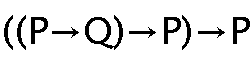
\includegraphics[scale=0.5]{pics/peirce0}}\qquad
\fbox{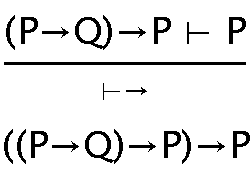
\includegraphics[scale=0.5]{pics/peirce1}}\qquad
\fbox{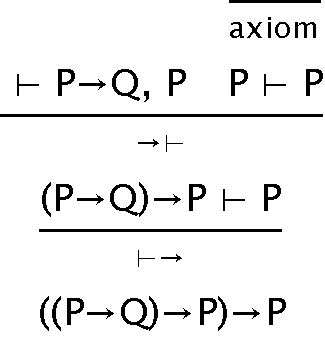
\includegraphics[scale=0.5]{pics/peirce2}}\qquad
\fbox{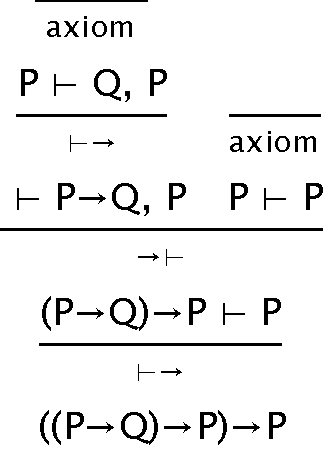
\includegraphics[scale=0.5]{pics/peirce3}}\qquad
\caption{Proof of Peirce's law by double-clicking in the multiple-conclusion sequent calculus}
\label{fig:peirce}
\end{figure}


\section{A very small example}

\Figref{peirce} shows the progress of a proof of Pierce's law in this encoding (which, you can see, is resoundingly classical).

%!TEX root = ./roll_your_own.tex
\chapter{Variations on the Sequent Calculus}
\label{chap:sequentvariations}

The calculus of \chapref{sequentcalculus} is only one of very many possible variants. In this chapter I discuss the way in which you can encode an LF-style treatment of variables in the quantifier introduction and elimination rules, how Jape deals with non-additive rules, and two versions of the intuitionistic sequent calculus --- multiple and single conclusion.

\word{var,inscope}
\begin{table}
\centering
\caption{LF variables in the multiple-conclusion sequent calculus}
\label{tab:LFvars}
\vstrut{30pt}
$\infer[\reason{(fresh $m$) ⊦∀}]
       {\Gamma |- @*x.A(x),\Delta }
       {\Gamma,\<var> m |- A(m),\Delta } $
\qquad\vstrut{30pt}
$\infer[\reason{⊦∃}]
       {\Gamma  |-|*x.A(x) ,\Delta }
       {\Gamma  |- A(B),\Delta \quad \Gamma |- B\;\<inscope>} $
\qquad\vstrut{30pt}
$\infer[\reason{∀⊦}]
       {\Gamma,@*x.A(x) |- \Delta }
       {\Gamma,A(B)  |- \Delta \quad \Gamma |- B\;\<inscope>}$
\qquad\vstrut{30pt}
$\infer[\reason{(fresh $m$) ∃⊦}]
       {\Gamma ,|*x.A(x)  |- \Delta }
       {\Gamma,\<var> m,A(m)  |- \Delta }$
\end{table}

\section{LF-style variables in quantifier rules}

Jape allows redefinition of any rule, theorem or conjecture\footnote{And it allows it \emph{at any time}!! It ought to check, whenever a rule or theorem is redefined, every proof that relies upon it. It doesn't.}. The file \texttt{examples/MSC\_LF.j} redefines the quantifier rules to allow a more careful treatment of variables\footnote{Explanation for non-expert logicians: the effect is to make it much more careful about the treatment of possibly-empty domains of quantification. It is impossible, for example, to prove $@*x.P(x) |- |*x.P(x)$, because the proof would require that there be some $m$ such that $P(m)$.}. The new rules are shown in \tabref{LFvars}.

The intention is that a variable $c$ is `$\<inscope>$' if there is an assumption $\<var> c$; a formula is $\<inscope>$ if its free variables. Note that there is nothing in Jape which demands that we use these words nor this technique: it's up to the logic decoder to program it.


The file \texttt{sequent\_scoping.j} defines two low priority prefix operators:
\begin{quote}\tt\small
PREFIX  10              var \\
POSTFIX 10              inscope
\end{quote}
and a structural induction to handle formulae,\footnote{This induction is unnecessary: in the sequent calculus we never need anything more complicated than a variable. But I wanted to see if I could do something more general, and I have left it in.} automatically applied whenever there is an open tip:
\begin{quote}\tt\small

RULES "inscope" ARE
\tab       Γ, var x ⊢ x inscope\\
AND     FROM Γ ⊢ A inscope AND Γ ⊢ B inscope INFER Γ ⊢ A→B inscope\\
AND     FROM Γ ⊢ A inscope AND Γ ⊢ B inscope INFER Γ ⊢ A∧B inscope\\
AND     FROM Γ ⊢ A inscope AND Γ ⊢ B inscope INFER Γ ⊢ A∨B inscope\\
AND     FROM Γ ⊢ A inscope INFER Γ ⊢ ¬A inscope\\
AND     FROM Γ, var x ⊢ A inscope INFER Γ ⊢ ∀x.A inscope\\
AND     FROM Γ, var x ⊢ A inscope INFER Γ ⊢ ∃x.A inscope \\
END

\end{quote}

Encoding of the rules is then straightforward in \texttt{MSC\_LF.j}:
\begin{quote}\tt\small
RULE    "⊢∀"(OBJECT m) WHERE FRESH m\\
\tab                    FROM Γ, var m ⊢ A(m),∆                    INFER Γ ⊢ ∀x.A(x),∆\\
RULE    "∀⊢"(B)   FROM Γ, A(B) ⊢ ∆ AND Γ ⊢ B inscope      INFER Γ,∀x.A(x) ⊢ ∆\\
RULE    "⊢∃"(B)   FROM Γ ⊢ A(B),∆ AND Γ ⊢ B inscope       INFER Γ ⊢ ∃x.A(x),∆\\
RULE    "∃⊢"(OBJECT m) WHERE FRESH m\\
\tab                    FROM  Γ, var m, A(m) ⊢ ∆                  INFER Γ, ∃x.A(x) ⊢ ∆\\
\end{quote}
I would like inscope judgements to behave like side conditions, displayed when they are a problem and hidden when they are satisfied. But they aren't provisos, because they relate a particular context and a particular formula.

In order to make these judgements behave like side conditions I use Jape's \textsc{layout} tactical: it allows me to run a tactic and to decide which subtrees of the resulting proof tree should be displayed and what should be written as the justification of the step. (Subtrees which contain open problem sequents are always displayed, so that nothing which might accidentally be important is hidden.) In the case of the ⊦∀ and ∃⊦ rules I would like to display the first antecedent proof (numbered 0) and hide the second (numbered 1); in either case I want to give the name of the rule as the justification of the step. The tactics are
\begin{quote}\tt\small

TACTIC "∀⊢ with side condition hidden" IS LAYOUT "∀⊢" (0) (WITHSELECTIONS "∀⊢")\\
TACTIC "⊢∃ with side condition hidden" IS LAYOUT "⊢∃" (0) (WITHSELECTIONS "⊢∃")
\end{quote}
which I put into the menu, overwriting any previous entries with the same label:
\begin{quote}\tt\small
MENU Rules IS
\tab ENTRY "∀⊢" IS "∀⊢ with side condition hidden"\\
\tab ENTRY "⊢∃" IS "⊢∃ with side condition hidden"\\
END
\end{quote}
and into the list of double-click actions
\begin{quote}\tt\small
HYPHIT  ∀x.A ⊢  IS "∀⊢ with side condition hidden"\\
CONCHIT ⊢ ∃x.B  IS "⊢∃ with side condition hidden"
\end{quote}
You get all this machinery by loading \texttt{MCS.jt}, to get the multiple-conclusion sequent calculus, and then adding \texttt{MCS\_LF.j}, to get the extra rules and syntax.

\begin{figure}
\centering
\fbox{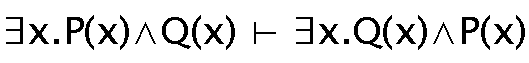
\includegraphics[scale=0.5]{pics/LF0}}\qquad
\fbox{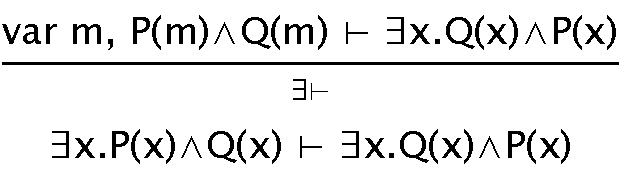
\includegraphics[scale=0.5]{pics/LF1}}\qquad
\fbox{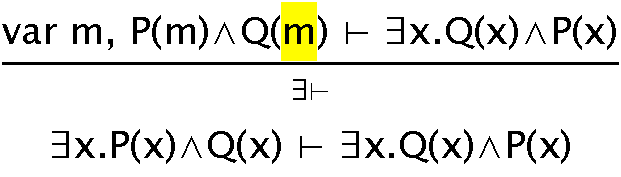
\includegraphics[scale=0.5]{pics/LF1a}}\qquad
\fbox{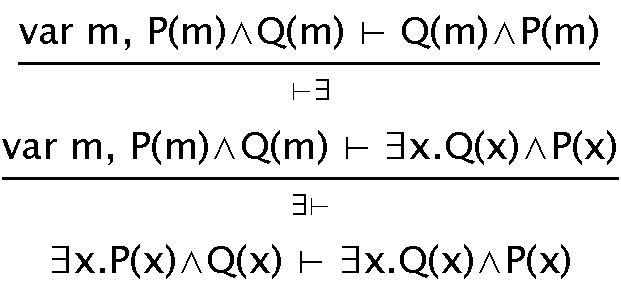
\includegraphics[scale=0.5]{pics/LF2}}\qquad
\caption{Using LF variables in the multiple-conclusion sequent calculus}
\label{fig:LF}
\end{figure}


\begin{figure}
\centering
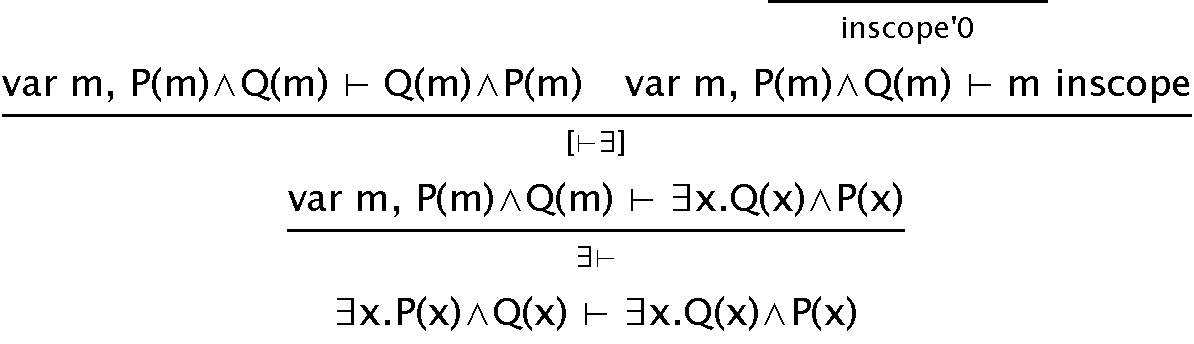
\includegraphics[scale=0.5]{pics/LF2a}
\caption{Hidden antecedents exposed}
\label{fig:LFa}
\end{figure}


Under this encoding, \figref{LF} showsthe progress of a proof in which the variable rules are obeyed. One antecedent of the final step isn't shown. You can see the full tree, shown in \figref{LFa}, by double-clicking on the justification of that step. Clearly it is an advantage to hide the side-proof whenever possible; it makes sense to hide it when it is closed, as in this case.

\begin{figure}
\centering
\fbox{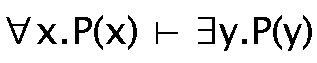
\includegraphics[scale=0.5]{pics/LFbad0}}\qquad
\fbox{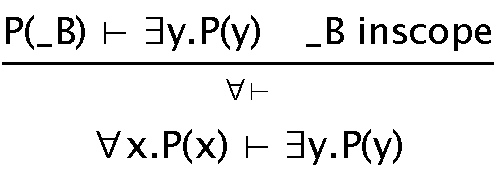
\includegraphics[scale=0.5]{pics/LFbad1}}\qquad
\fbox{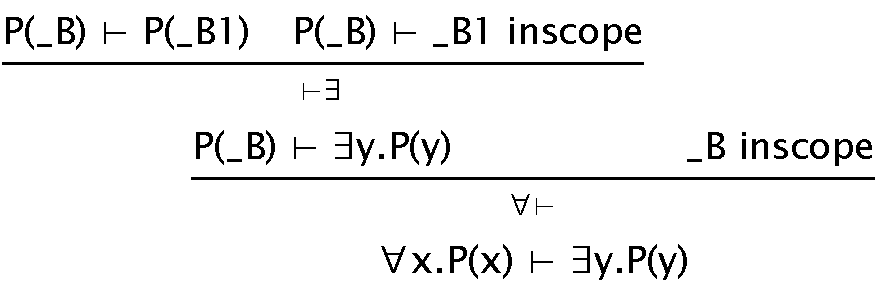
\includegraphics[scale=0.5]{pics/LFbad2}}\qquad
\caption{Not using LF variables in the multiple-conclusion sequent calculus}
\label{fig:LFbad}
\end{figure}


\Figref{LFbad} shows the progress of an attempt to prove $@*x.P(x)|-|*y.P(y)$, which isn't a theorem in this logic (though it is in the logic of \chapref{sequentcalculus}. It doesn't matter what you unify with $\_B$: the side conditions won't go away, and you can't make a theorem.

\subsection{Caveat}

A deficiency of Jape is that it has only one class of formula, but the contexts which will be built up in this encoding include logical formulae and extra-logical remarks like $\<var> c$. That would permit you, if you were actively incautious, to try to prove nonsense like $\<var> m @ \<var> n$. I don't know how to fix the problem.

\begin{table}
\centering
\caption{Intuitionistic multiple-conclusion sequent calculus rules}
\label{tab:IMCSrules}
$\infer[\reason{⊦¬}]
       {\Gamma  |- !A,\Delta }
       {\Gamma,A |- }$
\qquad\vstrut{30pt}
$\infer[\reason{⊦→}]
       {\Gamma  |- A->B,\Delta }
       {\Gamma,A |- B}$
\qquad\vstrut{30pt}
$\infer[\reason{¬⊦}]
       {\Gamma,!A |- \Delta }
       {\Gamma  |- A}$
\qquad\vstrut{30pt}
$\infer[\reason{→⊦}]
       {\Gamma,A-> B |- \Delta }
       {\Gamma  |- A & \Gamma,B |- \Delta }$\vstrut{30pt}
\end{table}

\begin{figure}
\centering
\fbox{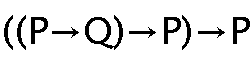
\includegraphics[scale=0.5]{pics/IMCSPeirce0}}\qquad
\fbox{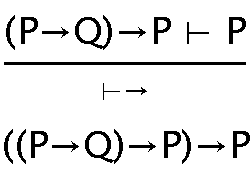
\includegraphics[scale=0.5]{pics/IMCSPeirce1}}\qquad
\fbox{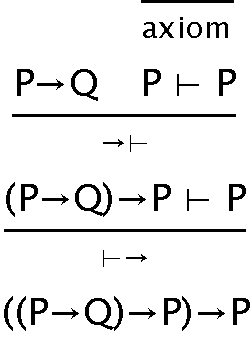
\includegraphics[scale=0.5]{pics/IMCSPeirce2}}\qquad
\caption{No Peirce's law in the intuitionistic multiple-conclusion sequent calculus}
\label{fig:IMCSPeirce}
\end{figure}


\section{The intuitionistic multiple-conclusion sequent calculus}

The rules of the intuitionistic multiple-conclusion sequent calculus aren't simply additive, but they use little more than specialised weakening. The calculus is just that of \chapref{sequentcalculus}, with different definitions of a few rules, shown in \tabref{IMCSrules}. These are defined in the file \texttt{IMCS.j}, which you can load after \texttt{MCS.jt} (and \begin{quote}\tt\small
RULE    "⊢¬"        FROM Γ,A ⊢                  INFER Γ ⊢ ¬A,∆\\
RULE    "¬⊢"        FROM Γ ⊢ A                  INFER Γ,¬A ⊢ ∆\\
RULE    "⊢→"        FROM Γ,A ⊢ B                INFER Γ ⊢ A→B,∆\\
RULE    "→⊢"        FROM Γ ⊢ A AND Γ,B ⊢ ∆   INFER Γ,A→B ⊢ ∆
\end{quote}
These definitions make it impossible to prove Pierce's law (see \figref{IMCSPeirce}), as you would expect.

\begin{table}
\centering
\caption{Multiplicative multiple-conclusion sequent calculus rules}
\label{tab:MMCSrules}
$\infer[\reason{axiom}]
       {A |- A} {}$
\qquad\vstrut{30pt}
$\infer[\reason{⊦∧}]
       {\Gamma,\Gamma' |- A@B,\Delta,\Delta' }
       {\Gamma  |- A,\Delta & \Gamma'  |- B,\Delta' }$
\qquad\vstrut{30pt}
$\infer[\reason{∨⊦}]
       {\Gamma,\Gamma' ,A|B |- \Delta,\Delta' }
       {\Gamma,A |- \Delta & \Gamma',B |- \Delta' }$
\qquad\vstrut{30pt}
$\infer[\reason{→⊦}]
       {\Gamma,\Gamma' ,A->B |- \Delta,\Delta' }
       {\Gamma  |- A,\Delta & \Gamma',B |- \Delta' }$
\qquad\vstrut{30pt}
$\infer[\reason{cut}]
       {\Gamma,\Gamma' |- \Delta,\Delta' }
       {\Gamma  |- B,\Delta & \Gamma',B |- \Delta' }$\vstrut{30pt}
\end{table}

\begin{figure}
\centering
\fbox{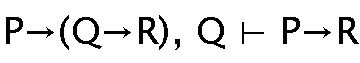
\includegraphics[scale=0.5]{pics/unifiesproviso0}}\qquad
\fbox{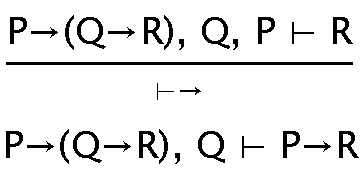
\includegraphics[scale=0.5]{pics/unifiesproviso1}}\qquad
\fbox{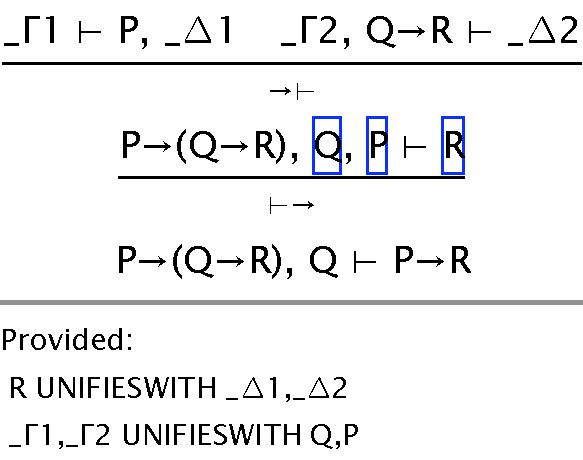
\includegraphics[scale=0.5]{pics/unifiesproviso2}}\qquad
\caption{A proof in which contexts split}
\label{fig:unifiesproviso}
\end{figure}


\begin{figure}
\centering
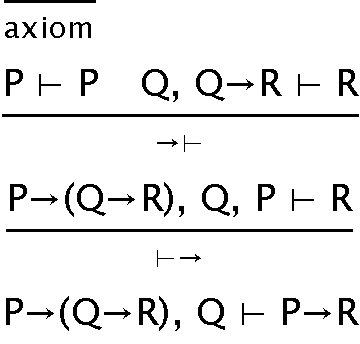
\includegraphics[scale=0.5]{pics/unifiesprovisoresolved}
\caption{Context split resolved by axiom}
\label{fig:unifiesprovisoresolved}
\end{figure}


\section{A multiple-conclusion sequent calculus with multiplicative rules}

The logic is just the normal multiple-conclusion calculus, with all of the branching rules written in multiplicative style; for maximum effect I chose an axiom rule which doesn't ignore unmatched conclusions. See \tabref{MMCSrules} for the altered rules. These rules are defined in MMCS.j, ready to be loaded after MCS.jt:
\begin{quote}\tt\small
RULE    axiom(A)                                    INFER A ⊢ A\\
RULE    "⊢∧"        FROM Γ1 ⊢ A,∆1 AND Γ2 ⊢ B,∆2        INFER Γ1,Γ2 ⊢ A∧B,∆1,∆2\\
RULE    "∨⊢"        FROM Γ1,A ⊢ ∆1 AND Γ2,B ⊢ ∆2        INFER Γ1,Γ2,A∨B ⊢ ∆1,∆2\\
RULE    "→⊢"        FROM Γ1 ⊢ A,∆1 AND Γ2,B ⊢ ∆2        INFER Γ1,Γ2,A→B ⊢ ∆1,∆2\\
RULE    "⊢≡"        FROM Γ1 ⊢ A→B,∆1 AND Γ2 ⊢ B→A,∆2  INFER Γ1,Γ2 ⊢ A≡B,∆1,∆2\\
RULE    cut(A)        FROM Γ1 ⊢ A,∆1 AND Γ2,A ⊢ ∆2        INFER Γ1,Γ2 ⊢ ∆1,∆2
\end{quote}

Since I have redefined cut, I have to redeclare its r\^{o}le to Jape:
\begin{quote}\tt\small
STRUCTURERULE CUT                   cut /* cos it's different now */
\end{quote}

When you use a multiplicative rule in this encoding, the left and right contexts split. Jape automatically records this fact in a \textsc{unifieswith} proviso, as shown in the last step of \figref{unifiesproviso}. In this simple example we have to decide whether to send $P$ and $Q$ into \_Γ1 or \_Γ2, $R$ into \_Δ1 or \_Δ2. The axiom rule of this encoding was designed to help: select $P$ in the left antecedent and apply axiom, to produce the result shown in \figref{unifiesprovisoresolved}.

\begin{figure}
\centering
\fbox{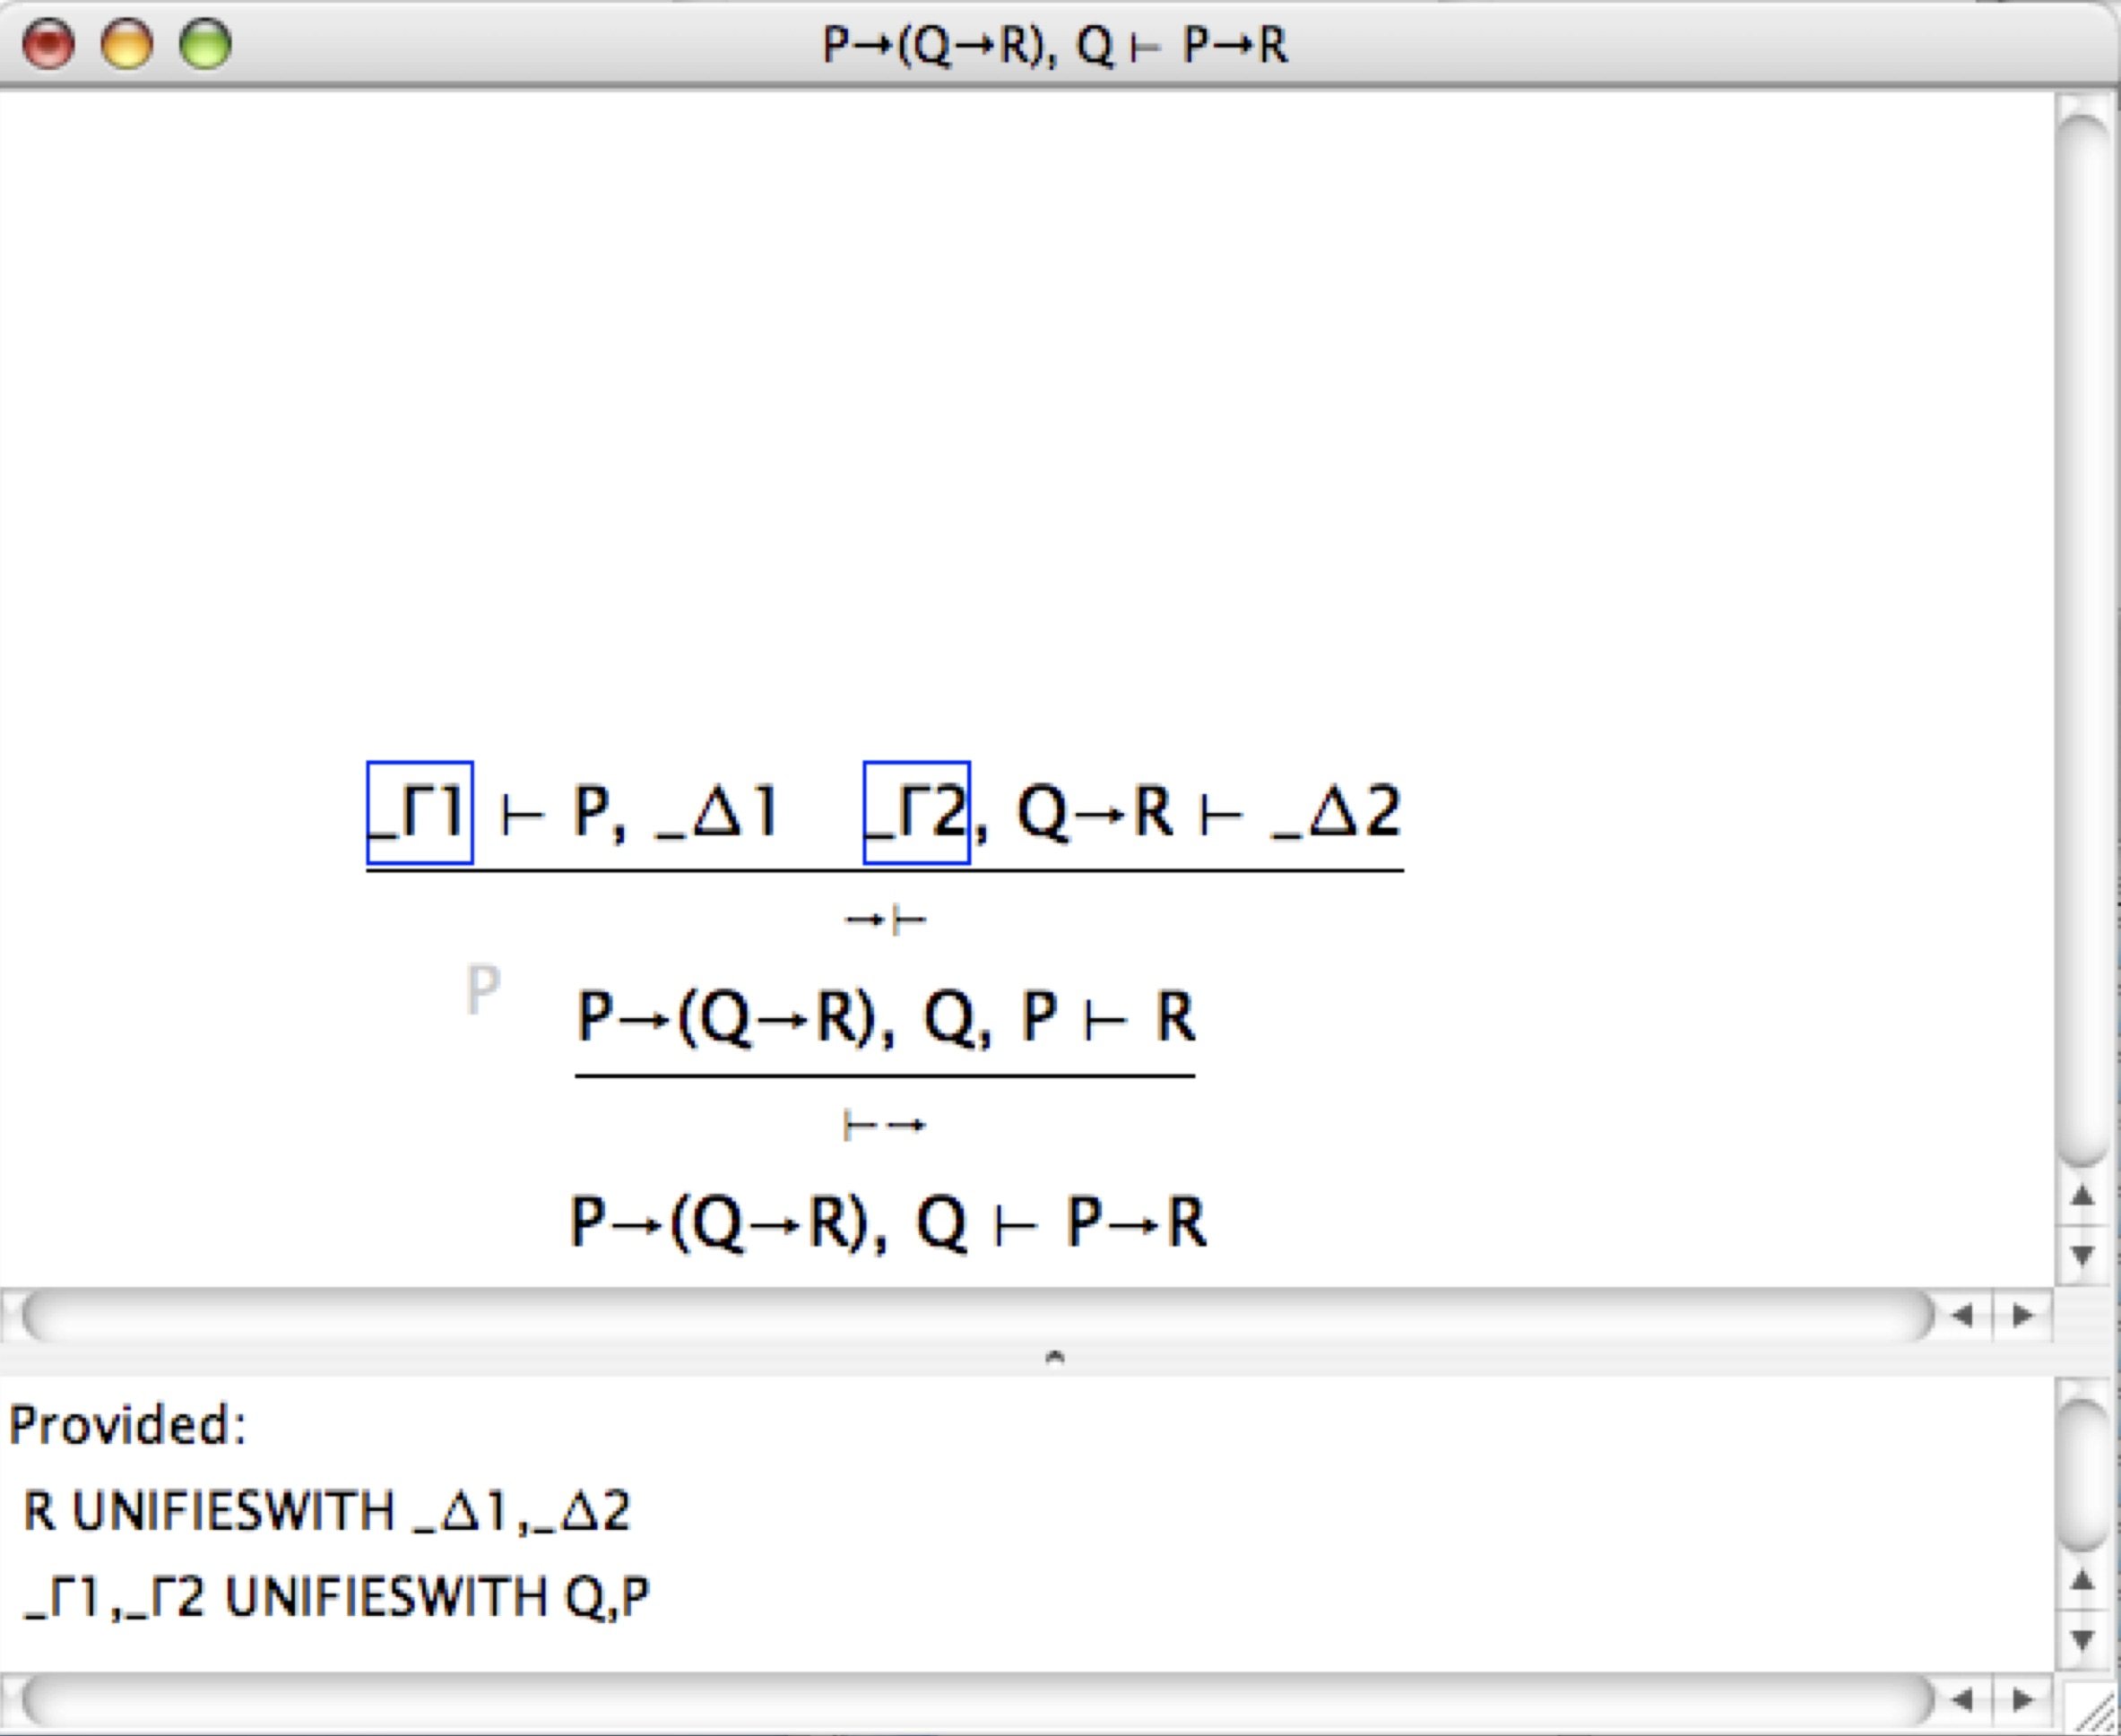
\includegraphics[scale=0.07]{pics/dragstage1.jpg}}\\
\fbox{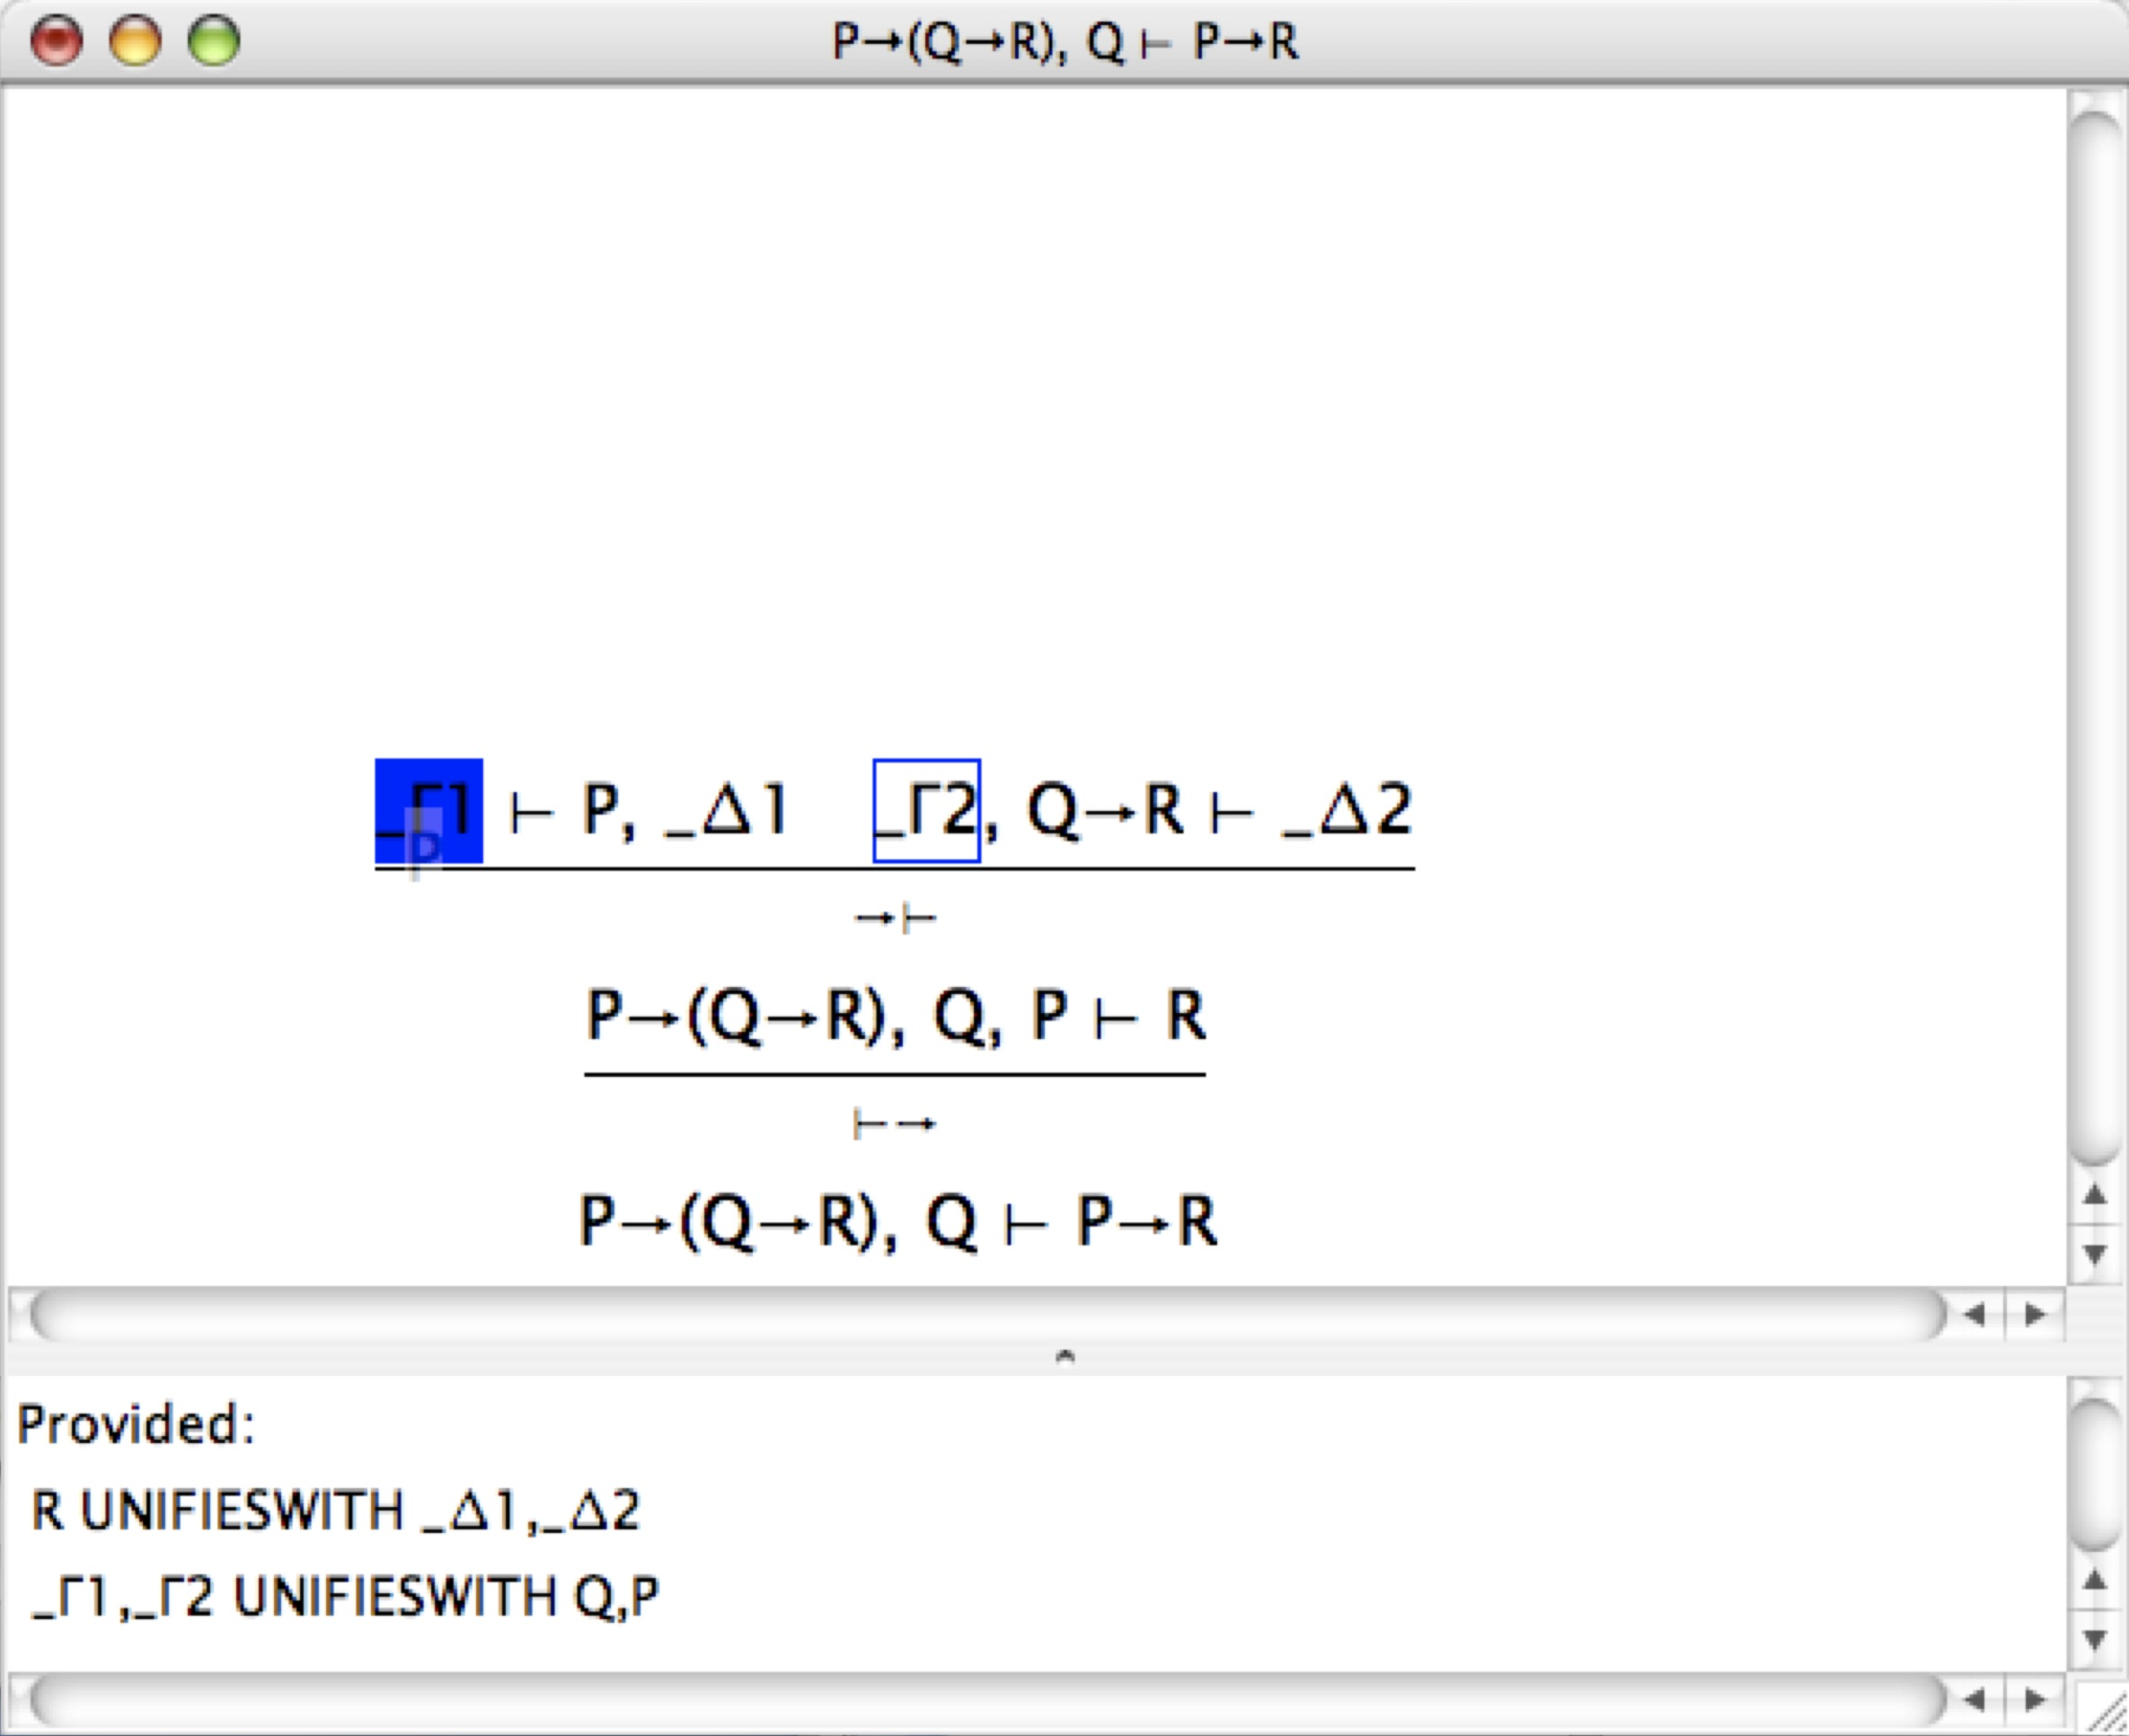
\includegraphics[scale=0.07]{pics/dragstage2.jpg}}\\
\fbox{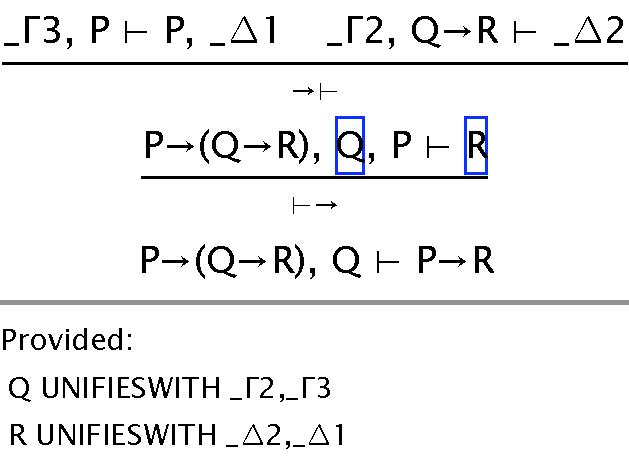
\includegraphics[scale=0.5]{pics/dragstage3}}
\caption{Resolving a context split with drag-and-drop}
\label{fig:dragstages}
\end{figure}


\textit{Resolving context-splits with drag-and-drop}

Three of the formulae in the last frame of \figref{unifiesproviso} are outlined in blue. That indicates that they are candidates for dragging into destination segment-variables. If you press and drag on the outlined instance of $P$, for example, the outlining changes to show valid drag destinations, as shown in the first frame of \figref{dragstages}. In the second frame we see how highlighting changes again when $P$ is dragged over a valid destination, and the third frame shows the effect of dropping $P$ there. Dragging $Q$ into \_Γ2 and $R$ into \_Δ2 resolves the split completely.

A similar technique can be used with rules that involve explicit weakening.


\section{Modal logic}

I intended to enhance Jape to deal with modal and linear logic. The drag-and-drop gesture, I imagined, would be part of the solution. Not so: not all the parts of a modal context split appear in the antecedents, so they wouldn't be in the proof window. And I never quite managed to wrestle the unifier into the shape it would need to deal with modal unifications. So it didn't happen as promised.


\section{Single-conclusion sequent calculus (the intuitionistic fragment)}

This was the first logic encoding that Jape ran, built by Bernard Sufrin and me in 1992. The encoding is in the file \texttt{examples/SCS.jt}.

\subsection{Inference rules}

Apart from the treatment of negation, these are a pretty ordinary selection. As with the multiple-conclusion calculus, we have chosen to use a hypothesis rule which ignores additional hypotheses, and we have made the left-hand side of a sequent a bag of formulae. The rules are very similar to those of \chapref{sequentcalculus} with Δs deleted or replaced by a formula variable $C$. In our encoding the right-hand side of a sequent contains exactly one formula --- Jape can't yet handle sequents with at most one formula on the right-hand side --- and we give rules for negation --- Jape can't yet handle definitional equality. 

Negation is often described by defining it to be equivalent to implication of absurdity: that is, $!x$ is just a way of writing $x->\bot$. Jape can't handle definitional equality, and therefore we give rules which implement that equality. The rules in \texttt{SCS\_rules.j} are
\begin{quote}\tt\small
RULE    hyp(A)                          INFER Γ,A ⊢ A\\
RULE    "⊢∧"    FROM Γ ⊢ A AND Γ ⊢ B    INFER Γ ⊢ A∧B\\
RULE    "∧⊢"    FROM Γ, A, B ⊢ C                INFER Γ, A∧B ⊢ C\\
RULE    "⊢∨(L)"     FROM  Γ ⊢ A         INFER Γ ⊢ A∨B\\
RULE    "⊢∨(R)"     FROM  Γ ⊢ B         INFER Γ ⊢ A∨B\\
RULE    "∨⊢"    FROM Γ, A ⊢ C AND Γ, B ⊢ C      INFER Γ, A∨B ⊢ C\\
RULE    "⊢¬"    FROM Γ ⊢ A→ ⊥           INFER Γ ⊢ ¬A\\
RULE    "¬⊢"    FROM Γ, A→ ⊥ ⊢ B                INFER Γ, ¬A ⊢ B\\
RULE    "⊢→"    FROM Γ, A ⊢ B           INFER Γ ⊢ A→B\\
RULE    "→⊢"    FROM Γ ⊢ A AND Γ, B ⊢ C INFER Γ, A→B ⊢ C\\
RULE    "⊢≡"    FROM Γ ⊢ A→B AND Γ ⊢ B→A        INFER Γ ⊢ A≡B\\
RULE    "≡⊢"    FROM Γ, A→B,  B→A ⊢ C   INFER Γ, A≡B ⊢ C\\
RULE    "⊥⊢"                            INFER Γ, ⊥ ⊢ A\\
RULE    "⊢∀"(OBJECT m) WHERE FRESH m\\
\tab            FROM Γ ⊢ P(m)           INFER Γ ⊢ ∀x.P(x)\\
RULE    "∀⊢"(B)     FROM Γ, P(B) ⊢ C            INFER Γ, ∀x.P(x) ⊢ C\\
RULE    "⊢∃"(B)     FROM Γ ⊢ P(B)               INFER Γ ⊢ ∃x.P(x)\\
RULE    "∃⊢"(OBJECT m) WHERE FRESH m\\
\tab              FROM  Γ, P(m) ⊢ C               INFER Γ, ∃x.P(x) ⊢ C\\
RULE    cut(A)  FROM Γ ⊢ A AND Γ, A ⊢ C INFER Γ ⊢ C\\
RULE    thin(A)     FROM Γ ⊢ B          INFER Γ, A ⊢ B\\
RULE    dup(A)  FROM Γ, A, A ⊢ B                INFER Γ, A ⊢ B
\end{quote}

\subsection{LF-style variables}

There is an encoding of an LF-style treatment of variables in the file \texttt{SCS\_LF.j}. It's identical to the treatment of variables in the multiple-conclusion calculus, with the Δ symbol deleted.

\subsection{Syntax}

Formula syntax, and use of names, is exactly as in the multiple-conclusion sequent calculus (they share the \texttt{sequent\_syntax.j} file).

Jape can't at present be configured to handle sequents with an optional formula on the right-hand side, but can deal with those with exactly one formula there. We therefore state
\begin{quote}\tt\small
SEQUENT IS BAG ⊢ FORMULA
\end{quote}

\subsection{Menus and panels}

The Rules menu is almost the same as that in the multiple-conclusion sequent calculus. The Conjectures panel is identical: the two encodings share the file \texttt{sequent\_problems.j}.

\subsection{Global variable settings}

Just as in the case of the multiple-conclusion sequent calculus, we don't want to allow the application of conjectures as if they were proved theorems and we don't want to allow the application of theorems if their hypotheses don't match.\footnote{These are pragmatic choices, driven by our expected audience of novices learning about logic. There is, of course, nothing about the logic which forces either choice.} We therefore include
\begin{quote}\tt\small
INITIALISE applyconjectures false\\
INITIALISE tryresolution false
\end{quote}

We do, however, want to allow the user to switch display modes. In place of an \textsc{initialise} directive for the \textit{displaystyle} variable, we include menu entries which control it, by inserting a radio button into the Edit menu --- one of the system menus of the Jape graphical interface. A radio button in a graphical interface is a control which has a number of mutually-exclusive settings. In a menu this appears as a number of entries, the selected one of which is ticked.
\begin{quote}\tt\small
MENU "Edit"\\
\tab RADIOBUTTON displaystyle IS\\
\tab \tab \tab "Box display"   IS box\\
\tab AND "Tree display"  IS tree\\
\tab INITIALLY tree\\
\tab END\\
END
\end{quote}
The subject of display modes is discussed in \chapref{boxNtree}.


\chapter{Display modes: box and tree}
\label{chap:boxNtree}

\begin{figure}
\begin{center}
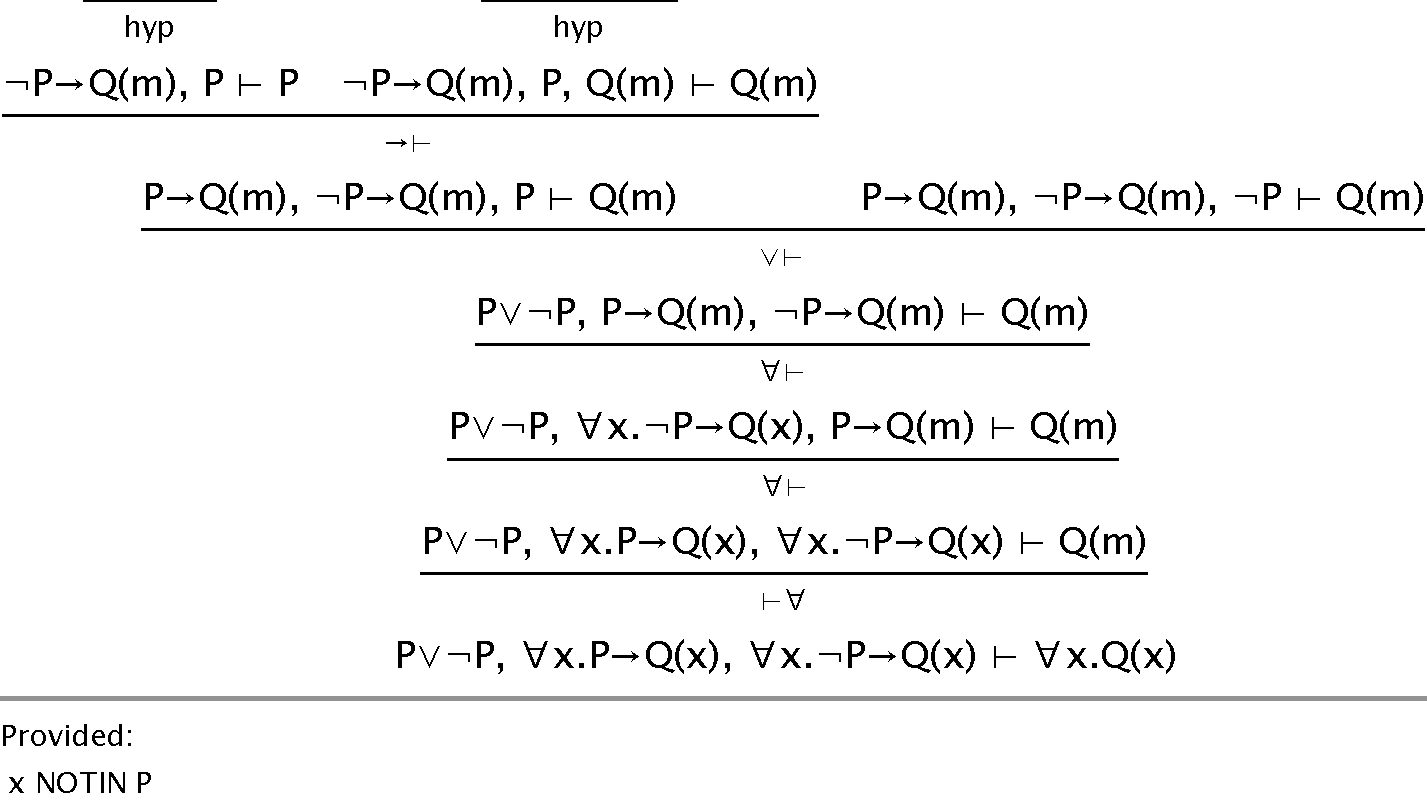
\includegraphics[scale=0.5]{pics/sampletree}
\caption{A sample proof attempt, shown as a tree}
\label{fig:sampletree}
\end{center}
\end{figure}

\begin{figure}
\begin{center}
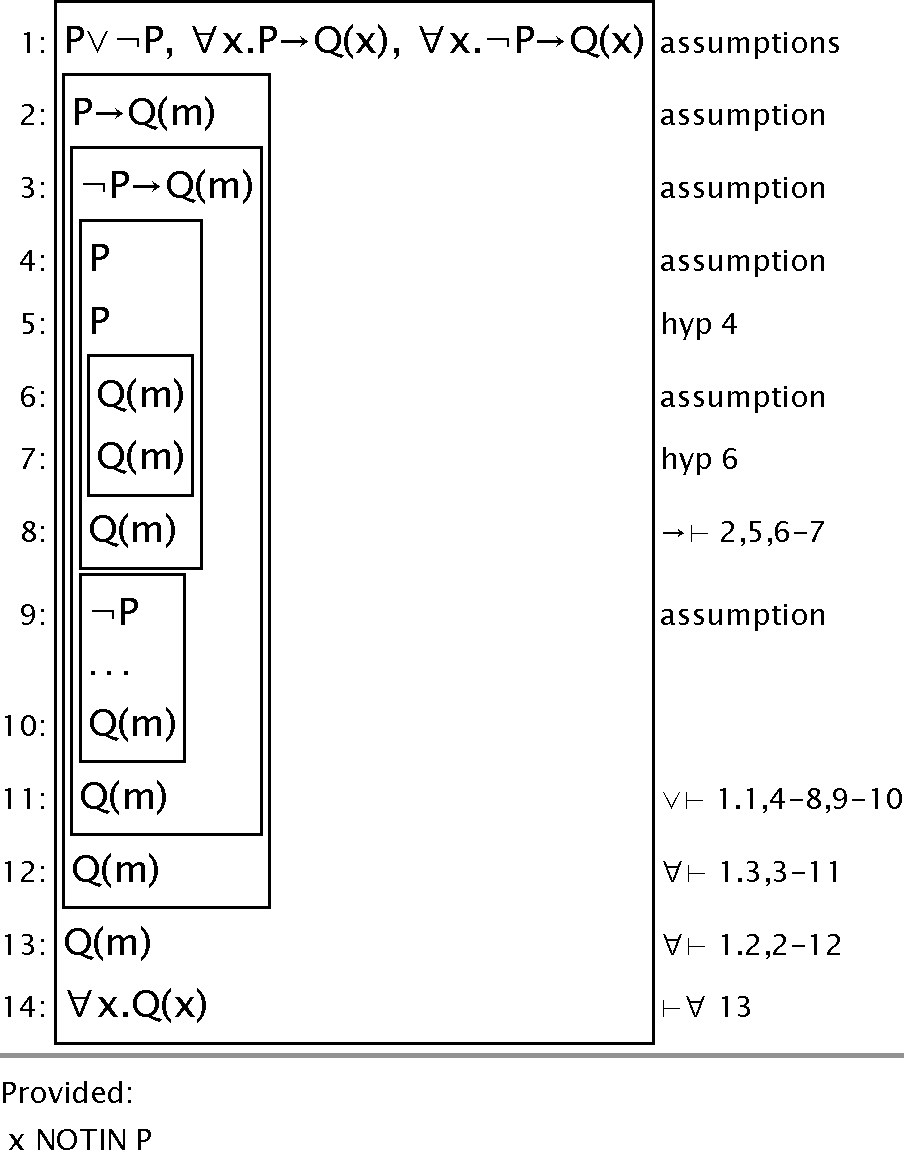
\includegraphics[scale=0.5]{pics/sampleboxNline}
\caption{A sample proof attempt, shown as box-and-line}
\label{fig:sampleboxNline}
\end{center}
\end{figure}

\begin{figure}
\begin{center}
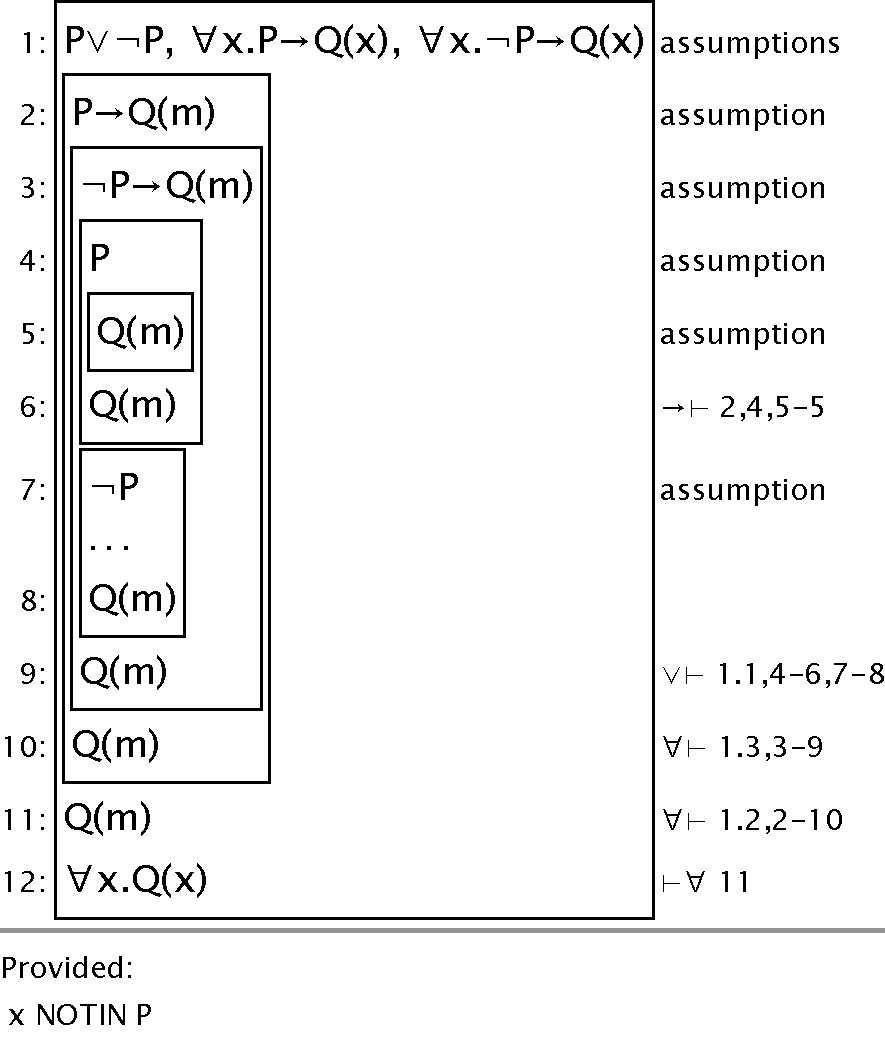
\includegraphics[scale=0.5]{pics/sampleboxNlinehiddenhyp}
\caption{A sample proof attempt, shown as box-and-line, with hidden \texttt{hyp} steps}
\label{fig:sampleboxNlinehiddenhyp}
\end{center}
\end{figure}

\Figref{sampletree} shows a sample proof attempt in the intuitionistic single-conclusion sequent calculus (see \texttt{examples/SCS.jt} and \chapref{sequentvariations}). It's a large tree, partly because the hypotheses are written out many times, once in each sequent in which they occur. The same proof attempt in box-and-line form is shown in \figref{sampleboxNline}: it's much narrower and, because it's essentially one-dimensional, easier to navigate. It shows exactly the same steps as the tree and is produced by a very simple algorithm: 
\begin{itemize}
\item to list a node list its antecedent nodes, then the consequent of the sequent;
\item if a node has more hypothesis formulae than its parent, show it as a box with the additional hypotheses on a line labelled `assumptions';
\item link a conclusion to its antecedents by giving their line number (or, if a box, their starting and finishing line numbers);
\item precede tips (unclosed nodes) with a line of three dots.
\end{itemize}
The algorithm saves a great deal of screen space. When a problem sequent has more than a few short hypotheses the tree will often be very wide, impossible to view in one piece. The box-and-line display is still readable, and it's easier to find your way around because you only have to go up and down.

The simple algorithm is only just the beginning ...

\section{Hiding \textsc{identity} steps}

There is still unnecessary business in \figref{sampleboxNline}. Line 5, for example, is proved by \texttt{hyp}. That rule, in the SCS encoding, is
\begin{quote}\tt\small
RULE hyp(A) INFER A ⊦ A
\end{quote}
It makes sense in the tree, but in the box-and-line version it's little more than an indirection. Line 8, for example, appeals to line 5 which appeals immediately and identically to line 4. When the r\^{o}le of \texttt{hyp} is declared to Jape
\begin{quote}\tt\small
STRUCTURERULE IDENTITY hyp
\end{quote}
and the \texttt{hidehyp} variable is set to \texttt{true} (its default value), then the picture changes to \figref{sampleboxNlinehiddenhyp}. The old line 8 is now line 6 and refers directly to the assumption on line 3. The proof is more compact, and easier to read. There's still tedious repetition of the conclusion $Q(m)$ in lines 5-6 and 8-11, but that is inevitable in this calculus, where left-hand-side rules transform hypotheses and copy the conclusion. \Chapref{ItL} shows how a Natural Deduction calculus, without left-hand rules, can avoid such repetition.

An \textsc{identity} step can still appear in a box-and-line proof if it is the last line of a box which has more than two lines, or the assumption line isn't a single formula which is the same as the last line.

\begin{figure}
\begin{center}
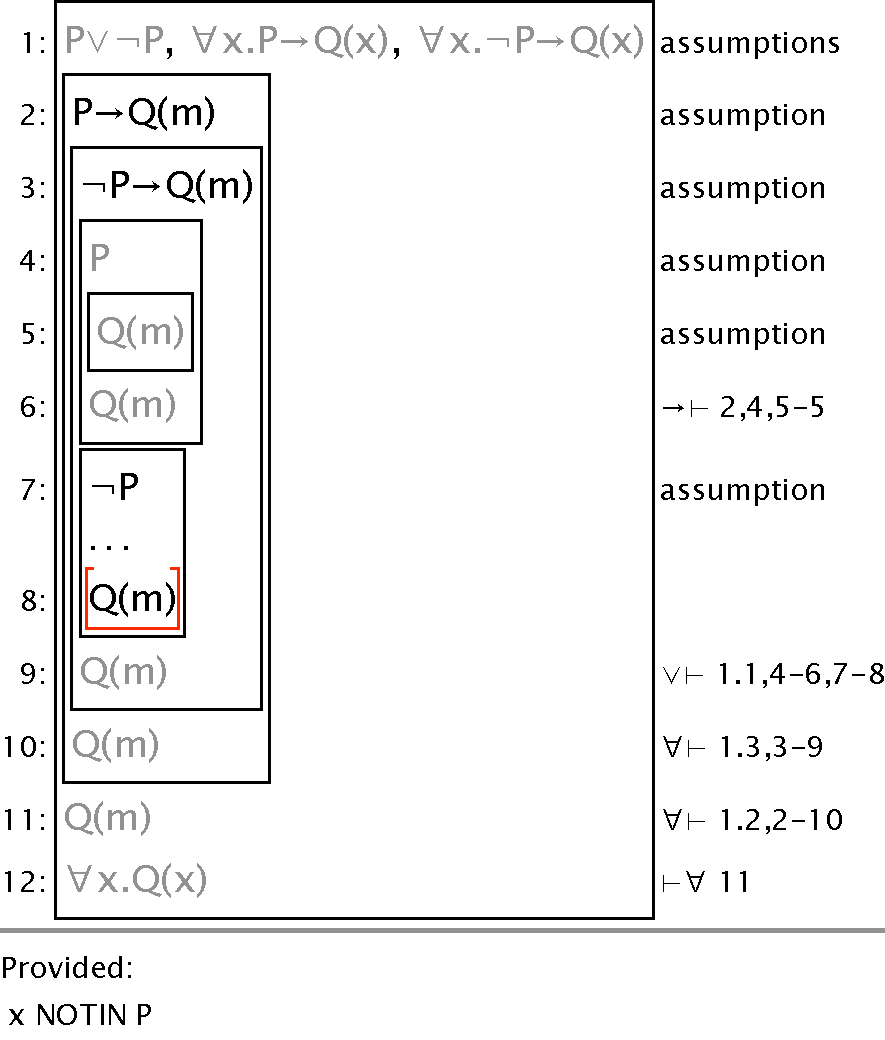
\includegraphics[scale=0.5]{pics/sampleboxNlinegreyed}
\caption{In the box-and-line presentation not all accessible formulae are usable}
\label{fig:sampleboxNlinegreyed}
\end{center}
\end{figure}

\begin{figure}
\centering
\subfigure[A bifurcated tree]{\centering
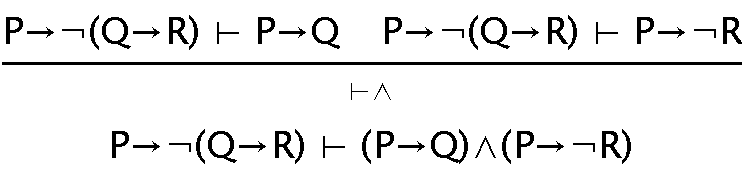
\includegraphics[scale=0.5]{pics/treebifurcated}\label{fig:treebifurcated}}
\qquad
\subfigure[Box-and-line presentation of a bifurcated tree]{\centering
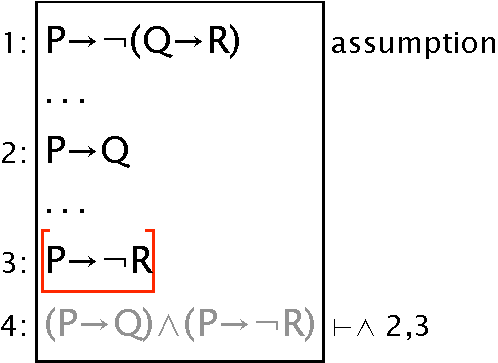
\includegraphics[scale=0.5]{pics/boxNlinebifurcated}\label{fig:boxNlinebifurcated}}
\caption{Bifurcation also causes presentation problems}
\end{figure}

\section{The tree is still there}

In \figref{sampleboxNlinehiddenhyp}, according to the rules of box-and-line proof presentation, line 8 can appeal to the assumptions on line 1, 2, 3 and 7 (it can't use line 9-12 because they are below it; it can't use lines 4-6 because they are in a box). But in the tree only $P->Q(m)$, $!P->Q(m)$ and $!P$ --- that is, lines 2, 3 and 7 --- are available. If you select the conclusion on line 8 Jape greys out all the formulae that can't be used: see \figref{sampleboxNlinegreyed}.

The effect in \figref{sampleboxNlinegreyed} is produced by left-hand rules that use up hypotheses. When a rule bifurcates the proof there are other problems. In \figref{boxNlinebifurcated}, for example, the formula on line 2 can't be selected as a hypothesis to help prove the conclusion on line 3, which breaks the normal rules of box-and-line proofs: it isn't greyed out, though, because it is possible to move the conclusion selection from line 3 to line 2. The solution to this problem is presented in \chapref{I2L}.

\section{That's not all}

Box-and-line mode, produced by setting variable \texttt{displaystyle} to \texttt{true}, can be used as an abbreviated mode of presentation of any tree proof, if you are prepared to live with the deficiencies described above. In Natural Deduction logics, without left-hand rules, it's possible to do much more, using hidden \textsc{cut} steps to produce an approximation to forward reasoning from the hypotheses (\chapref{ItL}) or, at some considerable effort, an accurate depiction (\chapref{I2L}).

\chapter{Encoding natural deduction}
\label{chap:ItL}

The sequent calculus encodings of chapters \ref{chap:sequentcalculus} and \ref{chap:sequentvariations} are each straightforward encodings of a logic, with a few directives to arrange the elements of the user interface. Natural deduction challenges us to allow forward reasoning steps. This chapter describes a first attempt: it can imitate only some kinds of forward step, and some features of the background tree are still traceable in the box display. The techniques described here are used in some later chapters, and in \chapref{I2L} a more polished attempt is described.

This encoding was used in a first-year course at QMW for several years, with increasing user satisfaction as the encoding more nearly approached the treatment used by the course lecturer. That lecturer chose the rules and, in particular, he chose to use a particular classical treatment of negation, not at all the one which I would have chosen myself, nor even the particular classical encoding which I would have preferred (see \chapref{I2L} for my own version).

The encoding is in \texttt{examples/ItL\_QMWpre2000}.

\begin{table}
\centering
\caption{Natural deduction rules in box form}
\label{tab:ItLboxrules}
\hstrut{5pt}\vstrut{5pt}\\
{\small
\begin{tabular}{|l|l|l|l|}
\hline
% ROW 1
$\begin{array}[b]{lll}
i: & A    &  \\
   & ...  &  \\
j: & A->B &  \\
   & ...  &  \\
k: & B    & \reason{$->-E\ i,j$}
\end{array}$
& 
$\begin{array}[b]{lll}
i: & A@B &  \\
   & ... &  \\
j: & A   & \reason{$@-E(L)\ i$}
\end{array}$
& 
$\begin{array}[b]{lll}
i: & A@B &  \\
   & ... &  \\
j: & B   & \reason{$@-E(R)\ i$}
\end{array}$
&
$\begin{array}[b]{lll}
i: & !!A &  \\
   & ... &  \\
j: & A   & \reason{$! -E\ i$}
\end{array}$
\\
\hline
\multicolumn{2}{|l|}{
$\begin{array}[b]{lll}
i: & A|B &  \\
   & ... &  \\
\begin{array}{@{}l}
j: \\
   \\
k:
\end{array}
		& 
		\begin{array}{|l|}
		\hline
		A \\
		... \\
		C \\
		\hline
		\end{array}
				& 
				\begin{array}{@{}l}
				\reason{assumption} \\
				\\
				\hstrut{5pt}
				\end{array}
\\
    & ... &  \\
\begin{array}{@{}l}
l: \\
   \\
m:
\end{array}
		& 
		\begin{array}{|l|}
		\hline
		B \\
		... \\
		C \\
		\hline
		\end{array}
				& 
				\begin{array}{@{}l}
				\reason{assumption} \\
				\\
				\hstrut{5pt}
				\end{array}
\\
   & ... &  \\
n: & C & \reason{$| -E\ i,j..k,l..m$}
\end{array}$}
&& \\
%ROW 3
\hline
\multicolumn{2}{|l|}{
$\begin{array}[b]{lll}
\begin{array}{@{}l}
\\
i: \\
\\
j: \\
\hstrut{5pt}
\end{array}
		& 
		\begin{array}{|l|}
		\hline
		... \\
		@*x.P(x) \\
		... \\
		P(c) \\
		... \\
		\hline
		\end{array}^{\;c}
				& 
				\begin{array}{@{}l}
				\\
				\hstrut{5pt} \\
				\\
				\reason{$@*-E\ i$} \\
				\hstrut{5pt}
				\end{array}
\end{array}$}
& 
\multicolumn{2}{|l|}{
$\begin{array}[b]{lll}
i: &|*x.P(x) &  \\
   & ... &  \\
\begin{array}{@{}l}
j: \\
\\
k:
\end{array}
		&
		\begin{array}{|l|}
		\hline
		P(c) \\
		... \\
		A \\
		\hline
		\end{array}^{\;c}
				& 
				\begin{array}{@{}l}
				\reason{assumption} \\
				\\
				\hstrut{5pt}
				\end{array}
\\
   & ... &  \\
l: & A & \reason{$|*-E\ i,j..k$}
\end{array}$}
\\
% ROW 4
\hline
\multicolumn{2}{|l|}{
$\begin{array}[b]{lll}
\begin{array}{@{}l}
i: \\
\\
j:
\end{array}
		& 
		\begin{array}{|l|}
		\hline
		A \\
		... \\
		B \\
		\hline
		\end{array}
				& 
				\begin{array}{@{}l}
				\reason{assumption} \\
				\\
				\hstrut{5pt}
				\end{array}
\\
   & ...  & \\
k: & A->B & \reason{$->-I\ i..j$} 
\end{array}$}
& 
\multicolumn{2}{|l|}{
$\begin{array}[b]{lll}
\begin{array}{@{}l}
i: \\
\\
j:
\end{array}
		& 
		\begin{array}{|l|}
		\hline
		A \\
		... \\
		B@!B \\
		\hline
		\end{array}
				& 
				\begin{array}{@{}l}
				\reason{assumption} \\
				\\
				\hstrut{5pt}
				\end{array}
\\
   & ... &  \\
k: & !A  & \reason{¬-I $i$..$j$}
\end{array}$}
\\
\hline
% ROW 5
$\begin{array}[b]{lll}
i: & A &  \\
& ... &  \\
j: & B &  \\
& ... &  \\
k: & A@B & \reason{$@-I\ i,j$}
\end{array}$
& 
$\begin{array}[b]{lll}
i: & A &  \\
& ... &  \\
j: & A|B & \reason{$| -I(L)\ i$}
\end{array}$
& 
$\begin{array}[b]{lll}
i: & B &  \\
& ... &  \\
j: & A|B & \reason{$| -I(R)\ i$}
\end{array}$
& \\
\hline
%ROW 6
\multicolumn{2}{|l|}{
$\begin{array}[b]{lll}
\begin{array}{@{}l}
\\
i:
\end{array}
		&
		\begin{array}{|l|}
		\hline
		... \\
		P(c) \\
		\hline
		\end{array}^{\;c}
				& 
\\
   & ...      &  \\
j: & @*x.P(x) & \reason{$@*-I\ i$} 
\end{array}$}
& 
\multicolumn{2}{|l|}{
$\begin{array}[b]{lll}
\begin{array}{@{}l}
\\
i: \\
\\
j: \\
\hstrut{5pt}
\end{array}
		& 
		\begin{array}{|l|}
		\hline
		... \\
		P(c) \\
		... \\
		|*x.P(x)) \\
		... \\
		\hline
		\end{array}^{\;c}
				& 
				\begin{array}{@{}l}
				\\
				\hstrut{5pt} \\
				\\
				\reason{$|*-I\ i$} \\
				\hstrut{5pt}
				\end{array}
\end{array}$}
\\
\hline
\end{tabular}
}
\end{table}

\newcommand{\vdotted}[1]{\begin{array}[b]{c}\vdots\\#1\end{array}}
\newcommand{\hvdotted}[2]{\begin{array}[b]{c}[#1]\\\vdots\\#2\end{array}}
\word{var,inscope}

\begin{table}
\centering
\caption{Natural deduction rules in tree form}
\label{tab:ItLtreerules}
\hstrut{5pt}\vstrut{5pt}\\
{\small
\begin{tabular}{|l|l|l|l|}
%ROW 0
\hline
\multicolumn{4}{|l|}{
$\infer[\reason{$hyp$}]
       {A}
       {}$}
\\
\hline
% ROW 1
$\infer[\reason{$->-E$}]
       {B}
       {\vdotted{A} \vdotted{A->B}}$
& 
$\infer[\reason{$@-E(L)$}]
       {A}
       {\vdotted{A@B}}$
& 
$\infer[\reason{$@-E(R)$}]
       {B}
       {\vdotted{A@B}}$
& 
$\infer[\reason{$\;!-E$}]
       {A}
       {\vdotted{!!A}}$
\\
\hline
\multicolumn{2}{|l|}{
$\infer[\reason{$| -E$}]
       {C}
       {\vdotted{A|B} & \hvdotted{A}{C} & \hvdotted{B}{C}}$}
&
\multicolumn{2}{|l|}{
$\infer[\reason{$@*-E$}]
       {P(c)}
       {\vdotted{@*x.P(x)} & c\;\<inscope>}$}
\\
\hline
% ROW 2
\multicolumn{4}{|l|}{
$\infer[\reason{(\textsc{fresh} $c$, $c$ \textsc{notin} $|*x.P(x)$) $|*-E$}]
       {A}
       {\vdotted{|*x.P(x)} & \hvdotted{\<var> c,P(c)}{A}}$}
\\
\hline
% ROW 3
$\infer[\reason{$->-I$}]
       {A->B}
       {\hvdotted{A}{B}}$
& 
$\infer[\reason{$@-I$}]
       {A@B}
       {\vdotted{A} & \vdotted{B}}$
& 
$\infer[\reason{$| -I(L)$}]
       {A|B}
       {\vdotted{A}}$
& 
$\infer[\reason{$| -I(R)$}]
       {A|B}
       {\vdotted{B}}$
\\
\hline 
% ROW 4
$\infer[\reason{$!-I$}]
       {!A}
       {\hvdotted{A}{B@!B}}$
&
$\infer[\reason{(\textsc{fresh} $c$) $@*-I$}]
       {@*x.P(x)}
       {\hvdotted{\<var> c}{P(c)}}$
& 
\multicolumn{2}{|l|}{
$\infer[\reason{$|*-I$}]
       {|*x.P(x)}
       {\vdotted{P(c)} & c\;\<inscope>}$}
\\
\hline
\end{tabular}}
\end{table}

\begin{table}
\centering
\caption{Natural deduction rules in sequent form}
\label{tab:ItLsequentrules}
\hstrut{5pt}\vstrut{5pt}\\
{\small
\begin{tabular}{|l|l|l|l|}
\hline
% ROW 0
\multicolumn{4}{|l|}{
$\infer[\reason{$hyp$}]
       {\Gamma,A |- A}
       {}$}
\\
\hline
% ROW 1
$\infer[\reason{$
\;->-E$}]
       {\Gamma  |- B}
       {\Gamma  |- A & \Gamma  |- A->B}$
& 
$\infer[\reason{$@-E(L)$}]
       {\Gamma  |- A}
       {\Gamma  |- A@B}$
& 
$\infer[\reason{$@-E(R)$}]
       {\Gamma  |- B}
       {\Gamma  |- A@B}$
& 
$\infer[\reason{$! -E$}]
       {\Gamma  |- A}
       {\Gamma  |- !!A}$
\\
\hline
% ROW 2
\multicolumn{2}{|l|}{
$\infer[\reason{$| -E$}]
       {\Gamma |- C}
       {\Gamma |- A|B & \Gamma,A |- C & \Gamma,B |- C}$}
& 
\multicolumn{2}{|l|}{
$\infer[\reason{$@* -E$}]
       {\Gamma  |- A(c) }
       {\Gamma  |- @*x.A(x)  & \Gamma |- c\;\<inscope>}$} 
\\ 
\hline
% ROW 3
\multicolumn{4}{|l|}{
$\infer[\reason{(\textsc{fresh} $c$, $c$ \textsc{notin} $|*x.A$) $|* -E$}]
       {\Gamma  |- B}
       {\Gamma  |-|*x.A(x)  & \Gamma ,\<var> c,A(c)  |- B}$
}
\\
\hline
% ROW 4
$\infer[\reason{$-> -I$}]
       {\Gamma  |- A->B}
       {\Gamma,A |- B}$
& 
$\infer[\reason{$@ -I$}]
       {\Gamma  |- A@B}
       {\Gamma  |- A & \Gamma  |- B}$
& 
$\infer[\reason{$| -I(L)$}]
       {\Gamma  |- A|B}
       {\Gamma  |- A}$
& 
$\infer[\reason{$| -I(R)$}]
       {\Gamma  |- A|B}
       {\Gamma  |- B}$
\\
\hline
% ROW 5 
$\infer[\reason{$\;!-I$}]
       {\Gamma  |- !A}
       {\Gamma,A |- B@!B}$
&
$\infer[\reason{(\textsc{fresh} $c$) ∀-I}]
       {\Gamma |- @*x.A(x) }
       {\Gamma,\<var> c |- A(c) }$
& 
$\infer[\reason{∃-I}]
       {\Gamma |-|*x.A(x) }
       {\Gamma  |- A(c)  & c\;\<inscope>}$
&\\
\hline
\end{tabular}}
\end{table}

\section{Inference rules}

The rules of natural deduction are not normally stated in terms of sequents. The rules were presented to me in box-and-line form as in \tabref{ItLboxrules} (there was also a reiteration rule, which I don't list).\footnote{If anybody knows how to make Latex lay out this table with adequate space before and after each row, and without picking some elements and jamming them up against the top of the box, please let me know.} The marginal $c$ in the ∃-E and ∀-I rules indicates a proviso that $c$ should not appear free outside the `scope box' which it labels; there's a corresponding condition on ∃-I and ∀-E that $c$ should be `well scoped' --- that is, lines $i$ to $j$ have to be inside a scope box for $c$.

These rules have well-known tree equivalents shown in \tabref{ItLtreerules}, where reiteration is replaced by a hypothesis rule, the provisos are made explicit and the ∃-I and ∀-E rules have an explicit side-condition. The provisos on ∃-E and ∀-I implement the provisos on the box rules reasonably accurately. They aren't quite the same, because there could be disjoint parts of the tree where the same name is used; in practice, because my encoding of these rules makes them introduce names new to the proof, the distinction is unnoticeable. To implement the condition on ∃-I and ∀-E I have used pseudo-predicates var and inscope; $c$ inscope is a side condition that var $c$ must occur in the hypotheses.

It's easy to recast these rules in sequent notation as in \tabref{ItLsequentrules}. Plainly it is a difficulty, in a backwards-reasoning tool, that these are all right-hand rules. Yet if we are to be satisfy to our client's requirements, these are the rules that we must encode. In order to understand how to do that, it is necessary to understand how they are intended to be used.

\section{Syntax (\texttt{ItL\_syntax.j})}

The description of the syntax differs only slightly from that used in the sequent calculus encodings of chapters \ref{chap:sequentcalculus} and \ref{chap:sequentvariations}. Quantification affects the \textit{smallest} following formula: that is, in this encoding $@*x.A->B$ should parse as $(@*x.A) ->B$.\footnote{Our customer also wanted no punctuation between bound variable and body: I've never found a way to make Jape's parser generator allow that.} The priority of quantification is therefore just less than that of negation.
\begin{quote}\tt\small
CLASS VARIABLE x y z c d \\
CLASS FORMULA A B C P Q R S \\
CLASS BAG FORMULA Γ \\

PREFIX  10      var \\
POSTFIX 10      inscope \\

INFIX       100R    → \\
INFIX       120L        ∨ \\
INFIX       140L        ∧ \\

LEFTFIX 180     ∀ . \\
LEFTFIX 180     ∃ . \\

PREFIX  200     ¬ \\
JUXTFIX 300 \\
SUBSTFIX    400  \\

BIND x SCOPE P IN ∀x . P \\
BIND x SCOPE P IN ∃x . P \\

SEQUENT IS BAG ⊢ FORMULA
\end{quote}

We set two variables (really they are parameters, because they can only be altered when the rule and theorem store is empty):
\begin{quote}\tt\small
INITIALISE autoAdditiveLeft true \\
INITIALISE interpretpredicatesbtrue
\end{quote}

The first of these allows us to define rules without mentioning a left context, automatically inserting a context variable \ensuremath{\Gamma} into every sequent in a rule definition (that is, allowing rule definition in the style of natural deduction and earlier versions of Jape). The second directs Jape to interpret every juxtaposition --- everything that looks like a predicate application --- as a predicate application, to translate where necessary into substitution notation and to include additional rule parameters and invisible provisos to support the translation.

\section{The rules in Japeish (\texttt{ItL\_rules.j})}

The introduction and elimination rules are exactly those of \tabref{ItLsequentrules}, all stated without repetition of the context Γ. \texttt{hyp} is \textsc{automatch}ed and an \textsc{identity} rule, just as in the sequent calculus.
\begin{quote}\tt\small
RULE "→-E"(A)      IS FROM A AND A→B INFER B \\
RULE "∧-E(L)"(B)   IS FROM A ∧ B INFER A \\
RULE "∧-E(R)"(A)   IS FROM A ∧ B INFER B \\
RULE "∨-E"(A,B)    IS FROM A ∨ B AND A ⊢ C AND B ⊢ C INFER C \\
RULE "¬-E"         IS FROM ¬¬A INFER A \\
RULE "∀-E"(c)      IS FROM ∀x. A(x) AND c inscope INFER A(c) \\
RULE "∃-E"(OBJECT c) WHERE FRESH c AND c NOTIN ∃x.A(x) \\
\tab IS FROM ∃x.A(x) AND var c, A(c) ⊢ C INFER C

RULE "→-I"         IS FROM A ⊢ B INFER A→B \\
RULE "∧-I"         IS FROM A AND B INFER A ∧ B \\
RULE "∨-I(L)"(B)   IS FROM A INFER A ∨ B \\
RULE "∨-I(R)"(A)   IS FROM B INFER A ∨ B \\
RULE "¬-I"(B)      IS FROM A ⊢ B ∧ ¬B INFER ¬A \\
RULE "∀-I"(OBJECT c) WHERE FRESH c \\
\tab IS FROM var c ⊢ A(c) INFER ∀x .A(x) \\
RULE "∃-I"(c)      IS FROM A(c) AND c inscope INFER ∃x.A(x) \\

RULE hyp(A) IS INFER A ⊢ A \\
AUTOMATCH hyp \\
STRUCTURERULE IDENTITY   hyp
\end{quote}

To imitate forward reasoning we need a \textsc{cut} rule; to use theorems easily we need a \textsc{weaken} rule.
\begin{quote}\tt\small
RULE cut(B) IS FROM B AND B ⊢ C INFER C \\
RULE thin(A) IS FROM C INFER A ⊢ C

STRUCTURERULE CUT        cut \\
STRUCTURERULE WEAKEN     thin
\end{quote}

To deal with variables we need a rule that picks up $\<var>$ declarations, and it's \textsc{automatch}ed too.
\begin{quote}\tt\small
RULE "inscope" IS INFER var x ⊢ x inscope \\
AUTOMATCH "inscope"
\end{quote}
(It is offensive to use the context in this way, as if $\<var> c$ was a logical assertion. Jape doesn't have structured contexts, more's the pity.)

\section{Variable settings (\texttt{ItL.jt})}

We don't want novices to apply a conjecture until it is proved, and we don't want the engine to use a resolution step unless a tactic commands it:
\begin{quote}\tt\small
INITIALISE applyconjectures false\\
INITIALISE tryresolution false
\end{quote}
The display style should be box-and-line, and we want to control the naming of assumptions: the outermost assumption should be ``premise'', plural ``premises'' (the \texttt{innerassumption} settings look like a hangover from an earlier version of Jape, as those are the defaults anyway):
\begin{quote}\tt\small
INITIALISE displaystyle box

INITIALISE outerassumptionword premise\\
INITIALISE outerassumptionplural premises\\
INITIALISE innerassumptionword assumption\\
INITIALISE innerassumptionplural assumptions
\end{quote}

\begin{figure} 
\centering 
\subfigure[problem statement]{\centering
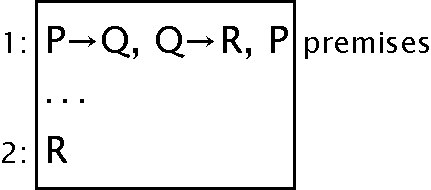
\includegraphics[scale=0.5]{pics/forwardstepA} \label{fig:forwardstepA}} 
\quad
\subfigure[hypothesis selected]{\centering
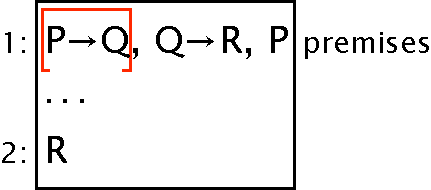
\includegraphics[scale=0.5]{pics/forwardstepB} \label{fig:forwardstepB}} 
\quad
\subfigure[after →-E]{\centering
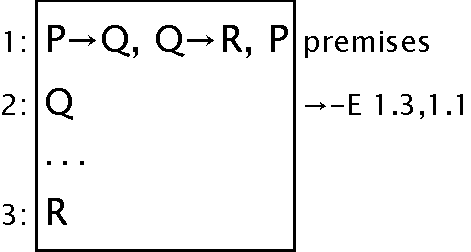
\includegraphics[scale=0.5]{pics/forwardstepC} \label{fig:forwardstepC}} 
\quad
\subfigure[second hypothesis selection]{\centering
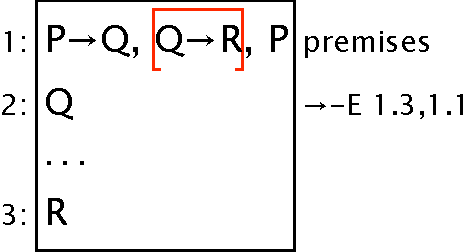
\includegraphics[scale=0.5]{pics/forwardstepD} \label{fig:forwardstepD}} 
\quad
\subfigure[second →-E completes proof]{\centering
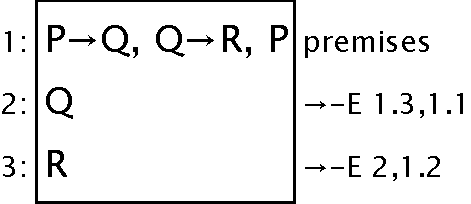
\includegraphics[scale=0.5]{pics/forwardstepE} \label{fig:forwardstepE}} 
\caption{A proof using forward steps}
\label{fig:forwardstep}
\end{figure}

\begin{figure} 
\centering 
\subfigure[after →-E]{\centering
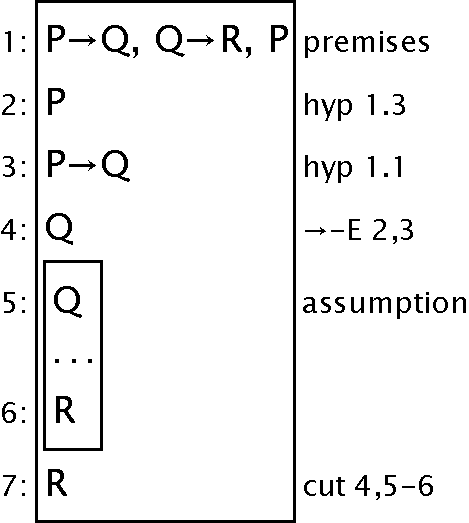
\includegraphics[scale=0.5]{pics/forwardstepwithcutC} \label{fig:forwardstepwithcutC}} 
\quad
\subfigure[tree after →-E]{\centering
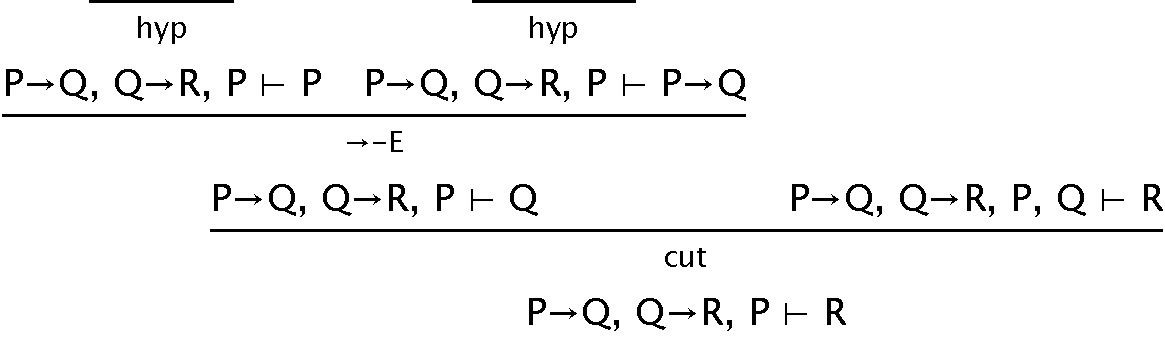
\includegraphics[scale=0.5]{pics/treeforwardstepwithcutC} \label{fig:treeforwardstepwithcutC}} 
%\quad
%\subfigure[after second →-E]{\centering
%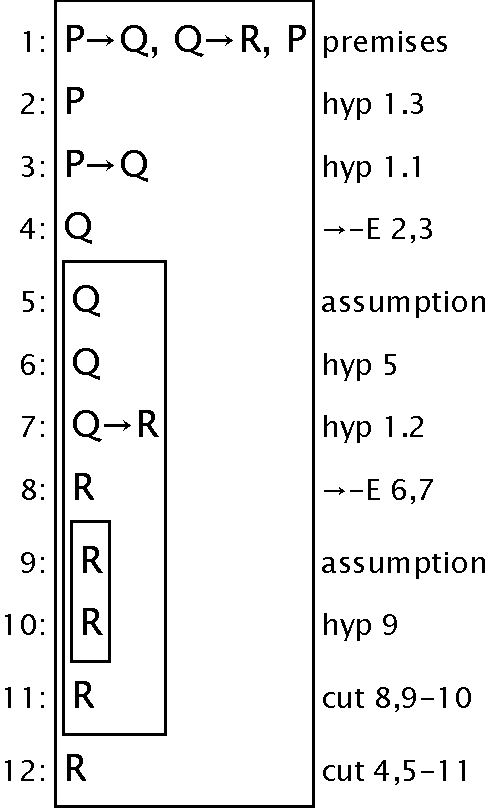
\includegraphics[scale=0.5]{pics/forwardstepwithcutE} \label{fig:forwardstepwithcutE}} 
%\quad
%\subfigure[tree after second →-E]{\centering
%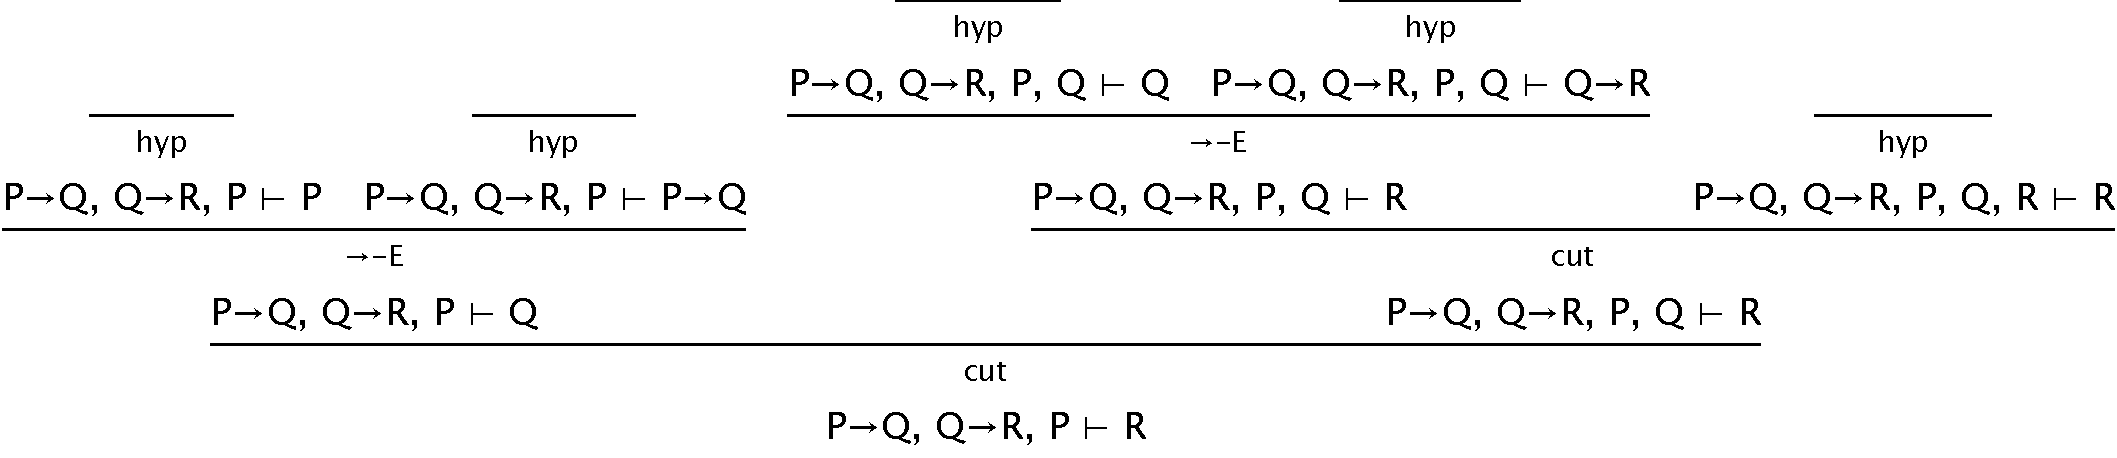
\includegraphics[scale=0.5]{pics/treeforwardstepwithcutE} \label{fig:treeforwardstepwithcutE}} 
\caption{A proof using forward steps, showing \texttt{cut} and \texttt{hyp}}
\label{fig:forwardstepwithcut}
\end{figure}

\begin{figure} 
\centering 
\subfigure[the problem]{\centering
\fbox{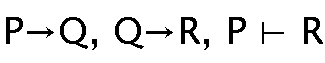
\includegraphics[scale=0.5]{pics/forwardstepslowlyA}} \label{fig:forwardstepslowlyA}} 
\quad
\subfigure[after \texttt{cut}, with unknown $\_B$]{\centering
\fbox{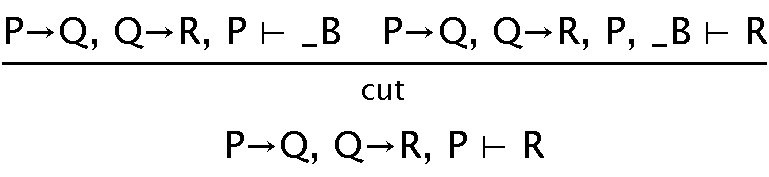
\includegraphics[scale=0.5]{pics/forwardstepslowlyB}} \label{fig:forwardstepslowlyB}} 
\quad
\subfigure[after →-E, with unknowns $\_A$ and $\_B$]{\centering
\fbox{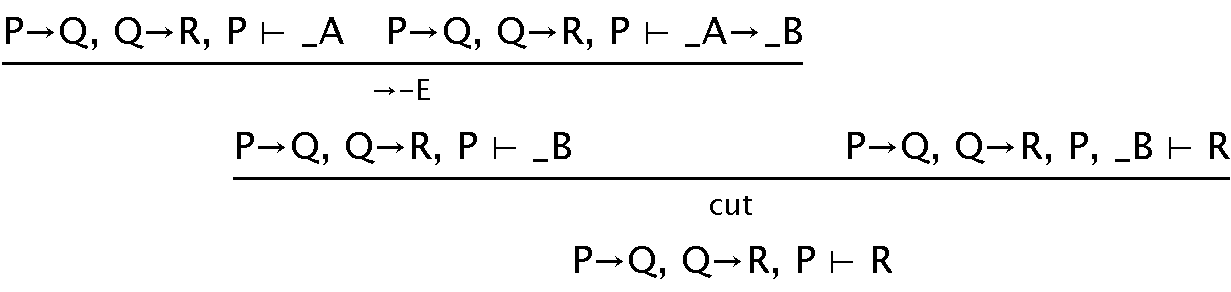
\includegraphics[scale=0.5]{pics/forwardstepslowlyC}} \label{fig:forwardstepslowlyC}} 
\quad
\subfigure[after first \texttt{hyp} (from user selection)]{\centering
\fbox{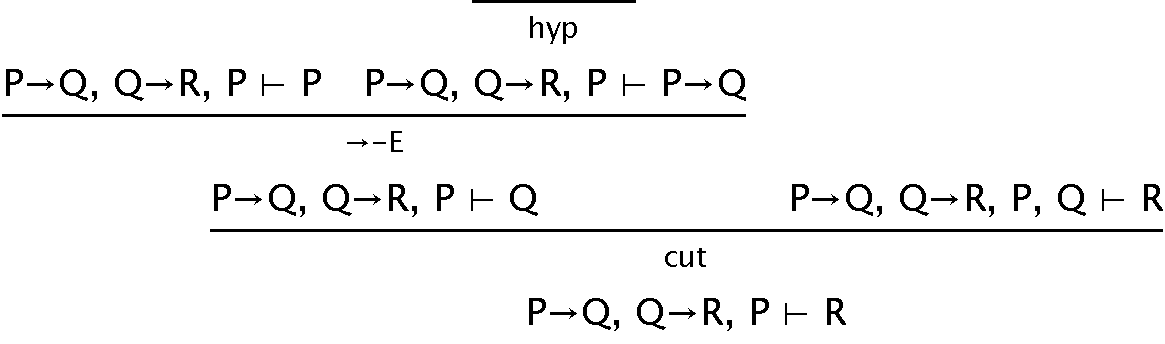
\includegraphics[scale=0.5]{pics/forwardstepslowlyD}} \label{fig:forwardstepslowlyD}} 
\quad
\subfigure[after second \texttt{hyp} (by \textsc{automatch})]{\centering
\fbox{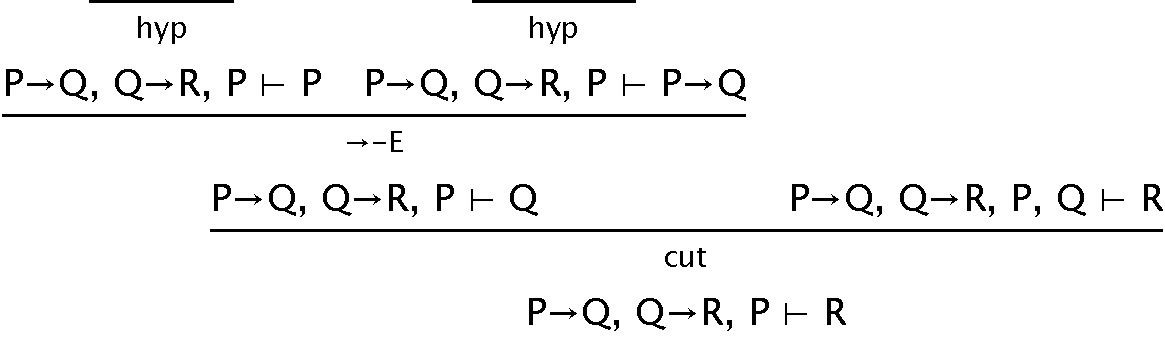
\includegraphics[scale=0.5]{pics/forwardstepslowlyE}} \label{fig:forwardstepslowlyE}} 
\caption{Stages of a sample `forward step'}
\label{fig:forwardstepslowly}
\end{figure}

\section{Forward reasoning with \texttt{cut}}

The sort of steps that a natural-deduction reasoner might want to make is best illustrated by example. Consider the problem of proving $P->Q, Q->R, P |- R$, the second problem in the Conjectures panel defined in \texttt{ItL\_problems.j}. \Figref{forwardstepA} shows the initial display; \ref{fig:forwardstepB} the first selection; \ref{fig:forwardstepC} the effect of →-E; \ref{fig:forwardstepD} the second selection; \ref{fig:forwardstepE} the effect of a second application of →-E. 

The proof is complete, and has apparently used forward reasoning. Yet in fact it was all done with backward reasoning, and the logic has only right-hand rules --- nothing that can work on hypotheses.

The magic is all done with the \texttt{hyp} and \texttt{cut} rules. If you set the \texttt{hidehyp} and \texttt{hidecut} variables to \texttt{false}, the first step goes as in \figref{forwardstepwithcutC}: a couple of \texttt{hyp} steps move $P$ and $P->Q$ from left to right, making them available for the →-E step; then →-E extracts $Q$; then a \texttt{cut} step moves $Q$ from right to left, making it available as a hypothesis to prove $R$. With \texttt{hyp} steps hidden lines 1 and 2 disappear. We are left with the pattern on lines 4, 5, 6 and 7: a \texttt{cut} whose left arm is proved by a rule step, and whose conclusion is the same as the right arm of the cut. Such a pattern can be expressed as a single line: add a hypothesis labelled for the rule step, as in \figref{forwardstepC}.

In fact the proof has to be built backwards, as you can see from the tree in \figref{treeforwardstepwithcutC}: \texttt{cut}, →-E, \texttt{hyp}, \texttt{hyp} . Jape uses unknowns in every step until the \texttt{hyp}s make it all concrete. The steps are shown in \figref{forwardstepslowly}: note that the first \texttt{hyp} in \figref{forwardcutslowlyD} eliminates both the unknowns, so that the second \texttt{hyp} can proceed unprompted, by matching rather than unification.

The mechanism is invoked by the →-E entry in the Rules menu:
\begin{quote}\tt\small
MENU Rules IS
    ENTRY "→-I" \\
    ENTRY "∧-I"    \\
    ENTRY "∨-I(L)"  IS ForwardOrBackward ForwardCut 0 "∨-I(L)"\\
    ENTRY "∨-I(R)"  IS ForwardOrBackward ForwardCut 0 "∨-I(R)"\\
    ENTRY "¬-I"\\
    ENTRY "∀-I"\\
    ENTRY "∃-I"     IS "∃-I with side condition hidden"\\
    SEPARATOR\\
    ENTRY "→-E"     IS ForwardOrBackward ForwardCut 1 "→-E" \\
    ENTRY "∧-E(L)"  IS ForwardOrBackward ForwardCut 0 "∧-E(L)"\\
    ENTRY "∧-E(R)"  IS ForwardOrBackward ForwardCut 0 "∧-E(R)"\\
    ENTRY "∨-E"     IS ForwardOrBackward ForwardUncut 0 "∨-E"  \\ 
    ENTRY "¬-E"     IS ForwardOrBackward ForwardCut 0 "¬-E" \\
    ENTRY "∀-E"     IS ForwardOrBackward ForwardCut 0 "∀-E with side condition hidden"\\  
    ENTRY "∃-E"     IS ForwardOrBackward ForwardUncut 0 "∃-E"\\
    SEPARATOR\\
    ENTRY hyp
END
\end{quote}

\var{rule}
\texttt{ForwardOrBackward} detects whether to use a forward or a backward step:\footnote{For no good reason that I can recall, tactics and rules are applied ``Curried'' style as $t\; a_{1}\;a_{2}\;...$ but defined with tuple arguments as $t\; (a_{1},\;a_{2},\;...)$.}
\begin{quote}\tt\small
TACTIC ForwardOrBackward (Forward, n, rule) IS \\
\tab WHEN    \\
\tab \tab (LETHYP \_P \\
\tab \tab \tab (ALT    \\
\tab \tab \tab \tab (Forward n rule)\\
\tab \tab \tab \tab (WHEN   \\
\tab \tab \tab \tab \tab (LETARGSEL \_Q \\
\tab \tab \tab \tab \tab \tab (Fail (rule is not applicable to assumption ' \_P ' with argument ' \_Q ')))\\
\tab \tab \tab \tab \tab (Fail (rule is not applicable to assumption ' \_P ')))))\\
\tab \tab (ALT    \\
\tab \tab \tab (WITHSELECTIONS rule)\\
\tab \tab \tab (WHEN   \\
\tab \tab \tab \tab (LETARGSEL \_P\\
\tab \tab \tab \tab \tab (Fail (rule is not applicable with argument ' \_P ')))\\
\tab \tab \tab \tab (Fail (rule is not applicable))))
\end{quote}
Stripped to its bones, without the error-handling code, this tactic is
\begin{quote}\tt\small
TACTIC ForwardOrBackward (Forward, n, rule) IS \\
\tab WHEN  \\
\tab \tab (LETHYP \_P (Forward n rule))\\
\tab \tab (WITHSELECTIONS rule)
\end{quote}
\textsc{when} takes the first of its arguments whose guard succeeds. \textsc{lethyp} $\_P$ succeeds if the user has selected a hypothesis which matches $\_P$ --- i.e. any hypothesis at all. \texttt{Forward} $n$ $\<rule>$ does the work in that case. If \textsc{lethyp} doesn't match, it's a backward step and \textsc{withselections} $\<rule>$ does the work instead.

In the full tactic, \textsc{alt} applies its arguments in turn until one succeeds, and fails if none succeed. If \texttt{Forward} fails in the forward-step arm, you get a message generated by \texttt{Fail} which varies according to whether or not you have subformula-selected $\_Q$ (the messages are somewhat archaicly constructed: later chapters will show how to make them more nicely), and similarly in the backward-step arm (with slightly different messages).

The \texttt{Forward} argument is in fact \texttt{ForwardCut}, $n$ is 1 and $\<rule>$ is \texttt{"→-E"}. \texttt{ForwardCut} applies \texttt{cut} and then \texttt{ForwardUncut}:
\begin{quote}\tt\small
TACTIC ForwardCut (n,rule) \\
\tab SEQ cut (ForwardUncut n rule)
\end{quote}

\texttt{ForwardUncut} applies the rule and then applies \texttt{hyp} to the $n$th antecedent:
\begin{quote}\tt\small
TACTIC ForwardUncut (n,rule) \\
\tab (LETGOALPATH G \\
\tab \tab (WITHARGSEL rule) \\
\tab \tab (GOALPATH (SUBGOAL G n)) \\
\tab \tab (WITHHYPSEL hyp) \\
\tab \tab (GOALPATH G) \\
\tab \tab NEXTGOAL)
\end{quote}
\textsc{letgoalpath} binds $G$ to the current position in the tree and then applies its arguments as a \textsc{seq} tactic. \textsc{withargsel} $\<rule>$ applies $\<rule>$ (\texttt{"→-E"} in our case), with the user's subformula selections, if any, as the first argument (see sections \ref{sec:basics:gestures} and \ref{sec:basics:parameters}). Then it goes to the $n$th antecedent of the tree that $\<rule>$ generates and applies \texttt{hyp}, using the user's selected hypothesis. A rule uses the user's selections to disambiguate alternative rule matches: in this case the hypothesis selection picks out one left-hand formula for \texttt{hyp} to work on. Finally the tactic goes back to the base of the subtree it's built and moves (\textsc{nextgoal}) to its leftmost tip, or if the tree is closed to the next available tip in the tree.

If the user doesn't select a hypothesis, \textsc{withselections} in \texttt{ForwardOrBackward} applies $\<rule>$, taking account of the user's conclusion and subformula-selections (if any).

Finally, as we've seen, \textsc{automatch} tidies up.

\section{Other menu entries}

Two of the entries in the Rules menu give a tactic as argument to \texttt{ForwardorBackward}, not a rule. The tactics in question are:
\begin{quote}\tt\small
TACTIC "∀-E with side condition hidden" IS \\
\tab LAYOUT "∀-E" (0) (WITHARGSEL "∀-E")\\
TACTIC "∃-I with side condition hidden" IS \\
\tab LAYOUT "∃-I" (0) (WITHARGSEL "∃-I")
\end{quote}
The \textsc{layout} tactical takes a tuple describing the arguments which ought to be visible: here it's (0), which means that antecedent 1, the $c\;\<inscope>$ antecedent, is hidden. The rest of its arguments are a sequence of tactics: I have to reapply \textsc{withargsel} to make the rule sensitive to the user's argument selection.

As in chapter 3, there is a rule for the $\<inscope>$ judgement, which is tried at the end of every proof step:
\begin{quote}\tt\small
RULE "inscope" IS INFER var x ⊦ x inscope \\
AUTOMATCH "inscope"
\end{quote}

\section{Automatic rule selection (\texttt{ItL\_hits.j})}

There is a file ItL\_hits.j, which implements double-clicking in this encoding: I didn't reference this in ItL.jt, because I  didn't want to provide it by default to novices.

\section{The Conjectures panel (\texttt{ItL\_problems.j})}

Since we can apply rules either forward or backward, it would be irksome if we could only apply theorems backward. I define a tactic which can do the job. If a hypothesis has been selected it cuts and applies the theorem, requiring that the selected hypothesis be one of the principal formulae which match the theorem sequent. If no hypothesis is selected it tries in order to apply the theorem to the present problem sequent, to apply it `by resolution' (matching only the right-hand side of the theorem sequent and the problem sequent and generating antecedents for each left-hand side theorem formula: see \secref{basics:application}), and finally tries to apply it forwards, one way or the other. All of the steps are made `\textsc{withselections}' --- that is, using any hypothesis, conclusion or subformula-selection which the user may have made:
\begin{quote}\tt\small
TACTIC TheoremForwardOrBackward(thm) IS\\
\tab WHEN \\
\tab \tab (LETHYP \_P cut (WITHSELECTIONS thm))\\
\tab \tab (ALT \\
\tab \tab \tab (WITHSELECTIONS thm) \\
\tab \tab \tab (RESOLVE (WITHSELECTIONS thm)) \\
\tab \tab \tab (SEQ cut (ALT (WITHSELECTIONS thm) (RESOLVE (WITHSELECTIONS thm)))) \\
\tab \tab )
\end{quote}

The overall effect is to allow a prover to introduce a theorem into the proof whenever it is helpful to do so.\\
The Conjectures panel activates this tactic from its Apply button:
\begin{quote}\tt\small
CONJECTUREPANEL Conjectures\\
\tab THEOREM INFER P, P → Q ⊦ Q\\
\tab THEOREM INFER P → Q, Q → R, P ⊦ R\\
\tab THEOREM INFER P → (Q → R), P → Q, P ⊦ R

\tab ...

\tab THEOREM "(∀x.P(x)) → (∀x.Q(x)) ⊦ ∀x.(P(x) → Q(x)) NOT" IS ∀x.P(x) → ∀x.Q(x) ⊦ ∀x.(P(x) → Q(x))\\
\tab THEOREM "(∃x.P(x)) ∧ (∃x.Q(x)) ⊦ ∃x.(P(x) ∧ Q(x)) NOT" IS ∃x.P(x) ∧ ∃x.Q(x) ⊦ ∃x.(P(x) ∧ Q(x))

\tab BUTTON Apply IS apply TheoremForwardOrBackward COMMAND \\
END
\end{quote}
(Most conjectures are named by their sequent, but the last few are specially named because a proof attempt is certain to fail.)

When the Apply button is pressed with a conjecture $C$ selected, the effect is to send the command ``apply TheoremForwardOrBackward $C$ '' to theproof engine.

\section{Other natural deduction encodings}

Bernard's J'n'J encoding is in \texttt{examples/jnj}, and described in ``Using J'n'J in Jape'', distributed with Jape. My own encoding is in \texttt{examples/natural\_deduction}, is described in my book (\textit{An Introduction to Proof and Disproof in Formal Logic}, OUP 2005) and dissected in \chapref{I2L} below.
 
\chapter{Encoding equational reasoning in functional programs}
\label{chap:funcprog}

Previous chapters have dealt with the encoding of logics which are variations, more or less, on the sequent calculus. This chapter describes Bernard Sufrin's treatment of a very different logic (I helped with some of the underlying mechanisms and messed up some of the details, but it's Bernard's ideas and Bernard's encoding). The problem here is to control a large number of equations used to reason about functional-programming formulae, and to present an interface which makes it look as if equational reasoning is taking place, despite the Gentzen tree in the background. The treatment is distributed in \texttt{examples/functional\_programming}.

The master file (\texttt{functions.jt}) defines the shape of a sequent, allows rules to be stated additively, without repetition of the context Γ, and defines the \texttt{Fail} tactic:
\begin{japeish}
SEQUENT IS BAG ⊢ FORMULA \\
INITIALISE autoAdditiveLeft true \\
TACTIC Fail (x) IS SEQ (ALERT x) STOP
\end{japeish}

\section{Syntax (\texttt{equality\_rules.j}, \texttt{functions\_rules.j})}

Jape provides juxtaposition as a primitive syntactic construction, and functional programming uses it for function application. In the same way the syntax of tupling is inherited from Jape. This encoding doesn't automatically treat every juxtaposition as predicate application, but it uses Jape's \textsc{abstraction} mechanism in certain key places.

The file \texttt{equality\_rules.j} covers more than simple equality, since it was originally intended to be shared between different encodings. Apart from that, it is pretty straightforward. The syntactic description is:
\begin{quote}\tt\small
CLASS VARIABLE x y \\
CLASS FORMULA A B C F G X Y Z \\
CONSTANT ⊥ \\
 
/* this to allow functions stuff to use square brackets for lists */ \\
SUBSTFIX    2000 \{ x \textbackslash A \} \\
JUXTFIX 1000 \\
INFIX       200L    = ≥ ≤ ≠ < > \\
INFIX       250L    + - \\
INFIX       260L    * / \\
INFIX       270L    \textasciicircum \\
\end{quote}

Reading from the bottom, Bernard defines some binary arithmetical operators, all left-associative, then the priority of juxtaposition and substitution. The syntax of substitution is slightly variable in Jape: you can specify the bracketing symbols and the separating symbol as well as defining whether the variables come before the names or vice-versa. The spaces between symbols and names are essential to delimit the various components of the syntactic form. Bernard chose to make \textit{formula} \{ \textit{variables} \textbackslash\; \textit{formulae} \} the syntax of a substitution form, because that liberates square brackets for use in their conventional r\^{o}le in functional programming as list brackets (and I think he would also have reversed the order of formulae and variables had he not already used the `/' operator for arithmetic division).

Then there is a perfectly normal definition of an identity rule:
\begin{japeish}
RULE hyp IS A ⊢ A \\
IDENTITY hyp
\end{japeish}
There follow the basic rules of equality. Because Jape doesn't yet have any treatment of families of rules, Bernard can only give a tuple-equality rule for a fixed finite number of tuple sizes, and he restricts himself to pairs:\footnote{But see the treatment of BAN logic in \chapref{BAN}.}

\begin{ruletab}{|l|l|}
\hline
% ROW 1
$\infer[\reason{$=$ reflexive}]
       {\Gamma  |- X=X}
       {}$
& 
$\infer[\reason{$=$ transitive}]
       {\Gamma  |- X=Z}
       {\Gamma  |- X=Y\quad \Gamma  |- Y=Z}$
\\
\hline
% ROW 2
$\infer[\reason{$=$ symmetric}]
       {\Gamma  |- Y=X}
       {\Gamma  |- X=Y}$
& 
$\infer[\reason{$(,)=$}]
       {\Gamma  |- (X0,X1)=(Y0,Y1)}
       {\Gamma  |- X0=X1\quad \Gamma  |- Y0=Y1}$
\\
\hline
\end{ruletab}


In Japeish the rules are:
\begin{japeish}
RULE "= reflexive"          IS                                  INFER X = X\\
RULE "= transitive"(Y)      IS FROM X = Y AND Y = Z             INFER X = Z\\
RULE "= symmetric"          IS FROM X = Y                       INFER Y = X\\
RULE "(,)="                 IS FROM X0=X1 AND Y0=Y1 INFER (X0, Y0) = (X1, Y1)
\end{japeish}
Although most of these rules can be derived from `= reflexive' plus the rewrite rules given below, it is convenient to have them available directly (and in any case, at the time this encoding was developed, Jape couldn't prove derived rules with antecedents). 

Extensionality rules are straightforward, but because each implicitly incorporates a step of generalisation, it's necessary to include \textsc{fresh} provisos:

\begin{ruletab}{|l|l|}
\hline
% ROW 1
$\infer[\reason{(\textsc{fresh} $x$) ext}]
       {\Gamma  |- F=G}
       {\Gamma  |- F\left( x\right) =G\left( x\right) }$
 & 
$\infer[\reason{(\textsc{fresh} $x$, $y$) ext2}]
       {\Gamma  |- F=G}
       {\Gamma  |- F(x,y)=G(x,y)}$
\\
\hline
\end{ruletab}

The Japeish version uses \textsc{object} parameters so that the rules, normally used backwards, introduce new identifiers rather than unknowns:
\begin{japeish}
RULE ext (OBJECT x) WHERE FRESH x IS FROM  F x = G x INFER F = G\\
RULE ext2(OBJECT x, OBJECT y)  WHERE FRESH x, y\\
\tab IS FROM  F (x, y) = G (x,y)  INFER F = G
\end{japeish}
And that, so far as this encoding is concerned, is where the simple bit ends.

\section{The rewrite rule and user definition of substitutions}

The treatment of equational reasoning is founded on substitution. You can replace occurrences of a sub-formula $X$ within a formula \textit{A} by an alternative sub-formula $Y$, provided only that you can prove $X=Y$. Because an equality can be used to rewrite in either direction Bernard includes two rules, whose names are arbitrarily chosen:

\begin{ruletab}{|l|l|} 
\hline
% ROW 1
$\infer[\reason{rewrite}]
	{\Gamma|-A\{x\backslash X\}}
	{\Gamma|-X=Y & \Gamma|-A\{x\backslash Y\}}$
&
$\infer[\reason{rewritebackwards}]
	{\Gamma |-A\{x\backslash Y\}}
	{\Gamma |-X=Y & \Gamma|- A\{x\backslash X\}}$
\\
\hline
\end{ruletab}

In Japeish we give the first rule a parameter $X$ and the second a parameter $Y$. Just for fun we write the rules in predicate notation using \textsc{abstraction} to declare the relevant parameter, and Jape translates into the equivalent of the rules written above.
\begin{japeish}
RULE   rewrite (X,ABSTRACTION AA)           IS FROM X=Y AND AA(Y) INFER AA(X)\\
RULE   rewritebackwards (Y,ABSTRACTION AA)  IS FROM X=Y AND AA(X) INFER AA(Y)
\end{japeish}
The problem formula which matches $AA(X)$ or $AA(Y)$ will itself be an equation in all the conjectures which we shall consider, but we don't need to take account of that in the rewrite rules themselves. The parameter is called $AA$ in Japeish rather than $A$ for some reason that I've now forgotten but was once important in presenting proofs that use the rules: in the description which follows I'll pretend it's called $A$.

In principle, and in practice, it is possible to use the rewrite rule by providing (by subformula selection) just the argument corresponding to $X$ in the \texttt{rewrite} rule or $Y$ in the \texttt{rewritebackwards} rule: Jape will search for instances of that argument on the right-hand side of the problem sequent and, in effect, construct a substitution which it unifies with $\_A\{x\backslash\_X\}$ or $\_A\{x\backslash\_Y\}$. That process finds every instance of the argument formula in the right-hand side of the problem sequent, and sometimes that is just what is required.

When we want finer control, which we often do when working under direct user control rather than via a search controlled by a tactic, we use the \textsc{letsubstsel} and \textsc{withsubstsel} tacticals. The basis of the technique which we use in encoding equational reasoning with functional programs is exemplified by the following fragment
\begin{japeish}
WHEN (LETSUBSTSEL \_A\{\_x\textbackslash \_B\} ... (WITHSUBSTSEL rewrite) ...)
\end{japeish}

\textsc{Letsubstsel} \textit{pattern} \textit{tactic} \dots  is a guarded tactic whose guard succeeds if:
\begin{itemize}
\item the user has made one or more subformula selections;
\item all those selections are of identical subformulae $E$ within the same formula $F$ in the current goal sequent;
\item it is possible to construct a substitution form $F'\{v\backslash E\}$, with fresh variable $v$, such that $F'\{v\backslash E\}$ reduces to $F$ in the presence of the proviso $v$ \textsc{notin} $F$ (this could fail if, for example, you've selected a subformula including a variable $z$ inside a quantified formula with bound variable $z$);
\item \textit{pattern} unifies with $F'\{v\backslash E\}$, without simplifying the substitution unless it is unified with a non-substitution form.
\end{itemize}

The first three conditions make sure that the user's subformula selection can be viewed as describing the result of a substitution. The fourth allows the tactics inside \textsc{letsubstsel} to see what the user is up to. If all four conditions are satisfied, the sequence \textit{tactic} \dots  is executed within the context created by the unification of \textit{pattern} with $F'\{v\backslash E\}$. Jape's unification mechanism normally simplifies substitutions whenever it comes across them, so this seems a bit daft, but there is a little more trickery here. The substitution form $F'\{v\backslash E\}$ is specially marked so that it is not simplified during the unification process unless it is matched with a non-substitution form: the effect is that it will be unified by structure-matching with a substitution form in \textit{pattern}, if one is provided. In the fragment above, for example, $\_A$ would be unified with $F'$, $\_x$ with $v$, and $\_B$ with $E$. That is, \textsc{letsubstsel} lets you see the substitution formula that the user implicitly constructs with their subformula selections.

That's not enough, though, because we'd like to use exactly the same substitution in the base of the rewrite rules, unifying $\_X$ or $\_Y$ with the user's $E$, $\_A$ with the user's $F'$, and $\_x$ with $v$. That's what \textsc{withsubstsel} is for: it presents the rule-matching process with a version of the target sequent in which $F$ has been replaced by $F'\{v\backslash E\}$ and it marks that substitution so that it isn't always automatically simplified. The effect is what we want: a rule step that uses the particular substitution the user described.

The effect of all this machinery is that it is possible for a user to specify, simply by text-selecting them, the instances of a subformula $X$ which are to be replaced by $Y$, working backwards with the rewrite rule --- or $Y$ with $X$, working backwards with rewritebackwards. Based on that bit of magic, a great deal becomes possible.

\section{Hiding parts of proofs: the \textsc{layout} tactical}
\word{map,rev,id}
When Jape uses the rewrite rule in this logic-encoding, for the most part the left antecedent $X=Y$ is part of a function definition. These definitions --- `facts' like $\<map> f\;[\,] = [\,]$ --- are supposed to be well-known to the user, and are therefore best kept as marginal notes in the proof. The eventual goal is to be able to show a linear equational proof like those in Bird and Wadler's \textit{Functional Programming}, in which every step transforms a formula by equality-substitution:
\begin{equation*}
\cols[lll]
\<rev>(\<rev> [\,]) & = \<rev> [\,] & \reason{($\<rev> [\,] = [\,]$)}\\
                    & = [\,]        & \reason{($\<rev> [\,] = [\,]$)}\\
                    & = \<id> [\;]  & \reason{($\<id> x = x$)}
\sloc
\end{equation*}


In this style the definitions used in each step are noted in the justification of an equality, not included as antecedents of an inference step. 

One thing Jape can do is to hide some of the antecedent proof trees of a proof step, and to alter the displayed justification of that step to record some of the information which is hidden. Ths is done with the \textsc{layout} tactical, which is given the justification of the step, a description of the antecedents that should remain visible, and a tactic which generates the proof tree itself. One of the tactics in Bernard's encoding, for example, reads as follows:
\begin{quote}\tt\small
TACTIC UnfoldOneSel(x) IS \\
\tab WHEN    \\
\tab \tab (LETSUBSTSEL \_A (LAYOUT "Fold \%s" (1) (WITHSUBSTSEL rewrite)) x) \\
\tab \tab (LETARGSEL \_A \\
\tab \tab \tab (Fail (The formula you selected (\_A) is not a proper subformula))) \\
\tab \tab (Fail (Please text-select an expression))
\end{quote}
\textsc{Letsubstsel} checks that the user has selected some instance or instances of a sub-formula which describe a substitution, and if so \textsc{withsubstsel} applies \textit{rewrite} to the user's selection; finally the argument tactic \textit{x} is applied to the first antecedent of the rewrite (the $X=Y$ antecedent). The \textsc{layout} tactical says in its second argument that only antecedent 1 of the rewrite step --- that is, the right-hand antecedent --- should be shown (antecedents are numbered 0, 1,...); the first argument says that it should be shown with a text which starts with Fold\footnote{A backwards step of unfolding is a folding step when read forwards. Proofs in this encoding are made backwards but read forwards: Bernard labelled buttons and named tactics in the backward sense, but the labels on the proofs, which are inserted by \textsc{layout} and the Fold/Unfold with hypothesis rules, are written in the forward sense. Confusing, but necessary.} and continues with a summary of the hidden subtree. The rest of the code tries to explain what has gone wrong if the user mis-applies the tactic.\footnote{The attempt to analyse errors in the application of this tactic, using \textsc{letsubstsel} and \textsc{letargsel} to pick out different cases, doesn't really work. To do a proper job, the tactic would to distinguish between at least these possibilities:
\begin{itemize}
\item the subformulae you select aren't identical;
\item they don't all come from the same formula;
\item one or more of them isn't a proper subformula;
\item you didn't select anything at all.
\end{itemize}

In practice the tactic's error message is often inappropriate, but I show it as it is in order to illustrate the difficulty. The first error message (you didn't select a proper subformula) is also out-of-date: Jape's subformula selection mechanism makes it hard not to select a subformula.}

Here is an example proof using this encoding, after two steps:

\begin{figure}[htbp] \begin{center} \includegraphics[width=2.056in, height=1.194in]{oldpics/Roll_your_own_v3_2+Fig38} \caption{Fig38} \end{center} \end{figure}


Lines 1, 2 and 3 can be read as a partly-completed linear equational proof, up the left-hand side and down the right:
\begin{equation*}
\cols[lll]
(\<rev> \bullet \<rev>) x & = \<rev>(\<rev> x) & \reason{$(f \bullet g) \;x = f(g \;x)$}\\
                          & = x                 &\reason{\dots}\\
                          & = \<id> x           &\reason{$\<id> x=x$}
\sloc
\end{equation*}



Layout only hides antecedents, it doesn't destroy them: by double-clicking on the justification of line 2 or line 3 the hidden detail can be revealed. Here is what you see if you double-click on line 3:

\begin{figure}[htbp] \begin{center} \includegraphics[width=2.861in, height=1.389in]{oldpics/Roll_your_own_v3_2+Fig39} \caption{Fig39} \end{center} \end{figure}


\textbf{5.4\tab Selecting a subformula: lethypfind, letconcfind, assoceq and flatten}


Letsubstsel and withsubstsel don't solve all the problems of rewriting, because Jape has a very simple-minded treatment of subformula selection. It provides only character-sequence selection, and the user can select any sub-sequence of the characters which make up a formula. It is possible to select a section of text which isn't a formula at all --- $a+b)$, for example, in $x+(a+b)$ . Worse, it is possible to select text which is a formula but not a proper subformula --- $x+y$, for example, in $f\;x+y$ . There are well-known user-interface solutions to this problem, exploiting the syntactic structure of a formula to guide selection, but we haven't implemented any of them. The reason is partly lack of effort, but we have our eyes on a higher prize: we want eventually to include a proper treatment of subformula selection in logics which include associative operators: those which, like + and \ensuremath{\times} in school algebra, don't need to be bracketed when they occur in sequence.


The problem begins when a formula is input. In Jape's treatment of syntax, just as in any ordinary programming-language compiler, binary operators have relative priorities (or precedences) and an formula such as $A\times B+C$, where \ensuremath{\times} has higher priority than +, is treated internally just like $(A\times B)+C$ but displayed in its unbracketed form\footnote{Jape tries to keep the user's bracketing structure. If the input is bracketed, so will be the display.}. Since we treat all operators as either binary or unary, Jape has to be told, faced with the formula

$A+B+C$, whether to read it left-associatively as $(A+B)+C$ or right-associatively as $A+(B+C)$ . Whichever you tell it, it will display the result unbracketed as $A+B+C$, and then inevitably some textual segment --- $B+C$ in the left-associative case, $A+B$ in the right-associative --- can be read as a formula even though it is not a structural subformula of the whole.


We might hope to tell Jape that the operator + is neither left- nor right-associative but \textit{associative} in the mathematical sense, so that $A+B+C$ should be read at will as either $(A+B)+C$ or $A+(B+C)$ as circumstances dictate --- and then you can imagine that it ought to be possible to tell it that + is commutative as well, so that $A+B+C$ can be read as $(A+C)+B$ if that is what you wish. We intend that a future version of Jape will incorporate a more seamless syntactic treatment of associative and commutative operators that will allow some of these alternative readings, based on the mechanisms which already underly our treatment of bags and lists in sequents. For the time being we provide support for the explicit manipulation of associative operators in the tactic language.


Our treatment is based on the principle that a formula whose operator is associative can be rewritten in a canonical form, and we provide means to access an internal mechanism of Jape which converts formulae to their canonical form via the built-in judgement assoceq(\textit{formula1}, \textit{formula2}) and the tactic flatten \textit{formula}.


The first problem is to convert a formula so that the selected text is a proper sub-formula. For example, consider the following proof-in-progress of one of the conjectures from functions.jt:

\begin{figure}[htbp] \begin{center} \includegraphics[width=3.472in, height=1.222in]{oldpics/Roll_your_own_v3_2+Fig40} \caption{Fig40} \end{center} \end{figure}


Next we want to use the second assumed equality, to replace $HF$ with $HG$ . But the {\textbullet} operator in this encoding is left-associative, and to make the step we must first change the structure of the conclusion formula on line 2, changing its structure from the left-associative form $(JH)F=G$ into $J(HF)=G$ . The step won't work unless there is a proof that {\textbullet} is associative --- i.e. unless a conjecture with the form $(FG)H=F(GH)$ or one with the form $F(GH)=(FG)H$ exists and is either proved or can be assumed proved because `apply conjectures and theorems' is ticked in the Edit menu.


We text-select $HF$ and apply Find from the Rules menu\footnote{Or from either of the panels --- one of us doesn't think that this is good GUI / HCI practice, but the other one made the encoding.}to alter the structure of the formula:

\begin{figure}[htbp] \begin{center} \includegraphics[width=3.472in, height=1.472in]{oldpics/Roll_your_own_v3_2+Fig41} \caption{Fig41} \end{center} \end{figure}


Now the $HF=HG$ equality can be used:

\begin{figure}[htbp] \begin{center} \includegraphics[width=3.472in, height=1.722in]{oldpics/Roll_your_own_v3_2+Fig42} \caption{Fig42} \end{center} \end{figure}


Now we would like to apply the first assumption again, but $JH$ isn't a textual subformula as the formula is written, so we have first to modify the conclusion. Flatten from the Rules menu does the trick:

\begin{figure}[htbp] \begin{center} \includegraphics[width=3.472in, height=1.972in]{oldpics/Roll_your_own_v3_2+Fig43} \caption{Fig43} \end{center} \end{figure}


The rest of the proof is straightforward. It remains to explain how all this is done.


The lethypfind and letconcfind tacticals allow the user to rebracket a formula. lethypfind (\textit{old},\textit{new}) \textit{tactic... tactic} succeeds if


{\textbullet}\tab the user has made a single subformula selection in a hypothesis formula, dividing it in effect into \textit{before}, \textit{middle} and \textit{after} texts;


{\textbullet}\tab the hypothesis formula unifies with the pattern \textit{old};


{\textbullet}\tab \textit{middle} is a valid formula\footnote{Maybe we don't need this condition, but it would be very odd not to impose it.};


{\textbullet}\tab the text \textit{before} ( \textit{middle} ) \textit{after} is a valid formula and unifies with \textit{new};\\
{\textbullet}\tab the sequence \textit{tactic... tactic} succeeds in the context produced by those unifications.


(letconcfind is similar, but demands a selection in a conclusion formula.) The tactical succeeds silently, without running \textit{tactic... tactic}, if \textit{before} ( \textit{middle} ) \textit{after} turns out to be structurally equal to the original unmodified formula --- a test which does not call upon information about associativity. So lethypfind and letconcfind match, and run their argument tactics, if your text selection reorganises the structure of the formula.


In functions\_menus.j an entry is put in the Rules menu, and an associated tactic is defined:

MENU Rules IS\\
\tab ENTRY\tab "Find" \tab IS FindSelection\\
\tab ...

TACTIC FindSelection IS\\
\tab WHEN\tab (LETHYPFIND (\_XOLD=\_YOLD, \_XNEW=\_YNEW)\\
\tab \tab \tab (ALT\tab (LAYOUT "Associativity" (2)\\
\tab \tab \tab \tab \tab (rewriteHypotheticalEquation \_XOLD \_XNEW \_YOLD \_YNEW) \\
\tab \tab \tab \tab \tab EVALUATE EVALUATE\\
\tab \tab \tab \tab )\\
\tab \tab \tab \tab (LETARGSEL \_XSEL (FAIL ("\%s isn't a subterm", \_XSEL)))\\
\tab \tab \tab )\\
\tab \tab )\\
\tab \tab (LETCONCFIND (\_XOLD=\_YOLD, \_XNEW=\_YNEW)\\
\tab \tab \tab (ALT\tab (LAYOUT "Associativity" (2)\\
\tab \tab \tab \tab \tab (rewriteEquation \_XOLD \_XNEW \_YOLD \_YNEW) \\
\tab \tab \tab \tab \tab EVALUATE EVALUATE\\
\tab \tab \tab \tab )\\
\tab \tab \tab \tab (LETARGSEL \_XSEL (FAIL ("\%s isn't a subterm", \_XSEL)))\\
\tab \tab \tab )\\
\tab \tab )


The FindSelection tactic calls either rewriteHypotheticalEquation or rewriteEquation: those rules are\footnote{The fact that FindSelection splits the selected formula into two, and the rules pick up that split, is an artefact of the way that assoceq is currently implemented; we will fix the problem Real Soon Now. The existence of two rewrite rules, rather than a single one plus a tactic that can use cut, is because the encoder doesn't want the kind of ugly trees that result from that kind of simulated forward reasoning.}

RULE rewriteEquation(X, X', Y, Y', OBJECT x) IS\\
\tab FROM ASSOCEQ (X, X') AND ASSOCEQ (Y, Y') AND X'=Y' INFER X=Y\\
RULE rewriteHypotheticalEquation(X, X', Y, Y', OBJECT x) IS\\
\tab FROM ASSOCEQ (X, X') AND ASSOCEQ (Y, Y') AND X'=Y'⊦ P INFER X=Y ⊦ P


The built-in assoceq judgement flattens its arguments, using any relevant theorems / rules about associativity. Each of these rules therefore replaces an equation with a provably equivalent equation. The evaluate tactic interprets the judgement; the use of layout in FindSelection hides this internal working and gives Associativity as the justification for the step.


The reverse operation is provided by the flatten tactic. The menu entry indexes the Flatten tactic (see equality\_menus.j)

TACTIC Flatten IS\\
\tab LAYOUT "Associativity" (0)\\
\tab \tab (WHEN\tab (LETARGSEL \_A (FLATTEN \_A))\\
\tab \tab \tab \tab (LETGOAL (\_X = \_Y) (IF(FLATTEN(\_X))) (IF(FLATTEN(\_Y)))) \\
\tab \tab \tab \tab (LETGOAL \_X (FAIL (Cannot Flatten \_X)))\\
\tab \tab )


This tactic gives the same justification as FindSelection; via flatten it accesses the same machinery. The argument to flatten is used to determine the principal operator of the formula to be flattened; subformulae of which that is the operator alone are flattened\footnote{This is the reason that, at present, the FindSelection mechanism splits the formula to which it is matched. It's a bug in our existing mechanism, which will be fixed.}.


The effect of all this machinery is to enable the user to manipulate formulae which use associative operators without too many uses of associative rewrite laws.


\textbf{5.5\tab Induction in Jape}


Jape makes no special treatment of induction. It is handled in the same way as any other logical generalisation rule, using the fresh proviso. We encode a form of list induction which uses concatenation rather than \textit{cons}\footnote{Definining lists with concatentation rather than \textit{cons} has advantages, in particular the fact that it doesn't favour either end of a list when making a reduction. It has difficulties, but it is valid. The sceptics (Richard is ashamed to admit that he was once one of them!) should note that you can derive this rule from the more familiar \textit{cons} version. As for evaluation strategies, or function definition by concatenation, that's a different story!}:


$\frac{\Gamma  |- A[\,]\quad \Gamma  |- A[x]\quad \Gamma,A\left( xs\right),A\left( ys\right)  |- A\left( xs{}+{}+{}ys\right) }{\Gamma  |- A\left( B\right) } \;(\,x,xs,ys)$

We have collapsed into one step that which usually takes two (by an induction principle prove \ensuremath{\forall}\textit{x}.\textit{A}(\textit{x}); then infer \textit{A}(\textit{B}) by specialisation). There is no need to introduce quantification into equational reasoning, and our one-step rule is perfectly convenient. We encode it directly:

RULE listinduction (B, OBJECT x, OBJECT xs, OBJECT ys, ABSTRACTION A) \\
\tab WHERE FRESH x, xs, ys IS\\
\tab \tab FROM A[ ] AND A[x] AND A xs, A ys ⊦ A(xs++ys) INFER A(B)


Sometimes you will want to make a proof by induction of a proposition which is expressed in terms of some variable or other, and then you would want induction to apply to every instance of that variable. Other times you may want to be more precise in specifying just what instances of what sub-formula are to be the basis of induction, and so we require the user to specify those instances. We could allow both mechanisms, activated by different entries in a menu, but we have instead required our users always to select the particular instances of a subformula which they wish to be the subject of induction. The entry in the menu which gives the user access to the list induction principle connects to a tactic which uses the letsubstsel/withsubstsel mechanism:

TACTIC "list induction tactic" IS \\
\tab WHEN\tab (LETSUBSTSEL \_A (WITHSUBSTSEL listinduction))\\
\tab \tab (FAIL(Please select a sub-formula on which to perform induction))


\textbf{5.6\tab Controlling collections of rules}


One of the problems of reasoning in functional programming, as we have set it up in this encoding, is that each function definition corresponds to a number of individual statements of equality. The definition of \textit{map}, for example, gives three:


$ \begin{array}{l} map\,f\,[]=[] \\
map\,f\,[x]=f\,x \\
map\,f\,(xs{}+{}+{}ys)=map\,f\,xs{}+{}+{}map\,f\,ys \end{array} $

It would be tedious to be required to give a name to each individual equality, and in any case we expect our users to be happy to refer to them as a collection --- `use one of the \textit{map} equalities', rather than `use the \textit{map} equality which applies to singletons'.


The rules directive allows us to make and name collections of rules. If we turn all the function definitions into collections of rules we can use them, with some instantiation of their variables, to close the left-hand antecedent of a \textit{rewrite} rule application or to close a tip of a proof tree in the normal way. The definition of \textit{map}, for example, goes as follows:

RULES map\\
\tab ARE map F [ ]\tab = [ ]\\
\tab AND map F [X]\tab = [F X]\\
\tab AND map F (Xs++Ys)\tab = map F Xs ++ map F Ys\\
END


This generates three rules, called \textit{map'0}, \textit{map'1} and \textit{map'2}, plus a tactic \textit{map}:

TACTIC map IS ALT map'0 map'1 map'2


In addition, for control of searching of our collections of rules, we group them into collections called `theories'. Part of the \textit{List} theory, for example, as it is given in functions\_rules.j is

THEORY List IS\\
\tab RULES length \\
\tab ...\\
\tab RULE\tab none \tab IS none X\tab = [ ]\\
\tab RULE\tab one\tab IS one X\tab = [X]\\
\tab RULE\tab cat\tab IS cat = fold (++) []\\
\tab RULES rev\\
\tab ...\\
\tab RULES ++\\
\tab ...\\
\tab RULES map\\
\tab ...\\
\tab RULE filter IS filter P = cat {\textbullet} map (if P (one, none))\\
\tab RULES zip\\
\tab ...\\
\tab RULES fold \\
\tab ...\\
\tab RULE rev2 IS rev2 = fold rcat [] {\textbullet} map one\\
\tab RULE rcat IS rcat Xs Ys = Ys ++ Xs\\
\tab RULE ":" IS X:Xs = [X] ++ Xs\\
END


The effect of theory is to define all the rules and tactics described by its components, plus a tactic which allows search of those components. In this case the tactic is

TACTIC List IS ALT length none rev (++) map filter zip fold rev2 rcat (:)


We put the rule-collections --- but not the theory-collections --- into a panel of definitions. The panel is described in functions\_menus.j as

TACTICNANEL "Definitions" \\
\tab TACTIC "Use any rule enabled by Searching" IS SearchTactic\\
\tab ENTRY\tab ":"\\
\tab ENTRY\tab "{\textbullet}"\tab  \\
\tab ENTRY\tab "$\times$"\tab  \\
\tab ENTRY\tab "\ensuremath{^a}"\tab  \\
\tab ...\\
\tab BUTTON\tab "Unfold *"\tab IS apply RepeatedlyUnfold\\
\tab PREFIXBUTTON\tab "Unfold"\tab IS apply UnfoldObvious\\
\tab PREFIXBUTTON\tab "Fold"\tab IS apply FoldObvious\\
\tab PREFIXBUTTON\tab "Apply"\tab IS apply\\
\tab BUTTON\tab "Flatten"\tab IS apply Flatten\\
\tab BUTTON\tab "Find"\tab IS apply FindSelection\\
END


The effect, on the Macintosh, is a panel which looks like this:

\begin{figure}[htbp] \begin{center} \includegraphics[width=2.778in, height=6.042in]{oldpics/Roll_your_own_v3_2+Fig44} \caption{Fig44} \end{center} \end{figure}


We discuss the effect of the tactics bound to the buttons and entries below.


\textbf{5.7\tab Searching collections of rules and theorems: the fold and unfold tacticals}


It's quite possible, using the Unfold and Fold buttons on the Definitions panel, plus the Unfold with hypothesis and Fold with hypothesis entries in the Rules menu, to construct proofs entirely by hand --- selecting the subformula to be replaced, the definition or hypothesis to be used, pressing the appropriate button or choosing the appropriate menu entry. But it's also quite easy to program Jape to do a sort of evaluation step. This involves identifying helpful equations (in the form of rules or theorems) which can be used to rewrite part of the conclusion of the problem sequent.


Jape has a number of built-in mechanisms which help with the process. The alt tactical allows an undirected search amongst a number of possibly-applicable tactics, and we have illustrated above how the rules and theory directives automatically construct alts which may be useful in searching for a proof. But in equational reasoning the problem is somewhat different: we are looking for a subformula which is replaceable and a definition or hypothesis which matches it; alt is not sufficient to do the job.


In the future Jape will support such searching by a mechanism based on mapping tactics over a list of subformulae of a formula. For the moment our support is more ad-hoc: although based on the same principles, it is closely adapted to the particular problem of equational rewriting.


Jape's support for search in equational reasoning is at present the fold, unfold, foldhyp and unfoldhyp tacticals. The fold and unfold tacticals take a rewrite rule and an alt tactic, which is treated as a collection of rules. They filter the rules to consider only those whose consequents have a conclusion of the form \textit{L op R} for some formulae \textit{L} and \textit{R} and a binary operator \textit{op}\footnote{The rules --- actually rules and theorems --- are doubly filtered because we eliminate all unproved conjectures unless the applyconjectures variable is set to true.}; they search for subformulae of the conclusion of the problem sequent which match the \textit{R} (fold) or \textit{L} (unfold) of one of the rules, and when they find a coincidence try to apply the rewrite rule followed by the matching filtered rule. Foldhyp and unfoldhyp are similar, except that they take a pattern which allows the user to define \textit{op}, and they search the list of hypotheses rather than a collection of rules.


However ad-hoc, these techniques are fast and they work well. In this encoding our rules are such that automatic folding is little use: too many equalities have right-hand sides which are similar, and searching with alt for a match rarely finds a useful one. But automatic unfolding can often be fruitful: if there is a subformula which matches \textit{map} $F$ (\textit{Xs}++\textit{Ys}), for example, then unfolding with the rule \textit{map F} (\textit{Xs}++\textit{Ys}) = \textit{map F Xs}++ \textit{map F Ys} is probably worthwhile.


Our search mechanism, then, is based on the tactic

TACTIC Unfold(x) IS LAYOUT "Fold \%s" (1) (UNFOLD rewrite x)


which is given an alt tactic \textit{x} and which searches for (backwards) unfold actions which it can carry out by rewriting with the rules within \textit{x}.


The magic by no means stops with the unfold tactical, because we also use the collections of theories to control the search. The idea is that you should be able to `turn on and off' the definitions and theorems in particular theories when searching. Because the variable-processing facilities of Japeish are still in their infancy, we have done this in the most naive way possible, using radiobuttons in a special Searching menu\footnote{These controls would have been easier to use if they had been simple checkboxes, but at present Jape can't make much use of the values of variables during tactics. This will be remedied soon.}.


We have grouped the equality rules into three theories: List (illustrated above), Functions and Reflect. We have grouped conjectures into collections, some of which we are prepared to search. Here, for example, is the Listthms collection:

THEOREMS ListThms\\
ARE\tab rev {\textbullet} rev\tab = id\\
AND\tab rev2\tab  = rev\\
AND\tab map F {\textbullet} map G\tab = map (F {\textbullet} G)\\
AND\tab map F {\textbullet} cat\tab = cat {\textbullet} (map (map F))\\
AND\tab none {\textbullet} F\tab = none\\
AND\tab map F {\textbullet} none\tab = none\\
AND\tab map F {\textbullet} one\tab = one {\textbullet} F\\
AND\tab map F {\textbullet} rev\tab = rev {\textbullet} map F\\
AND\tab map id\tab = id\\
AND\tab length{\textbullet}map F\tab = length\\
AND\tab zip {\textbullet} (map F \ensuremath{^a} map G)\tab = map (F\ensuremath{^a}G)\\
AND\tab map F {\textbullet} if P (G,G')\tab = if P (map F {\textbullet} G, map F {\textbullet} G')\\
AND\tab filter P\tab = map fst {\textbullet} filter snd {\textbullet} zip {\textbullet} (id \ensuremath{^a} map P)\\
END


These, once proved, can be searched when automatically unfolding equalities; they can even be searched before they are proved, if applyconjectures is set to true.


Our basic technique at present\footnote{This paragraph reflects a temporary hack to get around the fact that Jape doesn't yet have any analogue of the ML \textit{case} expression, which we can use to direct the activity of a tactic according to the value of a variable. It probably took longer to type this footnote than to implement the mechanism --- but the manual must come first!} is to use variables each of which is set to the name of a theory if we want to search that theory, or to the name of a tactic which is certain to fail, if we don't want to search it. The justfail tactic is

TACTIC JUSTFAIL IS (ALT)


and the Searching menu is

MENU "Searching" IS\\
\tab RADIOBUTTON dohyp IS \\
\tab "Search hypotheses" IS DoHyp\\
\tab AND "Ignore hypotheses" IS JUSTFAIL\\
\tab INITIALLY DoHyp\\
\tab END

\tab RADIOBUTTON list IS \\
\tab "List rules enabled" IS List\\
\tab AND\tab  "List rules disabled" IS JUSTFAIL\\
\tab INITIALLY List\\
\tab END

\tab  END


On the Macintosh this produces a menu

\begin{figure}[htbp] \begin{center} \includegraphics[width=2.958in, height=4.750in]{oldpics/Roll_your_own_v3_2+Fig45} \caption{Fig45} \end{center} \end{figure}


The auto tactic is set up either to unfold or to fold --- though for the reasons given above, we never actually use it for folding --- and is defined as

TACTIC Auto(foldunfold, foldunfoldhyp) IS \\
ALT\tab (dohyp foldunfoldhyp)\\
\tab (foldunfold list) \\
\tab (foldunfold listthms) \\
\tab (foldunfold function) \\
\tab (foldunfold functionthms) \\
\tab (foldunfold reflect ) \\
\tab (foldunfold reflectthms)\\
\tab (FAIL (Cannot find anything to foldunfold) )


It's called from the Unfold * button with the tactic

SEQ\tab (Auto Unfold UnfoldWithAnyHyp) \\
\tab (DO (Auto Unfold UnfoldWithAnyHyp))


--- since do always silently succeeds, we wanted to make the button fail noisily if there was nothing at all that it could do; hence the double invocation of the tactic.


We use the same tactic --- but only singly, without repetition --- if you double-click on a conclusion:

CONCHIT C IS Auto Unfold UnfoldWIthAnyHyp


The remaining parts of this jigsaw are the UnfoldWithAnyHyp tactic

TACTIC UnfoldWithAnyHyp IS UNFOLDHYP "Fold with hypothesis" (\_A=\_B)


and the Fold/Unfold with hypothesis pair of rules:

RULE "Fold with hypothesis" (X, OBJECT x)\tab IS FROM X=Y ⊦ AA[x{\textbackslash}Y] INFER X=Y ⊦ AA[x{\textbackslash}X]\\
RULE "Unfold with hypothesis" (Y,OBJECT x)\tab IS FROM X=Y ⊦ AA[x{\textbackslash}X] INFER X=Y ⊦ AA[x{\textbackslash}Y]


These rules are named for forward reading, so the menu entries which enable them to be used by hand have to be contrariwise.


All of the other techniques that we have used are discussed in earlier chapters.

\section{Transitive reasoning} 
\chapter{Encoding axiomatic set theory}
\label{chap:sets}

The treatment of equational reasoning in the previous chapter introduced the ways in which Jape can hide parts of a proof and use substitution to achieve replacement of subformulae with rewrite rules. This chapter shows how the same techniques can be used to support the encoding of a version of naive axiomatic set theory, which uses rewriting to support equality-style reasoning in both forward and backward steps. The treatment was inspired by that of David Schmidt (``Natural Deduction Theorem Proving in Set Theory'', CSR-142-83, Edinburgh); like \chapref{ItL} this was an encoding to support a lecture course at QMW, commissioned by the lecturer.

\var{formula}
The encoding presents four distinct things to the user: an encoding of natural deduction, as a menu of commands; an menu of rewrite actions; a menu of set-theoretic inference rules; and a panel of axioms expressed as definitions $\<formula> \hat{=} \<formula>$, equipped with buttons which allow those definitions to be used as left-to-right or right-to-left rewrite rules. In addition there's a menu of conjectures equipped with buttons which allow the user to exploit proved theorems as rewrite rules.

In its time this was the most ambitious use of Japeish so far to produce a slick on-screen encoding with a lot of different --- but easy to use --- facilities. The encoding can hardly be described as `transparent'. The tactic programming is, indeed, at times rather subtle.

\section{The natural deduction encoding}

This is contained in the files \texttt{examples/Barwise\_n\_Etchemendy/BnE-Fprime.jt} and the files that it invokes; it is derived from the logic $F'$ in ``\emph{The Language of First-Order Logic}'' by Barwise and Etchemendy. It is very similar to the encoding described in \chapref{ItL} above, with the addition of rules for a bi-implication operator, a falsity constant, equality, and a unique-existence operator:\\

{\small
\begin{tabular}{|l|l|l|} 
\hline
% ROW 1
$\infer[\reason{$<->-I$}]
       {\Gamma  |- A<->B}
       {\Gamma,A |- B\quad \Gamma,B |- A}$  
& 
$\infer[\reason{$<->-E(L)$}]
       {\Gamma  |- A}
       {\Gamma  |- B\quad \Gamma  |- A<->B}$ 
& 
$\infer[\reason{$<->-E(R)$}]
       {\Gamma  |- B}
       {\Gamma  |- A\quad \Gamma  |- A<->B}$ \\
\hline
% ROW 2
$\infer[\reason{$\bot -I$}]
       {\Gamma  |- \bot }
       {\Gamma  |- P\quad \Gamma  |- !P}$
&
$\infer[\reason{$\bot -E$}]
       {\Gamma  |- P}
       {\Gamma  |- \bot }$
& 
$\infer[\reason{$A=A$}]
       {\Gamma  |- A=A}
       {}$ \\
\hline
% ROW 3
\multicolumn{2}{|l|} {
$\infer[\reason{(\textsc{fresh} $c$, $c$ \textsc{notin} B) $|*\text{!} -E$}]
       {\Gamma  |-|*\text{!}x.A}
       {\Gamma  |- A[x\backslash B]\quad \Gamma,A\lbrack x\backslash c] |- B=c}$ } 
&
$\infer[\reason{$|*\text{!}-E$}]
       {\Gamma  |-|*x.A}
       {\Gamma  |-|*\text{!}x.A}$\\
\hline \end{tabular}}


plus a pair of rewrite rules for each of the bi-implication and equality operators:

{\small
\begin{tabular}{|l|l|} 
\hline
% ROW 1
$\infer[\reason{$rewrite\,<->\,$}]
       {\Gamma  |- P[v\backslash A]}
       {\Gamma  |- A<->B\quad \Gamma  |- P\lbrack v\backslash B]}$ 
& 
$\infer[\reason{$rewrite\,<->\,$}]
       {\Gamma  |- P[v\backslash B]}
       {\Gamma  |- A<->B\quad \Gamma  |- P\lbrack v\backslash A]}$ \\
\hline
% ROW 2
$\infer[\reason{$rewrite\,=\,$}]
       {\Gamma |- P[v\backslash A]}
       {\Gamma  |- A=B\quad \Gamma  |- P[v\backslash B]}$  
&
$\infer[\reason{$rewrite\,=\,$}]
       {\Gamma |- P[v\backslash B]}
       {\Gamma  |- A=B\quad \Gamma  |- P[v\backslash A]}$ \\
\hline 
\end{tabular}}


These are encoded, completely straightforwardly, in the file \texttt{examples/Barwise\_n\_Etchemendy/BnE-Fprime\_rules.j}. The rules are inserted into the menu as
\begin{quote}\tt\small
MENU "System F´" IS\\
\tab ENTRY "→-I" \\
\tab ENTRY "↔-I"\\
\tab ENTRY "∧-I" \\
\tab ENTRY "∨-I(L)" IS FOB ForwardCut 0 "∨-I(L)"\\
\tab ENTRY "∨-I(R)" IS FOB ForwardCut 0 "∨-I(R)"\\
\tab ENTRY "¬-I"\\
\tab ENTRY "⊥-I"\\
\tab ENTRY "∀-I"\\
\tab ENTRY "∃-I" IS "∃-I tac"\\
\tab ENTRY "∃!-I" IS "∃!-I tac"

\tab SEPARATOR

\tab ENTRY "→-E"     IS "→-E tac" \\
\tab ENTRY "↔-E(L)"  IS FOB "↔-E(L) forward" 0 "↔-E(L)" \\
\tab ENTRY "↔-E(R)"  IS FOB "↔-E(R) forward" 0 "↔-E(R)" \\
\tab ENTRY "∧-E(L)"  IS FOB ForwardCut 0 "∧-E(L)"\\
\tab ENTRY "∧-E(R)"  IS FOB ForwardCut 0 "∧-E(R)"\\
\tab ENTRY "∨-E"     IS "∨-E tac"    \\
\tab ENTRY "¬-E"     IS FOB ForwardCut 0 "¬-E"   \\
\tab ENTRY "⊥-E"     IS FOB ForwardCut 0 "⊥-E"   \\
\tab ENTRY "∀-E"     IS "∀-E tac"    \\
\tab ENTRY "∃-E"     IS "∃-E tac"\\
\tab ENTRY "∃!-E(∃)" IS FOB ForwardCut 0 "∃!-E(∃)"\\
\tab ENTRY "∃!-E(∀∀)"    IS FOB ForwardCut 0 "∃!-E(∀∀)"

\tab SEPARATOR

\tab ENTRY "A=A"\\
\tab ENTRY hyp       IS hyp
END
\end{quote}

Here \texttt{fob} is essentially the tactic \texttt{ForwardOrBackward} of \chapref{ItL}, \texttt{ForwardCut} and \texttt{ForwardUncut} are also as described there, and the entries for bi-implication use the tactics

TACTIC "\'{I}-E(L) forward"(Z) IS "\'{I}-E forward" "\'{I}-E(L)"\\
TACTIC "\'{I}-E(R) forward"(Z) IS "\'{I}-E forward" "\'{I}-E(R)"

TACTIC "\'{I}-E forward"(rule) IS\\
\tab WHEN\tab (LETHYP (\_A\'{I}\_B) (ForwardCut2 rule))\\
\tab \tab (LETHYP \_A (ForwardCut rule))\\
\tab \tab (JAPE(fail(what's this in rule forward?)))


Using the rewrite rules is, as we have seen in \chapref{funcprog}, a little more complicated. The Substitution menu is

MENU "Substitution"\\
\tab ENTRY "A$<->$\dots "\tab IS ForwardSubst "rewrite $<->$ $\ll$" "rewrite $<->$ $\gg$" ($<->$)\\
\tab ENTRY "\dots $<->$B"\tab IS ForwardSubst "rewrite $<->$ $\gg$" "rewrite $<->$ $\ll$" ($<->$)\\
\tab ENTRY "A=\dots "\tab IS ForwardSubst "rewrite = $\ll$" "rewrite = $\gg$" (=)\\
\tab ENTRY "\dots =B"\tab IS ForwardSubst "rewrite = $\gg$" "rewrite = $\ll$" (=)\\
END


The ForwardSubst tactic extends the techniques of \chapref{funcprog} to allow rewriting in forward as well as backward reasoning style. We require that the user must text-select some subformula and also may select a hypothesis which is to be used as \textit{A}=\textit{B} or \textit{A}\ensuremath{\leftrightarrow}\textit{B} in the rule. The tactic is rather subtle\footnote{Perhaps, at this point, you might begin to wonder whether the complexity of our tactic programming doesn't undermine the claim that Jape is simple and easy to program. Our answer is twofold: first, this is work in progress, it is much simpler than it used to be, and that we are still working on it. But second, we now realise that while encoding the rules of a logic in Jape and arranging them in menus is straightforward and transparent, the work required to hide parts of proofs or to achieve concise effects by hiding gestures is programming, and programming is always potentially intricate.}: it's given a left-to-right rewrite rule \textit{ruleLR}, a right-to-left rewrite rule \textit{ruleRL}, and a pattern \textit{pat} which it uses in error alerts. Note how the menu entries alternate the use of the rewrite rules to get the correct rewriting effect when working either forward or backwards.

TACTIC ForwardSubst (ruleLR, ruleRL,pat) IS\\
\tab WHEN\tab (LETHYPSUBSTSEL \_P \\
\tab \tab \tab cut\\
\tab \tab \tab ruleRL \\
\tab \tab \tab (WHEN\tab (LETHYP \_Q \\
\tab \tab \tab \tab \tab (ALT\tab (WITHHYPSEL hyp) \\
\tab \tab \tab \tab \tab \tab (FAIL (the hypothesis you formula-selected wasn't a pat formula))))\\
\tab \tab \tab \tab (JAPE (SUBGOAL 1))) \\
\tab \tab \tab (WITHSUBSTSEL hyp))\\
\tab \tab (LETCONCSUBSTSEL \_P\\
\tab \tab \tab (WITHSUBSTSEL ruleLR)\\
\tab \tab \tab (WHEN\tab (LETHYP\_Q \\
\tab \tab \tab \tab \tab (ALT\tab (WITHHYPSEL hyp) \\
\tab \tab \tab \tab \tab \tab (FAIL(the hypothesis you formula-selected wasn't a pat formula))))\\
\tab \tab \tab \tab SKIP))\\
\tab \tab (JAPE (fail(please text-select one or more instances of a sub-formula to replace)))


lethypsubstsel \textit{pattern tactic...} succeeds when the user's text-selections describe a substitution in a hypothesis (left-hand side) formula; letconcsubstsel succeeds when they describe a substitution in a conclusion (right-hand side) formula.\\
Working backwards with letconcsubstsel the tactic is fairly straightforward: it applies ruleLR (one of the argument rewrite rules) on the substution formula that the user has defined, and then, if the user has selected a hypothesis, tries to unify it with the conclusion of the first antecedent of the rewrite.


Working forwards it does a \texttt{Cut} and then applies ruleRL (the other rewrite rule, which will do its work in the opposite direction to ruleLR) and then either applies the user's selected hypothesis (alt...) or skips the first antecedent (jape(subgoal 1)) and then does withsubstsel \texttt{hyp}, which uses the user's original text-selection to construct a substitution in the current problem sequent, and also does an automatic withhypsel on it, so that the \texttt{hyp} is bound to make use of that hypothesis\footnote{It seems reasonable that withsubstsel should include an automatic withhyp/withconcsel, because if the newly-constructed hypothesis isn't to be used, why was it constructed?}. The automatic withhypsel enables us, as in this example, to distinguish between two selected hypotheses: the one selected for application as an equality, and the one text-selected for rewriting.


\textbf{6.2\tab Syntax of set operations}


Apart from the various operators, which have been encoded in the obvious way, the only important syntactic feature of this encoding is the treatment of set abstractions. Jape's parser-generator isn't very sophisticated at present, so we have made some drastic simplifications.\\
The form of a set abstraction, in this encoding, is \{ \textit{variable} {\textbar} \textit{formula} \}, and the occurrence of the variable to the left of the bar is a binding occurrence; we also allow \{ \texttt{<}\textit{variable},\textit{variable}\texttt{>} {\textbar} \textit{formula} \}. We include, therefore, in set\_syntax.j

CLASS VARIABLE u v w\\
CONSTANT {\O} \"{Y} U EQ

PREFIX\tab 1000\tab Pow\\
PREFIX\tab 800\tab \^{O}\^{O} flfl\\
POSTFIX\tab 800\tab \={}\\
INFIX\tab 700L\tab \^{O} fl -\\
INFIX\tab 720L\tab {\textbullet}\\
INFIX\tab 740L\tab $\times$\\
INFIX\tab 600L\tab {\ss}\\
INFIX\tab 500L\tab / ¬/\\
OUTFIX \texttt{<} \texttt{>}\\
OUTFIX \{ {\textbar} \}

BIND y SCOPE P IN \{ y {\textbar} P \}\\
BIND x y SCOPE P IN \{ \texttt{<}x,y\texttt{>} {\textbar} P \}


The priority numbers chosen are higher than the priority of any operator in BnE-Fprime\_syntax.j, and otherwise have no particular significance. We misuse the linear logic \={} symbol as our representation of set negation, but we do use it as a postfix operator\footnote{Putting a smiley face here, in Windings font, adds about 300k bytes to the PostScript version of this file. Consider yourself smiled at.}.


Given the outfix and bind directives above, together with the standard interpretation of comma as a zero-priority associative operator, we allow the following as formulae:

\{\}\tab which we interpret as the empty set;\\
\{ \textit{formula} \}\tab which we interpret as a singleton set;\\
\{ \textit{formula},..., \textit{formula} \}\tab which we interpret as a literal description of a set;\\
\{ \textit{variable} {\textbar} \textit{formula} \}\tab which we interpret as a set abstraction;\\
\{ \texttt{<}\textit{variable}, \textit{variable}\texttt{>} {\textbar} \textit{formula} \}\tab which we interpret as a set abstraction, a set of pairs.


Allowing set brackets with and without the vertical bar is a trick of which we are slightly ashamed. In future we hope that these shapes of formulae, and more, will be recognised by a more principled parser.


\textbf{6.3\tab The axiomatic presentation of naive set theory}


We first observe, just to get it out of the way, that this encoding of set theory does not attempt to avoid Russell's paradox. Schmidt's treatment was based on G\"{o}del-Bernays set theory and had a judgement ``Set{\nobreakspace}\textit{A}'', which we have not carried forward into our treatment, principally because our client didn't want us to.


The axioms of comprehension and extension in this naive treatment are


comprehension: $@*P.|*A.x\in A<->P(x)$ \\
extension: $@*A,B.\,A=B<->(@*x.x\in A<->x\in B)$



Of course the axiom of comprehension, stated as above, isn't first order, but that doesn't bother Jape. We haven't yet found a way to incorporate comprehension as a single rule, just because of the existence operator, and so we have followed Schmidt and incorporated it as two rules for each of our set-abstraction forms:\\


\begin{tabular}{|p{0.886in}|p{0.912in}|p{1.249in}|p{1.276in}|p{0.044in}|p{0.044in}|p{0.044in}|p{0.044in}|} \hline
% ROW 1
{\raggedright $\infer
       {\Gamma  |- A\in \left\{ y \mid P\left( y\right) \right\} }
       {\Gamma  |- P\left( A\right) }$ } & 
{\raggedright $\infer
       {\Gamma |- P\left( A\right) }
       {\Gamma  |- A\in \left\{ y|P\left( y\right) \right\} } $ } & 
{\raggedright $\infer
       {\Gamma  |- \left\langle A,B\right\rangle \in \left\{ \left\langle y,z\right\rangle |P\left( y,z\right) \right\} }
       {\Gamma  |- P\left( A,B\right) }$ } & 
{\raggedright $\infer
       {\Gamma  |- P\left( A,B\right) }
       {\Gamma  |- \left\langle A,B\right\rangle \in \left\{ \left\langle y,z\right\rangle |P\left( y,z\right) \right\} }$ }\\
\hline \end{tabular}


The rules are encoded as a couple of alts

RULES "abstraction-I"(A, OBJECT y,OBJECT z) ARE \\
\tab FROM P(A) INFER A/\{ y {\textbar} P(y) \}\\
AND\tab FROM P(A,B) INFER \texttt{<}A,B\texttt{>}/\{ \texttt{<}y,z\texttt{>} {\textbar} P(y,z) \}\\
END\\
RULES "abstraction-E"(A, OBJECT y, OBJECT z) ARE\\
\tab FROM A/\{ y {\textbar} P(y) \} INFER P(A) \\
AND\tab FROM \texttt{<}A,B\texttt{>}/\{ \texttt{<}y,z\texttt{>} {\textbar} P(y,z) \} INFER P(A,B)\\
END


and are incorporated into the SetOps menu in the usual way

ENTRY "abstraction-I" IS FSSOB ForwardCutwithSubstSel "abstraction-I"\\
ENTRY "abstraction-E" IS FOBSS ForwardCut "abstraction-E"


The fobss and fssob tactics are each a variation of the fob tactic, requiring that the user makes a text selection when reasoning backward (fobss) or forward (fssob):

TACTIC FOBSS (Forward, Rule) IS \\
\tab WHEN\tab (LETHYP \_P\\
\tab \tab \tab (ALT\tab (Forward Rule)\\
\tab \tab \tab \tab (WHEN\tab (LETARGSEL \_Q \\
\tab \tab \tab \tab \tab \tab (JAPE(failgivingreason(Rule is not applicable to assumption ' \_P ' \\
\tab \tab \tab \tab \tab \tab \tab \tab \tab \tab with argument ' \_Q '))))\\
\tab \tab \tab \tab \tab (JAPE(failgivingreason(Rule is not applicable to assumption ' \_P ')))))) \\
\tab \tab (LETCONCSUBSTSEL \_P \\
\tab \tab \tab (ALT\tab (WITHSUBSTSEL (WITHHYPSELRule))\\
\tab \tab \tab \tab (LETGOAL \_Q\\
\tab \tab \tab \tab \tab (JAPE(failgivingreason(Rule is not applicable to conclusion ' \_Q '\\
\tab \tab \tab \tab \tab \tab \tab \tab \tab \tab with substitution ' \_P '))))))\\
\tab \tab (ALT\tab (WITHSELECTIONS Rule)\\
\tab \tab \tab (JAPE(failgivingreason(Rule is not applicable to that conclusion))))

TACTIC FSSOB (Forward, Rule) IS \\
\tab WHEN\tab (LETHYPSUBSTSEL \_P (Forward Rule)) \\
\tab \tab (ALT\tab (WITHSELECTIONS Rule)\\
\tab \tab \tab (WHEN\tab (LETARGSEL \_P\\
\tab \tab \tab \tab \tab (JAPE(failgivingreason(Rule is not applicable with argument ' \_P '))))\\
\tab \tab \tab \tab (JAPE(failgivingreason(Rule is not applicable)))))

TACTIC ForwardCutwithSubstSel(Rule) IS\\
\tab SEQ\tab cut \\
\tab \tab (WHEN\tab (LETSUBSTSEL \_A Rule (WITHSUBSTSEL hyp))\\
\tab \tab \tab \tab (JAPE (fail(please text-select one or more instances of a sub-formula))))


We can incorporate extension, however, as an axiomatic definition. We don't include the outer quantification, as our rules are schemata. The rule is


$\infer{A=B |- @*y.y\in A<->y\in B}
       {}$

encoded as\footnote{It's obvious from this example that Jape needs a simple way of expressing rules whose name is just the consequent of the rule. It will have it, one day.}

RULE (OBJECT y) IS INFER A=B \~{} (∀y.y/A$<->$y/B)


When we use this rule we will normally do so with a rewrite: replace some subformula which matches one side or other of the definition, closing the first antecedent of the rewrite with an instance of the axiomatic definition above. But we don't want to see the particular instance of the axiom as part of the proof: just as in the functional programming example, it is best referred to in the justification of the rewrite step, and otherwise hidden from view.


We include the rule as part of a Definitions panel, then, and have two buttons on the panel which allow left-to-right and right-to-left rewriting. As with the Substitution menu, switching the rewrite rules around in the tactics associated with each button allows forward or backward rewriting:

PREFIXBUTTON "A\~{}\dots " IS apply ForwardSubstHiding "rewrite \~{} $\ll$" "rewrite \~{} $\gg$"\\
PREFIXBUTTON "\dots \~{}B" IS apply ForwardSubstHiding "rewrite \~{} $\gg$" "rewrite \~{} $\ll$"


The tactic ForwardSubstHiding is rather subtle, because it allows the user to rewrite


{\textbullet}\tab either a hypothesis or a conclusion;\\
{\textbullet}\tab after text-selecting a number of instances of a subformula, just those instances;\\
{\textbullet}\tab without text-selecting, the whole hypothesis or conclusion.


In fact it is only forward rewriting without text selection that is more subtle than what we have already seen.

TACTIC ForwardSubstHiding (ruleLR, ruleRL, thm) IS\\
\tab WHEN\tab (LETHYPSUBSTSEL \_P cut (LAYOUT () (1) ruleRL thm (WITHSUBSTSEL hyp)))\\
\tab \tab (LETCONCSUBSTSEL \_P (LAYOUT () (1) (WITHSUBSTSEL ruleLR) thm))\\
\tab \tab (LETHYP \_P cut (LAYOUT () (1)\tab ruleRL thm \\
\tab \tab \tab (LETGOAL (\_P'[\_v{\textbackslash}\_Q]) (WITHHYPSEL(hyp \_Q)))))\\
\tab \tab (LETGOAL \_P (LAYOUT () (1) (ruleLR \_P) thm))


The first alternative in the when is activated when the user has text-selected in a hypothesis: it cuts, uses one of the rewrite rules, closes the first antecedent with the theorem, and the second using the text-selection that the user made. The second alternative is activated when there is a text-selection in a conclusion: it uses the other rewrite rule followed by the theorem. The last alternative is activated when there is no recognisable text-selection\footnote{Actually, and unfortunately, when there is no \textit{valid} text selection.} and no hypothesis selection: it activates the same rewrite rule as the second alternative, but gives it the whole conclusion formula instead of the user's text selection: that is a particularly easy `abstraction' for the substitution-unifier to resolve, and the effect is to unify the whole consequent with the left- or the right-hand side of the theorem, depending on the particular rewrite rule that is used.\\
The third alternative is the tricky one. It calls the same rewrite rule as the first alternative, but gives it nothing to work on, so that rule will necessarily succeed by deferred unification of the consequent of the rewrite with the conclusion. Then it closes the first antecedent of the rewrite with the theorem: that alters the consequent of the rewrite, but won't introduce enough constant material to enable the deferred unification to be resolved. Somehow we have to unify the selected hypothesis with one side or other of the theorem, just as in the fourth alternative. The trick is to realise that after the theorem is applied, the second antecedent of the rewrite step will be a substitution: we take the substituting formula from that substitution and, using \texttt{hyp}, unify that with the whole substitution and the originally-selected hypothesis. The effect is like magic: the whole of the selected hypothesis is unified with one side or the other of the theorem, just as in the fourth alternative\footnote{It's quite a clever bit of tactic programming, and that's the problem. In the future we hope to be able to allow \textit{either} of the formulae --- \textit{A} or \textit{B} --- in the rewrite rule to be provided as argument.}.


Each of the entries in the Definitions panel is intended to be used as a two-way rewrite rule, using the buttons above. One entry in the Definitions panel is given in BnE-Fprime\_menus.j (where also the buttons are defined):

RULE IS A\ensuremath{\neq}B \~{} ¬(A=B)


This definition makes it unnecessary to have rules for \ensuremath{\neq}\footnote{In the future we hope to be able to handle this sort of definition by `definitional equality', where you write \textit{A}\ensuremath{\neq}\textit{B} and Jape interprets it as ¬(\textit{A}=\textit{B}) but displays it as \textit{A}\ensuremath{\neq}\textit{B}; compare the treatment of ¬\textit{A} as equivalent to \textit{A}$->$\"{Y} in many treatments of the intuitionistic sequent calculus, which we also can't handle at the moment as transparently as we would wish.}. The others are in set\_menus.j:

RULE IS A¬/B \~{} ¬(A/B)\\
RULE IS {\O} \~{} \{\}\\
RULE (OBJECT x) IS EQ \~{} \{x{\textbar}x=x\}\\
RULE (OBJECT x) IS \{A\} \~{} \{x{\textbar}x=A\}\\
RULE (OBJECT x) IS \{A,B\} \~{} \{x{\textbar}x=A∧x=B\}\\
RULE (OBJECT x) IS \{A,B,C\} \~{} \{x{\textbar}x=A∧x=B∧x=C\}\\
RULE (OBJECT x) IS \{A,B,C,D\} \~{} \{x{\textbar}x=A∧x=B∧x=C∧x=D\}\\
RULE (OBJECT y) IS A{\ss}B \~{} (∀y.y/A→y/B)\\
RULE (OBJECT y) IS A=B \~{} (∀y.y/A$<->$y/B)\\
RULE (OBJECT y) IS A\^{O}B \~{} \{ y {\textbar} y/A∧y/B \}\\
RULE (OBJECT y) IS AflB \~{} \{ y {\textbar} y/A∧y/B \}\\
RULE (OBJECT y) IS A-B \~{} \{ y {\textbar} y/A∧y¬/B \}\\
RULE (OBJECT y) IS A\={} \~{} \{y {\textbar} y¬/A\}\\
RULE (OBJECT x, OBJECT y) IS \^{O}\^{O}(C) \~{} \{ x {\textbar} ∃y. x/y∧y/C \}\\
RULE (OBJECT x, OBJECT y) IS flfl(C) \~{} \{ x {\textbar} ∀y. y/C→x/y \}\\
RULE (OBJECT x) IS Pow(A) \~{} \{ x {\textbar} x{\ss}A \}\\
RULE (OBJECT x, OBJECT y) IS A$\times$B \~{} \{ \texttt{<}x,y\texttt{>} {\textbar} x/A∧y/B \}\\
RULE (OBJECT x, OBJECT y, OBJECT z) IS A{\textbullet}B \~{} \{ \texttt{<}x,z\texttt{>} {\textbar} ∃y.\texttt{<}x,y\texttt{>}/A∧\texttt{<}y,z\texttt{>}/B \}


\textbf{6.4\tab The non-axiomatic rules}


A proof using the axioms will typically introduce and then eliminate logical connectives. Here is the beginning of such an axiomatic proof:

\begin{figure}[htbp] \begin{center} \includegraphics[width=3.111in, height=3.792in]{oldpics/Roll_your_own_v3_2+Fig46} \caption{Fig46} \end{center} \end{figure}

It is clear that there will be lots of repetitive applications of \ensuremath{\forall}-E, \ensuremath{\forall}-I, $->$-E, $->$-I, and similar logical rules during this proof. It is clear that there could be introduction and elimination rules for each of the set operators. These are the ones relevant to the proof above:\\


\begin{tabular}{|p{1.457in}|p{1.457in}|p{1.457in}|p{0.043in}|p{0.043in}|p{0.043in}|} \hline
% ROW 1
{\raggedright $\infer[\reason{$(\operatorname{FRESH}\;c)\;\subseteq -I$}]
       {\Gamma  |- A\subseteq B}
       {\Gamma,c\in A |- c\in B}$ } & {\raggedright $\infer[\reason{$\subseteq -E$}]
       {\Gamma |- C\subseteq B}
       {\Gamma  |- C\in A\quad \Gamma  |- A\subseteq B}$ } & {\raggedright }\\
\hline
% ROW 2
{\raggedright $\infer[\reason{$=-I$}]
       {\Gamma |- A=B}
       {\Gamma  |- A\subseteq B\quad \Gamma  |- B\subseteq A}$ } & {\raggedright $\infer[\reason{$=-E(L)$}]
       {\Gamma  |- A\subseteq B}
       {\Gamma  |- A=B}$ } & {\raggedright $\infer[\reason{$=-E(R)$}]
       {\Gamma  |- B\subseteq A}
       {\Gamma  |- A=B}$ }\\
\hline \end{tabular}

and here is the proof completed using these rules, rather than the axiomatic definitions:

\begin{figure}[htbp] \begin{center} \includegraphics[width=2.292in, height=2.403in]{oldpics/Roll_your_own_v3_2+Fig47} \caption{Fig47} \end{center} \end{figure}


Somewhat simpler! The rules are encoded in the obvious way\footnote{Jape is currently unequipped to allow the user to prove derived rules from the axioms. We intend that in the near future it should permit it --- the mechanism we have for proving theorem schemata is almost all that we need.} and likewise organised into a menu.\\
Naturally we regret that Jape cannot yet deal with proofs of derived rules such as these.
 
\chapter{Encoding the Hindley-Milner type-assignment algorithm}
\label{chap:HindleyMilner}

We consider a version of the algorithm for the lambda calculus with tuples and \textit{let}/\textit{letrec} bindings. \\


\begin{tabular}{lllllll} \hline
% ROW 1
\multicolumn{1}{|p{2.056in}|} {\raggedright

$\infer[\reason{$\lambda -I$}]
       {C |- \lambda x.E:T->T' }
       {C,x:T |- E:T' }$ } & \multicolumn{2}{p{2.357in}|} {\raggedright

$\infer[\reason{$application-I$}]
       {C |- F\,G:T' }
       {C |- F:T->T' \quad C |- G:T}$ }\\
\hline
% ROW 2
\multicolumn{2}{p{0.043in}|} {\raggedright

$\infer[\reason{$tuple-I$}]
       {C |- (E1,E2):(T1\times T2)}
       {C |- E1:T1\quad C |- E2:T2}$ } & \multicolumn{2}{p{0.043in}|} {\raggedright }\\
\hline
% ROW 3
\multicolumn{1}{|p{2.056in}|} {\raggedright

$\infer[\reason{$\operatorname{let}-I$}]
       {C |- \operatorname{let}\,x=E\,\operatorname{in}\,F\,\operatorname{end}:T}
       {C |- E:T1\quad C |- T1\prec S\quad C,x:S |- F:T}$ } & \multicolumn{1}{p{2.351in}|} {\raggedright

$\infer[\reason{$\operatorname{letrec}-I$}]
       {C |- \operatorname{letrec}\,x=E\,\operatorname{in}\,F\,\operatorname{end}:T}
       {C,x:T1 |- E:T1\quad C |- T1\prec S\quad C,x:S |- F:T}$ }\\
\hline
% ROW 4
\multicolumn{2}{p{0.043in}|} {\raggedright

$\infer[\reason{$identifier\;type$}]
       {C |- x:T}
       {C(x)\mapsto S\quad S\succ T}$ } & \multicolumn{3}{p{0.049in}|} {\raggedright }\\
\hline \end{tabular}


In each of these rules the context \textit{C} is a sequence of bindings of program variables to type schemes which can be read, right to left, as a mapping from variables to type schemes. The judgement

$C(x)\mapsto $ interprets the context in just that way. The judgement $C |- T\prec S$ is the \textit{generalisation step}, in which `type variables' free in the type \textit{T} but not free in the context \textit{C} are used to transform type \textit{T} into type scheme \textit{S}. The judgement

$S\succ T$ is the corresponding \textit{specialisation step}, when the schematic variables of \textit{S} are replaced by type formulae.


The difficulties of encoding the Hindley-Milner algorithm are just those of representing the schematic `type variables', representing and interpreting the type context and implementing the generalisation and specialisation steps.


\textbf{7.2\tab Syntax}


We represent \ensuremath{\lambda} formulae as a leftfix formula, and we give that formula a lower priority than the colon operator, so that we don't unnecessarily have to bracket \ensuremath{\lambda} formulae. The type-tupling operator \ensuremath{\times} is treated as an associative operator, rather like comma. We need an == operator (blechh!) because = is used in the \textit{let / letrec} syntax. We use $\ll$ for generalisation and $\gg$ for specialisation. We use a double-arrow operator rather than a colon in the contexts, for no particularly good reason that we can remember. We have included additional operators {\textbullet} and $\triangleleft$ which are used in the generalisation-step induction.


We have represented type schemes which include schematic variables-- so-called polytypes --- as $@*t.T$ or $@*t1,t2.T$ and so on, with up to four schematic variables. Those which have no schematic variables --- so-called monotypes --- as \#\textit{T}, where \textit{T} is a type formula. This is faithful to Milner's treatment in the ML description, where he describes the scheme \textit{T} as a shorthand for \ensuremath{\forall}().\textit{\ensuremath{T}}.


We have included constants \textit{hd}, \textit{tl} and \textit{nil} which are useful in describing list-processing, $\<true>$ and \textit{false} which are useful in handling booleans; we have included constant type-names \textit{bool}, \textit{string} and \textit{num}.


First the program names:

CLASS VARIABLE x y z e f g map\\
CLASS FORMULA E F G\\
CLASS CONSTANT c\\
CONSTANT hd tl nil\\
CLASS NUMBER n\\
CLASS STRING s\\
CONSTANT true false


and then the type names:

CLASS VARIABLE t\\
CLASS FORMULA S T /* we use T for types, S for type schemes in the rules which follow */\\
CONSTANT bool string num


Next operators for programs:

SUBSTFIX\tab 500\tab \{ E / x \}\\
JUXTFIX\tab 400\\
INFIXC\tab 140L\tab + -\\
INFIXC\tab 120R\tab ::\\
INFIXC\tab 100L\tab == /* we need this because we also have let f =... */\\
LEFTFIX\tab 75\tab $\lambda$.\\
INFIX\tab 50L\tab =

OUTFIX [ ]\\
OUTFIX letrec in end\\
OUTFIX let in end\\
OUTFIX if then else fi


and operators for types:

INFIX\tab 150T \tab $\times$\\
INFIX\tab 100R \tab →\\
LEFTFIX\tab 75\tab ∀.\\
PREFIX\tab 75\tab \#\\
INFIX\tab 55L \tab {\textbullet} $\triangleleft$\\
INFIX\tab 50L \tab : $=>$ $\ll$ $\gg$


Now bindings:

BIND x SCOPE E IN $\lambda$ x. E

BIND t SCOPE T IN ∀ t. T\\
BIND t1 t2 SCOPE T IN ∀ t1, t2. T\\
BIND t1 t2 t3 SCOPE T IN ∀ t1, t2, t3. T\\
BIND t1 t2 t3 t4 SCOPE T IN ∀ t1, t2, t3, t4. T

BIND x \tab SCOPE F\tab IN let x = E in F end\\
BIND x1 x2 \tab SCOPE F\tab IN let x1=E1, x2=E2 in F end\\
BIND x1 x2 x3\tab SCOPE F\tab IN let x1=E1, x2=E2, x3=E3 in F end\\
BIND x1 x2 x3 x4\tab SCOPE F\tab IN let x1=E1, x2=E2, x3=E3, x4=E4 in F end\\
BIND x\tab SCOPE E F\tab IN letrec x = E in F end\\
BIND x1 x2\tab SCOPE E1 E2 F\tab IN letrec x1=E1, x2=E2 in F end\\
BIND x1 x2 x3\tab SCOPE E1 E2 E3 F\tab IN letrec x1=E1, x2=E2, x3=E3 in F end\\
BIND x1 x2 x3 x4\tab SCOPE E1 E2 E3 E4 F\tab IN letrec x1=E1, x2=E2, x3=E3, x4=E4 in F end


Finally, the definition of a judgement:

CLASS LIST C\\
SEQUENT IS LIST ⊦ FORMULA


\textbf{7.2\tab Rules}


The structural rules are very straightforwardly encoded, following the algorithm directly. Note the use of a type scheme \#\textit{T1} in the rule which deals with \ensuremath{\lambda} formulae.

RULE "F G : T"\tab FROM C ⊦ F: T1→T2 AND C ⊦ G : T1 \tab INFER C ⊦ F G : T2\\
RULE "$\lambda$x.E : T1→T2"\tab FROM C,x$=>$\#T1 ⊦ E:T2 \tab INFER C ⊦ $\lambda$x.E : T1→T2\\
RULE "(E,F) : T1$\times$T2"\tab FROM C ⊦ E: T1 AND C ⊦ F: T2\tab INFER C ⊦ (E,F) : T1$\times$T2\\
RULE "if E then ET else EF fi : T"\\
\tab FROM C ⊦ E : bool AND C ⊦ ET : T AND C ⊦ EF : T\tab INFER C ⊦ if E then ET else EF fi : T


There are some simple rules which deal with constants:

RULE "n:num"\tab INFER C ⊦ n:num\\
RULE "s:string"\tab INFER C ⊦ s:string\\
RULE "true:bool"\tab INFER C ⊦ true:bool\\
RULE "false:bool"\tab INFER C ⊦ false:bool


which we apply whenever possible --- in this case autounify seems to be the best mechanism:

AUTOUNIFY "n:num" "s:string" "true:bool" "false:bool"


Dealing with the various forms of \textit{let} and \textit{letrec} formulae is a matter of tedious listing. Here are the \textit{letrec} rules:

RULES letrecrules ARE\\
\tab FROM C,x$=>$\#T1 ⊦ E:T1 AND C ⊦ T1$\ll$S1 AND C,x$=>$S1 ⊦ F:T\\
\tab \tab INFER C ⊦ letrec x=E in F end : T\\
AND\tab FROM C,x1$=>$\#T1,x2$=>$\#T2 ⊦ E1 : T1 AND C,x1$=>$\#T1,x2$=>$\#T2 ⊦ E2 : T2 \\
\tab AND C ⊦ T1$\ll$S1 AND C ⊦ T2$\ll$S2 AND C,x1$=>$S1,x2$=>$S2 ⊦ F:T\tab \\
\tab \tab INFER C ⊦ letrec x1=E1, x2=E2 in F end : T\\
AND\tab FROM C,x1$=>$\#T1,x2$=>$\#T2,x3$=>$\#T3 ⊦ E1 : T1 AND C,x1$=>$\#T1,x2$=>$\#T2,x3$=>$\#T3 ⊦ E2 : T2\\
\tab AND C,x1$=>$\#T1,x2$=>$\#T2,x3$=>$\#T3 ⊦ E3 : T3 AND C ⊦ T1$\ll$S1 AND C ⊦ T2$\ll$S2\\
\tab AND C ⊦ T3$\ll$S3 AND C,x1$=>$S1,x2$=>$S2,x3$=>$S3 ⊦ F:T\\
\tab \tab INFER C ⊦ letrec x1=E1, x2=E2, x3=E3 in F end : T\\
AND\tab FROM C,x1$=>$\#T1,x2$=>$\#T2,x3$=>$\#T3,x4$=>$\#T4 ⊦ E1 : T1 \\
\tab AND C,x1$=>$\#T1,x2$=>$\#T2,x3$=>$\#T3,x4$=>$\#T4 ⊦ E2 : T2\\
\tab AND C,x1$=>$\#T1,x2$=>$\#T2,x3$=>$\#T3,x4$=>$\#T4 ⊦ E3 : T3 \\
\tab AND C,x1$=>$\#T1,x2$=>$\#T2,x3$=>$\#T3,x4$=>$\#T4 ⊦ E4 : T4\\
\tab AND C ⊦ T1$\ll$S1 AND C ⊦ T2$\ll$S2 AND C ⊦ T3$\ll$S3 AND C ⊦ T4$\ll$S4\\
\tab AND C,x1$=>$S1,x2$=>$S2,x3$=>$S3,x4$=>$S4 ⊦ F:T\\
\tab \tab INFER C ⊦ letrec x1=E1, x2=E2, x3=E3, x4=E4 in F end : T\\
END


\textit{Reading the context and specialising a type scheme}


Things get more interesting when we consider how to handle the context-evaluation step $C(x)\mapsto S$ : \textit{C} maps \textit{x} to scheme \textit{S}. The context is just a list of name$->$scheme bindings, and it should be read right-to-left, so that the most recent bindings take precedence. Because program names can't appear in types in this logic, we can use a notin proviso to help us to read the context in this way. Because variables and constants are different syntactic classes, we need two rules:

RULE "C ⊦ x$=>$S" WHERE x NOTIN C' IS INFER C,x$=>$S,C' ⊦ x$=>$S\\
RULE "C ⊦ c$=>$S" WHERE c NOTIN C' IS INFER C,c$=>$S,C' ⊦ c$=>$S


We declare these two as identity rules so that their application is hidden in a box-and-line display of a proof:

IDENTITY "C ⊦ x$=>$S"\\
IDENTITY "C ⊦ c$=>$S"


We have rules for the types of the constant function identifiers which we have used:

RULES constants ARE\\
\tab C ⊦ hd$=>$∀tt.[tt]→tt\\
AND\tab C ⊦ tl$=>$∀tt.[tt]→[tt]\\
AND\tab C ⊦ (::)$=>$∀tt.tt→[tt]→[tt]\\
AND\tab C ⊦ nil$=>$∀tt.[tt]\\
AND\tab C ⊦ (+)$=>$\#num→num→num\\
AND\tab C ⊦ (-)$=>$\#num→num→num\\
AND\tab C ⊦ (==)$=>$∀tt.tt→tt→bool\\
END


Typing a variable or a constant is a matter of finding the type scheme and then specialising to some type. Specialisation is just a matter of substituting types for schematic variables:

RULES "S$\gg$T" ARE\\
\tab INFER \#T $\gg$ T\\
AND\tab INFER ∀tt.TT $\gg$ TT\{T1/tt\}\\
AND\tab INFER ∀tt1,tt2.TT $\gg$ TT\{T1,T2/tt1,tt2\}\\
AND\tab INFER ∀tt1,tt2,tt3.TT $\gg$ TT\{T1,T2,T3/tt1,tt2,tt3\}\\
AND\tab INFER ∀tt1,tt2,tt3,tt4.TT $\gg$ TT\{T1,T2,T3,T4/tt1,tt2,tt3,tt4\}\\
END


Then two rules put these together in just the way that the algorithm does:

RULE "C ⊦ x:T" IS FROM C⊦x$=>$S AND S$\gg$T INFER C⊦x:T\\
RULE "C ⊦ c:T" IS FROM C⊦c$=>$S AND S$\gg$T INFER C⊦c:T


In the menu we use a tactic which looks in three places for a type scheme and then specialises, showing none of its working when it succeeds, but trying to give some error messages when it fails:

TACTIC "x:T" IS\\
\tab SEQ\tab (ALT\tab (LAYOUT "C(x)$=>$S; S$\gg$T" () "C ⊦ x:T" "C ⊦ x$=>$S") \\
\tab \tab \tab (LAYOUT "C(c)$=>$S; S$\gg$T" () "C ⊦ c:T" "C ⊦ c$=>$S")\\
\tab \tab \tab (LAYOUT "constant" () "C ⊦ c:T" constants)\\
\tab \tab \tab (WHEN\tab (LETGOAL\tab (\_E:\_T)\\
\tab \tab \tab \tab \tab (JAPE(fail(x:T can only be applied to either variables or\\
\tab \tab \tab \tab \tab \tab \tab constants: \_E is neither)))\\
\tab \tab \tab \tab )\\
\tab \tab \tab \tab (LETGOAL\tab \_E (JAPE(fail(conclusion \_E is not a ' name:type ' judgement))))\\
\tab \tab \tab )\\
\tab \tab ) \\
\tab \tab "S$\gg$T"


\textit{The generalisation step}


The technique used here is to perform a structural induction on the type \textit{T} in order to calculate its schematic variables. These will be unknowns, because of course we don't judiciously introduce type variables when running the algorithm (though we might): we simply introduce unknowns as necessary, as we go.


The generalisation step is run by a tactic, and all the working is normally hidden from the user. It works with a formula \textit{type} {\textbullet} $\textit{scheme}_{\textit{in}}$ $\triangleleft$ $\textit{scheme}_{\textit{out}}$, in which the operators {\textbullet} and $\triangleleft$ are no more than punctuation. The starting rule is

RULE "T$\ll$S" IS\tab FROM C ⊦ T {\textbullet} \#T $\triangleleft$ S \tab INFER C ⊦ T $\ll$ S


The induction works with rules which take a type apart, and two rules which are the base case. The structural rules are

RULE "T1→T2{\textbullet}..."\tab FROM C ⊦ T1{\textbullet} Sin $\triangleleft$ Smid AND C ⊦ T2 {\textbullet} Smid $\triangleleft$ Sout\\
\tab \tab INFER C ⊦ T1→T2 {\textbullet} Sin $\triangleleft$ Sout\\
RULE "T1$\times$T2{\textbullet}..."\tab FROM C ⊦ T1{\textbullet} Sin $\triangleleft$ Smid AND C ⊦ T2 {\textbullet} Smid $\triangleleft$ Sout\\
\tab \tab INFER C ⊦ T1$\times$T2 {\textbullet} Sin $\triangleleft$ Sout\\
RULE "[T]{\textbullet}..."\tab FROM C ⊦ T {\textbullet} Sin $\triangleleft$ Sout\\
\tab \tab INFER C ⊦ [T] {\textbullet} Sin $\triangleleft$ Sout


The tactic applies these rules, we shall see, `by matching': they aren't allowed to make any substantial unifications which alter the problem sequent to which they are applied. So if the problem sequent is \textit{unknown} {\textbullet} \textit{scheme}$_{\textit{in}}$ $\triangleleft$ \textit{scheme}$_{\textit{out}}$, none of these rules will be used.


The rules which deal with an unknown do so by unifying it with a freshly-minted variable name and making sure that it doesn't appear in the context or the original type:

RULES "new t{\textbullet}..." (OBJECT t1) WHERE t1 NOTIN C ARE\\
\tab C⊦ t1 {\textbullet} \#T$\triangleleft$ ∀t1.T \\
AND\tab C⊦ t1 {\textbullet} ∀tt1.T $\triangleleft$ ∀tt1,t1.T \\
AND\tab C⊦ t1 {\textbullet} ∀tt1,tt2.T $\triangleleft$ ∀tt1,tt2,t1.T \\
AND\tab C⊦ t1 {\textbullet} ∀tt1,tt2,tt3.T $\triangleleft$ ∀tt1,tt2,tt3,t1.T \\
END


The only formula which can possibly unify with a freshly-minted type variable is a type unknown, and these rules have a proviso that the result shouldn't be free in the context \textit{C}. The effect is to replace an unknown type by a type variable, and to include it in the context.


If none of these rules applies, then we must have an unknown which \textit{does} appear in the context: that unknown must be left alone:

RULE "same T{\textbullet}..."\tab INFER C ⊦ T {\textbullet} S $\triangleleft$ S


The whole is stitched together with a tactic which tries first the structural rules by matching, then the variable rule and finally the leave-alone rule; that tactic is used by another which starts the process, calls the induction and hides all its working:

TACTIC geninduct IS \\
\tab ALT\tab (SEQ (MATCH (ALT "T1→T2{\textbullet}..." "T1$\times$T2{\textbullet}...")) geninduct geninduct) \\
\tab \tab (SEQ (MATCH "[T]{\textbullet}...") geninduct)\\
\tab \tab "new t{\textbullet}..."\\
\tab \tab "same T{\textbullet}..."

TACTIC generalise IS LAYOUT "generalise" () "T$\ll$S" geninduct


We also provide a `single-step' tactic which carries out the same tasks, so that users can view the process as it evolves:

TACTIC genstep IS \\
\tab ALT\tab "T$\ll$S" \\
\tab \tab (MATCH "T1→T2{\textbullet}...") \\
\tab \tab (MATCH "T1$\times$T2{\textbullet}...") \\
\tab \tab (MATCH "[T]{\textbullet}...") \\
\tab \tab "new t{\textbullet}..."\\
\tab \tab "same T{\textbullet}..."


\textit{Automatic search}


In this chapter we are dealing with an encoding of an \textit{algorithm}, not simply a logic. It's possible to get strange answers by running the steps in the wrong order. On the other hand, it's easy to write a tactic which automatically runs the algorithm. That tactic is long-winded because it has to deal, case-by-case, with the various sizes of binding structures. If only Jape could handle families of rules...

TACTIC Auto IS\\
\tab WHEN\tab (LETGOAL (\_x:\_T) "x:T")\\
\tab \tab (LETGOAL (\_c:\_T) \\
\tab \tab \tab (ALT\tab "x:T" "n:num" "s:string" "true:bool" "false:bool"\\
\tab \tab \tab \tab (JAPE (fail (\_c isn't a constant from the context, \\
\tab \tab \tab \tab \tab \tab \tab or one of the fixed constants))) \\
\tab \tab \tab )\\
\tab \tab )\\
\tab \tab (LETGOAL (\_F \_G:\_T) "F G : T" Auto Auto)\\
\tab \tab (LETGOAL ((\_E,\_F):\_T) "(E,F) : T1$\times$T2" Auto Auto)\\
\tab \tab (LETGOAL (($\lambda$\_x.\_E):\_T) "$\lambda$x.E : T1→T2" Auto)\\
\tab \tab (LETGOAL (if \_E then \_ET else \_EF fi:\_T) "if E then ET else EF fi : T" Auto Auto Auto)\\
\tab \tab (LETGOAL (let \_x=\_E in \_F end:\_T) \\
\tab \tab \tab \tab letrules Auto generalise Auto)\\
\tab \tab (LETGOAL (let \_x1=\_E1, \_x2=\_E2 in \_F end:\_T) \\
\tab \tab \tab \tab letrules Auto Auto generalise generalise Auto)\\
\tab \tab ... \textit{etc...}\\
\tab \tab (LETGOAL (letrec \_x=\_E in \_F end:\_T) \\
\tab \tab \tab \tab letrecrules Auto generalise Auto)\\
\tab \tab (LETGOAL (letrec \_x1=\_E1, \_x2=\_E2 in \_F end:\_T) \\
\tab \tab \tab \tab letrecrules Auto Auto generalise generalise Auto)\\
\tab \tab ... \textit{etc...}\\
\tab \tab (LETGOAL (\_E:\_T) (JAPE (fail (\_E is not a recognisable program formula (Auto)))))\\
\tab \tab (LETGOAL \_E (JAPE (fail (\_E is not a recognisable judgement (Auto)))))


There's a similar AutoStep tactic which lets the user make just one step of the algorithm.


\textbf{{\large 7.3\tab An example}}


The algorithm will calculate, for example, the type of \textit{map} and use it correctly in an application:

\begin{figure}[htbp] \begin{center} \includegraphics[width=6.944in, height=9.333in]{oldpics/Roll_your_own_v3_2+Fig48} \caption{Fig48} \end{center} \end{figure}


This example shows that it is necessary for Jape to learn how to fold long formulae when displaying a proof (it can fold long lists of formulae --- see, for example, the BAN logic encoding).


\textbf{{\large 7.4\tab Jape's treatment of type-theoretic logics}}


In simple, `pure' logics, we can reasonably claim that Jape can transparently encode the inference rules, and all the magic is hidden in its treatment of substitutions, bindings and unification. In the case of the Hindley-Milner logic and, we surmise, other type-theoretic logics, that isn't so. We've made some creative choices and had to program an encoding of the treatment of contexts. If the treatment in this chapter is to serve as a model of how Jape can encode type-theoretic logics, there are a number of questions which have to be answered.


First, and trivially, we ought to able to deal with the monotype / polytype distinction without the ugly syntactic mechanism we have used here. That's a matter of improving our parser generator, we believe, and is simply a question of development.


More seriously, our treatment has no judgement equivalent to `C is a context', and we have pushed the question into the context-interpretation rule, treating the context as a mapping and making sure with a proviso that we aren't overlooking a later binding. Meta-theoretically it is clear that the context might easily be formed by ensuring that every name it contains is distinct; the necessary \ensuremath{\alpha}-conversion, however, makes it hard for a human prover to keep track of what is going on. It seems to us, therefore, that we are pragmatically correct to treat the context as a mapping. Also, our rules are context-validity preserving. But it is still possible to state a conjecture with a nonsense context and yet prove it in our system: $GARBAGE |- \lambda x.x:T->T$ will be a theorem. It would be absurdly inefficient to check the validity of the context at every rule application; nevertheless, we must find ways in which we can check its validity at crucial points in a proof.


We intend, in future work on type-theoretic logics, to continue to develop the approach used here. We expect to invent proviso mechanisms which allow us to state that the names in some type judgement are not rebound by the context to their right, or something similar. We dream, even, of user-defined provisos which will allow close control of the meaning of such provisos. We hope to find the right place to put `C is a context' judgements.
 

\chapter{Encoding BAN logic}
\label{chap:BAN}

Burroughs-Abadi-Needham (BAN) logic is a logic of authentication-protocols. It's of interest to us chiefly because it is a logic in which the rules don't fit into a tidy introduction / elimination structure, so that we have to use some ingenuity to design menus and double-clicking mechanisms to suit. Also, conjectures seem naturally to require long lists of assumptions, which makes it possible to demonstrate Jape's mechanism for folding long association lists. And its use of tuples allows us to demonstrate some new ways in which Jape can deal with families of rules.


\textbf{{\large 9.1\tab Syntax}}


The syntax of the logic is very simple, although it includes a number of novel operators which we managed to add to our Konstanz font. We've had to transform some of the notation to linearise it: for example, we have made $A<->^{K} B$ (A and B share private key K) into $\left( A,B\right) <->K$ and we've made $\left\{ X\right\} _{K} $ into $\left\{ X\right\} K$ . We've used $K^{\bot } $ rather than $K^{-1} $ . Otherwise, we believe, we have faithfully described the syntax, even if we have had to guess at the syntactic hierarchy of operators.

CLASS VARIABLE x k\\
CLASS FORMULA W X Y Z\\
CLASS CONSTANT P Q R K N T\\
CONSTANT A B S

SUBSTFIX\tab 700\\
JUXTFIX\tab 600\\
PREFIX \tab 500\tab \#\\
POSTFIX \tab 500\tab \={}\\
INFIX\tab 300L\tab \"{u} \"{y} $<->$\\
INFIX\tab 200R\tab \"{\i}\\
INFIX\tab 150R\tab \"{o}\\
LEFTFIX \tab 110\tab ∀.\\
INFIX\tab 100R\tab \"{a}\\
INFIX\tab 50L\tab $\triangleleft$

OUTFIX \{ \}\\
OUTFIX \texttt{<} \texttt{>}

BIND x SCOPE P IN ∀x. P\\
SEQUENT IS BAG ⊦ FORMULA\\
INITIALISE autoAdditiveLeft true


\textbf{{\large 9.2\tab Rules}}


The rules of the logic are depicted in [``A Logic of Authentication'', Burrows Abadi, Needham] which is available on the Web from Mart\'{\i}n Abadi's home page, or in paper form as (Proceedings of the Royal Society, Series A, 426, 1871 (December 1989), 233-271). Two of the rules have a `\textit{from} R' side-condition which we haven't reproduced (and which is discussed in the paper though not depicted there). The rules are given natural-deduction style, without mentioning a context of hypotheses:\\


%\begin{tabular}{llllllll}
%\hline
%% ROW 1
%\multicolumn{1}{|p{1.082in}|}
%{\raggedright
%
%$\frac{PQ<->^{K} P\quad P\left\{ X\right\} _{K} }{PQX} $
%} &
%\multicolumn{1}{p{1.082in}|}
%{\raggedright
%
%$\frac{P ^{K} Q\quad P\left\{ X\right\} _{K^{-1} } }{PQX} $
%} &
%\multicolumn{1}{p{1.082in}|}
%{\raggedright
%
%$\frac{PQ ^{Y} P\quad P\left\langle X\right\rangle _{Y} }{PQX} $
%} &
%\multicolumn{1}{p{1.082in}|}
%{\raggedright
%}\\
%\hline
%% ROW 2
%\multicolumn{1}{p{0.043in}|}
%{\raggedright
%
%$\infer{PQX}{P\#X\quad PQX}$
%} &
%\multicolumn{1}{p{0.043in}|}
%{\raggedright
%
%$\infer{PX}{PQX\quad PQX}$
%} &
%\multicolumn{1}{p{0.043in}|}
%{\raggedright
%} &
%\multicolumn{1}{p{0.043in}|}
%{\raggedright
%}\\
%\hline
%% ROW 3
%\multicolumn{1}{|p{1.082in}|}
%{\raggedright
%
%$\infer{P\left( X,Y\right) }{PX\quad PY}$
%} &
%\multicolumn{1}{p{1.082in}|}
%{\raggedright
%
%$\infer{PX}{P\left( X,Y\right) }$
%} &
%\multicolumn{1}{p{1.082in}|}
%{\raggedright
%
%$\infer{PQX}{PQ\left( X,Y\right) }$
%} &
%\multicolumn{1}{p{1.082in}|}
%{\raggedright
%
%$\infer{PQX}{PQ\left( X,Y\right) }$
%}\\
%\hline
%% ROW 4
%\multicolumn{1}{p{0.043in}|}
%{\raggedright
%
%$\infer{PX}{P\left( X,Y\right) }$
%} &
%\multicolumn{1}{p{0.043in}|}
%{\raggedright
%
%$\frac{P\left\langle X\right\rangle _{Y} }{PX} $
%} &
%\multicolumn{1}{p{0.043in}|}
%{\raggedright
%} &
%\multicolumn{1}{p{0.043in}|}
%{\raggedright
%}\\
%\hline
%% ROW 5
%\multicolumn{1}{|p{1.082in}|}
%{\raggedright
%
%$\frac{PQ<->^{K} P\quad P\left\{ X\right\} _{K} }{PX} $
%} &
%\multicolumn{1}{p{1.082in}|}
%{\raggedright
%
%$\frac{P ^{K} P\quad P\left\{ X\right\} _{K} }{PX} $
%} &
%\multicolumn{1}{p{1.082in}|}
%{\raggedright
%
%$\frac{P ^{K} Q\quad P\left\{ X\right\} _{K^{-1} } }{PX} $
%} &
%\multicolumn{5}{p{1.253in}|}
%{\raggedright
%}\\
%\hline
%% ROW 6
%\multicolumn{1}{p{0.043in}|}
%{\raggedright
%
%$\infer{P\#\left( X,Y\right) }{P\#X}$
%} &
%\multicolumn{1}{p{0.043in}|}
%{\raggedright
%} &
%\multicolumn{1}{p{0.043in}|}
%{\raggedright
%} &
%\multicolumn{1}{p{0.043in}|}
%{\raggedright
%}\\
%\hline
%% ROW 7
%\multicolumn{1}{|p{1.082in}|}
%{\raggedright
%
%$\frac{PR<->^{K} R' }{PR' <->^{K} R} $
%} &
%\multicolumn{1}{p{1.082in}|}
%{\raggedright
%
%$\frac{PQR<->^{K} R' }{PQR' <->^{K} R} $
%} &
%\multicolumn{1}{p{1.082in}|}
%{\raggedright
%
%$\frac{PR \^{X} R' }{PR'  \^{X} R} $
%} &
%\multicolumn{5}{p{1.253in}|}
%{\raggedright
%
%$\frac{PQR \^{X} R' }{PQR'  \^{X} R} $
%}\\
%\hline
%% ROW 8
%\multicolumn{1}{|p{1.082in}|}
%{\raggedright
%
%$\frac{P@*v_{1} ...v_{n} .\left( QX\right) }{PQX\left[ v_{1} ...v_{n}
%\backslash Y_{1} ...Y_{n} \right] } $
%} &
%\multicolumn{1}{p{1.082in}|}
%{\raggedright
%} &
%\multicolumn{1}{p{1.082in}|}
%{\raggedright
%} &
%\multicolumn{5}{p{1.253in}|}
%{\raggedright
%}\\
%\hline
%\end{tabular}


The rules which don't deal with tuples are very straightforwardly encoded:

RULE "P\"{a}(Q,P)$<->$K, P$\triangleleft$\{X\}K $=>$ P\"{a}Q\"{\i}X" IS FROM P\"{a}(Q,P)$<->$K AND P$\triangleleft$\{X\}K INFER P\"{a}Q\"{\i}X\\
RULE "P\"{a}Q\"{y}K, P$\triangleleft$\{X\}K\={} $=>$ P\"{a}Q\"{\i}X" IS FROM P\"{a}Q\"{y}K AND P$\triangleleft$\{X\}K\={} INFER P\"{a}Q\"{\i}X\\
RULE "P\"{a}(P,Q)\"{u}Y, P$\triangleleft$\texttt{<}X\texttt{>}Y $=>$ P\"{a}Q\"{\i}X" IS FROM P\"{a}(P,Q)\"{u}Y AND P$\triangleleft$\texttt{<}X\texttt{>}Y INFER P\"{a}Q\"{\i}X\\
RULE "P\"{a}\#X, P\"{a}Q\"{\i}X $=>$ P\"{a}Q\"{a}X" IS FROM P\"{a}\#X AND P\"{a}Q\"{\i}X INFER P\"{a}Q\"{a}X\\
RULE "P\"{a}Q\"{o}X, P\"{a}Q\"{a}X $=>$ P\"{a}X" IS FROM P\"{a}Q\"{o}X AND P\"{a}Q\"{a}X INFER P\"{a}X

RULE "P$\triangleleft$\texttt{<}X\texttt{>}Y $=>$ P$\triangleleft$X" IS FROM P$\triangleleft$\texttt{<}X\texttt{>}Y INFER P$\triangleleft$X\\
RULE "P\"{a}(P,Q)$<->$K, P$\triangleleft$\{X\}K $=>$ P$\triangleleft$X" IS FROM P\"{a}(P,Q)$<->$K AND P$\triangleleft$\{X\}K INFER P$\triangleleft$X\\
RULE "P\"{a}P\"{y}K, P$\triangleleft$\{X\}K $=>$ P$\triangleleft$X" IS FROM P\"{a}P\"{y}K AND P$\triangleleft$\{X\}K INFER P$\triangleleft$X\\
RULE "P\"{a}Q\"{y} K, P$\triangleleft$\{X\}K\={} $=>$ P$\triangleleft$X" IS FROM P\"{a}Q\"{y} K AND P$\triangleleft$\{X\}K\={} INFER P$\triangleleft$X\\
RULE "P\"{a}(R,R')$<->$K $=>$ P\"{a}(R',R)$<->$K" IS FROM P\"{a}(R,R')$<->$K INFER P\"{a}(R',R)$<->$K\\
RULE "P\"{a}Q\"{a}(R,R')$<->$K $=>$ P\"{a}Q\"{a}(R,R')$<->$K" IS FROM P\"{a}Q\"{a}(R,R')$<->$K INFER P\"{a}Q\"{a}(R',R)$<->$K\\
RULE "P\"{a}(R,R')\"{u}K $=>$ P\"{a}(R',R)\"{u}K" IS FROM P\"{a}(R,R')\"{u}K INFER P\"{a}(R',R)\"{u}K\\
RULE "P\"{a}Q\"{a}(R,R')\"{u}K $=>$ P\"{a}Q\"{a}(R',R)\"{u}K" IS FROM P\"{a}Q\"{a}(R,R')\"{u}K INFER P\"{a}Q\"{a}(R',R)\"{u}K

RULE "P\"{a}∀x.X(x) $=>$ P\"{a}X(Y)"(Y,ABSTRACTION X) IS FROM P\"{a}∀x.X(x) INFER P\"{a}X(Y)


We've had to include \texttt{hyp} so that we can use assumptions. \texttt{Cut} allows us to mimic forward proof. Left-weakening means that we can use theorems which don't match all the hypotheses:

RULE hyp IS INFER X ⊦ X\\
RULE cut(X) IS FROM X AND X ⊦ Y INFER Y\\
RULE weaken(X) IS FROM Y INFER X ⊦ Y\\
IDENTITY hyp\\
CUT cut\\
WEAKEN weaken


\textit{Putting rules into menus}


Organising these into menus is quite a problem. We've included a menu for each operator and put each rule into all the menus which seem relevant to it: for example, "P\"{a}(Q,P)$<->$K, P$\triangleleft$\{X\}K $=>$ P\"{a}Q\"{\i}X" is in the menus for $<->$, $\triangleleft$ and \"{\i}. Only \texttt{hyp} and the rule dealing with \ensuremath{\forall} are in a menu labelled `Logic'.


We have implemented forward reasoning in the style of \chapref{ItL}; then, for example when "P\"{a}(Q,P)$<->$K, P$\triangleleft$\{X\}K $=>$ P\"{a}Q\"{\i}X" is included in the $<->$ menu we have

ENTRY "P\"{a}(Q,P)$<->$K, [P$\triangleleft$\{X\}K] $=>$ P\"{a}Q\"{\i}X"\\
\tab IS ForwardOrBackward ForwardCut 0 "P\"{a}(Q,P)$<->$K, P$\triangleleft$\{X\}K $=>$ P\"{a}Q\"{\i}X"


in the $\triangleleft$ menu we have

ENTRY "P$\triangleleft$\{X\}K, [P\"{a}(Q,P)$<->$K] $=>$ P\"{a}Q\"{\i}X" IS \\
\tab ForwardOrBackward ForwardCut 1 "P\"{a}(Q,P)$<->$K, P$\triangleleft$\{X\}K $=>$ P\"{a}Q\"{\i}X"


The square-bracketted antecedent in the menu entry is the one that \textit{isn't} focussed upon in that step. The whole gory details are in the file BAN\_menus.j. We may not have included the rules in enough menus or enough times (for example, we probably ought to have "P\"{a}(Q,P)$<->$K, P$\triangleleft$\{X\}K $=>$ P\"{a}Q\"{\i}X" in the \"{\i} menu twice, focussing once on each antecedent). We haven't had enough users to know if we have got this bit of user interaction right.


\textit{Dealing with tuples}


We've generalised some of the BAN rules: for example, we have implemented\\


\begin{tabular}{|p{1.082in}|p{1.082in}|p{1.082in}|p{1.082in}|p{0.043in}|p{0.043in}|p{0.043in}|p{0.043in}|} \hline
% ROW 1
{\raggedright $\frac{PX_{1} \quad ...\quad PX_{n} }{P\left( X_{1},...,X_{n} \right) } $ } & {\raggedright $\infer{PX}
       {P\left( ...,X,...\right) }$ } & {\raggedright } & {\raggedright }\\
\hline \end{tabular}


for 2-, 3- and 4-tuples. We've done it, as you ought to expect, by listing each version of the rule and combining them with the \textsc{rules} directive:

RULES "... P\"{a}X... $=>$ P\"{a}(...,X,...)" ARE\\
\tab FROM P\"{a}X AND P\"{a}Y\tab INFER P\"{a}(X,Y) \\
AND\tab FROM P\"{a}X AND P\"{a}Y AND P\"{a}Z\tab INFER P\"{a}(X,Y,Z) \\
AND\tab FROM P\"{a}W AND P\"{a}X AND P\"{a}Y AND P\"{a}Z\tab INFER P\"{a}(W,X,Y,Z)\\
END

RULES "P\"{a}(...,X,...) $=>$ P\"{a}X"(X) ARE \\
\tab FROM P\"{a}(X,Y)\tab INFER P\"{a}X \\
AND\tab FROM P\"{a}(Y,X)\tab INFER P\"{a}X \\
AND\tab FROM P\"{a}(X,Y,Z)\tab INFER P\"{a}X \\
AND\tab FROM P\"{a}(Z,X,Y)\tab INFER P\"{a}X \\
AND\tab FROM P\"{a}(Y,Z,X)\tab INFER P\"{a}X \\
AND\tab FROM P\"{a}(X,Y,Z,W)\tab INFER P\"{a}X \\
AND\tab FROM P\"{a}(W,X,Y,Z)\tab INFER P\"{a}X \\
AND\tab FROM P\"{a}(Z,W,X,Y)\tab INFER P\"{a}X \\
AND\tab FROM P\"{a}(Y,Z,W,X)\tab INFER P\"{a}X\\
END


The second group gives us an interesting forward proof problem. We would like to be able to select an item of a tuple and pick it out using one of these rules. To do so we need to be able to search the collection. Since our forward proof steps are all sequences ``\textit{cut; rule; select subgoal; hyp}'' we have to make sure on the second step that we select the right rule. We don't have a very good mechanism for that in our tactic language at present. The best we have come up with is a sort of automatic backtracking using \textsc{withcontinuation}.


\textsc{withcontinuation} \textit{tactic}$_{0}$ \textit{tactic}$_{1}$... \textit{tactic}$_{\textit{n}}$ sets the sequence \textit{tactic}$_{1}$... \textit{tactic}$_{\textit{n}}$ as a continuation, and runs \textit{tactic}$_{0}$. If \textit{tactic}$_{0}$ is an \textsc{alt}, or ends with an \textsc{alt}, it will add that continuation to each of its alternatives. The effect is that an alternative won't succeed unless the continuation \textit{tactic}$_{1}$... \textit{tactic}$_{\textit{n}}$ succeeds as well. If \textit{tactic}$_{0}$ doesn't end with an \textsc{alt}, then the effect is the same as \textsc{seq} \textit{tactic}$_{0}$ \textit{tactic}$_{1}$... \textit{tactic}$_{\textit{n}}$. We make our forward step tactics use \textsc{withcontinuation}:

TACTIC ForwardCut (n,Rule)\\
\tab SEQ cut (WITHCONTINUATION (WITHARGSEL Rule) (JAPE (SUBGOAL n)) (WITHHYPSEL hyp))\\
TACTIC ForwardUncut (n,Rule)\\
\tab WITHCONTINUATION (WITHARGSEL Rule) (JAPE (SUBGOAL n)) (WITHHYPSEL hyp)


Then we include in the \"{a} menu

ENTRY "P\"{a}Q\"{a}(...,X,...) $=>$ P\"{a}Q\"{a}X"\\
\tab IS ForwardOrBackward ForwardCut 0 "P\"{a}Q\"{a}(...,X,...) $=>$ P\"{a}Q\"{a}X"


and Bob's your uncle.


\textbf{{\large 9.3\tab Conjectures with long assumption lists}}


On educational grounds we thought it best to include lots of assumptions in each conjecture, simply because the problem for novices is to decide which assumptions are relevant and how. This makes very long conjectures. For example, one of the conjectures about the Needham-Schroeder protocol is

{\small THEOREM "Needham-Schroeder: A$\triangleleft$\{Na,(A,B)$<->$Kab,\#((A,B)$<->$Kab),\{(A,B)$<->$Kab\}Kbs\}Kas ⊦ A\"{a}(A,B)$<->$Kab" IS  \\
\tab \tab A\"{a}(A,S)$<->$Kas, S\"{a}(A,S)$<->$Kas, B\"{a}(B,S)$<->$Kbs, S\"{a}(B,S)$<->$Kbs, S\"{a}(A,B)$<->$Kab,\\
\tab \tab A\"{a}(∀k.S\"{o}(A,B)$<->$k), B\"{a}(∀k.S\"{o}(A,B)$<->$k), A\"{a}(∀k.S\"{o}\#((A,B)$<->$k)), \\
\tab \tab A\"{a}\#Na, B\"{a}\#Nb, S\"{a}\#((A,B)$<->$Kab), B\"{a}(∀k.\#((A,B)$<->$k)), \\
\tab \tab A$\triangleleft$\{Na,(A,B)$<->$Kab,\#((A,B)$<->$Kab),\{(A,B)$<->$Kab\}Kbs\}Kas \\
\tab \tab ⊦ A\"{a}(A,B)$<->$Kab}


Jape automatically folds long assumption lists in a box display to fit the proof window. The proof of this conjecture, in a moderately-sized window, is

\begin{figure}[htbp] \begin{center} \includegraphics[width=6.736in, height=2.986in]{oldpics/Roll_your_own_v3_2+Fig49} \caption{Fig49} \end{center} \end{figure}

 
\chapter{Encoding Natural Deduction more faithfully}
\label{chap:I2L}

There are a lot of things wrong with the Natural Deduction encoding of \chapref{ItL}. Though it seems to allow forward and backward steps, in fact it breaks the rules of box-and-line displays. Its var/inscope mechanism isn't part of the logic it purports to imitate. Its error messages are phrased in terms of the sequent calculus, which its intended users --- students taking the logic course at QMW --- never saw. You could only make a single formula selection though some of the rules used in forward steps --- → elimination, ¬ elimination, ∀ elimination --- have more than a single antecedent and seemed naturally to need two. Worst of all, so far as novices are concerned, it allows metalogical steps involving unknowns, `incomplete' logical steps that have to be completed by subformula selection and unification.

Some of these problems were known to me. Some were revealed as the result of a research project looking at the r\^{o}le of visualisation in learning proofs. In one harrowing episode recorded on video, an incomplete ∀ intro step in a fairly straightforward proof reduced a student to tears of incomprehension and frustration. 

I fixed as many of these problems as I could, as well as I could. I'd be dishonest to claim that this encoding shows Jape's flexibility, because I had to modify its internal mechanisms quite a bit. But the mechanisms I provided are now available to all and with the exception of the Kripke-tree disproof mechanism (see next chapter), they are probably of general interest.

The encoding is in \textj{examples/naturaldeduction}, in file \textj{I2L.jt}.

\section{Rules}

The rules of this encoding are similar to those of \chapref{ItL}, except for `actual' in place of `var' and `inscope', and use of contradiction and truth symbols.
\begin{japeish}
RULE "→ elim"       IS FROM A→B AND A INFER B \\
RULE "∧ elim(L)"    IS FROM A ∧ B INFER A \\
RULE "∧ elim(R)"    IS FROM A ∧ B INFER B \\
RULE "∨ elim"       IS FROM A ∨ B AND A ⊢ C AND B ⊢ C INFER C \\
RULE "∀ elim"       IS FROM ∀x. P(x) AND actual i INFER P(i) \\
RULE "∃ elim"(OBJECT i) WHERE FRESH i AND i NOTIN ∃x.P(x) \\
                    IS FROM ∃x.P(x) AND actual i, P(i) ⊢ C INFER C \\
 \\
RULE "→ intro"          IS FROM A ⊢ B INFER A→B \\
RULE "∧ intro"          IS FROM A AND B INFER A ∧ B \\
RULE "∨ intro(L)"(B)    IS FROM A INFER A ∨ B \\
RULE "∨ intro(R)"(B)    IS FROM A INFER B ∨ A \\
RULE "¬ intro"          IS FROM A ⊢ ⊥ INFER ¬A \\
RULE "¬ elim"(B)        IS FROM B AND ¬B INFER ⊥ \\
RULE "∀ intro"(OBJECT i) WHERE FRESH i \\
                        IS FROM actual i ⊢ P(i) INFER ∀x .P(x) \\
RULE "∃ intro"          IS FROM P(i) AND actual i INFER ∃x.P(x) \\
 \\
RULE "contra (classical)"    IS FROM ¬A ⊢ ⊥ INFER A \\
RULE "contra (constructive)" IS FROM ⊥ INFER B \\
RULE "truth"                 IS INFER  ⊤ \\
 \\
RULE hyp(A) IS INFER A ⊢ A
\end{japeish}

These rules are more pronounceable than those of \chapref{ItL} --- elim and intro rather than -E and -I --- and they are organised into Forward and Backward menus. Although it is possible to run any rule backward, and most of them can be run forward with a bit of ingenuity, I put elim rules in the Forward menu, intro rules in Backward, and restricted cross-membership. The menu entries are labelled to give a hint of the effect of the step (and, in some cases, how to apply it).
\begin{japeish}
MENU Forward IS \\
\tab ENTRY   "∧ elim (preserving left)" ... \\
\tab ENTRY   "∧ elim (preserving right)" ... \\
\tab ENTRY   "→ elim"  ... \\
\tab ENTRY   "∨ elim (makes assumptions)" ... \\
\tab ENTRY   "¬ elim" ... \\
\tab ENTRY   "∀ elim (needs variable)" ... \\
\tab ENTRY   "∃ elim (assumption \& variable)" ... \\
\tab ENTRY   "contra (constructive)" ... \\
\tab SEPARATOR \\
\tab ENTRY   "∧ intro" ... \\
\tab ENTRY   "∨ intro (invents right)" ... \\
\tab ENTRY   "∨ intro (invents left)" ... \\
\tab SEPARATOR \\
\tab ENTRY   hyp ... \\
END

\end{japeish}
\begin{japeish}
MENU Backward IS \\
\tab ENTRY   "∧ intro" ... \\
\tab ENTRY   "→ intro (makes assumption)" ... \\
\tab ENTRY   "∨ intro (preserving left)" ... \\
\tab ENTRY   "∨ intro (preserving right)" ... \\
\tab ENTRY   "¬ intro (makes assumption A)" ... \\
\tab ENTRY   "∀ intro (introduces variable)" ... \\
\tab ENTRY   "∃ intro (needs variable)" ... \\
\tab ENTRY "truth" ... \\
\tab SEPARATOR\\
\tab ENTRY   "contra (classical; makes assumption ¬A)" ... \\
\tab ENTRY   "contra (constructive)"  ... \\
\tab ENTRY   "¬ elim (invents formulae)" ... \\
\tab SEPARATOR\\
\tab ENTRY   hyp ... \\
END
\end{japeish}
This is part of the push to make the logic more novice-accessible. But there's far more to it than that ...

\begin{figure}
\centering
\subfigure[∧ intro splits tree]{\centering
\includegraphics[scale=0.5]{pics/I2L/andintrotreeA}\label{fig:I2L:andintrotreeA}}
\qquad
\subfigure[expansion in one subtree]{\centering
\includegraphics[scale=0.5]{pics/I2L/andintrotreeB}\label{fig:I2L:andintrotreeB}}
\caption{Separate subtrees have separate deductions}
\label{fig:I2L:andintrotree}
\end{figure}

\begin{figure}
\centering
\subfigure[faithful-looking box-and-line  rendering]{\centering
\includegraphics[scale=0.5]{pics/I2L/andintroboxB1}\label{fig:I2L:andintroboxB1}}
\qquad
\subfigure[is in fact a betrayal]{\centering
\includegraphics[scale=0.5]{pics/I2L/andintroboxB2}\label{fig:I2L:andintroboxB2}}
\caption{Separate subtrees affect the box-and-line display}
\label{fig:I2L:andintroboxB}
\end{figure}

\begin{figure}
\centering
\subfigure[elimination before introduction delays bifurcation]{\centering
\includegraphics[scale=0.5]{pics/I2L/andintrotreeC}\label{fig:I2L:andintrotreeC}}
\qquad
\subfigure[and gives a more accurate box-and-line version]{\centering
\includegraphics[scale=0.5]{pics/I2L/andintroboxC1}\label{fig:I2L:andintroboxC1}}
\caption{Separate subtrees force users to order their actions}
\label{fig:I2L:andintrotreeCC}
\end{figure}

\section{\textsc{cutin}: full-featured box-and-line steps}

The most glaring problem with the encodings that use box-and-line displays, before the advances discussed here, was that Jape broke the box-and-line rules. A simple ∧ introduction in the \chapref{ItL} encoding, for example, generates a bifurcated tree like that in \figref{I2L:andintrotreeA}. Any steps made in the left-hand subtree necessarily cannot be exploited in the right, and since all steps in this encoding take places at a tip of the tree, steps must be made in one or ther other. Suppose, for example, that the next step in the proof is an ∧ elim in the left subtree: the result is the tree in \figref{I2L:andintrotreeB}. Rendered in box-and-line form this gives \figref{I2L:andintroboxB1}. The display looks fine, but clicking on line 4 in \figref{I2L:andintroboxB2} reveals that it is not: line 1 is greyed out, inaccessible even though by box-and-line rules it can be used at line 4. That's not the only problem: although line 3 is black, it isn't available as a hypothesis selection in a proof of line 4. (Line 3 is an alternative conclusion, not greyed-out because you could select it instead of line 4. It looks just like a hypothesis, and this is very confusing to a novice who's been taught the basic rule of box-and-line proof, that lines above you and not inside a protecting box can always be called upon.)

That's not all. The tree in \figref{I2L:andintrotreeC} is what you get if you do the ∧ elimination first, then the introduction. It gives \emph{exactly the same} box-and-line display, but this time (\figref{I2L:andintroboxC1}) line 1 is accessible from everywhere. The order in which you make steps is important, even though it doesn't show immediately in the box-and-line display. 

It's surely obvious that in a box-and-line proof you ought to be able to make forward and backward steps in whatever order you like, and that lines which look as if they could be used as hypotheses can be used as hypotheses. That's hard when the underlying structure is a proof tree. The obvious fix would have been to rework Jape to use a box-and-line structure as its underlying proof structure, but I didn't have the time to do that nor did I have any idea how to solve the difficulties that I could foresee in such a treatment. Instead I discovered how to fix the problem, somewhat laboriously, within the Jape tree. So far as forward steps are concerned, the basic idea is that cut nodes can be inserted into the tree: i.e. a tree like \figref{I2L:andintrotreeA} can be transformed into one like \figref{I2L:andintrotreeC} by a step of ∧ elimination (see \secref{I2L:forwardCUTIN}).

The \textsc{cutin} tactic takes a subtree (not necessarily a tip, not necessarily the root of the current tree)
\begin{equation*}
\cols[c]\vdots\\\Gamma|-C\sloc
\end{equation*}
inserts an extra left-hand-side formula $B$  and makes the result the right antecedent of a cut step, producing the new subtree
\begin{equation*}
\infer{\Gamma|-C}{\cols[c]\vdots\\\Gamma|-B\sloc & \cols[c]\vdots\\\Gamma,B|-C\sloc}
\end{equation*}
Then it runs a tactic in the left antecedent of the cut step. Finally it returns to the position in the now-modified right antecedent at which it was originally applied.

Inserting a cut node in this way means putting an extra left-hand-side formula in every sequent of the modified subtree, and  that means, in some cases, generating extra \textsc{notin} provisos if the tree contains steps that used \textsc{fresh}. Jape can only do it if the logic has a cut rule that is the right shape, and if the rules are stated additively without mentioning contexts explicitly --- that is, \textj{autoadditiveleft} is set true --- so that extra left-hand formulae can be inserted freely.

Since the intention is to overcome the effects of bifurcating rules like ∧ intro, it's easiest to begin by discussing how \textsc{cutin} can be used with backward rules.

\begin{figure}
\centering
\subfigure[line 1 is always a hypothesis]{\centering
\includegraphics[scale=0.5]{pics/I2L/andcutinboxA}\label{fig:I2L:andcutinboxA}}
\qquad
\subfigure[line 3 is always a conclusion]{\centering
\includegraphics[scale=0.5]{pics/I2L/andcutinboxB}\label{fig:I2L: andcutinboxB}}
\qquad
\subfigure[line 2 can be a hypothesis]{\centering
\includegraphics[scale=0.5]{pics/I2L/andcutinboxC}\label{fig:I2L: andcutinboxC}}
\qquad
\subfigure[line 2 can also be a conclusion]{\centering
\includegraphics[scale=0.5]{pics/I2L/andcutinboxD}\label{fig:I2L: andcutinboxD}}
\caption{Visible components in an accurate box-and-line display}
\label{fig:I2L:andcutinbox}
\end{figure}

\begin{figure}
\centering
\includegraphics[scale=0.5]{pics/I2L/andcutintree}
\caption{∧ intro generates two cut nodes}
\label{fig:I2L:andcutintree}
\end{figure}

\subsection{\textsc{cutin} and backward steps}

\Figref{I2L:andcutinbox} shows the various selections that can be made after a backwards ∧ intro step in the encoding of this chapter. Lines 1 and 3 have a fixed interpretation as hypothesis and conclusion respectively. Line 2, intermediate between the two, needs proof but, according to the rules of box-and-line proofs, can also be called upon if necessary in the proof of line 3. In this encoding it can: different ways of clicking on the line select it as hypothesis or conclusion (see \secref{I2L:formulaselection}). 

The magic is done with a couple of cuts, as shown in \figref{I2L:andcutintree}: $E$ and $F@G$ are inserted as hypotheses, and the actual ∧ intro proof step closed with hyp. The effect is that the tip conclusion $F@G$ can see the hypothesis $E$. The box-and-line translation, and the selection mechanism, had to be modified to deal with intermediate lines like line 3. The \textsc{goalpath} navigation mechanism had to be modified to deal specially with cut nodes that can be inserted after a path has been recorded (I'm inordinately proud of the fact that I got that bit to work, but it would be a mistake to try to describe its intricacy here). Otherwise it's all down to \textsc{cutin}.

\textsc{Cutin} in backward steps is usually applied via the fstep tactic. The menu entry for ∧ intro, stripped of its error-handling protection (I'll come back to that) is essentially
\begin{japeish}
SEQ "∧ intro" fstep fstep
\end{japeish}
(see "∧ intro backward" in \textj{I2L\_menus.j}). "∧ intro" is the Natural Deduction rule --- see \textj{I2L\_rules.j}
\begin{japeish}
RULE "∧ intro" IS FROM A AND B INFER A ∧ B
\end{japeish}
--- which generates two open subgoals. Fstep takes an open goal, \textsc{cutin}s its conclusion as a hypothesis, and closes the original goal with hyp. It's in \textj{examples/forwardsteptechnology/forwardstep.j} along with the trueforward tactic which it calls upon:
\begin{japeish}
TACTIC fstep IS \\
\tab ALT \\
\tab \tab (ANY (MATCH hyp)) \\
\tab \tab (trueforward SKIP) \\
\\
MACRO trueforward(tac) IS \\
\tab LETGOAL \_A \\
\tab \tab (CUTIN (LETGOAL \_B (UNIFY \_A \_B) tac)) \\
\tab \tab (ANY (MATCH hyp))
\end{japeish}
Fstep tries to match the open goal with any left-hand-side formula so as to avoid unnecessary duplication of hypotheses (no unification allowed: this must be done without changing the values of any unknowns in the proof tree). If that fails it applies trueforward \textsc{skip}. Trueforward records the current goal (\textsc{letgoal} \_A) and then does a \textsc{cutin}. \textsc{Cutin} looks for the correct place to cut the tree: it's the lowest point below the current node which has the same left-hand-side formulae as the current node, i.e. the lowest place in the tree, and therefore the highest place in the box-and-line display, where all the currently visible hypothesis lines are available. It runs its argument on the left-hand-side of the cut node it inserts there: in this case it records the new goal --- the cut formula, which is also the inserted hypothesis on the right-hand-side of the cut node --- in \_B and unifies it with \_A. Then it runs tac, which in this case is \textsc{skip}, and \textsc{cutin} is finished. Finally, back at the original open goal but now in the new subtree, hyp matches with the hypothesis that must now be there. Apply all that twice, as "∧ intro backward" does, and you get the effect shown in \figref{I2L:andcutintree}.

\begin{figure}
\centering
\includegraphics[scale=0.35]{pics/I2L/andcutintree2}
\caption{A second ∧ intro gives two more cut nodes}
\label{fig:I2L:andcutintree2}
\end{figure}

\begin{figure}
\centering
\includegraphics[scale=0.5]{pics/I2L/andcutinbox2}
\caption{A concise summary of \figref{I2L:andcutintree2}}
\label{fig:I2L:andcutinbox2}
\end{figure}

Want to see it again? \Figref{I2L:andcutintree2} shows the effect of applying ∧ intro again, this time to the $F@G$ tip. The \textsc{cutin} place in \figref{I2L:andcutintree} is the parent node of that tip, and anything in its right-hand subtree will be able to see the \textsc{cutin} formula. Once again, two cut nodes; once again, the actual proof step closed by hyp; once again, the cumbersome tree concisely summarised in box-and-line style (\figref{I2L:andcutinbox2}), this time with two more intermediate formulae on lines 2 and 3.

So much for backward steps: they work properly if they use fstep freely. To discuss how forward steps use \textsc{cutin}, it's first necessary to discuss formula selection.

\section{Formula selection}
\label{sec:I2L:formulaselection}

If you click on line 4 of \figref{I2L:andcutinbox2}, you are in effect clicking on the tip conclusion $G$ of the tree in \figref{I2L:andcutintree2}. That same click might be interpreted as selecting one of the left-hand-side occurrences of $G$ elsewhere in the tree, but those left-hand selections would be pointless, because they are all of hypotheses in a closed tree, with no open conclusion to which they might correspond. This was one part of the original treatment of cut nodes in box-and-line display: in that tree $G$ is only useful as a conclusion, so when you click on it it's obvious what you mean.

If you click on line 5, Jape rejects the attempt: you are pointing to $F@G$, which occurs only as a conclusion in a closed tree, at the root of a completed ∧ intro step. The same with line 6.

If you click on line 1, it's clear that $(E@F)@G$ occurs only as a left-hand-side formula, but it occurs at every node of the tree. The canonical instance --- the one that generates line 1 --- is at the root of the tree, so Jape regards that as the location of the selection. If you then conclusion-click on some other line --- line 3, for example --- the two selections are regarded as taking place in the $(E@F)@G, E |- F$ tip. This is the original treatment of hypothesis + conclusion selections in box-and-line displays.

Before \textsc{cutin}, all operations on a tree happened at tips, and a click on line 1 of \figref{I2L:andcutinbox2} was by itself ambiguous, because it indicated the root of a tree with three tips ($E$, $F$ and $G$). Until this encoding it was regarded as incomplete: ``There is more than one unproved conclusion'', Jape used to complain; ``Please select the one you want to work on''. But now we can apply a \textsc{cutin} step anywhere in the tree, so \textj{I2L\_settings.j} contains
\begin{japeish}
INITIALISE seektipselection false
\end{japeish}
and Jape no longer complains about selections that don't describe tip nodes. You can still tell if the selection is at a tip, because \textsc{letgoal} can only match at a tip (\textsc{letrhs} matches at any node of the tree provided there's a single conclusion formula).

$F$ on line 3 is more of a problem. It occurs at a tip in \figref{I2L:andcutintree2}, but it also occurs as a left-hand-side formula in a tree that isn't closed. So it might be used as a conclusion, or it might be used as a hypothesis somehow to prove $G$, the only tip in that tree. In the box-and-line display it can be seen as intermediate between lines 1 and 2, a bridge between them. A click on an intermediate line is by itself ambiguous, and such lines are now treated specially. A click in the upper half of the formula produces a selection open towards the top -- a conclusion selection, indicating the tip occurrence -- and a click in the lower half is a hypothesis selection indicating the occurrence as a left-hand-side formula.

To summarise: a conclusion-click selects a right-hand-side formula at a tip; a hypothesis-click gives you the original left-hand-side occurrence of the formula. This isn't new --- it's the way that clicks always worked --- but the possibility of accepting a selection outcome which isn't at a tip is new, as is the way of selecting different readings of ambiguous lines.

\subsection{Forward steps with \textsc{cutin}}
\label{sec:I2L:forwardCUTIN}

Given a non-tip selection like line 1 of \figref{I2L:andcutinbox2}, a step from the Forward menu invokes (after some checking for errors) ForwardCut in \textj{I2L\_menus.j}
\begin{japeish}
TACTIC ForwardCut (n,rule) IS CUTIN (ForwardUncut n rule)
\end{japeish}
and the part of ForwardUncut that matters is
\begin{japeish}
LETHYP \_Ah \\
\tab (LETGOALPATH G \\
\tab \tab (WITHARGSEL Rule) \\
\tab \tab (GOALPATH (SUBGOAL G n)) \\
\tab \tab (WITHHYPSEL hyp) \\
\tab \tab (GOALPATH G) \\
\tab \tab NEXTGOAL)
\end{japeish}
--- apply the rule to the left antecedent of the cut produced by \textsc{cutin}, go to its $n$th antecedent, apply hyp to match the selection, then go back to the root of the left antecedent and look for the next goal. In the ForwardCut use that last bit doesn't matter, because \textsc{cutin} returns to the original application position. (And in any case I don't use \textj{autoselect}: the user must always indicate, by selection, where to work next. I think the \textsc{nextgoal} stuff is inherited from some other encoding.)

The second alternative in ForwardUncut deals with the possibility that it's applied without a hypothesis selection: that can happen if there is only one hypothesis formula in the tree. \textsc{Letlhs} \_Ah matches just if there is a single left-hand-side formula; what follows imitates what happens with a hypothesis selection.
\begin{japeish}
LETLHS \_Ah \\
\tab (LETGOALPATH G \\
\tab \tab (WITHARGSEL Rule)\\
\tab \tab (GOALPATH (SUBGOAL G n))\\
\tab \tab (LETGOAL \_Ag (UNIFY \_Ag \_Ah) (ANY hyp))\\
\tab \tab (GOALPATH G) \\
\tab \tab NEXTGOAL)
\end{japeish}
(The \textsc{unify} is used in case Rule introduces any new left-hand-side formulae. Making \_Ah an argument to hyp doesn't always work, for reasons which now escape me.)

\begin{figure}
\centering
\subfigure[selecting only line 1]{\centering
\makebox[150pt]{\includegraphics[scale=0.5]{pics/I2L/andcutinbox3A}}\label{fig:I2L:andcutinbox3A}}
\subfigure[selecting lines 1 and 4]{\centering
\makebox[150pt]{\includegraphics[scale=0.5]{pics/I2L/andcutinbox3B}}\label{fig:I2L:andcutinbox3B}}
\caption{∧ elim in \figref{I2L:andcutinbox2} after different selections}
\label{fig:I2L:andcutinbox3}
\end{figure} 

With a single selection of line 1 in \figref{I2L:andcutinbox2} a step of ∧ elim produces \figref{I2L:andcutinbox3A} because the cut is applied to the root of the tree in \figref{I2L:andcutintree2}, and the new left-hand-side formula, on line 2, is visible throughout all its right antecedent subtree. With a selection of line 1 and line 4, the cut is applied much higher up the tree, just below the $G$ tip, and the result is \figref{I2L:andcutinbox3B} where the new left-hand-side formula appears in the new line 4. (It's odd at first to realise that lower down the diagram means higher up the tree, but you get used to it.)

\section{Multiple hypothesis selections}

In the sequent calculi which Bernard and I initially encoded, a single left- or right-hand-side formula selection at a tip was enough to indicate the component that was to be worked on by a rule step. This led to a slogan: ``point at what you want to work on'', and a simple interaction mechanism. Later I had to modify it a bit to allow single hypothesis + single conclusion selections in the box-and-line display --- just because a single hypothesis line stands for a multiplicity of left-hand-side occurrences --- but we still stuck to single selections on either side of the sequent. Sometimes we smuggled extra hypothesis selections in by demanding a subformula selection, but the cure was worse than the disease, in UI design terms (it was lack of such a selection that reduced that videoed student to tears).

\begin{figure}
\centering
\subfigure[the problem]{\centering
\makebox[150pt]{\includegraphics[scale=0.5]{pics/I2L/andelimbox1A}}\label{fig:I2L:andelimbox1A}}
\subfigure[lines 1 and 4 selected]{\centering
\makebox[150pt]{\includegraphics[scale=0.5]{pics/I2L/andelimbox1B}}\label{fig:I2L:andelimbox1B}}
\subfigure[lines 1 and 3 selected]{\centering
\makebox[150pt]{\includegraphics[scale=0.5]{pics/I2L/andelimbox1C}}\label{fig:I2L:andelimbox1C}}
\caption{∧ elim: advantages of multi-hypothesis selection}
\label{fig:I2L:andelimbox1}
\end{figure}

In Natural Deduction several rules used in forward steps --- → elim, ¬ elim and ∀ elim at least --- have more than one antecedent, and it's unreasonable to force your users to point at only one of them. Consider \figref{I2L:andelimbox1A}, for example. To make an ∧ elim step in the \chapref{ItL} encoding, you have to point at lines 1 and 4, as in \figref{I2L:andelimbox1B}. In the \textj{I2L.jt} encoding of this chapter, you click line 1, shift-click line 3 (or, of course, the other way round) as in \figref{I2L:andelimbox1C}. Much more natural, much easier to explain to a novice (especially with good error reporting: see \secref{I2L:errors}). 

Jape has two mechanisms to deal with multi-hypothesis selections. \textsc{Lethyps2} \textit{pat1} \textit{pat2} recognises exactly two selections; \textsc{lethyps} \textit{pat} recognises more than one selection (sorry!) and binds them as a tuple to \textit{pat}. (In this encoding \textsc{lethyps} is mostly used for error analysis, but it gets a bit more of an outing in \chapref{Hoare}.) The → elim menu entry in \textj{I2L\_menus.j} leads to the tactic
"→ elim forward", which has the structure
\begin{japeish}
TACTIC "→ elim forward" IS \\
\tab WHEN \\
\tab \tab (LETHYP2 \_A (\_A→\_B) ... normal ...) \\
\tab \tab (LETHYP2 \_C (\_A→\_B) ... error ...) \\
\tab \tab (LETHYP2 \_A \_B ...) \\
\tab \tab (LETHYP (\_A→\_B) \\
\tab \tab \tab (WHEN  \\
\tab \tab \tab \tab (LETCONC \_C ... accepted ...) \\
\tab \tab \tab \tab (... error ...))\\
\tab \tab (LETHYP \_A ... error ...)\\
\tab \tab (LETHYPS \_A ... error ...)\\
\tab \tab (...)
\end{japeish}
The first line recognises two hypothesis selections which match the antecedents of → elim (the order of selection doesn't matter). The second matches two selections which don't quite match: one of them is an → formula, but the other doesn't fit its right-hand side. The third alternative matches two hypothesis selections in which neither is an → formula. The fourth alternative matches a single selection which is an → formula: that's acceptable if there's also a conclusion selection (\textsc{letconc}), otherwise not.\footnote{The half-forward, half-backward step which allows us to deduce $B$ from $A->B$, preceding the deduction with an open conclusion $A$, is useful and I decided to permit it. But I insisted that there had to be a way of signalling that the user knew that just that step was being carried out.} The fifth alternative deals with a single selection which isn't an → formula. The sixth handles the case that there are more than two hypothesis selections. The last complains that there are no selections at all.\footnote{Other forward steps are allowed if there's only a single left-hand-side formula which matches the rule --- \textsc{letlhs} would check for that --- but in this case I thought it wasn't appropriate.}

The techniques used in the tactic are dealt with in the discussion of error checking and reporting (\secref{I2L:errors}).

\section{Only complete steps allowed}

One of the things that James Aczel's excoriating videos demonstrated to me was the difficulty students had with what he called 'incomplete steps'. Jape had been designed from the first to allow exploration, and in particular to insert unknowns if the user didn't or couldn't supply enough information to describe a definite instance of a rule step. 

\begin{figure}
\centering
\includegraphics[scale=0.5]{pics/I2L/tearprovocation}
\caption{A tear-provoking, or fury-provoking, mis-step}
\label{fig:I2L:tearprovocation}
\end{figure}

The ∀ elimination step in the  \chapref{ItL} encoding, for example,
\begin{japeish}
RULE "∀-E"(c) IS FROM ∀x. A(x) AND c inscope INFER A(c)
\end{japeish}
might almost have been designed to generate incomplete steps. The `c inscope' antecedent was normally hidden. The rule was applied from the menu by the tactic
\begin{japeish}
TACTIC "∀-E with side condition hidden" IS \\
\tab LAYOUT "∀-E" (0) (WITHARGSEL "∀-E")
\end{japeish}
and there was a rule
\begin{japeish}
RULE "inscope" IS INFER var x ⊢ x inscope
\end{japeish}
which was applied automatically and silently, like hyp, before the effect of a user's action was displayed. The idea was that the user would subformula-select something to correspond to $c$ when applying the rule. (I realised at the time that I was in effect smuggling in an extra hypothesis selection, but I didn't realise what harm that could do.)

One tearful novice generated a proof display like that shown in \figref{I2L:tearprovocation} simply by making a ∀-E step without the necessary subformula selection of $c$ on line 2. The nonsense on line 4 was beyond her comprehension --- quite reasonably as I now see it --- and she couldn't see through that to realise that her problem was to pick something to match \_c1.

Aside from the var/inscope silliness in the \chapref{ItL} encoding, unknowns are useful tools, even essential tools. But to novices they are an intrusion, something that Jape uses but the logic doesn't, and they become a barrier to learning. When necessary (see \chapref{Hoare}) even novices must be able to deal with them, but then they take a bit of explaining. When unnecessary, as in this example, the logic designer must squirm with embarrassment. I squirmed.

After squirming, I took James's criticisms to heart and designed the new encoding to deny the possibility of incomplete steps. The flexibility that novices lose was in any case inaccessible to them while they were still struggling with the meaning of logic and the notion of proof search. ``Do it this way'' was a possible injunction and a useful one (users might not find out so much about what Jape can do, but so what?). 

The ∀ elimination step in the new encoding is
\begin{japeish}
RULE "∀ elim" IS FROM ∀x. P(x) AND actual i INFER P(i)
\end{japeish}
and it's applied by a tactic which requires that you select something for both antecedents:
\begin{japeish}
TACTIC "∀ elim forward" IS \\
\tab WHEN     \\
\tab \tab (LETHYP2 (actual \_i) (∀\_x.\_A) ... normal ...) \\
\tab \tab (LETHYP (∀\_x.\_A) ... not enough ...) \\
\tab \tab (LETHYP (actual \_i) ... not enough ...) \\
\tab \tab (LETHYPS \_As ... not correct ...) \\
\tab \tab (LETGOAL (∀\_x.\_A) ... perhaps ∀ intro is called for ...) \\
\tab \tab (... no selections ...)
\end{japeish}

That sort of thing, applied in every step, seems to be effective.\footnote{Nobody has yet conducted educational experiments to check this assertion. Volunteers welcome.} It's tedious and difficult, and it feels quite ad-hoc while you're doing it, but I don't know a better way. I can't imagine that there's a better way available within the architecture of Jape.

\section{Error checking and reporting}
\label{sec:I2L:errors}

One thing which James's videos impressed on me was the inutility of Jape's error messages. They were expressed in language which the students couldn't understand, talking of antecedents, goals, tips, and I don't know what else. Students responded by ignoring all error messages, which didn't help the learning experience. So I fixed the error messages. It was a lot of work, and it appeared to help.

\subsection{Enhanced alerts}

The \textsc{alert} tactic takes a variety of arguments.  The basic shape is
\begin{quote}
\textsc{alert} \textit{message} \textit{button} ...
\end{quote}
\textit{Message} describes the text of the alert. The simplest \textit{message} is a string, but there's also a \textj{printf}-style variation: a tuple of a string and arguments. Format specifiers in the string are expanded using the arguments: \%s for a string; \%t for a formula (a `term'); \%l for a `list' (actually a tuple: sorry). In the \%l case the argument can be ((t0,t1,...,tn), sep) or it can be ((t0,t1,...,tn), sep1, sep2): the first alternative gives you t0<sep>t1<sep>...<sep>tn; the second gives you t0<sep1>t1<sep1>...<sep2>tn. You can put newlines in the string with {\textbackslash}n.

Each \textit{button} is a pair of a button label (which is a \textit{message}) and a tactic. You get a button labelled with the label, which runs the tactic when you press it.

Here's an example:
\begin{japeish}
ALERT\\
\tab                "To make a ∀ elim step forward, you must select a hypothesis {\textbackslash} \\
\tab {\textbackslash}of the form ∀x.A, and also a pseudo-assumption of the form {\textbackslash}\\
\tab {\textbackslash}actual i. You didn't select any hypotheses, but the current {\textbackslash}\\
\tab {\textbackslash}conclusion is \%t, which could be used to make a ∀ intro step {\textbackslash}\\
\tab {\textbackslash}backwards.{\textbackslash}\\
\tab {\textbackslash}{\textbackslash}nDid you perhaps mean to make a backward step with {\textbackslash}\\
\tab {\textbackslash}∀ intro?", ∀\_x.\_A) \\
\tab ("OK",STOP) ("Huh?",SEQ Explainhypothesisandconclusionwords STOP)
\end{japeish}

\subsection{Careful step-checking}

Most of the work went into checking the way that rules are applied, and customising alerts for them. The tactic applied when you ask for ∧ intro, for example is
\begin{japeish}
BackwardOnlyC \\
\tab (QUOTE (\_A∧\_B)) (Noarg "∧ intro backward" "∧ intro") "∧ intro" "A∧B"
\end{japeish}
BackwardOnlyC checks that you are applying the step without any confusing hypothesis selection:
\begin{japeish}
TACTIC BackwardOnlyC (pattern, action, stepname, shape) IS\\
\tab BackwardOnly pattern action stepname shape \\
\tab \tab "can also be used forward -- see the Forward menu"
\end{japeish}
BackwardOnly (in \textj{backwardstep.j} in \textj{examples/backwardstep\_technology}) is
\begin{japeish}
MACRO BackwardOnly (pattern, action, stepname, shape, explain) IS \\
\tab WHEN \\
\tab \tab (LETGOAL pattern (BackwardOnly2 stepname action explain)) \\
\tab \tab (LETGOAL \_A (ComplainBackwardWrongGoal stepname shape)) \\
\tab \tab (ComplainBackward pattern stepname shape)
\end{japeish}
(it's a \textsc{macro} rather than a \textsc{tactic} because you don't want to evaluate the arguments, just use them). The first alternative tests that you are at a tip whose right-hand-side formula matches \_A∧\_B; if you are at some other kind of tip the second alternative generates a message; if you aren't at a tip it's the third alternative and an alternative message. (For details of what those messages are, look in \textj{explain\_selections.j} in \textj{examples/explain\_technology}.)

If you are at the right kind of tip, BackwardOnly2 checks that you haven't for some reason selected a hypothesis formula or two:
\begin{japeish}
TACTIC BackwardOnly2 (stepname, action, explain) IS \\
\tab WHEN \\
\tab \tab (LETHYPS \_Ahs \\
\tab \tab \tab (WHEN  \\
\tab \tab \tab \tab (LETCONC \_Ac \\
\tab \tab \tab \tab \tab (BackwardOnly3 stepname action explain \_Ahs \_Ac ", selecting"))  \\
\tab \tab \tab \tab (LETRHS \_Ac  /* can't fail */  \\
\tab \tab \tab \tab \tab (BackwardOnly3 stepname action explain \_Ahs \_Ac " from"))))  \\
\tab \tab (WITHSELECTIONS action)
\end{japeish}
The second alternative applies the original action 
\begin{japeish}
Noarg "∧ intro backward" "∧ intro"
\end{japeish}
but the error checking isn't over yet: Noarg (in \textj{I2L\_menus.j}) checks that you haven't tried to give an argument to the step:
\begin{japeish}
TACTIC Noarg (rule, stepname) IS \\
\tab WHEN \\
\tab \tab (LETARGTEXT arg \\
\tab \tab \tab (ALERT \\
\tab \tab \tab \tab ("The \%s rule doesn't need an argument, but you subformula-{\textbackslash}\\
\tab \tab \tab \tab {\textbackslash}selected  \%s. Do you want to go on with the step, {\textbackslash} \\
\tab \tab \tab \tab {\textbackslash}ignoring the subformula selection?",  \\
\tab \tab \tab \tab stepname, arg) \\
\tab \tab \tab \tab ("OK", rule) ("Cancel", STOP))) \\
\tab \tab (LETMULTIARG args \\
\tab \tab \tab (ALERT  \\
\tab \tab \tab \tab ("The \%s rule doesn't need an argument, but you subformula-{\textbackslash} \\
\tab \tab \tab \tab {\textbackslash}selected \%l. Do you want to go on with the step, {\textbackslash} \\
\tab \tab \tab \tab {\textbackslash}ignoring all the subformula selections?",  \\
\tab \tab \tab \tab stepname, (args, ", ", " and ")) \\
\tab \tab \tab \tab ("OK", rule) ("Cancel", STOP))) \\
\tab \tab rule
\end{japeish}
The first alternative picks out a single selection (it doesn't have to be a subformula selection, because \textsc{letargtext} will take anything) and complains. The second picks out a multiple selection. The third is the step, at last.

All the other steps are treated similarly. It's hard work --- there is only limited commonality that can be exploited --- but it produces a satisfactory result.

\section{Patching internal alerts}

This takes yet another custom mechanism (sigh!) called \textsc{patchalert}. For example, in \textj{I2L\_menus.j},
\begin{japeish}
PATCHALERT "double-click is not defined" \\
\tab "Double-clicking a formula doesn't mean anything in I2L Jape: {\textbackslash} \\
\tab {\textbackslash}you have to select (single-click) and then choose a step {\textbackslash} \\
\tab {\textbackslash}from the Backward or Forward menu." \\
\tab ("OK") ("Huh?", HowToFormulaSelect)
\end{japeish}
The effect is to replace any built-in message which starts ``double-click is not defined'' --- there are lots of them, all phrased to describe selection in sequent trees --- with a single catch-all that talks in language that my users might understand. The catch-all is, in effect 
\begin{japeish}
ALERT \\
\tab "Double-clicking a formula doesn't mean anything in I2L Jape: {\textbackslash} \\
\tab {\textbackslash}you have to select (single-click) and then choose a step {\textbackslash} \\
\tab {\textbackslash}from the Backward or Forward menu." \\
\tab ("OK", SKIP) (``Huh?'', (SHOWHOWTO FormulaSelect))
\end{japeish}
--- a two-argument tactic application in which the first argument, a string, is split across several lines. The other arguments are button descriptions for the alert window.

\textsc{Patchalert} is a hack, implemented at the lowest level, but I wanted to give it some of the capabilities of \textsc{alert}. In particular, I wanted to get access to the GUI texts which explain mouse gestures: selection, subformula selection, dragging. So it's possible to add HowToFormulaSelect or HowToTextSelect or HowToDragFormulae or HowToDragDisproofStuff to a button description, but that's all.

At present alerts which have no specified buttons are the only ones which can be patched. There used to be more patching in this encoding, and there probably ought to be more again.
\chapter{Disproof with Kripke trees} 
\label{chap:Kripke}

I have only one explanation: I needed disproof, it had to be integrated with Jape, it had to be Kripke trees, it was fun doing it.

There's a file \textj{I2L\_disproof.j}, containing
\begin{japeish}
SEMANTICTURNSTILE ⊢ IS ⊧ \\
\\
FORCEDEF ⊤   IS ALWAYS /* top everywhere */ \\
FORCEDEF ⊥   IS NEVER  /* bottom nowhere */ \\
\\
FORCEDEF A∧B IS BOTH (FORCE A) (FORCE B) \\
FORCEDEF A∨B IS EITHER (FORCE A) (FORCE B) \\
FORCEDEF A→B IS EVERYWHERE (IF (FORCE A) (FORCE B)) \\
FORCEDEF ¬A  IS NOWHERE (FORCE A) \\
\\
FORCEDEF ∀x.P(x) IS EVERYWHERE (ALL (actual i) (FORCE (P(i)))) \\
FORCEDEF ∃x.P(x) IS SOME (actual i) (FORCE (P(i)))
\end{japeish}
These forcing definitions are interpreted by Jape, and they give you the capabilities described in the \textj{disproof\_howto} manual, distributed with modern releases.
\chapter{Encoding Hoare logic}
\label{chap:Hoare}

This chapter has very little to say. The encoding defined in the file hoare.jt and the files that it invokes is chiefly interesting for what it \textit{doesn't} do. Jape is perfectly capable of encoding the program syntax and the rules of inference about predicates, but it falls down when it tries to handle arithmetic. You could, in principle, prove that \textit{x}\texttt{<}\textit{x}+1 by induction (really!) but induction is absolutely no help when it comes to deciding that 3\texttt{<}4. Experience with this encoding shows that Jape needs an `arithmetic oracle', and one is under construction.


The problem of arithmetic is tricky, and we realise that provision of an arithmetic oracle won't make it go away. Jape lacks a `the user is an oracle' mechanism, as for example is provided in the Imperial College proof editor Pandora. Such a mechanism would make it possible to certify certain steps in a proof and for the steps to be accepted without further ado. That makes difficult arithmetic the responsibility of the user: certainly not sound, but far more convenient than Jape's current incapacity.\\
 

\appendix
\chapter{The paragraph and formula languages}
\label{appx:paraformlang}


The paragraph language is the one in which logics, their syntax, their rules, the tactics you intend to use and the menus of commands you intend to display are all defined. It uses a lot of reserved words: I add to the list as the need arises but all are multi-letter upper-case words, so it is a good idea to avoid use of that kind of word in your encodings.

At the time of writing the complete list of reserved words is
\begin{quote}
\textsc{abstraction, and, are, automatch, autounify, bag, beforebutton, beforeentry, bind, button, checkbox, children, class, command, concfresh, conchit, conjecturepanel, constant, currentproof, cut, derived, distinct, disproof, end, entry, fonts, forcedef, formula, formulae, fresh, from, givenpanel, hypfresh, hyphit, identity, impconcfresh, impfresh, imphypfresh, in, infer, infix, infixc, initially, initialise, is, juxtfix, keyboard, label, labels, leftfix, leftweaken, list, macro, menu, menukey, midfix, notin, notoneof, number, object, outfix, patchalert, popsyntax, postfix, prefix, proof, pushsyntax, radiobutton, reflexive, renameentry, rightfix, rightweaken, rule, rules, scope, semantics, semanticturnstile, separator, sequent, string, structurerule, substfix, tactic, tacticpanel, theorem, theorems, theory, transitive, umenu, unifieswith, use, variable, view, weaken, where, world}
\end{quote}

 
       
     ""; ""; "RIGHTFIX";  
     "SEMANTICS"; "SEMANTICTURNSTILE"; "TRANSITIVE"; 
     "UMENU"; "WORLD"]

\section{Directives}

In this description I use [... {\textbar}... ] to describe alternatives, \{... \} to describe optional components and ellipsis to denote optional repetition. I've used ⊦ as an entailment symbol: you choose the actual symbol in a \textsc{sequent} directive (see \secref{paraformlang:flexisyntax}).

\begin{description}
\item[\textsc{abstraction}] decorates a parameter in a \textsc{rule} or \textsc{theorem} directive. When the rule is instantiated, applications of this parameter to arguments are translated into substitutions, with a substitution variable which is made an \textsc{object} parameter of the rule. The effect is to simulate predicate notation with that parameter.

\item[\textsc{and}] separator.

\item[\textsc{are}] separator.

\item[\textsc{automatch} \textit{tacticname, ..., tacticname}]\footnote{The commas are a feature.} at the end of each proof step, run the tactics (usually they are rules) specified over each open tip of the tree, but only allow them to work by `matching' --- that is, don't allow any unknowns in the tree to change as a result of running the tactic (see also \textsc{match} in the tactic language).

\item[\textsc{autounify} \textit{tacticname,..., tacticname}] same as \textsc{automatch} but without the restriction on working by `matching'. This directive is less used than \textsc{automatch}, chiefly because it is easy to make automatic steps which make large and/or unexpected and/or unhelpful changes to a proof. But sometimes it is the right thing: see for example the way that the Hindley-Milner algorithm encodings use \textsc{autounify} to determine the type of constants.

\item[\textsc{bag \{} \texttt{<}kind\texttt{>} \textsc{\}} \textit{names}] see \secref{paraformlang:flexisyntax}.

\item[\textsc{beforeentry} \textit{label} \textsc{entry}] inserts an entry into a menu at a particular point.

\item[\textsc{bind} \textit{variable... variable} \textsc{scope} \textit{name... name} \textsc{in} \textit{formula}] see \secref{paraformlang:flexisyntax}.

\item[\textsc{button} \textit{label} \{ \textsc{is} \} \textit{command}] allows you to attach a command to a label in a menu or a button on a panel (see \appxref{GUIlang}).

\item[\textsc{checkbox} \textit{variable label} \{ \textsc{initially [} true {\textbar} false ] \}] a checkbox is created associated with the named variable. If the variable doesn't exist in Jape's default environment this directive declares it, and its range of values will be true and false; if it exists, those must already be its range. The initial value, if included, is immediately assigned to the variable.

In a menu, \textit{label} appears ticked or unticked according to whether or not the value of \textit{variable} is true or false; in a panel you see a proper user-interface checkbox with that label.

\item[\textsc{children}] see \textsc{world}. 

\item[\textsc{class}  \texttt{<}kind\texttt{>} \textit{names}] see \secref{paraformlang:flexisyntax}.

\item[command] in a panel button description, replaced by the command of the selected entry.

\item[\textsc{concfresh} \textit{variable}] proviso that \textit{variable} doesn't occur free in any right-hand-side formula of the consequent of a proof step. See \textsc{fresh}.

\item[\textsc{conchit} \{ \{ \textit{formula1} \} ⊦ \} \textit{formula2} \textsc{is} \textit{tactic}] if the user double-clicks on a right-hand-side formula matching \textit{formula2} then run \textit{tactic}. If \textit{formula1} also appears, then either the sequent must have a single left-hand-side formula matching it, or the user must also have selected a left-hand-side formula matching it. See also \textsc{hyphit} below.

\item[\textsc{conjecturepanel} \textit{name} \{ \textsc{is} \} {[} \textit{entry} {\textbar} \textit{button} {]}* \textsc{end}] build a panel of conjectures. Each \textit{entry} is one of \textsc{theorem, theorems, derived rule, proof, currentproof} (the last two in saved-proof files); each \textit{button} is either \textsc{entry} or \textsc{button}. Entries add to the list of conjectures in the panel. 

In addition to the buttons explicitly described, every conjecture panel always has ``New\dots'', ``Prove'' and ``Show Proof'' buttons, and if there isn't a description of an ``Apply'' button then one is added as if you had written ``\textsc{button} Apply \textsc{is} apply \textsc{command}''. Like \textsc{menu} (q.v.), a panel description can be divided into sections, and the complete description is just the concatenation of the various parts.

\item[\textsc{constant} \textit{name... name}] the \textit{name}s are defined to have the syntactic class \textsc{constant}. See \secref{paraformlang:flexisyntax}.

\item[\textsc{currentproof} \textit{name sequent} \{ \textsc{where} \textit{provisos} \} \{ \textsc{formulae} \textit{formulae} \} \textsc{is} \textit{tactic}] same as \textsc{proof} (q.v. below), except that the proof of \textit{sequent} built by \textit{tactic} need not be complete, is not recorded in the proof store, and is displayed on the screen.

\item[\textsc{cut} \textit{rulename}] synonym for \textsc{structurerule} \textsc{cut}; see \secref{paraformlang:structurerules}.

\item[\textsc{derived}] used in \textsc{derived rule} to specify a rule that needs proof.

\item[\textsc{distinct} \textit{variable, ..., variable}] synonym for lots of \textsc{notin} provisos. Used, especially, to shorten proof display of provisos.

\item[\textsc{disproof}] obsolete; see \textsc{currentproof} and \textsc{proof}.

\item[\textsc{end}] closer in lots of directives.

\item[\textsc{entry} \textit{name} \{ \{ \textsc{is} \} \textit{tactic} \} \{ \textsc{menukey} \textit{letter} \}] describes an entry in a menu or in the list of a panel. May only appear as part of a \textsc{menu} or \textsc{panel} directive; \textsc{menukey} is permitted when part of a \textsc{menu} directive. The label is \textit{name}; if the \textit{tactic} component is omitted then the tactic expression \textit{name} is used; if the \textsc{menukey} component is included then \textit{letter} is used as the `command key' of that label. When the label is selected in a menu, the command ``apply \textit{tactic}'' is transmitted to the proof engine; when the label is selected in a panel, there is no effect until a \textsc{button} (q.v.) is pressed.

\item[\textsc{fonts} \textit{name}] Obsolete.

\item[\textsc{forcedef} \textit{formula} {[}\textsc{is}{]} \textit{forcing\_definition}] in
\item[\textsc{formula} \textit{name... name}] the \textit{name}s are declared to be in the syntactic class \textsc{formula}. See \secref{paraformlang:flexisyntax}.

\item[\textsc{formulae}] separator in \textsc{proof} and \textsc{currentproof}.

\item[\textsc{fresh} \textit{variable}] proviso in a rule or theorem. \textit{Variable} mustn't appear free in any hypothesis or conclusion of the sequent to which the rule or theorem is applied. This proviso is translated into \textsc{notin} provisos for each of the formulae of that sequent.

\item[\textsc{from}] separator.

\item[\textsc{givenpanel}] you can make panels of `given' antecedents when proving derived rules.

\item[\textsc{hypfresh} \textit{variable}] \textit{variable} doesn't occur free in any hypothesis of the problem sequent. See \textsc{fresh.}

\item[\textsc{hyphit} \textit{formula1} ⊦ \{ \textit{formula}2 \} \textsc{is} \textit{tactic}] if the user double-clicks on a left-hand-side \textit{formula}1 then run \textit{tactic}. If \textit{formula}2 appears then either the sequent must have a single right-hand side which matches \textit{formula}2, or the user must also select a right-hand-side formula matching \textit{formula}2 in order for \textit{tactic} to fire.

\item[\textsc{identity} \textit{rulename}] synonym for \textsc{structurerule} \textsc{identity}; see \secref{paraformlang:structurerules}.

\item[\textsc{in}] connective in binding directive.

\item[\textsc{impconcfresh}, \textsc{impfresh}, \textsc{imphypfresh}] something internal to do with the processing of \textsc{fresh} provisos. I can't remember what they do; I hope you never see one.

\item[\textsc{infer}] connective in \textsc{rule} directive.

\item[\textsc{infix} \textit{precedence} [ L {\textbar} R {\textbar} T ] \textit{operatorname... operatorname}] the names are declared to be infix binary operators with the given precedence; L means left-associative, R right-associative, T tupling. Instances of formulae such as \textit{A} \textit{op} \textit{B} are then treated internally as if they were `uncurried' function applications --- that is, as if you had written (\textit{op})(\textit{A},\textit{B}). Note no commas. See \secref{paraformlang:flexisyntax}.

\item[\textsc{infixc} \textit{precedence} [ L {\textbar} R {\textbar} T ] \textit{operatorname... operatorname}] similar to \textsc{infix} (q.v. above), but parsed `curried' so that \textit{A} \textit{op} \textit{B} is then treated internally as if you had written (\textit{op}) \textit{A} \textit{B}.

\item[\textsc{initially}] part of the \textsc{radiobutton} and \textsc{checkbox} directives.

\item[\textsc{initialise} \textit{variablename} \textit{value}] the variable named is assigned the value given. See the discussion of variables in \appxref{GUIlang}.

\item[\textsc{is}] connective, often omitted.

\item[\textsc{judgement}] Obsolete.

\item[\textsc{juxtfix} \textit{precedence}] defines syntactic precedence of juxtaposition: see \secref{paraformlang:flexisyntax}.

\item[\textsc{keyboard} \textit{symbol} ... \textsc{symbol}] defines the symbols to be included on the on-screen keyboard in appropriate input windows (Unify, Text Command, etc.). In the absence of a \textsc{keyboard} directive, you get all the symbols that don't appear on the average real keyboard, in no particular order.

\item[\textsc{label}] in a panel button description, insert the label of the selected entry. Cf. \textsc{command}.

\item[\textsc{labels}] part of the notation used to define Kripke trees in saved proofs/disproofs.

\item[\textsc{leftfix} \textit{precedence leftbra punct}1\textit{... punctN}] defines bracketed form which misses a closing bracket. See \secref{paraformlang:flexisyntax}.

\item[\textsc{leftweaken} \textit{rulename}] synonym for \textsc{structurerule} \textsc{leftweaken}; see \secref{paraformlang:structurerules}.

\item[\textsc{list \texttt{<}}kind\textsc{\texttt{>}} \textit{names}] the names are declared to be in the syntactic class \textsc{list}; see \secref{paraformlang:flexisyntax}.

\item[\textsc{macro}] a variant of \textsc{tactic} (q.v.). A \textsc{macro}'s arguments aren't evaluated; they are useful mostly because you can pass patterns like \_A=\_B as arguments.

\item[\textsc{menu} \textit{name} \textsc{is} \textit{entry.... entry} \textsc{end}] the effect of the entries (which can be \textsc{rule, rules, derived rule, tactic, theorem, theorems, theory, proof, currentproof, entry, button, radiobutton, checkbox} or \textsc{separator)} are added to the menu named \textit{name}. \textsc{menu} directives for the same menu are accumulated in sequence, and need not be given all in one place.

\item[\textsc{menukey} \textit{letter}] part of the \textsc{entry} directive when used inside a \textsc{menu} description.

\item[\textsc{midfix} \textit{priority} \textit{symbol} ... \textit{\symbol}] like \textsc{leftfix} and \textsc{rightfix}, but without an opening or closing bracket, only separators.
 
\item[\textit{name} \textsc{notin} \textit{formula}] a proviso that \textit{name} must not occur free in \textit{formula}. Often generated as the result of a \textsc{fresh, hypfresh} or \textsc{concfresh} proviso; sometimes included in its own right.

\item[\textsc{number} \textit{name... name}] the \textit{name}s are declared to be in the syntactic class \textsc{number}. See \secref{paraformlang:flexisyntax}.

\item[\textsc{notoneof}]: directive is \textit{variable} \textsc{in} \textit{pattern} \textsc{notoneof} \textit{listformula}. It's a terrible hack, used (so far only in) the Hindley-Milner encoding to try to implement an environment stack in the context (oh dear!). Example:
\begin{japeish}
RULE "C ⊢ x⇒S" WHERE x IN x⇒S' NOTONEOF C' IS INFER C,x⇒S,C' ⊢ x⇒S
\end{japeish}

\item[\textsc{object} \textit{name}] decorates a parameter in a \textsc{rule} or \textsc{theorem} directive. When the rule is instantiated, the parameter is replaced by a newly-minted variable rather than an unknown (e.g. x rather than \_x), unless this default assignment is overridden by provision of an argument formula.

\item[\textsc{outfix} \textit{leftbra} \{ \textit{punct1}... \textit{punctN} \} \textit{rightbra}] bracketed form with optional internal separators; see \secref{paraformlang:flexisyntax}.

\item[\textsc{patchalert}] for overriding alert messages. See \chapref{Hoare}.

\item[\textsc{popsyntax}] see \textsc{pushsyntax}.

\item[\textsc{pushsyntax} \textit{syntax definitions} \textsc{popsyntax}] It's possible to inherit  syntactic descriptions by enclosing them in \textsc{pushsyntax} / \textsc{popsyntax} brackets. The outer syntax must express all the symbols of the inner, but not necessarily with the same syntactic priorities.

\item[\textsc{postfix} \textit{precedence operator... operator}] postfix operators; see \secref{paraformlang:flexisyntax}.

\item[\textsc{prefix} \textit{precedence operator... operator}] prefix operators; see \secref{paraformlang:flexisyntax}.

\item[\textsc{proof} \textit{name sequent} \{ \textsc{where} \textit{provisos} \} \{ \textsc{formulae} \textit{formulae} \} \textsc{is} \textit{tactic}] generated when you save proofs. \textit{Sequent} (together with \textit{provisos} if present) is a statement of the conjecture named \textit{name}, and \textit{tactic}, when run, will produce a proof of that conjecture. \textit{Formulae}, if present, are a numbered list of the formulae that occur in \textit{tactic}, provided to reduce the size of the directive and thus the cost of reading it all in (really!). If it all works out: if \textit{sequent} unifies with the statement of conjecture \textit{name}, if \textit{tactic} produces a completed proof without introducing any additional unifications or inventing more or less provisos, then the resulting proof is stored under \textit{name} in the proof store.

\item[\textsc{radiobutton} \textit{variablename} \{ \textsc{is} \} \textit{label} \{ \textsc{is} \} \textit{value} \{ \textsc{and} \textit{label} \{ \textsc{is} \} \textit{value} \}* \{ \textsc{initially} \textit{value} \} \textsc{end}] a radio button with the list of labels given is associated with the named variable. If that variable doesn't exist it is declared by this directive, and its range of possible values is those given here; if it does exist the values given here must be in its range. If an initial value is given, the variable is assigned that value immediately.

In a menu a radio button is shown as a sequence of labels, one of which is ticked according to the value of the variable. Currently you can't put a radio button in a panel (sorry).%; in a panel it is a proper Macintosh-style radio button.

\item[\textsc{reflexive} \textit{rule name}] declares r\^ole of a rule. Rule must be of the form A \textit{op} A.

\item[\textsc{renameentry} \textit{oldlabel} \textit{newlabel}] change the labelling in a menu.

\item[\textsc{rightfix} \textit{priority} \textit{symbol} ... \textit{symbol}]
\item[\textsc{rightweaken}] synonym for \textsc{structurerule} \textsc{rightweaken}; see \secref{paraformlang:structurerules}.

\item[\textsc{rule} \textit{rule}] definition of a rule. Puts a \textit{rule} into the tactic store with name \textit{name}; if it appears inside a \textsc{menu} or \textsc{panel} definition then the effect is also of \textsc{entry} \textit{name} \textsc{is} \textit{name}. See \secref{paraformlang:rulestacticsconjectures}.

\item[\textsc{rules} \textit{name} \{ ( \textit{params} ) \} \{ \textsc{where} \textit{provisos} \} \textsc{are} \textit{rule1} \textsc{and... and} \textit{ruleN} \textsc{end}] definition of a number of rules, organised automatically into an \textsc{alt} tactic.

Each \textit{rule} is an unnamed rule definition (see \secref{paraformlang:rulestacticsconjectures}); each is considered to be qualified by \textit{params} and \textit{provisos} from the head of the directive, filtered according to the names that occur in each rule (that is, if a particular parameter doesn't occur in a rule, you don't get that parameter declaration with that rule, and you don't get any provisos that mention it). The rules are entered into the tactic store under the names \textit{name'1... name'N}; at the same time a tactic \textsc{alt} \textit{name'1... name'N} is entered under \textit{name}.

If it occurs in a \textsc{menu} or a \textsc{panel} directive, \textsc{rules} \textit{name...} has the effect also of \textsc{entry} \textit{name}: several rules are defined, but only one entry appears.

\item[\textsc{scope}] part of the \textsc{bind} directive.

\item[\textsc{separator}] used in the definition of a \textsc{menu}, gives a division between entries. %On a panel, probably has no effect.

\item[\textsc{sequent is} {[} \textsc{bag} {\textbar} \textsc{list} {\textbar} \textsc{formula} {]} ⊦ {[} \textsc{bag} {\textbar} \textsc{list} {\textbar} \textsc{formula} {]}]: definition of sequent syntax; ⊦ is declared as the entails symbol; see \secref{paraformlang:flexisyntax}.

\item[\textsc{string} \textit{name,..., name}] names defined to be in syntactic class \textsc{string}; see \secref{paraformlang:flexisyntax}.

\item[\textsc{structurerule} {[} \textsc{cut} {\textbar} \textsc{identity} {\textbar} \textsc{leftweaken} {\textbar} \textsc{rightweaken} {\textbar} \textsc{weaken} {]} \textsc{is} \textit{name}] the rule called \textit{name} is defined to have a particular property. See \secref{paraformlang:structurerules}.

\item[\textsc{substfix} \textit{precedence} \{ \textit{bra fst sep snd ket} \}] defines the syntactic precedence of substitution forms and, optionally, their appearance as well. See \secref{paraformlang:flexisyntax}.

\item[\textsc{tactic} \textit{name} \{ ( \textit{name1}, \dots, \textit{nameN} ) \} \{ \textsc{is} \} \textit{tactic}] puts a tactic with name \textit{name} and parameters \textit{name1}, \dots, \textit{nameN} into the tactic store. If it appears inside a \textsc{menu} or \textsc{panel} definition then the effect is also of \textsc{entry} \textit{name}.%; in a \textsc{tacticpanel} it has the effect of \textsc{entry} \textit{name} \textsc{is} apply \textit{name}. 
See \secref{paraformlang:rulestacticsconjectures}.

\item[\textsc{tacticpanel} \textit{name} \{ \textsc{is} \} [ \textit{entry} {\textbar} \textit{button} ]* \textsc{end}] very like \textsc{conjecturepanel} above, except that there are no extra buttons and no default buttons and each entry labels a command, rule or tactic rather than a conjecture. %Tactics, rules and conjectures included in a \textsc{tacticpanel} description are associated with the command ``apply \textit{name}'' where \textit{name} is the name of the tactic, rule or conjecture.

\item[\textsc{theorem} \textit{conjecture}] puts a conjecture into the tactic store. Jape's conjectures are always `theorem schemata', in the sense that they stand for any substitution-instance of the theorem's sequent. See \secref{paraformlang:rulestacticsconjectures}.

\item[\textsc{theorems} \textit{name} \{ \textit{params} \} \{ \textsc{where} \textit{provisos} \} \textsc{are} \textit{theorem1} \textsc{and} ... \textsc{and} \textit{theoremN} \textsc{end}] define a collection of conjectures which are organised into an \textsc{alt} tactic.

Each \textit{theorem} is an unnamed conjecture (see \secref{paraformlang:rulestacticsconjectures}); each theorem is added to the tactic store prefixed by \textit{params} and \textit{provisos} in the same way as in the \textsc{rules} directive (q.v.); at the same time a tactic \textsc{alt} \textit{theorem1 \dots theoremN} is added to the tactic store under \textit{name}. If included in a menu or panel description, an \textsc{entry} is created for each conjecture. The effect is to define a number of conjectures with evocative names, and to allow searching of the collection if desired. See also \textsc{theorem}.

\item[\textsc{theory} \textit{name} \{ \textsc{is} \} \textit{directive... directive} \textsc{end}] the directives may be \textsc{rule, rules, tactic, theorem, theorems} or \textsc{theory}; an \textsc{alt} tactic is made of the various directives and added to the tactic store under \textit{name}. If \textsc{theory} occurs in a menu or panel description, the effect is as if the directives occurred separately (that is, Jape does not add an entry corresponding to the overall \textsc{alt} tactic).

\item[\textit{formula}\textsc{unifieswith} \textit{formula}] a proviso which requires that the two formulae should unify. Used to delay unification when difficult substitutions get in the way.


\item[\textit{collection} \textsc{unifieswith} \textit{collection}] a proviso which helps when contexts are split. See \chapref{sequentvariations}.

\item[\textsc{use} ``\textit{filename}''] same effect as C's \#include ``\textit{filename}''.

\item[\textsc{variable} \textit{name... name}] names defined to be of syntactic class \textsc{variable}; see \secref{paraformlang:flexisyntax}.

\item[\textsc{weaken}] synonym for \textsc{leftweaken} (q.v.).

\item[\textsc{where}] prefixes a list of proviso declarations.
\end{description}
 
\section{Rules, tactics and conjectures}
\label{sec:paraformlang:rulestacticsconjectures}

The syntax of rules and conjectures (confusingly called \textsc{theorem}s --- a battle with Bernard that I lost) can take various forms. The syntax is:

\{ \textit{name} \} \{ ( \textit{param},..., \textit{param} ) \} \{ \textsc{where} \textit{proviso} \textsc{and \dots and} \textit{proviso} \} \{ \textsc{is} \} \textit{body}

Note that almost every part is optional, apart from the body of the rule or conjecture. Note also that, for obvious reasons, if parameters or provisos are included then either the \textsc{is} word must be included, or else \textit{body} must start with \textsc{from} or \textsc{infer}.

In a conjecture, \textit{body} is

\{ \textsc{infer \}} \textit{sequent}

In a rule, \textit{body} is

\{ \textsc{from} \textit{antecedent} \textsc{and... and} \textit{antecedent} \} \{ \textsc{infer \}} \textit{consequent}

where \textit{antecedent}s and \textit{consequent}s are sequents. If a conjecture is un-named, its name is taken to be \textit{sequent}; if a rule is un-named, its name is taken to be \textit{consequent}.

Each \textit{param} is either a name, \textsc{object} followed by a name or \textsc{abstraction} followed by a name: in every case the name must have been declared in a \textsc{class} directive. Each proviso is either

\textsc{concfresh} \textit{name},..., \textit{name}\\
\textsc{hypfresh} \textit{name},..., \textit{name}\\
\textsc{fresh} \textit{name},..., \textit{name}\\
\textit{name} \textsc{notin} \textit{formula}\\
\textit{formula} \textsc{unifieswith} \textit{formula}

where the names used must be parameters of the rule or conjecture.

\subsection{The meaning of a \textsc{rule} directive}

Ignoring parameters for the moment, the rule

$\infer[\textit{(prov1,...,provN)\;rule}]
       {\textit{conse}}
       {\textit{ante1} & \dots & \textit{anteM}}$

with name \textit{rule}, antecedent sequents \textit{ante1}... \textit{anteM}, consequent \textit{conse} and provisos \textit{prov1}... \textit{provN}, is stated as the rule directive

\textsc{rule} \textit{rule} \textsc{where} \textit{prov1} \textsc{and... and} \textit{provN} \textsc{is from} \textit{ante1} \textsc{and.... and} \textit{anteM} \textsc{infer} \textit{conse}

A rule is schematic in all names appearing in the antecedents, consequents or provisos which are declared in a \textsc{class} directive. When the rule is applied to a problem sequent, a version of the rule is produced in which all the schematic names have been replaced by new unknowns, and then the consequent of that version is unified with the problem sequent.

Rule matching is linear --- formulae that are matched in the consequent are used up, and aren't copied to the antecedent unless you write them there. For example the sequent calculus `$->$ on the left' rule


$\infer[\reason{$->|- $}]
       {\Gamma,A->B |- \Delta }
       {\Gamma  |- A,\Delta \quad \Gamma,B |- \Delta }$

is stated as


\textsc{rule} ``$->$⊦'' \textsc{is from} \textsc{\ensuremath{\Gamma}} \textsc{⊦} \textit{A}, Δ \textsc{and} \textsc{\ensuremath{\Gamma}}\textsc{,} \textit{B} ⊦ Δ \textsc{infer} \textsc{\ensuremath{\Gamma}}, \textit{A}$->$\textit{B} ⊦ Δ

and the `multiplicative' or `context-splitting' version of that rule


$\infer[\reason{$->|- $}]
       {\Gamma 1,\Gamma 2,A->B |- \Delta 1,\Delta 2}
       {\Gamma 1 |- A,\Delta 1\quad \Gamma 2,B |- \Delta 2}$

as


\textsc{rule} ``$->$⊦'' \textsc{is from} \textsc{\ensuremath{\Gamma}1} \textsc{⊦} \textit{A}, Δ2 \textsc{and} \textsc{\ensuremath{\Gamma}2}\textsc{,} \textit{B} ⊦ Δ2 \textsc{infer} \textsc{\ensuremath{\Gamma}1, \ensuremath{\Gamma}2}, \textit{A}$->$\textit{B} ⊦ Δ1, Δ2


If you want a version in which the implication formula is not used up


$\infer[\reason{$->|- $}]
       {\Gamma,A->B |- \Delta }
       {\Gamma,A->B |- A,\Delta \quad \Gamma,B |- \Delta }$

then you can have it:


\textsc{rule} ``$->$⊦'' \textsc{is from} \textsc{\ensuremath{\Gamma}}, \textit{A}$->$\textit{B} \textsc{⊦} \textit{A}, Δ \textsc{and} \textsc{\ensuremath{\Gamma}}\textsc{,} \textit{B} ⊦ Δ \textsc{infer} \textsc{\ensuremath{\Gamma}}, \textit{A}$->$\textit{B} ⊦ Δ


If either of the \textit{autoAdditive} variables is set to $\<true>$ (see \appxref{GUIlang}) then some of these rules can be defined as rules often are in natural deduction presentation, without mentioning unmatched hypotheses and/or conclusions. For example, if \textit{autoAdditiveLeft} is $\<true>$, the rule


$\infer[\reason{$->|- $}]
       {\Gamma,A->B |- C}
       {\Gamma  |- A\quad \Gamma,B |- C}$

can be stated as


\textsc{rule} ``$->$⊦'' \textsc{is from} \textit{A} \textsc{and} \textit{B} ⊦ \textit{C} \textsc{infer} \textit{A}$->$\textit{B} ⊦ \textit{C}


\textit{Parameters in \textsc{rule} directives}


Rule parameters are used for a number of reasons:


{\textbullet}\tab On instantiation the first parameter is replaced by the user's text selection, rather than an unknown. This is useful when that parameter doesn't appear in the consequent or is the replacing formula in a substitution form in the consequent (see the discussions of substitution matching below and in various chapters above);


{\textbullet}\tab A parameter which is decorated with \textsc{object} is replaced with a freshly-minted name, rather than a new unknown.\\
{\textbullet}\tab a parameter which is decorated with \textsc{abstraction} is treated as a predicate, and juxtapositions involving that parameter are translated into substitution forms --- see below.


{\textbullet}\tab parameters are used to drive the `proof reload' mechanism.


\textit{Instantiating a rule, including interpretation of predicate notation}


When a rule is instantiated, each of its schematic names is replaced by a freshly-minted unknown, whose name is based on the schematic name itself. This instantiation is modified in case the name is a parameter (see above), if an \textit{autoAdditive} parameter is set to true, or if \textit{interpretpredicates} is true.\\
When an \textit{autoAdditive} parameter is true, a rule is automatically extended so that all the hypotheses (\textit{autoAdditiveLeft}) and/or the conclusions (\textit{autoAdditiveRight}) are extended with a freshly-minted segment variable, and all the antecedents likewise; then the augmented rule is instantiated normally.


When \textit{interpretpredicates} is true, juxtapositions in the rule are interpreted as predicate formulae and replaced by substitution forms; at the same time the parameter list is extended with \textsc{object} parameters as appropriate and the rule is augmented with invisible provisos. For example, a juxtaposition $P$(\textit{x},\textit{y}) will be replaced by $P\left[ u,v\backslash x,y\right] $ ; the parameter list will be extended with \textsc{object} \textit{u}, \textsc{object} \textit{v}, and an invisible proviso \textit{x,y} \textsc{notin} $P$ will be added to the rule; every other `predicate' application of $P$ in the rule then has to have exactly two `arguments' and the same variables \textit{u} and \textit{v} will be used in those cases as well. Jape avoids substitution forms wherever possible by noting the context: for example, it will translate $@*x.@*y.P\left( x,y\right) $ as $@*x.@*y.P$ and then would translate $P\left( E,F\right) $ as $P\left[ x,y\backslash E,F\right] $ and in such an example there is no need for extra \textsc{object} parameters. For example, it will translate $\infer{|*x.P\left( x\right) }
       {P\left( E\right) }$ into $\infer{|*x.P}
       {P\left[ x\backslash E\right] }$ .


The latter form of rule is well-suited to backwards reasoning. The effect is to allow a kind of predicate notation while preserving Jape's existing unification mechanisms.


\textit{The meaning of provisos in \textsc{rule} and \textsc{theorem} directives}


Provisos are side conditions. At present we have a small number of built-in provisos, listed above. All the forms of \textsc{fresh} provisos are automatically translated into a collection of \textsc{notin} provisos --- one for each unmatched hypothesis and/or conclusion as appropriate.


Each time a rule is applied, its provisos are added to the set which is displayed in the bottom pane of the proof window. At the end of each proof step, that set of provisos is checked, and if any proviso is violated, the proof step is cancelled (memo to implementers: change the proof engine so that this is more obviously the way that things happen...). At the same time provisos which are satisfied are deleted from the set. The ones that are left are those whose status can't be decided, because of the presence of unknowns, substitution forms or names over which the conjecture being proved is quantified.


\textit{The meaning of conjectures (stated in \textsc{theorem} directives)}


A conjecture is stated as a rule without antecedents. Normally the first thing you do with a conjecture is to try to prove it. If that proof is successful, you can store it in the proof store and it will appear in the conjecture panel as a proved theorem. The provisos of a proved theorem are those given in the statement of the conjecture, plus any which arise and aren't satisfied during the proof.


Jape will normally refuse to apply a conjecture until it is proved, but you can tell it not to be so cautious if you wish by setting the variable \texttt{applyconjectures} (see \appxref{GUIlang}).


If the consequent of a theorem matches a problem sequent, but in so doing it doesn't use up all the hypotheses and conclusion formulae of the problem, then Jape is cautious. If the logic you are using has a declared \textsc{leftweaken} rule and there are too many hypotheses, then you could have first eliminated the extra hypotheses by applications of that rule, and then the theorem would have exactly used up all the remaining ones; similarly if it has a declared \textsc{rightweaken} rule and there are too many conclusions. But unless all that applies, the theorem will be said to be inapplicable.


\textit{Proof by resolution}


There is a facility to use a sort of resolution step when applying a theorem. If a theorem's conclusion(s) match but its hypotheses don't, and if there is a declared \textsc{cut} rule, then it would be possible to use a sequence of cuts to introduce the necessary extra hypotheses. In those circumstances Jape can introduce an antecedent for each of the hypotheses, and label the step with the name of the theorem. This feature is turned on and off by assigning to the \texttt{tryresolution} variable (see \appxref{GUIlang}). The effect is that if you have both right-weakening and cut, we treat a theorem $H_{1},...,H_{n}  |- C$ as equivalent to the rule $\frac{\Gamma  |- H_{1} \quad ...\quad \Gamma  |- H_{n} }{\Gamma  |- C} $ provided that $\Gamma,H_{1},...,H_{n}  |- C$ is a theorem; if you have cut but not right-weakening, we treat it as equivalent to $\frac{\Gamma  |- H_{1} \quad \Gamma,H_{1}  |- H_{2} \quad ...\quad \Gamma,H_{1},...,H_{n-1}  |- H_{n} }{\Gamma  |- C} $ with the same proviso.


\textit{The meaning of \textsc{structurerule} directives}

, and see the discussion of each of the \textit{kind}s in this list.

cut: ; declares that the rule called \textit{rulename} is a `cut' rule, provided that it meets certain conditions (see below). Applications of the rule will normally be hidden in the box display mode of Jape. This directive is required before Jape will properly interpret the `tryresolution' variable (see \appxref{GUIlang})

identity:the rule named \textit{rulename} is declared to be a `identity' rule. Instances of the application of this rule are normally hidden in box display mode

leftweaken: declares that the rule called \textit{rulename} is a `left weakening' rule. Essential if Jape is to be able to apply theorems which don't have enough hypotheses to match the whole of the problem sequent

rightweaken: Similar to \textsc{leftweaken} above, and plays a similar r\^{o}le in theorem application
It is necessary for the application of conjectures as rules (see above), and for the proper operation of the box display mechanism, for Jape to be informed of the presence of certain kinds of structural rules in the logic. The rules we cater for are the various kinds of identity (hypothesis, axiom), cut and weakening rules.


At present Jape will recognise a rule as of the right form if it is in one of the following patterns (\ensuremath{\Gamma} is a bag of formulae, Δ a list of formulae, B and C are formulae).


\textsc{cut\tab (B) from} \textsc{{\large \ensuremath{\Gamma}}} \textsc{⊦} \textsc{B and} \textsc{{\large \ensuremath{\Gamma}}}\textsc{, B} \textsc{⊦} \textsc{{\large c}} \textsc{infer} \textsc{{\large \ensuremath{\Gamma}}} \textsc{⊦} \textsc{{\large c}}\\
\textsc{(B) from} \textsc{{\large \ensuremath{\Gamma}}} \textsc{⊦} \textsc{B,}\textsc{{\large \ensuremath{\Gamma}}}\textsc{'} \textsc{and} \textsc{{\large \ensuremath{\Gamma}}}\textsc{, B} \textsc{⊦} \textsc{{\large \ensuremath{\Gamma}}}\textsc{'} \textsc{infer} \textsc{{\large \ensuremath{\Gamma}}} \textsc{⊦} \textsc{{\large \ensuremath{\Gamma}}}\textsc{'}\\
\textsc{(B) from} \textsc{{\large \ensuremath{\Gamma}}} \textsc{⊦} \textsc{B,}\textsc{{\large \ensuremath{\Gamma}}}\textsc{'} \textsc{and} \textsc{{\large \ensuremath{\Gamma}}}\textsc{''}\textsc{, B} \textsc{⊦} \textsc{{\large \ensuremath{\Gamma}}}\textsc{'''} \textsc{infer} \textsc{{\large \ensuremath{\Gamma},\ensuremath{\Gamma}}}\textsc{''} \textsc{⊦} \textsc{{\large \ensuremath{\Gamma}}}\textsc{',}\textsc{\ensuremath{\Gamma}}\textsc{'''}\\
\textsc{weaken, leftweaken\\
(B) from} \textsc{\ensuremath{\Gamma}} \textsc{⊦} \textsc{C infer} \textsc{\ensuremath{\Gamma}}\textsc{,B} \textsc{⊦} \textsc{C \\
(B) from} \textsc{\ensuremath{\Gamma}} \textsc{⊦} \textsc{\ensuremath{\Gamma}}\textsc{'} \textsc{infer} \textsc{\ensuremath{\Gamma}}\textsc{,B} \textsc{⊦} \textsc{\ensuremath{\Gamma}}\textsc{'}

\textsc{rightweaken\\
(B) from} \textsc{\ensuremath{\Gamma}} \textsc{⊦} \textsc{\ensuremath{\Gamma}}\textsc{'} \textsc{infer} \textsc{\ensuremath{\Gamma}} \textsc{⊦} \textsc{B,}\textsc{\ensuremath{\Gamma}}\textsc{'}

\textsc{identity\tab }\\
\textsc{\ensuremath{\Gamma}}\textsc{,B} \textsc{⊦} \textsc{B}\\
\textsc{\ensuremath{\Gamma}}\textsc{,B} \textsc{⊦} \textsc{B,}\textsc{\ensuremath{\Gamma}}\textsc{'}\\
\textsc{Δ}\textsc{,B,}\textsc{Δ}\textsc{'} \textsc{⊦} \textsc{B}


\textit{Substitution matching}


Substitution forms are used in Jape to describe the operation of rules. They aren't intended to be interpreted as themselves --- that is, they are not a special sort of formula with associated introduction and elimination rules. There are instead mechanisms inside the proof engine designed to eliminate substitution forms whenever they arise by carrying out the substitutions they describe, and the intention is that substitution forms should normally be read as naming the formula to which they simplify. For example, consider Dijkstra's weakest precondition calculus assignment rule $\operatorname{wp}(x:=e,R)=R_{x}^{e} $, expressed in the notation of Hoare logic:


$\infer[\reason{$:=$}]
       {\left\{ R^{x}_{e} \right\} x:=e{R}}
       {}$

This can be expressed in Japeish as follows (see the file hoare\_rules.j):

{\small RULE ``:='' IS INFER \texttt{<}\{R[x{\textbackslash}E]\} x:=E \{R\}\texttt{>}}


Now suppose that we apply this rule to the problem sequent {\small \texttt{<}\{\_Q\} x:=1 \{x=1\}\texttt{>}}. If we apply the asignment rule then a version will be generated expressed in terms of new unknowns, which will be {\small \texttt{<}\{\_R[\_x1{\textbackslash}\_E]\} \_x1:=\_E \{\_R\}\texttt{>}}. However the unification proceeds, it will eventually have unified {\small (x=1)[x{\textbackslash}1]} with {\small \_Q}. Before that formula is displayed to the user it will be simplified to {\small 1=1}, and the rule will have done its job.\\
If the problem sequent had been {\small \texttt{<}\{1=1\} x:=1 \{x=1\}\texttt{>}}, then the unification process might first come across the problem of unifying {\small \_R[\_x1{\textbackslash}\_e]} with {\small 1=1}. Since that involves a substitution which won't simplify, it is deferred until later on. Unification of {\small x:=1} with {\small \_x1:=\_e} and of {\small x=1} with {\small \_R} mean that when the deferred problem must finally be considered, it has been transformed into that of unifying {\small (x=1)[x{\textbackslash}1]} with {\small 1=1}: the substitution form simplifies to {\small 1=1} and the unification is trivial.


But not every use of substitution forms in rules gives so little difficulty. When you define a rule with a substitution form in the consequent, and there aren't other occurrences of the components of the substitution form which will help to simplify it, matching becomes a problem. For example, consider the natural deduction \ensuremath{\forall} elimination rule:


$\infer[\reason{$@*\operatorname{elim}$}]
       {\Gamma  |- P[x\backslash E]}
       {\Gamma  |- @*x.P}$

If the problem sequent is, say, $a=b,b=c |- (a+b)+c=a+(b+c)$, then there are fourteen significantly different ways in which the consequent of the rule can match the problem:

1.\tab $P$ : (\textit{a}+\textit{b})+$c$\ensuremath{=}\textit{a}+(\textit{b}+$c$); \textit{x} : \textit{x}; $E$ : $E$\\
2.\tab $P$ : (\textit{x}+\textit{b})+$c$\ensuremath{=}\textit{a}+(\textit{b}+$c$); \textit{x} : \textit{x}; $E$ : \textit{a}\\
3.\tab $P$ : (\textit{a}+\textit{b})+$c$\ensuremath{=}\textit{x}+(\textit{b}+$c$); \textit{x} : \textit{x}; $E$ : \textit{a}\\
4.\tab $P$ : (\textit{x}+\textit{b})+$c$\ensuremath{=}\textit{x}+(\textit{b}+$c$); \textit{x} : \textit{x}; $E$ : \textit{a}\\
5.\tab $P$ : (\textit{a}+\textit{x})+$c$\ensuremath{=}\textit{a}+(\textit{b}+$c$); \textit{x} : \textit{x}; $E$ : \textit{b}\\
6.\tab $P$ : (\textit{a}+\textit{b})+$c$\ensuremath{=}\textit{a}+(\textit{x}+$c$); \textit{x} : \textit{x}; $E$ : \textit{b}\\
7.\tab $P$ : (\textit{a}+\textit{x})+$c$\ensuremath{=}\textit{a}+(\textit{x}+$c$); \textit{x} : \textit{x}; $E$ : \textit{b}\\
8.\tab $P$ : (\textit{a}+\textit{b})+\textit{x}\ensuremath{=}\textit{a}+(\textit{b}+$c$); \textit{x} : \textit{x}; $E$ : $c$\\
9.\tab $P$ : (\textit{a}+\textit{b})+$c$\ensuremath{=}\textit{a}+(\textit{b}+\textit{x}); \textit{x} : \textit{x}; $E$ : $c$\\
10.\tab $P$ : (\textit{a}+\textit{b})+\textit{x}\ensuremath{=}\textit{a}+(\textit{b}+\textit{x}); \textit{x} : \textit{x}; $E$ : $c$\\
11.\tab $P$ : \textit{x}+$c$\ensuremath{=}\textit{a}+(\textit{b}+$c$); \textit{x} : \textit{x}; $E$ : \textit{a}+\textit{b}\\
12.\tab $P$ : \textit{x}\ensuremath{=}\textit{a}+(\textit{b}+$c$); \textit{x} : \textit{x}; $E$ : (\textit{a}+\textit{b})+$c$\\
13.\tab $P$ : (\textit{a}+\textit{b})+$c$\ensuremath{=}\textit{a}+\textit{x}; \textit{x} : \textit{x}; $E$ : \textit{b}+$c$\\
14.\tab $P$ : (\textit{a}+\textit{b})+$c$\ensuremath{=}\textit{x}; \textit{x} : \textit{x}; $E$ : \textit{a}+(\textit{b}+$c$)


It's clearly necessary to say in just which way the formula should match. Jape has two mechanisms which help. A statement of the rule which can make use of either mechanism is


\textsc{rule ``}\ensuremath{\forall} elim''($E$, \textsc{object} \textit{x}) \textsc{is from} \ensuremath{\Gamma} ⊦ \ensuremath{\forall}\textit{x}.$P$ \textsc{infer} \ensuremath{\Gamma} ⊦ $P$[\textit{x{\textbackslash}E}]


The first mechanism, called `abstraction', finds matches in which every instance of a particular subformula is replaced by the substitution variable: for example, numbers 4, 7, 10, 11, 12, 13 and 14 in the lists of matches above. The abstraction mechanism is a kind of higher-order unification.


The first parameter of the rule, $E$, can be replaced by an argument which is provided by text-selection (if you provide no argument then an unknown will silently be used): if you text-select \textit{a}, for example, then $E$ must be replaced by \textit{a} in the version of the rule that is generated. The second parameter, \textit{x}, is declared to be an \textsc{object}. This means that instead of generating an unknown, a freshly-minted identifier will be used in place of \textit{x} in the version of the rule that is generated. The parameter declarations say nothing about the name $P$: it will always be replaced by an unknown.


Suppose, now, that you text-select \textit{a} and apply the rule. The generated consequent will be \ensuremath{\Gamma} ⊦\_$P$[\textit{x{\textbackslash}a}], and the problem sequent $a=b,b=c |- (a+b)+c=a+(b+c)$ . Jape will try to unify \_$P$[\textit{x{\textbackslash}a}] with (\textit{a}+\textit{b})+$c$\ensuremath{=}\textit{a}+(\textit{b}+$c$) and, by default, will try to turn the problem formula into a substitution by finding every occurrence of \textit{a} (the replacement formula in the substitution form) in the problem formula and replacing each of them by \textit{x} (the replacement variable in the substitution form). It succeeds, producing the formula (\textit{x}+\textit{b})+$c$\ensuremath{=}\textit{x}+(\textit{b}+$c$), which it unifies with \_$P$. That is, of course, does \textit{not} generate a most general unifier of the original pair of formulae, but pragmatically it is often the one which you want.


If Jape can't find every instance of the replacement formula in the problem formula --- for example, if there are unknowns in either or both of them, or if either or both of them contain names over which the theorem being proved is quantified --- then it will generate a `deferred unification' proviso. That's a proviso \textit{formula} \textsc{unifieswith} \textit{formula}. When those appear it is often because you have done something silly: either you are going through the proof in an unhelpful order, or there is some additional information which could help to clarify the situation and avoid the deferred unifications.


The second mechanism is called user-defined substitution matching. The mechanism works together with the \textsc{withsubstsel} tactic (see \appxref{tacticlang} and \chapref{funcprog}). The user must text-select all the subformulas in the problem sequent which they want to be considered --- both the \textit{a}s, for example, or one of the \textit{bs}. Then the tactic \textsc{withsubstsel}(``\ensuremath{\forall} elim'') firsts constructs a `stable substitution form' based on those selections: if both the \textit{a}s it would build ((\_\textit{v}+\textit{b})+$c$\ensuremath{=}\_\textit{v}+(\textit{b}+$c$))[\_\textit{v}{\textbackslash}\textit{a}]; if the first \textit{b} it would build ((\textit{a}+\_\textit{v})+$c$\ensuremath{=}\textit{a}+(\textit{b}+$c$))[\_\textit{v}{\textbackslash}\textit{b}]. Then it applies the rule ``\ensuremath{\forall} elim'', which causes it to unify the new substitution form with \_$P$[\textit{x}{\textbackslash}\_$E$] from the rule: the unification process recognises the stable substitution form as something special, and pattern-matches the two, unifying \_$P$ with its body, \textit{x} with \textit{v} and \_$E$ with its replacement formula (\textit{a} in the first example, \textit{b} in the second). Jape hasn't constructed the most general unifier this time either, but it has justification, because it constructs the one which you asked for.


\textit{The tactic store}


Theorems are a kind of rule; rules are a kind of tactic. Tactics are programs whose primitive proof steps are the application of rules and/or theorems to problem sequents. The tactic store therefore contains all three in a single soup, indexed by name.

\section{Forcing semantics for Kripke trees}
\textbf{{\large A.3\tab Fonts}}


Presentations of logics in textbooks and technical papers make use of special logical symbols, sometimes invented specially for the purposes of that particular logic, which can't easily be represented in the \textsc{ascii} character set. In polished presentations of logics in Jape we use special fonts --- but it is perfectly possible to use, and in the first instance you may want to use, combinations of \textsc{ascii} characters to approximate the special characters. Whatever font you use, it will need at least to include the normal \textsc{ascii} characters for identifiers, numbers, round and square brackets, quotation marks, backslash and comma as well as the special characters you need for your logical connectives and operators.


A description of a logic will therefore often begin by describing the font in which the logic is intended to be viewed. This will necessarily also be the font in which the logic description itself is written, and therefore you will need an 8-bit \textsc{ascii} text editor to create and modify the logic description\footnote{Under MacOS, we've found BBEdit Lite (freeware) very useful in preparing Jape logic descriptions, and thank its authors for their skill and philanthropy. Under X, Bernard has produced an 8-bit editor of his own called jed; it's part of the standard UNIX distribution of Jape.}. In practice the graphical interface part of Jape may use more than one font and more than one character size to handle proof display, menus and buttons. You therefore use the name of a `font encoding' to describe the whole scheme to Jape. The graphical examples in this manual are taken from the current implementation of Jape on MacOS, and they use Roy Dyckhoff's Konstanz and Detroit fonts in various sizes\footnote{Konstanz and Detroit fonts were produced by Roy Dyckhoff as part of the MALT project at the University of St Andrews. We are grateful to Roy for permission to use them and to distribute them with MacOS Jape.}. The name of the encoding is Konstanz, and there is a similar encoding in X Jape. The directive used in this and the other encodings in this manual is therefore

FONTS "Konstanz"


Other encodings are in preparation.


\textbf{{\large A.4\tab Flexible syntax}}


There are various ways in which you control what formulae can be written down and how they will be interpreted by Jape.


\textit{Symbols}


The rules of a logic are written in terms of various symbols --- logical operators and connectives as well as identifiers like \textit{A}, \textit{B} or \textit{x}. Jape reserves a few special characters --- they are double-quote, underscore, opening or closing parenthesis (round bracket), space, newline or tab --- which can't be used in symbols.


Jape recognises four distinct kinds of symbol:


{\textbullet}\tab \textit{identifiers}, which are rather like programming language identifiers or mathematical variable names: sequences of characters which start with an alphabetic character and optionally continue with any sequence of alphabetic and/or numeric characters and/or primes (\textsc{ascii} single quotes). Actually Jape's identifiers can start with any defined sequence of characters, given in a \textsc{class} directive, though some choices --- like using commas or arithmetic operator characters --- may be more confusing than useful.


{\textbullet}\tab \textit{unknowns}, which are are written as an underscore followed by an identifier.\\
{\textbullet}\tab \textit{numbers}, which are sequences of numeric characters.


{\textbullet}\tab \textit{strings}, which start with an \textsc{ascii} double-quote, continue with any sequence of characters not including newline or double-quote, and end with an \textsc{ascii} double-quote.


{\textbullet}\tab \textit{special symbols}, which are user-defined sequences of characters containing anything other than Jape's reserved characters. Everything else goes, though some choices --- like using primes or commas inside a special symbol --- may be more confusing than useful. Special symbols are defined in \textsc{infix, prefix, postfix, leftfix} and \textsc{outfix} directives.


Special symbols are always used as constants, and usually as operators or some kind of brackets, and they are defined implicitly by including them in various kinds of syntactic definitions. Identifiers can also be used as operators or brackets, by using them in just the same kind of syntactic definition.


Numbers, strings and special symbols are always constants of a logic --- they stand for themselves and not for anything else. Identifiers can be constants or they can stand for classes of things, like formulae, variables, or whatever\footnote{We haven't done the `whatever' bit, or not very much of it. But we know what we want to do, and we know how to do it...}.


\textit{Juxtaposition may need care}


Jape's syntax allows juxtaposition of formulae. You may have to use white space (blanks, spaces, newlines) to separate juxtaposed identifiers in some way --- \textit{xy}, without spacing, is usually a single identifier, whereas \textit{x y} is usually two juxtaposed identifiers and is equivalent to \textit{x}(\textit{y}), (\textit{x)y} or (\textit{x})(\textit{y}). Similarly, \textit{x}1 is usually a single identifier, whereas \textit{x} 1 is an identifier followed by a number. The syntactic priority of juxtaposition is user-defined.


Usually you can juxtapose special symbols without separation. If you define ¬ to be a special symbol, for example, and you don't also define ¬¬, then ¬¬\textit{x} is read as two ¬ symbols followed by an identifier.


\textit{Identifier classes}


Typically, you start the definition of a logic by saying what the various identifiers you are going to use `stand for' or `range over'. You can say that an identifier ranges over formulae, variables, numbers, strings, or constants; you can say that any identifier which starts with a particular prefix ranges over one of those categories. The directives are

\texttt{<}kind\texttt{>} \textit{names}\\
\textsc{class} \texttt{<}kind\texttt{>} \textit{names}


where \texttt{<}kind\texttt{>} is \textsc{formula, variable}, \textsc{constant, string}, \textsc{number}, \textsc{bag} \texttt{<}kind\texttt{>} or \textsc{list} \texttt{<}kind\texttt{>} and \textit{names} is a comma-separated list of identifiers or identifier prefixes.


The unprefixed directives --- such as, for example, \textsc{constant} \textit{map}, \textit{fold}, \textit{filter} --- define particular identifiers which are of a particular class. They are `object language' names and when they appear in rules or theorems, they won't be instantiated with anything. But they will unify with unknowns of the same kind.\\
The prefixed directives --- such as, for example, \textsc{class variable} \textit{x}, \textit{y}, $z$ --- define identifier prefixes which are of a particular kind. Every identifier or unknown which starts with one of those prefixes is of the specified kind and they are all `general' or `schematic' or `meta-language' names: when they appear in rules they are always instantiated with an unknown or an argument of the same kind.


Unknowns follow the same rules as identifiers: given the directives above, \_\textit{map} would be an unknown that would only unify with constants, \_\textit{x33} would be one that unified only with variables.\\
There isn't, at present, any way of defining a name that is of a kind which is a mixture of primitive kinds (\textsc{variable} and \textsc{constant}, for example), but \textsc{formula} includes all the other kinds.


\textit{Syntactic hierarchy}


Jape has a built-in notion of certain syntactic forms:


{\textbullet}\tab identifiers --- like \textit{A, ABC, A1, x, y, y37f,...} \\
{\textbullet}\tab strings --- ``\textit{anything at all}'' \\
{\textbullet}\tab numbers --- 1, 2, 46 \\
{\textbullet}\tab fully-bracketed formulae --- (\textit{formula})


{\textbullet}\tab substitutions --- by default \textit{formula} [ \textit{variable list} {\textbackslash} \textit{formula list} ], but the order of \textit{variable list} and \textit{formula list} can be reversed if you wish, and you can choose different symbols in place of `[`, `{\textbackslash}' and `];


{\textbullet}\tab juxtaposition (like function application in functional languages) --- \textit{formula formula};\\
{\textbullet}\tab prefix operators --- \textit{op formula};\\
{\textbullet}\tab postfix operators --- \textit{formula op};\\
{\textbullet}\tab infix operators --- \textit{formula op formula};


{\textbullet}\tab \textsc{leftfix} bracketing --- $bra\;f_{1} \;sep_{1} \;f_{2} \;sep_{2} ...sep_{n-1} \;f_{n} $



{\textbullet}\tab \textsc{outfix} bracketing --- $bra\;f_{1} \;sep_{1} \;f_{2} \;sep_{2} ...sep_{n-1} \;f_{n} ket$



In addition, comma (`,') is always a zero-precedence tupling operator, so that tuples --- \textit{formula}, \textit{formula},..., \textit{formula} --- are automatically available, with or without brackets.


Both substitution and juxtaposition associate to the left\footnote{Substitution \textit{has} to associate to the left, but we can imagine right-associative juxtaposition. Another enhancement for the fugure (sigh).}; you define the associativity of infix operators as well as their precedence. Prefix operators, postfix operators, substitution forms, juxtaposition and \textsc{leftfix} bracketed forms all have user-defined precedence.


There are well-known pitfalls in the definition of flexible precedence grammars (but probably no deeper than the holes beneath other forms of grammar). If your definition falls into a hole, Jape may not give much assistance, nor even provide readable parsing diagnostics.


\textit{Bracketed formulae}


Jape recognises bracketed formulae which use round brackets (parentheses). You can define other kinds of brackets for yourself in \textsc{leftfix} and \textsc{outfix} directives.


\textsc{Outfix} directives allow you to define new kinds of opening and closing brackets together with internal punctuation as well. You list the opening bracket, the internal separators and the closing bracket. For example you might write


\textsc{outfix} if then else fi


and then Jape will recognise


if \textit{formula} then \textit{formula} else \textit{formula} fi


At present the parser allows you to bring in the closing bracket early, before the list of internal punctuation symbols is exhausted, so that given the \textsc{outfix} directive above any of the following will be recognised as a formula:

if fi\\
if \textit{formula} fi\\
if \textit{formula} then \textit{formula} fi\\
if \textit{formula} then \textit{formula} else \textit{formula} fi


This is a temporary hack, pending a more flexible parser-generator.


\textsc{Leftfix} directives allow you to define opening brackets which have no corresponding closing bracket: you list the syntactic precedence, the opening bracket and the separating symbols. For example you might write


\textsc{leftfix 100} letrec be in


and then Jape will recognise formulae of the form


letrec \textit{formula} be \textit{formula} in \textit{formula}


\textsc{Leftfix} formulae are notoriously ambiguous --- experts will recognise this as the `dangling else' problem. In effect the final separator has the priority given in the declaration, and Jape will not allow the opening bracket to be preceded by an operator which is of higher priority than that given in the declaration. For example, if you have

\textsc{infix 120} \textsc{∧}\\
\textsc{leftfix 100} ∀.


then you could write \ensuremath{\forall}\textit{x}.\textit{A}\textsc{∧}\textit{B}, but not \textit{C}\textsc{∧}\ensuremath{\forall}\textit{x}.\textit{A}\textsc{∧}\textit{B}. That restriction, we hope, eliminates visual ambiguity in the use of bracketed forms without a closing bracket. If you want to write a formula which breaks these rules, you can always use brackets, as for example in \textit{C}\textsc{∧}(\ensuremath{\forall}\textit{x}.\textit{A}\textsc{∧}\textit{B}).


\textit{Substitution forms}


You can define the relative priority of substitution and juxtaposition as well as that of operators. Normally substitution is the highest priority form, and juxtaposition is either the next or follows some prefix/postfix operators, but the choice is yours. You write

\textsc{juxtfix} \textit{precedence}\\
\textsc{substfix} \textit{precedence}\\
\textsc{substfix} \textit{precedence bra id1 sep id2 ket}


The second form of \textsc{substfix} allows you to define the syntax of a substitution form, choosing opening bracket (by default `['), separator (by default `/') and closing bracket (by default `]'). At the same time you choose whether the variable list or the formula list comes first, by putting a variable identifier and a formula identifier in place of \textit{id1} and \textit{id2}. Because Jape uses this directive as a definition of some of the symbols, there must always be white space between its various components.


\textit{Operator syntax}


You define connectives and other such symbols in your logic by defining (unary) \textsc{prefix}, (unary) \textsc{postfix} operators and (binary) \textsc{infix} operators together with their syntactic precedence; in addition infix operators need an associativity. You write

\textsc{prefix} \textit{precedence op op...}\\
\textsc{postfix} \textit{precedence op op...}\\
\textsc{infix} \textit{precedence} \texttt{<}associativity\texttt{>} \textit{op op...}\\
\textsc{infixc} \textit{precedence} \texttt{<}associativity\texttt{>} \textit{op op...}


The \textit{op}s are special symbols, but they may be made up of any characters that you wish --- they don't have to be made up of non-alphanumeric characters. \texttt{<}Associativity\texttt{>} is a single character: L means left-associative, so that \textit{A op B op C} means (\textit{A op B}) \textit{op C}; R means right-associative, so that \textit{A op B op C} means \textit{A op} (\textit{B op C}); T means tupling or non-associative, so that \textit{A op B op C} means \textit{A op B op C}. Mixing operators of the same precedence and different associativity may cause confusion, but Jape doesn't prohibit it. The difference between \textsc{infix} and \textsc{infixc} is to do with the way that formulae are parsed.


As in many modern programming languages, we permit a bracketed operator as a formula, so you can write formulae like (+), (\ensuremath{@}), (++) once those symbols have been defined as operators. Operation formulae are parsed as juxtapositions, so that \textit{prefixop formula} is parsed as the juxtaposition (\textit{prefixop) formula}, \textit{formula postfixop} is parsed as (\textit{postfixop}) \textit{formula}, \textit{f1 infixop f2} is parsed as (\textit{infixop}) (\textit{f1,f2}) and \textit{f1 infixCop f2} is parsed as (\textit{infixCop}) \textit{f1 f2}; the reverse transcription is made when the formulae are printed out.


\textit{Binding structure}


Binding structure is defined by pattern: you give some variable names and some formula names and then give a pattern using those names. Any formula or subformula which matches the pattern is automatically a binding formula. Because substitution or unification mustn't be allowed to change the structure of a formula, Jape checks for `near miss' patterns and complains if it finds them.


The sort of thing you write is

BIND x SCOPE P IN ∃x. P\\
BIND y SCOPE P IN \{ y {\textbar} P \}\\
BIND x, y SCOPE P IN ∀x,y. P


It's normal to use \textsc{leftfix} or \textsc{outfix} patterns, as in these examples, but it isn't obligatory.


The last of the three examples above defines a parallel binding: one that at the same time binds two variable names. At present Jape has no means of defining families of parallel binding formula structures except by exhaustively listing each alternative. And it has no way of defining serial bindings at all.


\textit{Sequent structure}


At present sequents are always double-sided, and each side is one of


{\textbullet}\tab an optionally-empty comma-separated bag/multiset of formulae --- say \textsc{bag} or \textsc{bag formula};\\
{\textbullet}\tab an optionally-empty comma-separated list/sequence of formulae --- say \textsc{list} or \textsc{list formula};\\
{\textbullet}\tab a single formula --- say \textsc{formula}


The \textsc{sequent} directive gives you the opportunity to say what can appear on either side, and what the entailment symbol is. You write


\textsc{sequent} \textit{lhs entailment rhs} \{ \textsc{and} \textit{lhs entailment rhs...} \}


You can have as many different kinds of sequent as you wish, provided that their entailment symbols are unique.


In version 3.2 we have introduced a \textsc{judgement} directive. This works in just the same way as \textsc{sequent}, except that in box display a \textsc{judgement} is always written on a single line --- that is, its lhs is not interpreted as a collection of hypotheses and its rhs a conclusion. We are fairly sure we have chosen the wrong word for this directive (and indeed for \textsc{sequent}). Watch this space or send us a suggestion.


\textit{Future work}


In the future we intend to provide a more powerful form of syntax definition for Jape's users, providing in particular a more efficient means of defining binding forms and ways of making finer distinctions between syntactic categories. More structure in sequent forms would be a step still further, and we don't yet envisage it.



\chapter{The tactic language}
\label{appx:tacticlang}


There are no reserved words in the tactic language. It is written in a very restricted sub-dialect of the formula language, without the restriction that the class of every identifier must be pre-declared. When it comes to the application of a rule --- the simplest kind of tactic --- then the arguments must be stated in the formula language.


Although there aren't any reserved words, there are a lot of tactic language verbs. As in the paragraph language, these are all in upper case. You don't have to avoid these names in the statement of rules and theorems, but if you start using them as tactic parameter names you might confuse things.


Since version 3.0, tactic applications are written in `curried' style: \textit{verb} \textit{arg1}... \textit{argN}, where each argument is bracketed if necessary\footnote{The older `uncurried' style, with arguments provided as a bracketed tuple, is now withdrawn. That means we have curried applications and uncurried definitions. One day...}. If a tactic starts with a verb which isn't one of those listed below, it is treated as an application of a named tactic, rule or conjecture. The verb and arguments of a tactic application are evaluated in the current environment --- that means that any names they contain which are parameters of the current tactic, or parameters of the current \textsc{let...} tactical, are replaced by the corresponding formulae.


When a named tactic is applied to arguments, a new environment is created by zipping together tactic parameters and supplied arguments. If there are too few arguments, the remaining parameters are ignored. When a name is evaluated which doesn't have a value in the current environment, the name itself is taken as the result.


\section{Tactic verbs}


\textsc{alt} \textit{tactic}... \textit{tactic}: try each of the tactics in turn, until one is found that succeeds. If none succeeds, \textsc{alt} fails.


\textsc{applyorresolve} \textit{tactic}: rules applied by \textit{tactic} will be tried first normally, where both hypotheses and conclusions must match, and then `by resolution' where only conclusions need match and extra antecedents are inserted to prove each of the hypotheses. The `resolution' step requires that the logic have a \textsc{cut} structure rule.


\textsc{assign} \textit{variable} \textit{value}: the named variable, which must be part of the global enviroment (see \appxref{GUIlang}) is assigned the given value. Some variables can't be altered once anything has been loaded into the tactic/rule/conjecture store\footnote{Those variables are properly parameters and for clarity we ought to have a syntax for handling them. Patience, patience.}.


\textsc{do} \textit{tactic}: apply \textit{tactic} repeatedly until it fails, then \textsc{do} succeeds.


\textsc{evaluate} \textit{formula} : evaluate one of a fixed number of built-in judgements. Where used, this tactic is explained in one of the distributed encodings; at the time of writing it is used only in the functional programming encoding to evaluate \textsc{assoceq}(\textit{f1}, \textit{f2}), a judgement that two formulae are identical when rewritten with maximal use of associativity laws. \textsc{evaluate} is intended to be the basis, one day, for a mechanism of communication with oracle programs.


\textsc{explicit} \textit{name},..., \textit{name}: succeeds if every \textit{name} is a parameter for which an argument has been supplied. I think. Opposite of \textsc{implicit} below. I think.


\textsc{flatten} \textit{formula}: `flattens out' all subformulae of \textit{formula} in the conclusion of the current problem sequent by rewriting according to the rules of associativity. It's based on the same machinery as \textsc{assoceq}; see \textsc{evaluate} above and \chapref{funcprog}.


\textsc{fold} \textit{rulename} \textit{tactic}: Automatically `folds' collections of rules. See \chapref{funcprog} above.\\
\textsc{foldhyp} \textit{pattern tactic}: Automatically `folds' hypotheses. See \chapref{funcprog} above.\\
\textsc{if} \textit{tactic}: run \textit{tactic}, but succeed even if it fails.


\textsc{implicit} \textit{name}... \textit{nameN}: succeeds if none of of \textit{name}1... \textit{nameN} is a parameter for which an argument has been supplied. I think. Opposite of \textsc{explicit} above. I think.


\textsc{jape} \textit{stuff} : probably deserves a section on its own. Was originally called the `AdHoc' tactic, and it shows. Usually \textit{stuff} is nothing more than ``fail \textit{message}'', but can also be ``showalert \textit{message}'' and ``write \textit{message}'' and lots more which it would be tedious and embarrassing to list. Likely to change soon and without notice.


\textsc{layout} \textit{pattern} \textit{numbers} \textit{tactic} ... \textit{tactic}: the way in which a tactic can hide part of a proof. \textit{Pattern} is either () or \textit{string1} or (\textit{string1}, \textit{string2}); \textit{numbers} is a tuple of integers. Run \textit{tactic} ... \textit{tactic} as a sequence and if that succeeds, mark the subtree it produces so that it is displayed in a special way determined by \textit{pattern} and \textit{numbers}. The tree is displayed either in `hidden' or `full' form: by double-clicking on the justfication at the root of the tree the user can force Jape to switch between forms. In `hidden' form only the antecedents selected by \textit{numbers} are shown, and all others are hidden: antecedents are numbered from left to right, starting with 0, so that if \textit{numbers} is (1,3), for example, only the second and fourth antecedents will be shown. In `full' form all antecedents are shown. In `hidden' form the justification shown at the root of the subtree is controlled by \textit{string1}, if included, or by the variable `hiddenfmt' otherwise; in `full' form that justificaiton is controlled by \textit{string2}, if included, or by the variable `unhiddenfmt' otherwise. In either form the controlling string is used as a format string rather as in a very simple kind of C printf, and occurrences of \%s in that string are replaced by a summary of the justifications on hidden parts of the subtree; in `full' format occurrences of \%s in the controlling string are replaced by the justification of the node at the root of the subtree.


\textsc{letargsel} \textit{pattern tactic... tactic}: One of the `guarded tactics' for use in \textsc{when}; also a `binding tactic' (see below). If the user has made a \textit{single} text selection, parse that text and unify it with \textit{pattern}; then proceed as normal for a binding tactic.\\
\textsc{letconc} \textit{pattern tactic... tactic}: One of the `guarded tactics' for use in \textsc{when}; also a `binding tactic' (see below). If the user has formula-selected a conclusion, unify it with \textit{pattern}; then proceed as normal for a binding tactic.


\textsc{letconcfind} \textit{pattern tactic... tactic}: One of the `guarded tactics' for use in \textsc{when}; also a `binding tactic' (see below). If the user has made a single text selection \textit{fs} in a conclusion formula \textit{C} so that \textit{C} consists of \textit{f1} followed by \textit{fs} followed by \textit{f2}, if the text \textit{f1} (\textit{fs}) \textit{f2} is a parseable formula, and if the formula (\textit{C}, \textit{f1} (\textit{fs}) \textit{f2}) unifies with \textit{pattern}, then: if \textit{C} is not structurally the same formula as \textit{f1} (\textit{fs}) \textit{f2} proceed as normal for a binding tactic; if they are the same formula, succeed silently, without running the sequence \textit{tactic... tactic}.


\textsc{letconcsubstsel} \textit{pattern tactic... tactic}: like \textsc{letsubstsel} (q.v. below) except that the text-selection must be made in a conclusion (right-hand side) formula.


\textsc{letgoal} \textit{pattern tactic... tactic}: One of the `guarded tactics' for use in \textsc{when}; also a `binding tactic' (see below). If the current problem sequent has a single conclusion formula, unify it with \textit{pattern}; then proceed as normal for a binding tactic.\\
\textsc{lethyp} \textit{pattern tactic... tactic}: One of the `guarded tactics' for use in \textsc{when}; also a `binding tactic' (see below). If the user has formula-selected a hypothesis formula, unify it with \textit{pattern}; then proceed as normal for a binding tactic.


\textsc{lethypfind} \textit{pattern tactic... tactic}: just like \textsc{letconcfind} (q.v. above), except that the single text-selection must be made in a hypothesis formula\\
\textsc{lethypsubstsel} \textit{pattern tactic... tactic}: like \textsc{letsubstsel} (q.v. below) except that the text-selection must be made in a hypothesis formula of the current problem sequent.\\
\textsc{letmatch} \textit{pat1 pat2} \textit{tactic... tactic}: One of the `guarded tactics' for use in \textsc{when}; also a `binding tactic' (see below). If \textit{pat1} unifies with \textit{pat2}, proceed as normal for a binding tactic.


\textsc{letmultisel} \textit{pattern tactic... tactic}: One of the `guarded tactics' for use in \textsc{when}; also a `binding tactic' (see below). Unify all the user's text-selections, expressed as a tuple of formulae, with \textit{pattern}; then proceed as normal for a binding tactic.


\textsc{letsubstsel} \textit{pattern tactic... tactic}: One of the `guarded tactics' for use in \textsc{when}; also a `binding tactic' (see below). If the user has made a number of text selections within a single formula, each an instance of an identical sub-formula, convert that to a substitution (see chapter 1) and unify it with \textit{pattern}; then proceed as normal for a binding tactic.


\textsc{mapterms} \textit{tactic}: if the current problem sequent has a conclusion which is a single formula, try to apply \textit{tactic} (which is probably some sort of rewrite rule) to each of the structural subformulae of that conclusion formula.\\
\textsc{match} \textit{tactic}: runs \textit{tactic} so that any rules which it applies are required to succeed without visibly changing the unification context --- that is, without changing the interpretation of any unknowns in the problem sequent.\\
\textsc{prove} \textit{tactic}: detaches the current goal from the proof tree; tries to prove it; and then plugs in the proof if it's complete, otherwise fails. A way of ensuring that a tactic builds a subtree with no open tips.\\
\textsc{replay} \textit{tactic}: run \textit{tactic} but use term equality (up to \ensuremath{\alpha}-conversion and elimination of substitutions) instead of unification. Used in proof loading, because it seems to be a bit faster than the normal mechanism.\\
\textsc{resolve} \textit{tactic}: rules and theorems applied by \textit{tactic} will all be applied `by resolution' in which only the conclusions need match and extra antecedents are inserted for each hypothesis. See \textsc{simpleapply} below and \textsc{applyorresolve} above.


\textsc{sameprovisos} \textit{tactic}: rules applied by \textit{tactic} mustn't add or delete any provisos from the current unification context. Used to be used in proof reloading; may now be obsolete.


\textsc{seq} \textit{tactic}... \textit{tacticN}: run the tactics in sequence. Fail if any of them fails.


\textsc{simpleapply} \textit{tactic}: each of the rules applied by \textit{tactic} will be applied in `normal' style, without using the `by resolution' mechanism.


\textsc{skip}: succeed.


\textsc{theoryalt} : generated internally, and used when a particular mechanism, used only in the functional programming encoding, is searching for and caching rules. It's all rather horrid and extremely \textit{ad hoc}, and no further details will ever be released.


\textsc{unfold} \textit{rulename tactic}: see \textsc{fold} above.\\
\textsc{unfoldhyp} \textit{formula tactic}: see \textsc{foldhyp} above.


\textsc{unique} \textit{tactic}: run \textit{tactic} so that any rules it applies are required to succeed in only one way (i.e. prevents application of those rules from offering the user a choice of alternative matches). Used in proof reloading.


\textsc{when} \textit{guardedtactic}.... \textit{guardedtactic tactic}: try each of the guarded tactics in turn until one is found whose guard unifies, then run the tactics it guards; if none of the guards succeeds, run the final alternative \textit{tactic}. The guarded tactics must each be one of the \textsc{let...} variety: see `guarded and binding tactics' below.


\textsc{withargsel} \textit{tactic}: run \textit{tactic}, giving it as argument the current text-selection, provided that there is only a single text selection and it parses properly as a formula. Fails if there is a single text selection but it can't be parsed.


\textsc{withconcsel} \textit{tactic}: if the user has formula-selected a conclusion formula, rules applied by \textit{tactic} must consume it (that is, explicitly match it).


\textsc{withcontinuation} \textit{tactic1 tactic tactic...}: \textit{tactic1} is run so that its continuation is the sequence \textit{tactic tactic...}. Has no effect unless \textit{tactic1} ends with an \textsc{alt/theoryalt}; then it will ensure that no alternative of that \textsc{alt} succeeds unless the sequence \textit{tactic tactic...} succeeds afterwards. Makes alternative choice a little more lazy.


\textsc{withformsel} \textit{tactic}: a combination of \textsc{withconcsel} above and \textsc{withhypsel} below.


\textsc{withhypsel} \textit{tactic}: if the user has formula-selected a hypothesis formula, rules applied by \textit{tactic} must consume it (that is, explicitly match it).


\textsc{withselections} \textit{tactic}: a combination of \textsc{withargsel}, \textsc{withconcsel} and \textsc{withhypsel}.


\textsc{withsubstsel} \textit{tactic}: normally used inside a \textsc{letsubstsel} tactical. The user's text selections have to be entirely within one of the hypotheses or conclusions of the current problem sequent: rewrite that hypothesis or conclusion as a substitution form, based on the text selections given, and then run \textit{tactic}. Fails noisily if the text selections don't describe a substitution in just the right way; fails normally if the substitution is described, but \textit{tactic} fails. Rules applied by \textit{tactic} must consume (i.e. explicitly match) the reconstructed formula.


In addition to all those there are two that can occur inside a \textit{formula} inside a tactic:


\textsc{antiquote} ( \textit{formula} ): everything inside \textit{formula} is liable to `evaluation' in the current tactic environment, unless it is \textsc{quote}d. Arguments in applications of tactics are treated as if they were \textsc{antiquote}d.


\textsc{quote} ( \textit{formula} ): nothing inside \textit{formula} is liable to `evaluation' unless it is \textsc{antiquote}d.


\section{The `current problem sequent', the `goal' and the `target'}


When you start a proof there is only one problem sequent. When you apply a rule with two antecedents, there are two to choose from. When you are well into a proof, there may be many.


Each time Jape makes a proof step (by application of a rule or in a small number of other ways, mostly to do with the more exotic of the tactics like \textsc{find} or \textsc{flatten}, and sometimes caused by the dialogue language) it selects a new problem sequent if the current one is closed, or replaced by a subtree. It always finds the `next rightmost unclosed tip' and makes that the current problem sequent. The `next rightmost unclosed tip' is the first one in the fringe of the tree to the right of the current one, or the first one in the fringe if there isn't one to the right of the current one.


The current problem sequent is called the `goal'; the problem sequent from which we moved to the current one because application of a rule succeeded is called the `target' (not a very good name, `target', but that's the way it is).


\section{Guarded and binding tactics}


Jape's tactic language is `eager' --- whether it should be so continues to be a matter of debate --- with backtracking on failure. If a tactic fails, then the enclosing tactic either fails, or if it is an \textsc{alt}, tries another alternative starting from the state in which it first applied the sub-tactic that failed. That sort of backtracking search is fine sometimes, but not always. It can be modified --- slightly --- by \textsc{withcontinuation}.


The \textsc{when} tactical takes `guarded tactics' and applies them carefully, accepting the result of the first one of them whose guard matches. Note that the whole guarded tactic may fail after its guard has matched, and in that case \textsc{when} won't backtrack, it will simply fail.


Each of the guarded tacticals --- they are all called \textsc{let...} --- takes a \textit{pattern} and a \textit{tactic} sequence. The \textit{pattern} is matched against something by unification: if the unification succeeds then the environment is updated to reflect that unification. Roughly speaking you can assume that unknowns in \textit{pattern} will be added to the environment as parameters corresponding to the stuff they unified with, and if they are used again in the tactic sequence, they will be replaced by that same stuff. You don't have to worry that the unknowns you use might already appear in the unification context: Jape invents new ones, based on the ones you use, so that the effects of a successful binding tactic never leak into the unification context used in proof steps.

 
\chapter{The command language, environment variables and the default environment}
\label{appx:GUIlang}


\textbf{{\large C.1\tab The command language}}


Jape communicates with its graphical interface in a language of `words', space separated unless they are enquoted "...". You may want to attach commands to buttons, you may want to include commands as entries in \textsc{tacticpanel}s, and you can type commands into the system --- on the Mac into the Text Command box, on X into the command window --- so here goes with a description. I've divided it into two: the ones you might want to use, and the arcana.


Note that the language described here is \textit{ad hoc} and subject to change without notice or any sign of visible regret on the part of the implementors. Be warned.


\textit{Commands you might want to use}


addnewconjecture \textit{panelname} \textit{conjecture}: this command is sent by the New\dots  button in a conjecture panel, after the user has typed the conjecture into a dialogue box.\\
apply \textit{tacticexpression}: this command is used a lot: it is the way that menus and panels apply tactics. Don't forget that a rule name is a tactic expression.


assign \textit{name} \textit{value}: the way that Jape's environment variables (q.v. below) are given values.\\
backtrack: command sent by the Backtrack button in the Edit menu.


closedbugfile: close the top dbug file on the stack of such files (see createdbugfile below); redirect diagnostic output to the file below, or to the console if the stack is empty.


collapse: the way that the Hide/Show detail entry in the Edit menu does its work.


createdbugfile: create a file, using the normal file selection dialogue, and redirect diagnostic input into it. There's a stack of these dbug files.


layout: has the same effect as double-clicking on the justification of the selected sequent.\\
lemma \textit{panelname} \textit{conjecture}: synonym for addnewconjecture above.


print \textit{filename}: generates a listing of the currently-focussed proof in \textit{filename}, in a form suitable for LaTeX processing.\\
proof finished: (two words) how the Done entry (on the Mac) and the proof finished entry (on UNIX) in the Edit menu does its work.


prove \textit{conjecturename}: how the Prove button in a conjecture panel does its work.\\
prune: how the Prune entry in the Edit menu does its work.\\
QUIT: kill the proof engine, after asking whether the user wants to save any proofs.\\
redo: how the Redo entry in the Edit menu does its work.\\
refreshdisplay: clear the currently-focussed proof window and redraw the proof it contains.


reset: how the Reset entry (on the Mac) and the ?? entry (on UNIX) in the Edit menu do their work. On the Mac the Reset entry can be greyed-out even though some syntax definitions have been accepted: in that case typing the reset command to a Text Command window can be helpful.


reset;reload: (no spaces, all one `word' with a semicolon in the middle!) how the Load New Theory entry in the File menu does its work.\\
showproof \textit{conjecturename}: how the Show Proof button on a conjecture panel does its work; opens a window with a proof of \textit{conjecturename} in it, if there is one in the proof store.\\
saveengine \textit{filename}: saves the current proof engine, with all its settings, in a file. Useful for creating pre-initialised engines\\
steps: display the value of the internal variable `timestotry' in an alert dialogue. See steps \textit{n} below.


steps \textit{n}: set the value of the internal variable `timestotry' to the integer \textit{n}. This variable will, in the near future, be part of the default environment (q.v. below). The value of the variable controls the number of steps that Jape will allow in a single tactic application before failing with the message ``Time ran out''.


tellinterface \textit{variablename word word....}: send the current value of the variable \textit{variablename} to the interface, prefixed by the command \textit{word....}.


undo: the way that the Undo entry in the Edit menu and/or the Undo key do their work.


unify \textit{formulae}: Unify the given formulae and all of the user's text-selections. The way that the Unify button does its work.


use \textit{filenames}: open each of the files named, read and execute the Japeish text they contain. The way that proof files are loaded and a new encodings or a modification to the current encoding is interpreted


version: display the current version information of the Jape engine in an alert dialogue.


\textit{Arcana}


cd \textit{path}: changes the default directory used by the proof engine. Only works in the UNIX implementations; don't use if you don't know what it does.


closeproof \textit{n}: absolutely not to be used.\\
DRAGQUERY: part of the drag-and-drop interface; don't use it.\\
DROPCOMMAND: part of the drag-and-drop interface; don't use it.


fonts\_reset: command sent by the graphics interface when its fonts are altered. Triggers all sorts of cache mangling, but otherwise harmless.


HITCOMMAND \textit{comm}: absolutely not to be used.\\
NOHITCOMMAND \textit{comm}: absolutely not to be used.


profile [ on {\textbar} off {\textbar} reset {\textbar} report \textit{filename} ]: one of the mechanisms with which we debug the proof engine. Only works in specially-instrumented proof engines under \textsc{unix}.


quit: kill the proof engine without asking any questions.\\
saveproofs \textit{word}: absolutely not to be used.\\
setfocus \textit{n}: absolutely not to be used.\\
showfile \textit{filename}: possibly obsolete.\\
\textit{emptyword}: ignored.


\textbf{{\large C.2\tab Variables and the default environment}}


Jape has a number of `environment variables' which can be used to modify its behaviour, and can currently be set by the \textsc{assign} tactic, by the assign command and by \textsc{initialise, radiobutton} and \textsc{checkbox} directives in the paragraph language. Some of them are of general use; some are horrid debugging switches of interest only to the implementors. Variables can be set from menus and panels: see the various files like `autoselect\_entry' which are distributed with Jape and put entries in the Edit menu.


\textit{Useful variables}


Variables whose default value is marked with an asterisk are parameters: their value can be altered only if the rule/tactic/conjecture store is empty.\\


\begin{tabular}{|p{1.034in}|p{0.635in}|p{0.717in}|p{2.114in}|} \hline
% ROW 1
{\raggedright \textit{name}} & {\raggedright \textit{values}} & {\raggedright \textit{default value}} & {\raggedright \textit{effect}}\\
\hline
% ROW 2
{\raggedright applyconjectures} & {\raggedright true, false} & {\raggedright false} & {\raggedright when true, allow conjectures (unproved theorems) to be applied as rules.}\\
\hline
% ROW 3
{\raggedright autoAdditiveLeft} & {\raggedright true, false} & {\raggedright false*} & {\raggedright when true, any rule whose consequent and antecedents all have a bag on their left-hand sides is augmented by the addition of a bag variable (e.g. \ensuremath{\Gamma}) to the left-hand side of every consequent and antecedent which doesn't already have one.}\\
\hline
% ROW 4
{\raggedright autoAdditiveRight} & {\raggedright true, false} & {\raggedright false*} & {\raggedright as autoAdditiveLeft, except that it applies to right-hand sides}\\
\hline
% ROW 5
{\raggedright autoselect} & {\raggedright true, false} & {\raggedright false} & {\raggedright when true, select the conclusion of the current problem sequent each time a proof is displayed.}\\
\hline
% ROW 6
{\raggedright collapsedfmt} & {\raggedright any string} & {\raggedright "[\%s...]"} & {\raggedright the string used to control the way that a justification is displayed for a subtree shown in `collapsed' form --- for example, after using Hide/Show Subproof on an uncollapsed subtree.}\\
\hline
% ROW 7
{\raggedright displaystyle} & {\raggedright box, tree} & {\raggedright tree} & {\raggedright selects the display mechanism used to show a proof. Each proof may have an individual setting of this variable. When a new proof is started, its displaystyle is taken from the currently-focussed proof.}\\
\hline
% ROW 8
{\raggedright hiddenfmt} & {\raggedright any string} & {\raggedright "\{\%s\}"} & {\raggedright the string used to control the way that a justification is displayed for a subtree produced by the layout tactical in `hidden' form. This string is over-ridden if \textit{string1} is provided in the layout tactical.}\\
\hline
% ROW 9
{\raggedright hidecut} & {\raggedright true, false} & {\raggedright true} & {\raggedright hide the application of cut rules in box display.}\\
\hline
% ROW 10
{\raggedright hidehyp} & {\raggedright true, false} & {\raggedright true} & {\raggedright hide the application of identity rules in box display.}\\
\hline
% ROW 11
{\raggedright interpretpredicates} & {\raggedright true, false} & {\raggedright false*} & {\raggedright on instantiating a rule, interpret juxtapositions as predicate applications; translate them into substitution forms, add new object parameters and invisible provisos.}\\
\hline
% ROW 12
{\raggedright outermostbox} & {\raggedright true, false} & {\raggedright true} & {\raggedright when true, draw an outermost box in box display when proving a conjecture which has hypothesis formulae.}\\
\hline
% ROW 13
{\raggedright showallproofsteps} & {\raggedright true, false} & {\raggedright true} & {\raggedright (misnamed --- should be showhiddenproofsteps) when true, show proof steps hidden by layout tacticals.}\\
\hline
% ROW 14
{\raggedright showallprovisos} & {\raggedright true, false} & {\raggedright false} & {\raggedright (misnamed --- should be showhiddenprovisos) when true, show hidden provisos, marked as \texttt{<}proviso\texttt{>}.}\\
\hline
% ROW 15
{\raggedright tryresolution} & {\raggedright true, false} & {\raggedright true} & {\raggedright apply theorems and antecedent-free rules in `resolution' style if the conclusions of the consequent match but the hypotheses don't.}\\
\hline
% ROW 16
{\raggedright uncollapsedfmt} & {\raggedright any string} & {\raggedright "\%s"} & {\raggedright string that controls the display of a subtree that was once collapsed and is now reinflated.}\\
\hline
% ROW 17
{\raggedright unhiddenfmt} & {\raggedright any string} & {\raggedright "[\%s]"} & {\raggedright string that controls the display of a subtree produced by the layout tactical and displayed in `normal' form. This string is over-ridden if \textit{string2} is provided in the layout tactical.}\\
\hline \end{tabular}


\textit{Adding your own variables}


You can invent your own environment variables and assign them values. In particular you can define a variable in a \textsc{radiobutton} or \textsc{checkbox} directive, give the range of possible values that it can take, and allow the user to control that variable. See, for example, the way that the functional programming encoding controls searching by using variables whose values are the names of tactics.


There are at present few ways in which the value of a variable can be used, once set. But watch this space for developments, including at least a form of case-expression value analysis in the tactic language.


\textit{Debugging variables}


Jape has a number of debugging variables. Setting any of them to true makes it print lots of stuff on the console (which on the Mac is hidden, and needs secret knowledge to find). The variables currently used are


applydebug, bindingdebug, factsdebug, FINDdebug, FOLDdebug, matchdebug, prooftreedebug, rewritedebug, substdebug, symboldebug, tactictracing, thingdebug, unifydebug, eqalphadebug, varbindingsdebug


In this manual we don't explain or admit what these variables do or don't do or how best to use them. Good luck to you if you try to find out.
 
\end{document}
